% Options for packages loaded elsewhere
% Options for packages loaded elsewhere
\PassOptionsToPackage{unicode}{hyperref}
\PassOptionsToPackage{hyphens}{url}
\PassOptionsToPackage{dvipsnames,svgnames,x11names}{xcolor}
%
\documentclass[
  letterpaper,
  DIV=11,
  numbers=noendperiod]{scrreprt}
\usepackage{xcolor}
\usepackage{amsmath,amssymb}
\setcounter{secnumdepth}{5}
\usepackage{iftex}
\ifPDFTeX
  \usepackage[T1]{fontenc}
  \usepackage[utf8]{inputenc}
  \usepackage{textcomp} % provide euro and other symbols
\else % if luatex or xetex
  \usepackage{unicode-math} % this also loads fontspec
  \defaultfontfeatures{Scale=MatchLowercase}
  \defaultfontfeatures[\rmfamily]{Ligatures=TeX,Scale=1}
\fi
\usepackage{lmodern}
\ifPDFTeX\else
  % xetex/luatex font selection
\fi
% Use upquote if available, for straight quotes in verbatim environments
\IfFileExists{upquote.sty}{\usepackage{upquote}}{}
\IfFileExists{microtype.sty}{% use microtype if available
  \usepackage[]{microtype}
  \UseMicrotypeSet[protrusion]{basicmath} % disable protrusion for tt fonts
}{}
\makeatletter
\@ifundefined{KOMAClassName}{% if non-KOMA class
  \IfFileExists{parskip.sty}{%
    \usepackage{parskip}
  }{% else
    \setlength{\parindent}{0pt}
    \setlength{\parskip}{6pt plus 2pt minus 1pt}}
}{% if KOMA class
  \KOMAoptions{parskip=half}}
\makeatother
% Make \paragraph and \subparagraph free-standing
\makeatletter
\ifx\paragraph\undefined\else
  \let\oldparagraph\paragraph
  \renewcommand{\paragraph}{
    \@ifstar
      \xxxParagraphStar
      \xxxParagraphNoStar
  }
  \newcommand{\xxxParagraphStar}[1]{\oldparagraph*{#1}\mbox{}}
  \newcommand{\xxxParagraphNoStar}[1]{\oldparagraph{#1}\mbox{}}
\fi
\ifx\subparagraph\undefined\else
  \let\oldsubparagraph\subparagraph
  \renewcommand{\subparagraph}{
    \@ifstar
      \xxxSubParagraphStar
      \xxxSubParagraphNoStar
  }
  \newcommand{\xxxSubParagraphStar}[1]{\oldsubparagraph*{#1}\mbox{}}
  \newcommand{\xxxSubParagraphNoStar}[1]{\oldsubparagraph{#1}\mbox{}}
\fi
\makeatother

\usepackage{color}
\usepackage{fancyvrb}
\newcommand{\VerbBar}{|}
\newcommand{\VERB}{\Verb[commandchars=\\\{\}]}
\DefineVerbatimEnvironment{Highlighting}{Verbatim}{commandchars=\\\{\}}
% Add ',fontsize=\small' for more characters per line
\usepackage{framed}
\definecolor{shadecolor}{RGB}{241,243,245}
\newenvironment{Shaded}{\begin{snugshade}}{\end{snugshade}}
\newcommand{\AlertTok}[1]{\textcolor[rgb]{0.68,0.00,0.00}{#1}}
\newcommand{\AnnotationTok}[1]{\textcolor[rgb]{0.37,0.37,0.37}{#1}}
\newcommand{\AttributeTok}[1]{\textcolor[rgb]{0.40,0.45,0.13}{#1}}
\newcommand{\BaseNTok}[1]{\textcolor[rgb]{0.68,0.00,0.00}{#1}}
\newcommand{\BuiltInTok}[1]{\textcolor[rgb]{0.00,0.23,0.31}{#1}}
\newcommand{\CharTok}[1]{\textcolor[rgb]{0.13,0.47,0.30}{#1}}
\newcommand{\CommentTok}[1]{\textcolor[rgb]{0.37,0.37,0.37}{#1}}
\newcommand{\CommentVarTok}[1]{\textcolor[rgb]{0.37,0.37,0.37}{\textit{#1}}}
\newcommand{\ConstantTok}[1]{\textcolor[rgb]{0.56,0.35,0.01}{#1}}
\newcommand{\ControlFlowTok}[1]{\textcolor[rgb]{0.00,0.23,0.31}{\textbf{#1}}}
\newcommand{\DataTypeTok}[1]{\textcolor[rgb]{0.68,0.00,0.00}{#1}}
\newcommand{\DecValTok}[1]{\textcolor[rgb]{0.68,0.00,0.00}{#1}}
\newcommand{\DocumentationTok}[1]{\textcolor[rgb]{0.37,0.37,0.37}{\textit{#1}}}
\newcommand{\ErrorTok}[1]{\textcolor[rgb]{0.68,0.00,0.00}{#1}}
\newcommand{\ExtensionTok}[1]{\textcolor[rgb]{0.00,0.23,0.31}{#1}}
\newcommand{\FloatTok}[1]{\textcolor[rgb]{0.68,0.00,0.00}{#1}}
\newcommand{\FunctionTok}[1]{\textcolor[rgb]{0.28,0.35,0.67}{#1}}
\newcommand{\ImportTok}[1]{\textcolor[rgb]{0.00,0.46,0.62}{#1}}
\newcommand{\InformationTok}[1]{\textcolor[rgb]{0.37,0.37,0.37}{#1}}
\newcommand{\KeywordTok}[1]{\textcolor[rgb]{0.00,0.23,0.31}{\textbf{#1}}}
\newcommand{\NormalTok}[1]{\textcolor[rgb]{0.00,0.23,0.31}{#1}}
\newcommand{\OperatorTok}[1]{\textcolor[rgb]{0.37,0.37,0.37}{#1}}
\newcommand{\OtherTok}[1]{\textcolor[rgb]{0.00,0.23,0.31}{#1}}
\newcommand{\PreprocessorTok}[1]{\textcolor[rgb]{0.68,0.00,0.00}{#1}}
\newcommand{\RegionMarkerTok}[1]{\textcolor[rgb]{0.00,0.23,0.31}{#1}}
\newcommand{\SpecialCharTok}[1]{\textcolor[rgb]{0.37,0.37,0.37}{#1}}
\newcommand{\SpecialStringTok}[1]{\textcolor[rgb]{0.13,0.47,0.30}{#1}}
\newcommand{\StringTok}[1]{\textcolor[rgb]{0.13,0.47,0.30}{#1}}
\newcommand{\VariableTok}[1]{\textcolor[rgb]{0.07,0.07,0.07}{#1}}
\newcommand{\VerbatimStringTok}[1]{\textcolor[rgb]{0.13,0.47,0.30}{#1}}
\newcommand{\WarningTok}[1]{\textcolor[rgb]{0.37,0.37,0.37}{\textit{#1}}}

\usepackage{longtable,booktabs,array}
\newcounter{none} % for unnumbered tables
\usepackage{calc} % for calculating minipage widths
% Correct order of tables after \paragraph or \subparagraph
\usepackage{etoolbox}
\makeatletter
\patchcmd\longtable{\par}{\if@noskipsec\mbox{}\fi\par}{}{}
\makeatother
% Allow footnotes in longtable head/foot
\IfFileExists{footnotehyper.sty}{\usepackage{footnotehyper}}{\usepackage{footnote}}
\makesavenoteenv{longtable}
\usepackage{graphicx}
\makeatletter
\newsavebox\pandoc@box
\newcommand*\pandocbounded[1]{% scales image to fit in text height/width
  \sbox\pandoc@box{#1}%
  \Gscale@div\@tempa{\textheight}{\dimexpr\ht\pandoc@box+\dp\pandoc@box\relax}%
  \Gscale@div\@tempb{\linewidth}{\wd\pandoc@box}%
  \ifdim\@tempb\p@<\@tempa\p@\let\@tempa\@tempb\fi% select the smaller of both
  \ifdim\@tempa\p@<\p@\scalebox{\@tempa}{\usebox\pandoc@box}%
  \else\usebox{\pandoc@box}%
  \fi%
}
% Set default figure placement to htbp
\def\fps@figure{htbp}
\makeatother





\setlength{\emergencystretch}{3em} % prevent overfull lines

\providecommand{\tightlist}{%
  \setlength{\itemsep}{0pt}\setlength{\parskip}{0pt}}



 


\usepackage{booktabs}
\usepackage{caption}
\usepackage{longtable}
\usepackage{colortbl}
\usepackage{array}
\usepackage{anyfontsize}
\usepackage{multirow}
\KOMAoption{captions}{tableheading}
\makeatletter
\@ifpackageloaded{tcolorbox}{}{\usepackage[skins,breakable]{tcolorbox}}
\@ifpackageloaded{fontawesome5}{}{\usepackage{fontawesome5}}
\definecolor{quarto-callout-color}{HTML}{909090}
\definecolor{quarto-callout-note-color}{HTML}{0758E5}
\definecolor{quarto-callout-important-color}{HTML}{CC1914}
\definecolor{quarto-callout-warning-color}{HTML}{EB9113}
\definecolor{quarto-callout-tip-color}{HTML}{00A047}
\definecolor{quarto-callout-caution-color}{HTML}{FC5300}
\definecolor{quarto-callout-color-frame}{HTML}{acacac}
\definecolor{quarto-callout-note-color-frame}{HTML}{4582ec}
\definecolor{quarto-callout-important-color-frame}{HTML}{d9534f}
\definecolor{quarto-callout-warning-color-frame}{HTML}{f0ad4e}
\definecolor{quarto-callout-tip-color-frame}{HTML}{02b875}
\definecolor{quarto-callout-caution-color-frame}{HTML}{fd7e14}
\makeatother
\makeatletter
\@ifpackageloaded{bookmark}{}{\usepackage{bookmark}}
\makeatother
\makeatletter
\@ifpackageloaded{caption}{}{\usepackage{caption}}
\AtBeginDocument{%
\ifdefined\contentsname
  \renewcommand*\contentsname{Table of contents}
\else
  \newcommand\contentsname{Table of contents}
\fi
\ifdefined\listfigurename
  \renewcommand*\listfigurename{List of Figures}
\else
  \newcommand\listfigurename{List of Figures}
\fi
\ifdefined\listtablename
  \renewcommand*\listtablename{List of Tables}
\else
  \newcommand\listtablename{List of Tables}
\fi
\ifdefined\figurename
  \renewcommand*\figurename{Figure}
\else
  \newcommand\figurename{Figure}
\fi
\ifdefined\tablename
  \renewcommand*\tablename{Table}
\else
  \newcommand\tablename{Table}
\fi
}
\@ifpackageloaded{float}{}{\usepackage{float}}
\floatstyle{ruled}
\@ifundefined{c@chapter}{\newfloat{codelisting}{h}{lop}}{\newfloat{codelisting}{h}{lop}[chapter]}
\floatname{codelisting}{Listing}
\newcommand*\listoflistings{\listof{codelisting}{List of Listings}}
\makeatother
\makeatletter
\makeatother
\makeatletter
\@ifpackageloaded{caption}{}{\usepackage{caption}}
\@ifpackageloaded{subcaption}{}{\usepackage{subcaption}}
\makeatother
\usepackage{bookmark}
\IfFileExists{xurl.sty}{\usepackage{xurl}}{} % add URL line breaks if available
\urlstyle{same}
% fallback for those not using the hyperref driver hyperxmp:
\makeatletter
\@ifundefined{xmpquote}{\newcommand{\xmpquote}[1]{#1}}{}
\makeatother
\hypersetup{
  pdftitle={Statistical Thinking},
  colorlinks=true,
  linkcolor={blue},
  filecolor={Maroon},
  citecolor={Blue},
  urlcolor={Blue},
  pdfcreator={LaTeX via pandoc}}


\title{Statistical Thinking}
\usepackage{etoolbox}
\makeatletter
\providecommand{\subtitle}[1]{% add subtitle to \maketitle
  \apptocmd{\@title}{\par {\large #1 \par}}{}{}
}
\makeatother
\subtitle{ETC2420/5242}
\author{}
\date{}
\begin{document}
\maketitle

\renewcommand*\contentsname{Table of contents}
{
\setcounter{tocdepth}{2}
\tableofcontents
}

\bookmarksetup{startatroot}

\chapter*{Preface}\label{preface}
\addcontentsline{toc}{chapter}{Preface}

\markboth{Preface}{Preface}

Statistics begins with a simple problem: the world is messy, and we
rarely get to see the whole picture. We measure things imperfectly. We
work with samples instead of populations. We make decisions with
incomplete information. We try to find patterns in data that are noisy,
uncertain, and sometimes misleading. This is what makes statistics both
difficult and useful.

This unit is about learning how to reason in that uncertainty. ETC2420 /
ETC5242 begins with the foundations of statistical thinking: how we
measure the world, how samples differ from populations, and how
estimates can vary from one dataset to another. From there, we build
toward the central ideas of inference: using data to learn about
something we cannot observe directly. Along the way, we study confidence
intervals, hypothesis tests, simulation, resampling, regression,
likelihood, and Bayesian methods. Some of these ideas may feel familiar.
Others may feel new. But the aim is the same throughout: to understand
how statistical methods help us move from data to evidence, and from
evidence to careful conclusions.

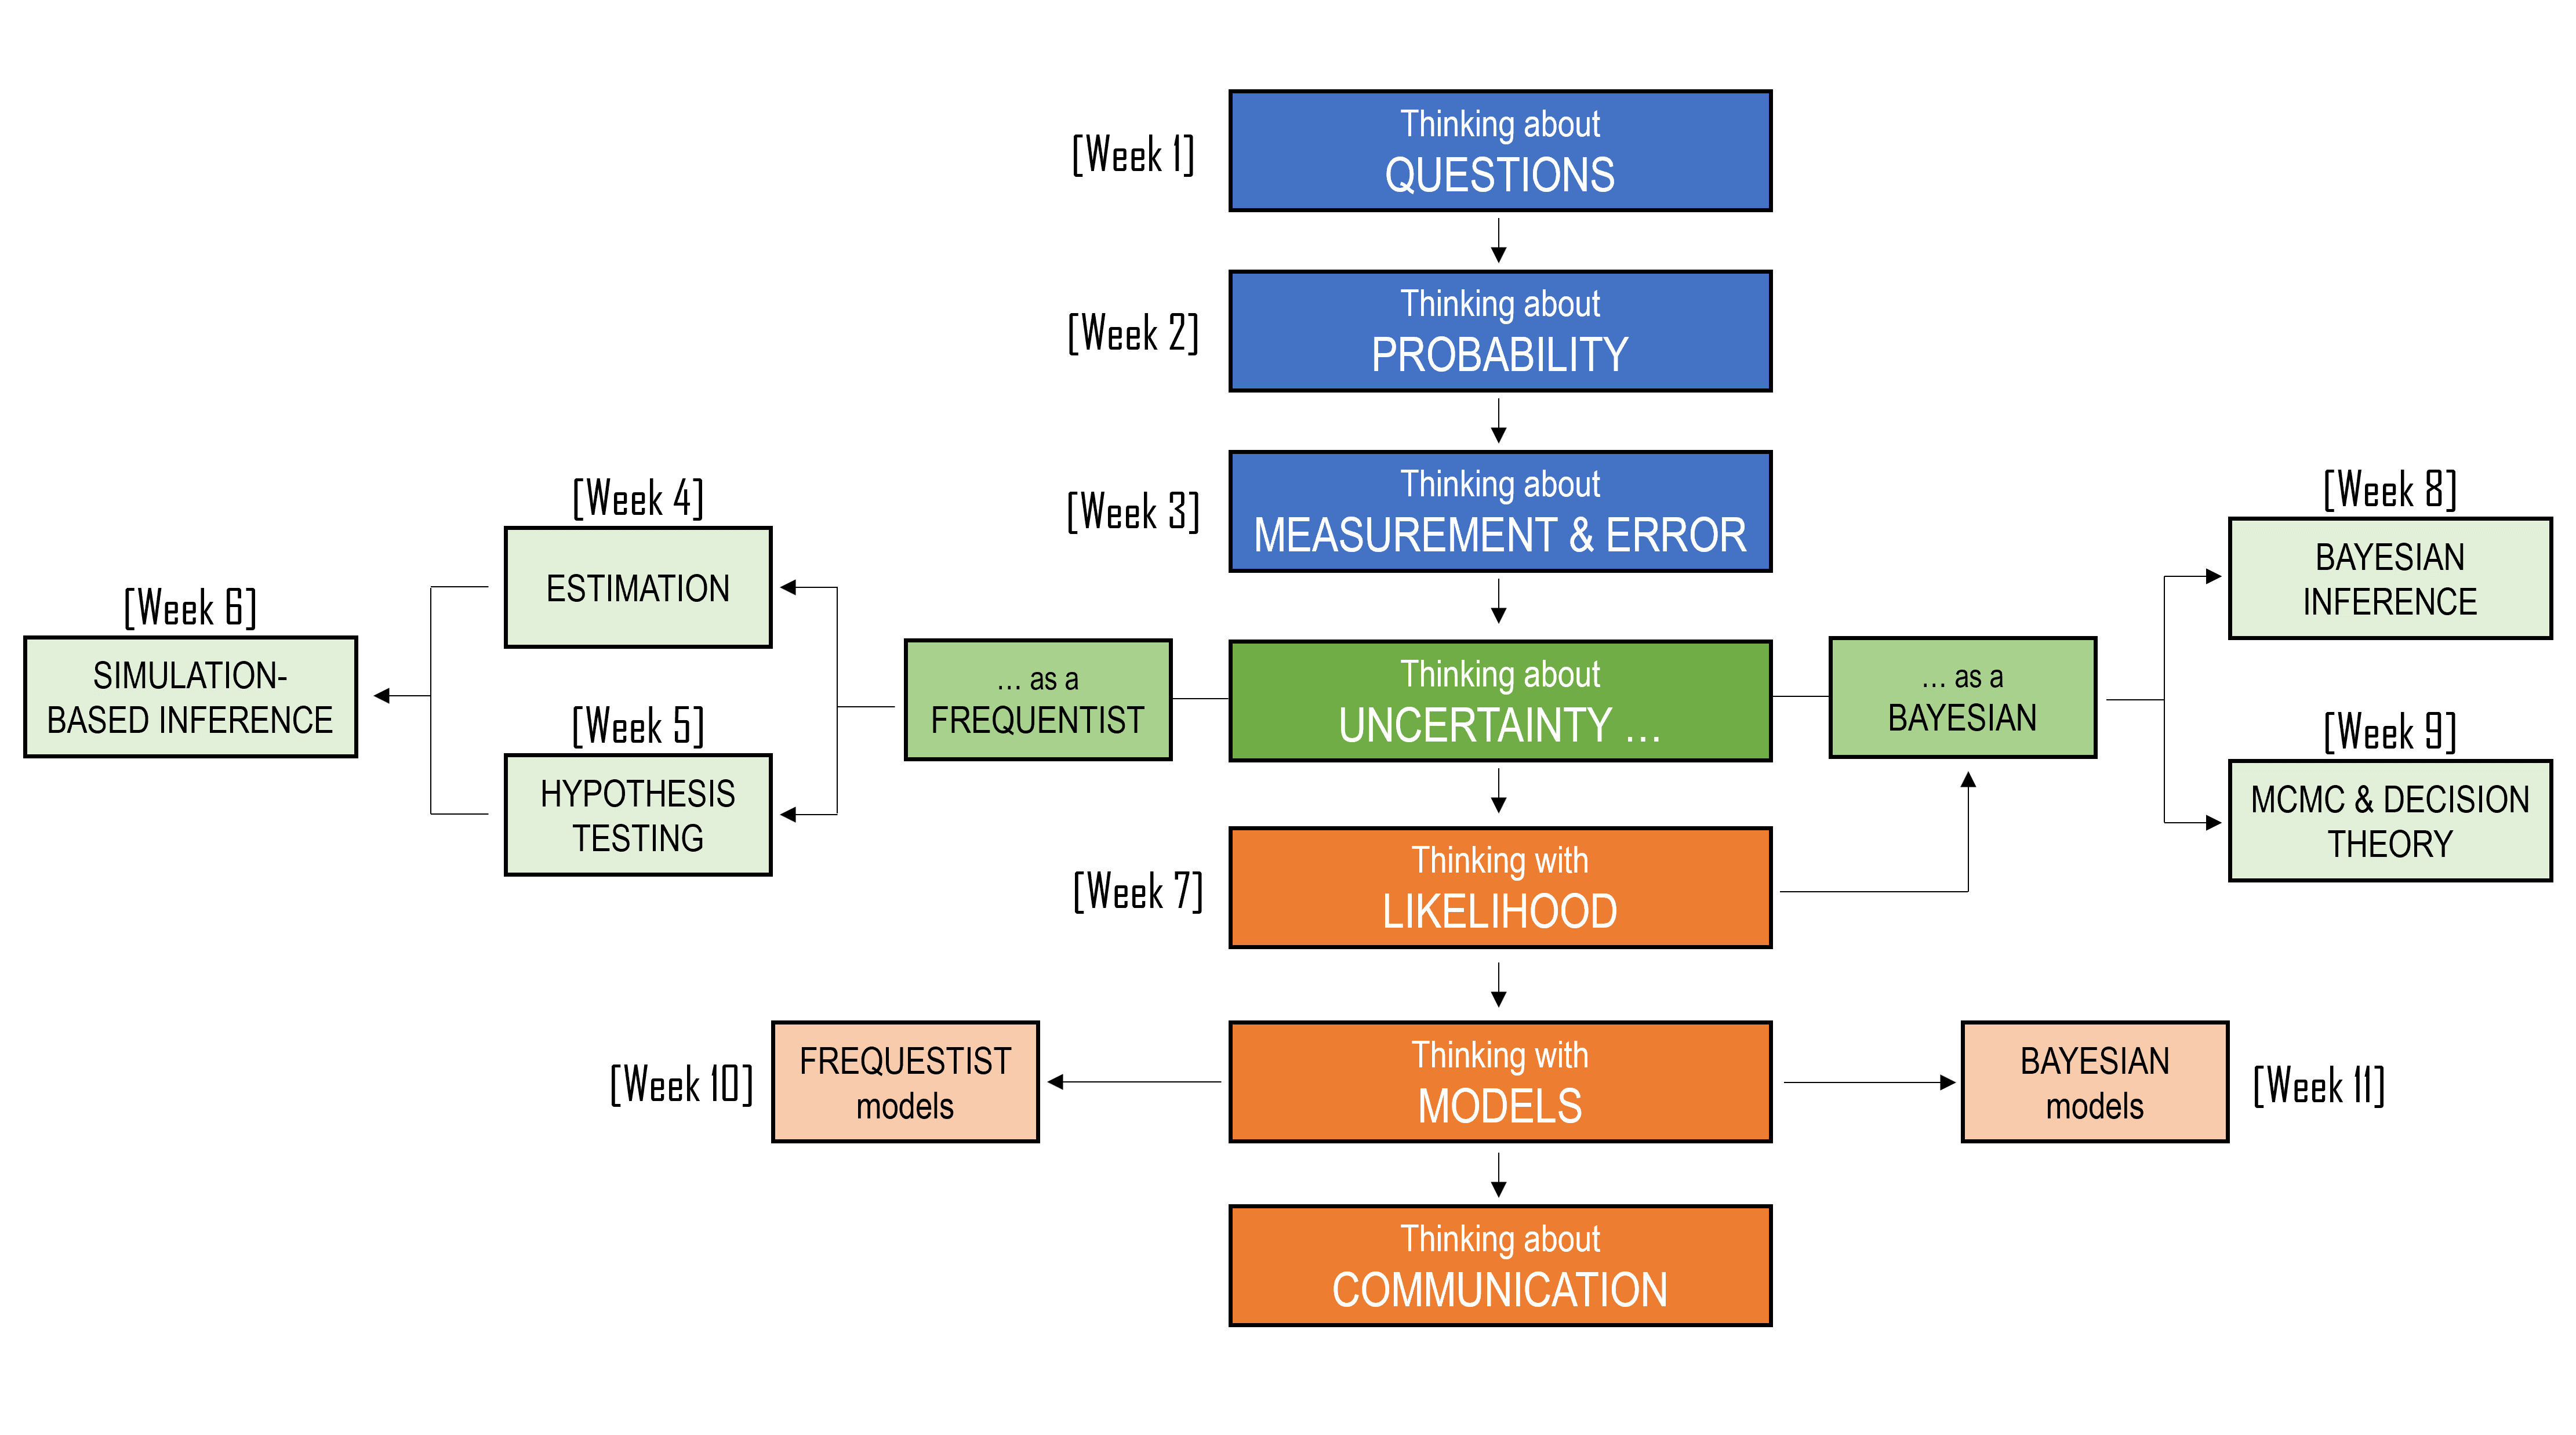
\includegraphics[width=14.81in,height=\textheight,keepaspectratio]{images/unit_outline7.png}

By the end of the unit, you should be more confident not only in doing
statistical analysis, but in explaining what it means. You should be
able to recognise uncertainty, communicate it clearly, and use
statistical models thoughtfully.

ETC2420/5242 has evolved over many years with input from hundreds of
students and teaching staff. Their curiosity, feedback, and creativity
have shaped the examples, visuals, and teaching strategies in these
pages. My hope is that this book helps you develop that habit of mind:
curious, careful, sceptical, and evidence-based.

\bookmarksetup{startatroot}

\chapter{Better Questions}\label{better-questions}

\begin{tcolorbox}[enhanced jigsaw, arc=.35mm, bottomrule=.15mm, bottomtitle=1mm, breakable, colback=white, colbacktitle=quarto-callout-note-color!10!white, colframe=quarto-callout-note-color-frame, coltitle=black, left=2mm, leftrule=.75mm, opacityback=0, opacitybacktitle=0.6, rightrule=.15mm, title=\textcolor{quarto-callout-note-color}{\faInfo}\hspace{0.5em}{Learning Objectives}, titlerule=0mm, toprule=.15mm, toptitle=1mm]

By the end of this chapter, you should be able to:

\begin{enumerate}
\def\labelenumi{\arabic{enumi}.}
\tightlist
\item
  Explain why statistical thinking begins with asking clear and useful
  questions.
\item
  Distinguish between reasoning before an outcome is known and reasoning
  after an outcome has occurred.
\item
  Describe the relationship between what could have happened and what
  did happen.
\item
  Explain why probability provides a language for uncertainty, rather
  than a guarantee of certainty.
\item
  Recognise how vague expressions of uncertainty, such as ``unlikely''
  or ``a fair chance'', can lead to misunderstanding.
\item
  Explain why rare events are not impossible, and why rare descriptions
  are not necessarily unique.
\item
  Use simple probability rules to reason about uncertain events,
  including addition, multiplication, overlap, and independence.
\item
  Explain why pieces of evidence should not be combined without
  considering whether they are independent.
\item
  Identify when a probability calculation answers the wrong question.
\item
  Reframe intuitive questions into better statistical questions
  involving uncertainty, evidence, comparison, assumptions, and process.
\end{enumerate}

\end{tcolorbox}

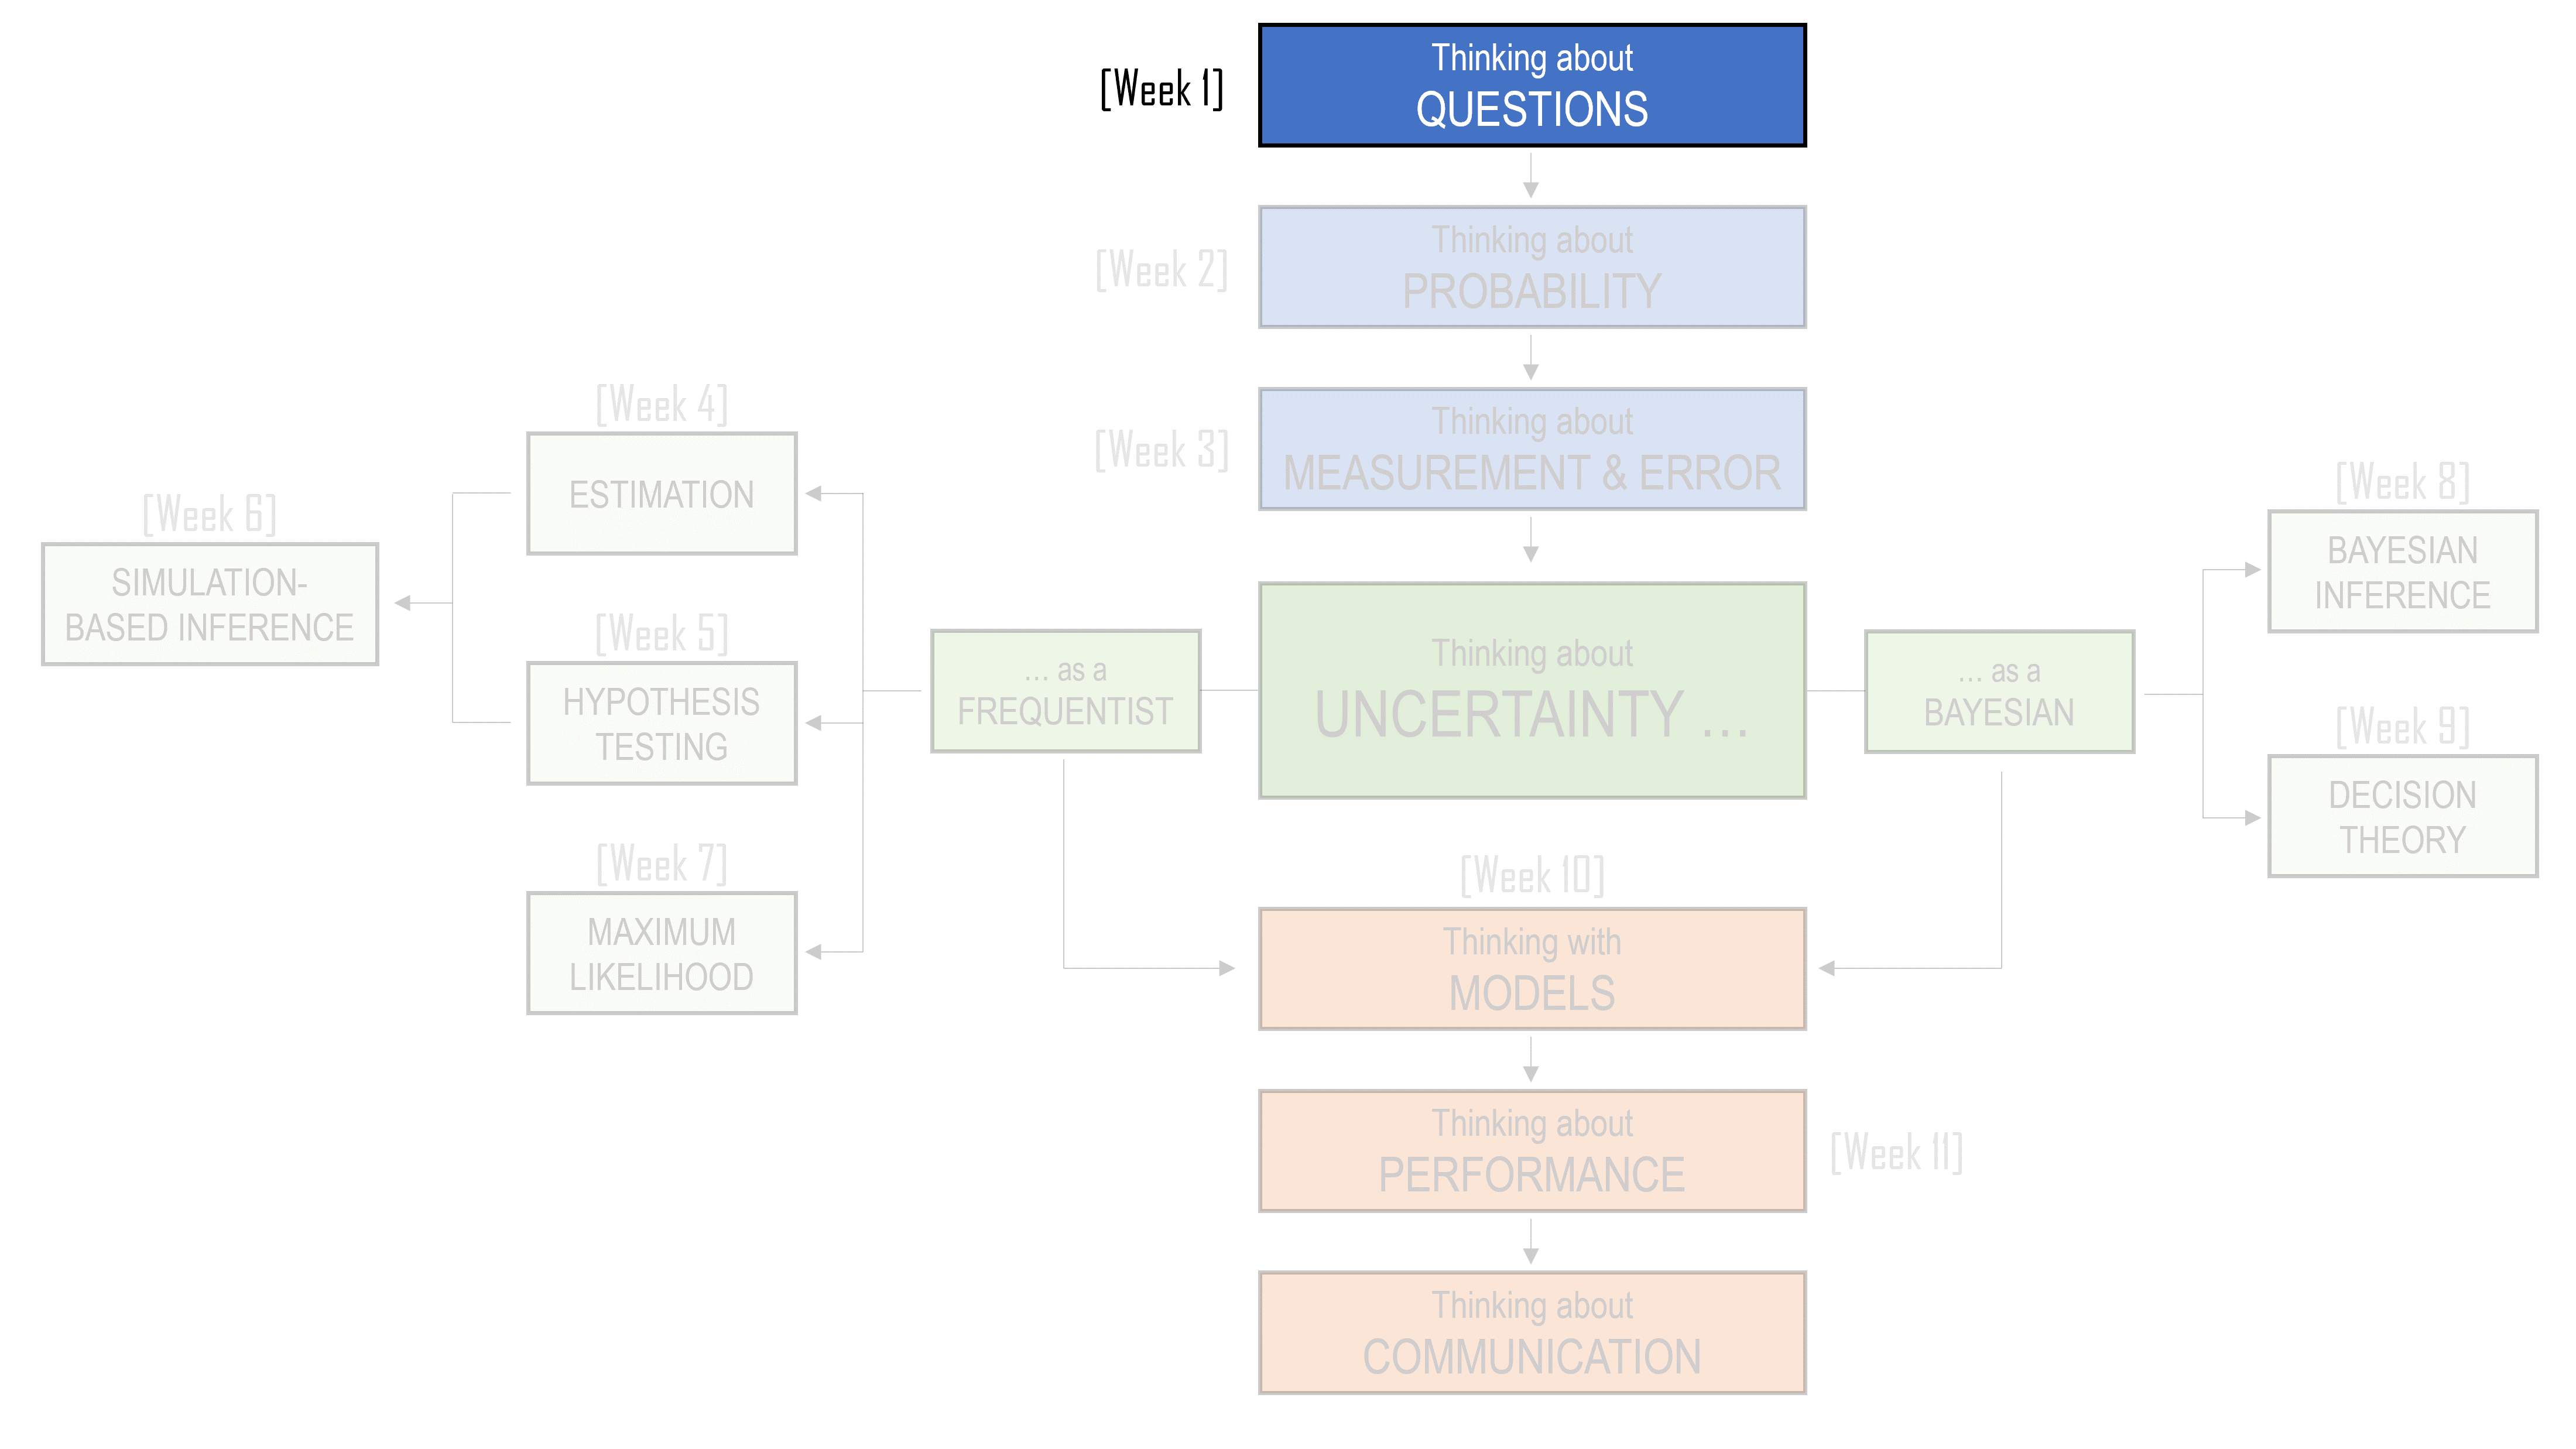
\includegraphics[width=14.67in,height=\textheight,keepaspectratio]{images/chapter1/outline.png}

\section{Three Boats, Many Possible
Futures}\label{three-boats-many-possible-futures}

After the Vietnam War (1975), millions of Vietnamese people left the
country, many as refugees. A large number fled by sea and became known
as the Vietnamese boat people. They travelled in crowded and often
fragile boats, hoping to reach refugee camps in places such as Hong
Kong, Malaysia, Indonesia, Thailand, or the Philippines. From there,
some were resettled in countries such as Australia, the United States,
Canada, and France.

The journeys were dangerous. Boats faced storms, hunger, dehydration,
mechanical failure, piracy, and the possibility of being turned away
before reaching land.

\begin{figure}[H]

{\centering 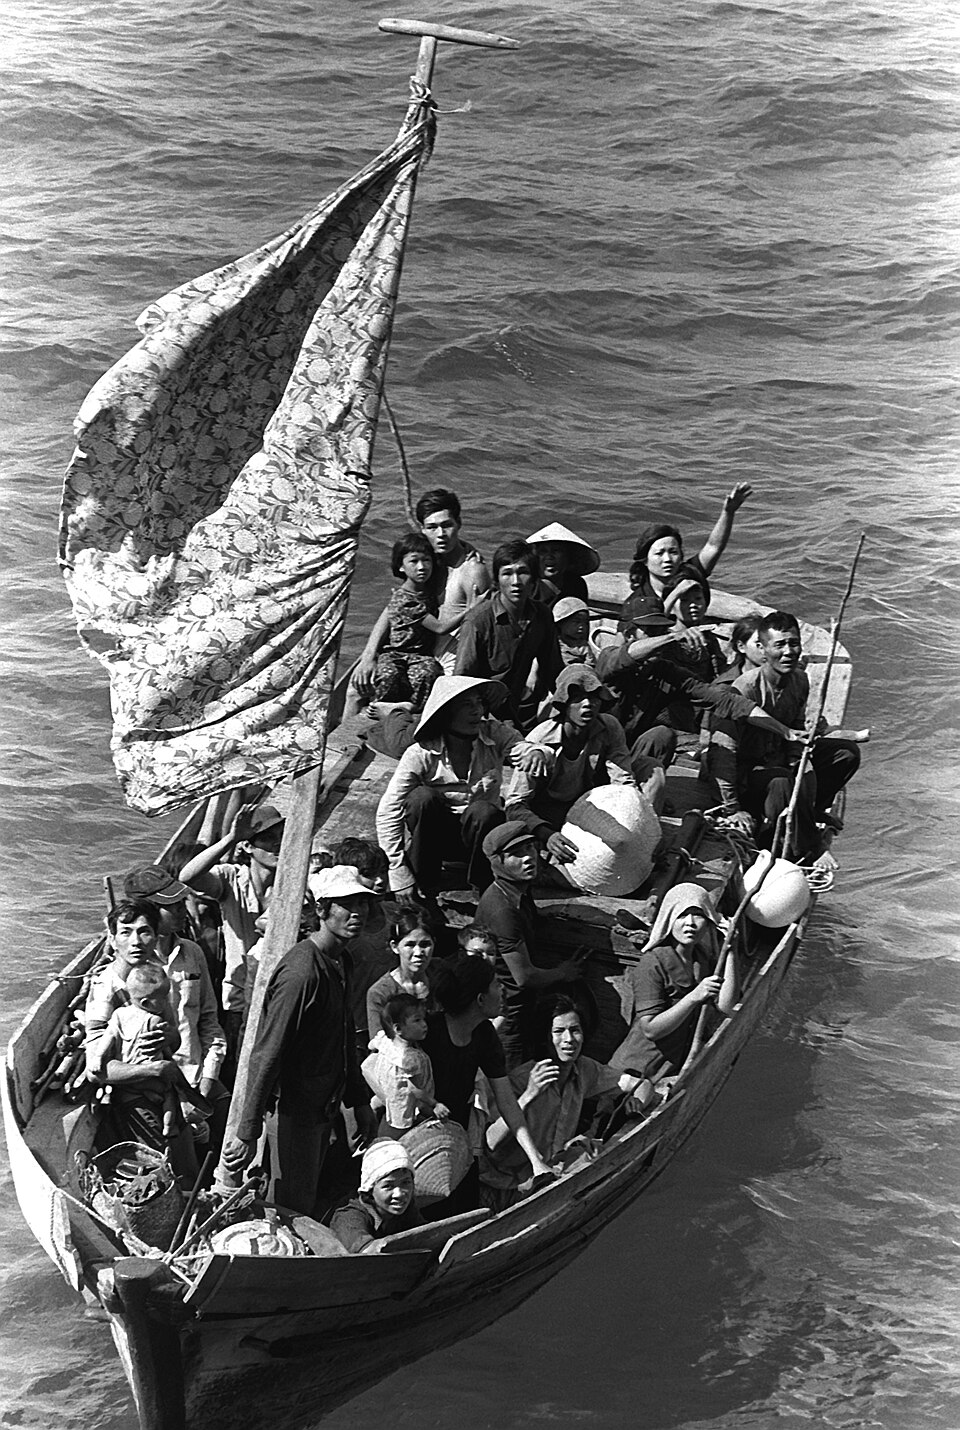
\includegraphics[width=3.2in,height=\textheight,keepaspectratio]{images/chapter1/boatpeople.JPEG}

}

\caption{Image Source: PH2 Phil Eggman}

\end{figure}%

This history is also part of my own family history, even though it
happened before I was born.

More than 70 members of my extended family attempted to flee Vietnam by
boat. They did not all travel together. Instead, the family split into
three groups, across three different boats, each heading toward a
different destination. This decision was not accidental. The reasoning
was painfully simple: if the whole family travelled on one boat, then
everyone would share the same fate. If that boat reached safety,
everyone survived. If that boat was lost, everyone was lost.

During a family dinner, one of my uncles was recalling the events of
that day and gave me a simple explanation for the decision to split
across three boats:

\begin{quote}
``This way, we have a higher chance of at least some family members
surviving.''
\end{quote}

That sentence is about probability, although nobody needed a formula to
understand it. It is about uncertainty, risk, and the terrible logic of
making decisions when every option is dangerous.

So how did this strategy work out for my family?

\begin{itemize}
\tightlist
\item
  Two boats made it safely to different refugee camps. From there, one
  side of the family was eventually sent to America, and the other to
  Australia.
\item
  To this day, we have no information about those on the third boat. No
  one knows what happened: whether they sank at sea, were attacked by
  pirates, or met some other fate that was never recorded and never
  returned to us as an answer.
\end{itemize}

My grandmother once told me that:

\begin{quote}
``The decision about who went on which boat had nothing to do with you.
After all, you did not exist yet. But if that decision had gone
differently, you would may have been born.''
\end{quote}

After the fact, the story sounds fixed: two boats made it, one did not.
But before the journey, nothing was fixed. All three boats might have
made it. None might have made it. The boat carrying the people who would
later become my parents might not have made it. Another branch of the
story might have led to a world in which I was never born.

This is a painful way to begin a statistics chapter. But it is also an
honest one. Statistics is not only about games of chance or classroom
examples. It is about how we think when outcomes are uncertain and the
stakes are real.

The decision to split across three boats shows one of the deepest ideas
in statistical thinking: uncertainty is not just something we calculate
after the fact. It shapes decisions before we know the outcome.
Splitting the family across three boats did not remove the danger. It
did not make the sea safer, the weather calmer, or the journey fairer.
But it changed the structure of the risk. It made survival less
dependent on a single outcome.

When we study probability, we often ask:

\begin{quote}
What could happen?
\end{quote}

When we study data, we often ask:

\begin{quote}
What did happen?
\end{quote}

Statistical thinking asks us to hold both questions together. We look at
what happened, but we also try to understand what else might have
happened, how likely different outcomes were, and what decisions made
sense under uncertainty. That is why this chapter begins not with a
formula, but with a question.

\begin{quote}
How do we think clearly when we do not know what will happen?
\end{quote}

\section{Before We Know the Outcome}\label{before-we-know-the-outcome}

Once we know what happened, it is tempting to tell the story as if it
could only have happened that way.

\begin{quote}
Two boats made it. One boat did not. One branch of the family was
eventually sent to America. Another branch was eventually sent to
Australia. The people on the third boat were never heard from again.
\end{quote}

Looking backwards, the outcome feels fixed. It becomes the story. This
happened, then that happened, and then this is where we ended up. But
that is not how uncertainty feels before the outcome is known.

Statistics often begins in the space between what could happen and what
did happen. Before the outcome, we face a set of possibilities. After
the outcome, we observe only one of them. The difficulty is that
decisions must usually be made before we know which possibility will
become real.

This is true in ordinary situations as well as extraordinary ones.

\begin{itemize}
\tightlist
\item
  Before a doctor recommends a treatment, they do not know exactly how a
  particular patient will respond.
\item
  Before a student sits an exam, they do not know exactly which
  questions will appear.
\item
  Before a business launches a product, it does not know how customers
  will react.
\item
  Before a government introduces a policy, it does not know exactly what
  effects the policy will have.
\item
  Before we collect data, we do not know exactly what pattern the data
  will show.
\end{itemize}

In each case, there is a difference between asking the question before
the outcome and asking it afterwards.

After an exam, a student might say:

\begin{quote}
I should have studied that topic more.
\end{quote}

But before the exam, the question was different:

\begin{quote}
Given limited time and uncertainty about what will be assessed, how
should I decide what to study?
\end{quote}

After a patient improves, it may be tempting to say:

\begin{quote}
The treatment worked.
\end{quote}

But before comparing that patient with what might have happened
otherwise, the better question is:

\begin{quote}
Did the patient improve because of the treatment, or would they have
improved anyway?
\end{quote}

After an investment rises in value, someone might say:

\begin{quote}
It was obviously a good investment.
\end{quote}

But before the outcome was known, the better question was:

\begin{quote}
Was this a good decision given the risks and information available at
the time?
\end{quote}

This distinction matters because good outcomes do not always come from
good decisions, and bad outcomes do not always come from bad decisions.
Sometimes a risky decision works out. Sometimes a careful decision ends
badly. Judging a decision only by its outcome can be misleading, because
it ignores the uncertainty that existed at the time the decision was
made.

Statistical thinking asks us to resist that temptation. It asks us to
imagine the range of outcomes that could have occurred, not only the one
that did occur. It asks us to think about how likely different outcomes
were, what evidence was available at the time, and whether the decision
made sense before the result was known.

This is why probability matters. Probability gives us a language for
talking about possible outcomes before we know which one will happen.
But statistics is not only about probability. It is also about data.
Once something has happened, data give us traces of the outcome. We can
count, measure, compare, and model what we observe. But data always
arrive after some process has already taken place. They show us what
happened, not everything that could have happened.

Likewise, a dataset is not the whole story. It is one realised version
of a larger set of possibilities.

This unit is about learning how to think in that space. It is about
using probability to reason about what could happen, using data to
understand what did happen, and using statistical methods to connect the
two. Along the way, we will learn technical tools: sample spaces,
simulations, confidence intervals, hypothesis tests, regression models,
and other methods. But the tools are not the main point. The main point
is learning how to ask clearer questions when the world is uncertain.

That means asking questions such as:

\begin{quote}
What are the possible outcomes?
\end{quote}

\begin{quote}
What evidence do we have?
\end{quote}

\begin{quote}
What are we comparing?
\end{quote}

\begin{quote}
How much variation is there?
\end{quote}

\begin{quote}
Could this pattern have occurred by chance?
\end{quote}

\begin{quote}
What assumptions are we making?
\end{quote}

\begin{quote}
What would have happened otherwise?
\end{quote}

These questions are the foundation of the unit. The formulas and methods
we learn later are ways of answering them more carefully.

That is why, throughout this unit, we will keep returning to two
questions:

\begin{quote}
What could have happened?
\end{quote}

and

\begin{quote}
What did happen?
\end{quote}

The first question asks us to think about possibility, uncertainty, and
chance. The second asks us to look carefully at evidence. Statistical
thinking begins when we learn to hold these questions together.

If we focus only on what could have happened, we may become lost in
speculation. If we focus only on what did happen, we may treat the
observed outcome as inevitable. Statistics lives between these extremes.
It uses data from the world that did happen to reason about uncertainty,
variation, and the worlds that might have happened instead.

This is one reason the first question we ask is rarely the final
question we need.

We may begin with:

\begin{quote}
What happened?
\end{quote}

But often we need to ask:

\begin{quote}
What else could have happened?
\end{quote}

We may begin with:

\begin{quote}
Did this decision work out?
\end{quote}

But often we need to ask:

\begin{quote}
Was this a good decision given what was known at the time?
\end{quote}

We may begin with:

\begin{quote}
Is this result surprising?
\end{quote}

But often we need to ask:

\begin{quote}
Surprising compared with what possibilities?
\end{quote}

We may begin with:

\begin{quote}
Can we see a pattern?
\end{quote}

But often we need to ask:

\begin{quote}
Could this pattern have appeared just by chance?
\end{quote}

The goal of statistics is not to remove uncertainty from life. It cannot
do that. The goal is to help us think more clearly when uncertainty is
present.

And that begins by learning to ask better questions.

\section{A First Language for
Uncertainty}\label{a-first-language-for-uncertainty}

Learning to ask better questions requires a language for uncertainty. In
everyday life, we often speak about uncertainty vaguely. We say that
something is \emph{unlikely}, \emph{possible}, \emph{risky}, \emph{a
good chance}, \emph{a long shot}, or \emph{almost certain}. These words
are useful, but they can also be slippery. One person's \emph{unlikely}
might be another person's \emph{still worth worrying about.} One
person's \emph{good chance} might mean 60 percent, while another person
might use the same phrase for 90 percent.

\begin{tcolorbox}[enhanced jigsaw, arc=.35mm, bottomrule=.15mm, bottomtitle=1mm, breakable, colback=white, colbacktitle=quarto-callout-note-color!10!white, colframe=quarto-callout-note-color-frame, coltitle=black, left=2mm, leftrule=.75mm, opacityback=0, opacitybacktitle=0.6, rightrule=.15mm, title=\textcolor{quarto-callout-note-color}{\faInfo}\hspace{0.5em}{A cautionary tale about expressing uncertainty}, titlerule=0mm, toprule=.15mm, toptitle=1mm]

After Fidel Castro's forces came to power in Cuba in 1959, the CIA
worked with Cuban exiles on a plan to remove the new government and
replace it with one more favorable to the United States. When John F.
Kennedy became president in January 1961, the invasion plan was already
far advanced.

\begin{figure}[H]

{\centering 
\includegraphics[width=3.25in,height=\textheight,keepaspectratio]{images/chapter1/bayofpigs.png}

}

\caption{Image Source: https://www.bbc.com/news/}

\end{figure}%

However, the US Joint Chiefs of Staff were doubtful about its prospects
and estimated its chance of success at only about 30\%. In a report
prepared for Kennedy, Brigadier General David Gray expressed this as

\begin{quote}
``a fair chance.''
\end{quote}

Kennedy, however, appears to have understood the phrase more
optimistically, as suggesting that the operation had a reasonable
likelihood of success. He later approved the invasion. On 17 April 1961,
around 1,500 Cuban exiles landed at the Bay of Pigs on Cuba's southern
coast, where they encountered fierce resistance led by Castro. More than
one hundred were killed and most of the remaining fighters were
captured. The failed invasion was a major humiliation for the United
States and helped push Cuba closer to the Soviet Union, contributing to
the tensions that culminated in the Cuban Missile Crisis the following
year.

Years later, General Taylor carried out an enquiry of this disaster and
reported

\begin{quote}
``There is a time when you can't advise by innuendos and suggestions.
You have to look him in the eye and say, ``I think it's a lousy idea, Mr
President. The chances of us succeeding are about one in ten.''\,'
\end{quote}

\end{tcolorbox}

Probability gives us a more careful language. It does not remove
uncertainty, and it does not guarantee that we will make the right
decision. What it does is help us organise our thinking. It asks us to
be clearer about what could happen, how likely different outcomes are,
and what assumptions we are making when we reason about an uncertain
situation.

\begin{tcolorbox}[enhanced jigsaw, arc=.35mm, bottomrule=.15mm, bottomtitle=1mm, breakable, colback=white, colbacktitle=quarto-callout-important-color!10!white, colframe=quarto-callout-important-color-frame, coltitle=black, left=2mm, leftrule=.75mm, opacityback=0, opacitybacktitle=0.6, rightrule=.15mm, title=\textcolor{quarto-callout-important-color}{\faExclamation}\hspace{0.5em}{Note about probability}, titlerule=0mm, toprule=.15mm, toptitle=1mm]

Note: we will cover more concepts about probability in Chapter 2
(Thinking about Probability), but it will be good to briefly introduce
it here.

\end{tcolorbox}

\section{The Ancient Greeks: Masters of certainty, not
uncertainty}\label{the-ancient-greeks-masters-of-certainty-not-uncertainty}

It may seem strange that probability developed so late in human history.
People have always faced uncertainty. They have always gambled, made
risky decisions, interpreted signs, and wondered what the future might
bring. So why did it take so long for probability to become a formal
part of mathematics? One useful place to begin is ancient Greece.

The ancient Greeks made extraordinary contributions to mathematics. Much
of the style of mathematics we still learn today comes from them:
definitions, axioms, logical arguments, proofs, theorems, and then more
proofs. Greek mathematics aimed at certainty. A theorem in geometry was
not a guess, a pattern, or a rough guide. It was something to be
demonstrated through reason.

\begin{figure}[H]

{\centering 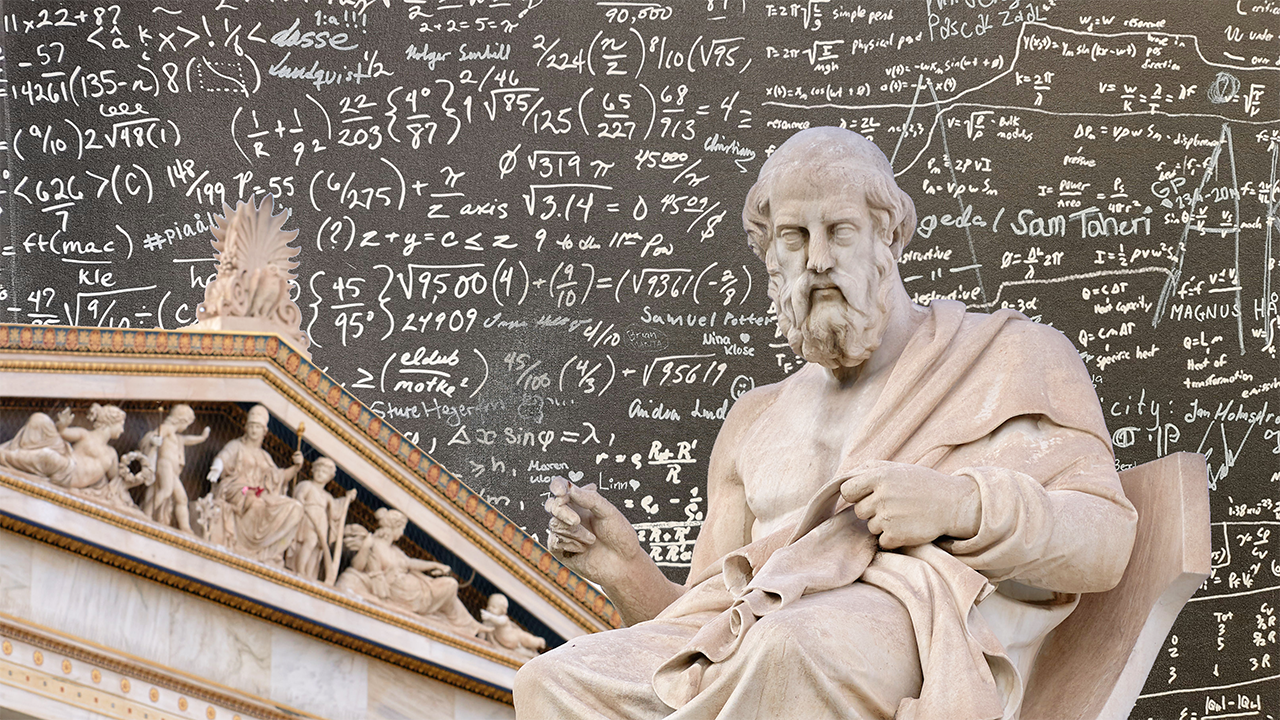
\includegraphics[width=4.27in,height=\textheight,keepaspectratio]{images/chapter1/ancientgreeks.png}

}

\caption{Image Source: Letters and Science}

\end{figure}%

Euclid's geometry is the classic example. Starting from a small number
of assumptions, Greek mathematicians proved results about lines, angles,
triangles, circles, and other shapes. Their work was so powerful that it
helped people reason about the shape of the Earth and even estimate its
size. This was mathematics as certainty: begin with agreed foundations,
follow the logic carefully, and arrive at a conclusion that must be
true.

But probability asks for a different kind of thinking.

Probability is not usually about what must happen. It is about what
might happen. It is about situations where several outcomes are possible
and we do not know in advance which one will occur. That makes
probability feel different from geometry. A geometric proof promises
certainty. A probability statement accepts uncertainty and tries to
reason within it.

That distinction helps explain why the Greeks, despite their
mathematical brilliance, did not develop a theory of probability. They
had games of chance, but they did not turn those games into a formal
mathematics of chance.

Instead of modern dice, the Greeks used objects called astragali. These
were made from the heel bones of animals. They could be tossed in games,
somewhat like dice, although they were not symmetrical in the way modern
dice are. Different sides were not equally likely to land face up. Some
outcomes were more common than others.

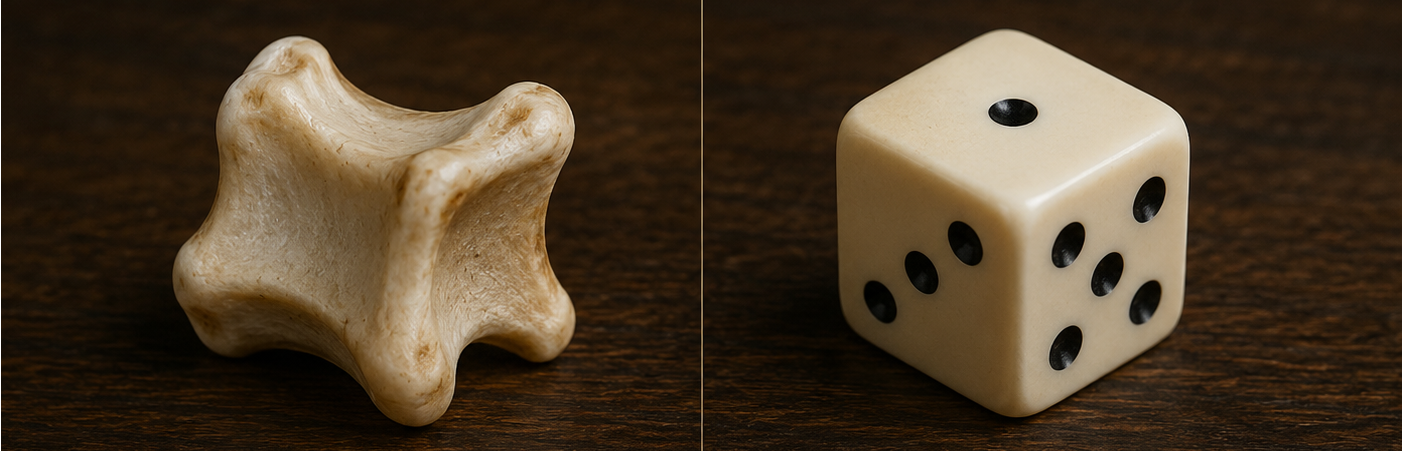
\includegraphics[width=4.67in,height=\textheight,keepaspectratio]{images/chapter1/astragli.png}

This is already a probability problem. A modern statistician might ask:

\begin{quote}
What are the possible outcomes of an astragalus toss?
\end{quote}

and:

\begin{quote}
Are those outcomes equally likely?
\end{quote}

and:

\begin{quote}
If we toss several astragali, how often should different combinations
occur?
\end{quote}

But that is not how the Greeks generally approached the problem. They
used astragali in games and in religious practices, including attempts
to seek guidance from oracles. The toss was not necessarily seen as the
result of a random process with regularities that could be studied. It
might instead be interpreted as a sign, a message, or the will of the
gods. If an outcome is understood as divine will, then probability is
not the natural question to ask. The question is not:

\begin{quote}
How often would this outcome occur in repeated tosses?
\end{quote}

The question becomes:

\begin{quote}
What does this outcome mean?
\end{quote}

This is a very different way of thinking.

There was also a philosophical obstacle. Greek mathematics valued
certainty. Probability, by contrast, deals in uncertainty, likelihood,
and partial knowledge. To a mind trained to value proof, a probabilistic
argument may look weak or suspicious. It does not say, ``This must be
true.'' It says something more modest: ``Given what we know, this is
more likely than that.''

But in real life, that modest kind of reasoning is often exactly what we
need.

When we ask

\begin{itemize}
\tightlist
\item
  whether it will rain,
\item
  whether a treatment will help,
\item
  whether a witness is reliable,
\item
  whether a pattern in data is surprising, or
\item
  whether a decision is worth the risk,
\end{itemize}

we are usually not in the world of geometric certainty. We are in the
world of uncertain evidence and possible outcomes. This is the world
probability was built for.

So the lesson from the Greeks is not that they were bad mathematicians.
The opposite is true. They were so successful at one kind of mathematics
that another kind of reasoning remained underdeveloped. Geometry gave
them a language for certainty. Probability would later become a language
for uncertainty.

In statistics, we rarely get the kind of certainty found in a geometric
proof. We work with data that are incomplete, measurements that are
imperfect, samples that vary, and conclusions that carry uncertainty.
Our task is not to pretend that uncertainty has disappeared. Our task is
to reason carefully while uncertainty remains. This is why probability
is more than a calculation. It is a different intellectual habit. It
teaches us to ask questions such as:

\begin{quote}
What outcomes are possible?
\end{quote}

\begin{quote}
Are they equally likely?
\end{quote}

\begin{quote}
What assumptions are we making?
\end{quote}

\begin{quote}
What would we expect to happen over many repetitions?
\end{quote}

\begin{quote}
How should we change our judgement when we receive new evidence?
\end{quote}

These are not questions of pure certainty. They are questions for a
world in which the future is not yet known, the evidence is incomplete,
and several outcomes remain possible.

\section{The Ancient Romans and The Problem of
Half-Truths}\label{the-ancient-romans-and-the-problem-of-half-truths}

The Ancient Greeks were drawn to mathematics as a search for certainty.
They gave us geometry, proof, axioms, and the ideal of conclusions that
follow necessarily from first principles.

The Romans were different. They were less interested in mathematics as
abstract beauty and more interested in mathematics as a practical tool.
They wanted measurement, counting, engineering, administration, military
planning, and law. That practical orientation matters for the history of
probability.

Probability does not usually begin with certainty. It begins when
certainty is unavailable. It begins when we have partial information,
conflicting testimony, incomplete evidence, and decisions that must be
made anyway. In that sense, the Roman world was closer to the world of
statistics than the Greek world of geometry. The Romans were not asking
only:

\begin{quote}
What can be proved with certainty?
\end{quote}

They were also asking:

\begin{quote}
What should we believe when the evidence is incomplete?
\end{quote}

That is a statistical question.

One of the most important Roman figures in this story is Marcus Tullius
Cicero. Cicero was a statesman, lawyer, philosopher, and writer who
lived in the first century BCE. He was not a mathematician in the Greek
sense, but he understood something deeply important about uncertainty:
life often requires judgement before proof is complete.

\begin{figure}[H]

{\centering 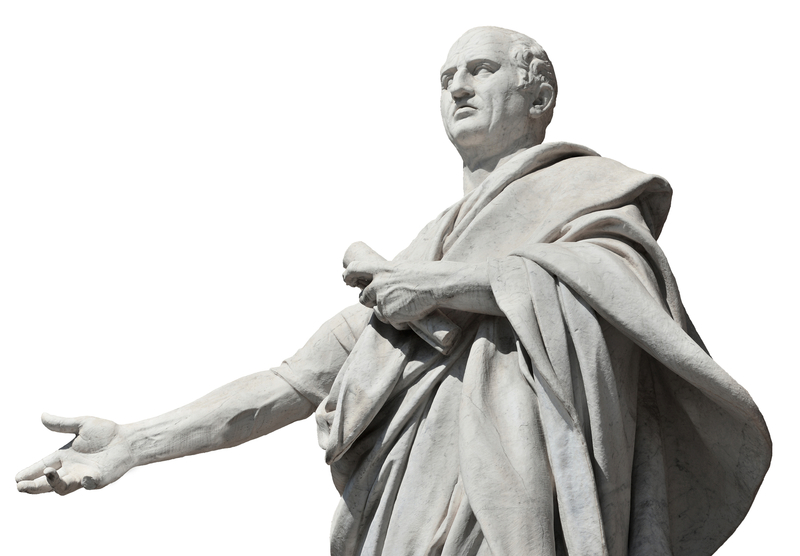
\includegraphics[width=2.67in,height=\textheight,keepaspectratio]{images/chapter1/cicero.jpg}

}

\caption{Marcus Tullius Cicero}

\end{figure}%

Cicero argued against the idea that unusual gambling outcomes should
automatically be interpreted as divine intervention. If someone plays a
game often enough, rare events will sometimes occur. A surprising throw
does not necessarily mean that the gods have intervened. It may simply
be the kind of thing that happens when chance is allowed to operate
repeatedly. This is a simple idea, but it is a powerful one.

Even today, people often treat rare events as if they must have special
explanations. Someone wins the lottery and says the number came to them
in a dream. A team wins several games in a row and commentators talk
about momentum. A student performs unusually well on one assessment and
we may be tempted to say they have suddenly ``figured it out.''
Sometimes there is a real explanation. But sometimes randomness produces
streaks, clusters, surprises, and coincidences.

Cicero's insight was that chance does not mean chaos. An event can be
unpredictable in a particular instance and still be understandable as
part of a broader pattern.

For example, suppose a fair die is rolled. The probability of rolling a
six is:

\[P(\text{six}) = \frac{1}{6}\]

Rolling a six is uncertain. Before the die is rolled, we do not know
whether it will happen. But if the die is rolled many times, it would
not be surprising to see sixes appear again and again. A six is not
mysterious simply because it was uncertain beforehand.

Even two sixes in a row do not require a supernatural explanation. If
the rolls are independent, then:

\[P(\text{six and then six}) = \frac{1}{6} \times \frac{1}{6} = \frac{1}{36}\]

A probability of (1/36) is small, but it is not impossible. If many
people roll dice many times, outcomes with probability (1/36) will occur
regularly somewhere. Probability helps us see that a rare event is not
the same as an impossible event, and that a surprising outcome is not
automatically evidence of a hidden cause.

The Roman contribution becomes even more interesting when we turn to
law.

\begin{itemize}
\tightlist
\item
  Legal decision-making is full of uncertainty.
\item
  Witnesses may disagree.
\item
  Evidence may be incomplete.
\item
  A person may seem suspicious but not certainly guilty.
\item
  A document may be partly reliable.
\item
  A testimony may be plausible but not decisive.
\item
  Courts must often make decisions in the space between ignorance and
  certainty.
\end{itemize}

In this setting, the Romans developed the idea of partial proof. A piece
of evidence might not establish a claim completely, but it might still
count for something. It might be, in effect, a \emph{half proof}.

At first, this seems like a sensible idea. Not all evidence has the same
strength.

\begin{itemize}
\tightlist
\item
  One witness might be uncertain. Two witnesses might be more
  convincing.
\item
  A confession might be stronger than a rumour.
\item
  Physical evidence might be stronger than hearsay.
\end{itemize}

Even today, we often speak this way. We say that evidence is weak,
strong, suggestive, compelling, or inconclusive. The Romans were trying
to do something recognisably statistical: they were trying to reason
with degrees of uncertainty.

The problem was how to combine those degrees. In some versions of Roman
legal reasoning, two half proofs could be treated as one complete proof.
Symbolically, this sounds like:

\[\frac{1}{2} + \frac{1}{2} = 1\]

As arithmetic, that is true. But as a way of combining uncertain
evidence, it is not generally correct.

The mistake is subtle. A half proof is not the same kind of object as
half a loaf of bread. If I have half a loaf and you give me another
half, I have a whole loaf. But if I have one uncertain piece of evidence
and then receive another uncertain piece of evidence, I do not
necessarily have certainty. I may have stronger evidence, but not
perfect proof.

To see why, suppose each piece of evidence has a 50 percent chance of
being correct. That is, each has a 50 percent chance of being wrong. If
the two pieces of evidence are independent, then the probability that
both are wrong is:

\[P(\text{both wrong}) = \frac{1}{2} \times \frac{1}{2} = \frac{1}{4}\]

So the probability that at least one of them is right is:

\[P(\text{at least one right}) = 1 - P(\text{both wrong})\]

\[= 1 - \frac{1}{4}\]

\[= \frac{3}{4}\]

Two independent half proofs therefore do not produce certainty. They
produce something closer to three-quarters proof, under these
assumptions. This is an important distinction.

The Roman rule treated partial evidence as if it could simply be added
until certainty was reached. Probability teaches us that uncertain
evidence does not usually work that way. If each piece of evidence can
be wrong, then even several pieces of evidence may leave some
possibility of error.

For example, suppose three independent pieces of evidence each have a 50
percent chance of being wrong. The probability that all three are wrong
is:

\[\left(\frac{1}{2}\right)^3 = \frac{1}{8}\]

So the probability that at least one is right is:

\[1 - \frac{1}{8} = \frac{7}{8}\]

That is stronger than \(\frac{3}{4}\), but still not certainty.

With four such pieces of evidence:

\[1 - \left(\frac{1}{2}\right)^4 = 1 - \frac{1}{16} = \frac{15}{16}\]

Again, the evidence becomes stronger, but it does not become perfect. No
finite number of uncertain pieces of evidence becomes absolute certainty
in this simple model. Each additional piece can reduce uncertainty, but
it does not remove it entirely.

This gives us one of the key lessons of probability:

\begin{quote}
Evidence can accumulate without becoming certainty.
\end{quote}

In statistics, we often work with conclusions that are well supported
but not guaranteed. A confidence interval may be narrow, but it does not
make error impossible. A hypothesis test may produce a small p-value,
but it does not prove a claim with certainty. A model may fit the data
well, but it is still a model. A sample may strongly suggest something
about a population, but the sample is not the population.

The Roman idea of half proofs is therefore useful not because it was
mathematically correct, but because it shows why probability is needed.
Once we admit that evidence can be partial, we need rules for reasoning
with partial evidence.

We need to ask:

\begin{quote}
How strong is each piece of evidence?
\end{quote}

\begin{quote}
Are the pieces of evidence independent?
\end{quote}

\begin{quote}
Are they pointing to the same conclusion?
\end{quote}

\begin{quote}
Could they share the same source of error?
\end{quote}

\begin{quote}
Does one piece of evidence change how we should interpret another?
\end{quote}

These questions matter because evidence is not always independent.

Suppose two witnesses give the same description of a person leaving the
scene of an accident. If the witnesses saw the event from different
positions, did not speak to each other, and had no shared source of
information, then their agreement may be quite informative. But if one
witness heard the description from the other, then the second testimony
is not independent evidence. It may sound like two pieces of evidence,
but it is closer to one piece repeated twice.

The same issue appears in data analysis. Suppose two variables in a
dataset seem to support the same conclusion. Before we treat them as
separate evidence, we need to ask whether they are genuinely separate.
Are they measuring different things, or are they two versions of the
same thing? For example, a person's income and the value of their house
may both tell us something about socioeconomic status, but they are not
independent pieces of information. Knowing one changes what we expect
about the other.

This is why independence is an important idea in probability.

If two events (A) and (B) are independent, then knowing that one
occurred does not change the probability of the other. In that case, we
can multiply probabilities:

\[P(A \text{ and } B) = P(A)P(B)\]

But if the events are not independent, this formula does not apply in
that simple form. We must think more carefully.

The Roman half-proof idea therefore leads us directly to another
important habit in statistical thinking:

\begin{quote}
Before combining evidence, ask whether the evidence is genuinely
separate.
\end{quote}

This habit will appear throughout the unit. It appears when we study
probability. It appears when we analyse survey data. It appears when we
compare groups. It appears when we think about experiments. It appears
when we build regression models. In each case, we need to understand not
only what evidence we have, but how that evidence was produced and how
the pieces of evidence relate to one another.

The Romans saw something important: uncertainty comes in degrees. A
claim does not have to be either completely proved or completely
unsupported. Evidence can be partial. Some claims are more plausible
than others. Some testimony is stronger than other testimony. Some
conclusions are better supported than others.

But the Romans also show us the danger of having the right intuition
without the right rules. They recognised half-truths, but they did not
yet have the mathematics to combine them properly.

\begin{tcolorbox}[enhanced jigsaw, arc=.35mm, bottomrule=.15mm, bottomtitle=1mm, breakable, colback=white, colbacktitle=quarto-callout-note-color!10!white, colframe=quarto-callout-note-color-frame, coltitle=black, left=2mm, leftrule=.75mm, opacityback=0, opacitybacktitle=0.6, rightrule=.15mm, title=\textcolor{quarto-callout-note-color}{\faInfo}\hspace{0.5em}{Roman Evidence}, titlerule=0mm, toprule=.15mm, toptitle=1mm]

As an example, the ancient Romans had established the following rule for
evidence against members of the church:

``\emph{A bishop should not be condemned except with seventy-two
witnesses. A cardinal priest should not be condemned except with
forty-four witnesses A cardinal deacon of the city of Rome without
thirty-six witnesses A subdeacon, acolyte, exorcist, lector, or
doorkeeper except with seven witnesses.}''

\begin{figure}[H]

{\centering 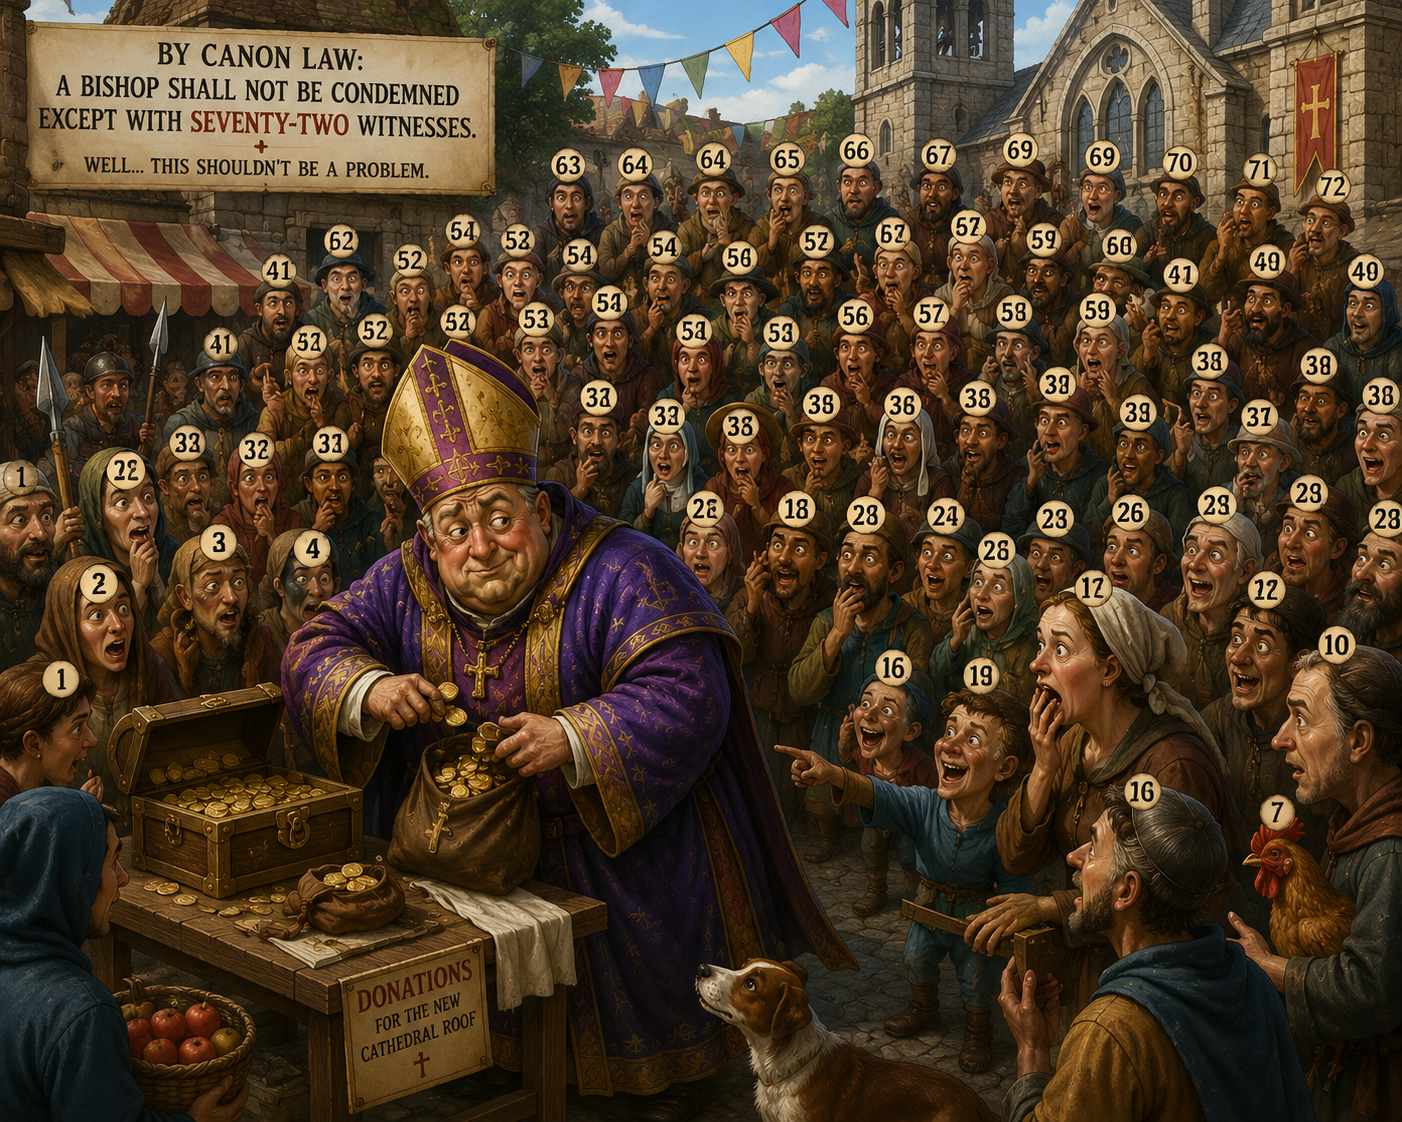
\includegraphics[width=4.67in,height=\textheight,keepaspectratio]{images/chapter1/bishop.png}

}

\caption{What happens to the bishop is there are only 71 witnesses?}

\end{figure}%

\end{tcolorbox}

This is why probability matters. It gives structure to uncertainty. It
helps us avoid treating partial evidence as certainty. It helps us see
when evidence should be added, when probabilities should be multiplied,
and when a calculation depends on an assumption such as independence.

\begin{tcolorbox}[enhanced jigsaw, arc=.35mm, bottomrule=.15mm, bottomtitle=1mm, breakable, colback=white, colbacktitle=quarto-callout-note-color!10!white, colframe=quarto-callout-note-color-frame, coltitle=black, left=2mm, leftrule=.75mm, opacityback=0, opacitybacktitle=0.6, rightrule=.15mm, title=\textcolor{quarto-callout-note-color}{\faInfo}\hspace{0.5em}{Case Study: Timothy Durham}, titlerule=0mm, toprule=.15mm, toptitle=1mm]

DNA evidence can sound almost impossibly strong. Imagine a jury hears
the following statement:

\begin{quote}
The DNA profile from the crime scene matches the suspect.
\end{quote}

At first, this can sound decisive. DNA feels scientific, precise, and
difficult to argue against. But the case of Timothy Durham shows why
statistical thinking asks us to slow down. In 1993, Timothy Durham was
convicted in Oklahoma for the rape of an 11-year-old girl. The evidence
against him included eyewitness identification, hair comparison
evidence, and DNA evidence. A laboratory analyst testified that a
genetic marker found in the crime-scene sample matched one of Durham's
markers. This did not uniquely identify him, but it was used to include
him in the suspect pool.

The DNA evidence sounded powerful because DNA evidence is often
presented using extremely small probabilities. A jury might hear
something like:

\begin{quote}
The probability that a randomly chosen person would match this DNA
profile is less than 1 in 1 billion
\end{quote}

A number like this can feel overwhelming. If the chance of a random
match is only:

\[\frac{1}{1,000,000,000}\]

then it is tempting to think that the suspect must be guilty.

In Durham's case, however, there was also evidence pointing in the other
direction. Eleven defence witnesses testified that he was in Dallas,
Texas, at a skeet shooting competition when the crime occurred. Records
were presented showing purchases he had made there, and a handwriting
expert confirmed that the signatures were his. Despite this evidence,
the jury believed the DNA evidence (or the number of 1 in one billion)
was stonger. They convicted him. He was sentenced to prison terms
totaling more than 3,000 years.

But there was another statistic that was not presented in this case: the
probability of laboratory error. A DNA result can also be wrong because
of the testing process itself. Samples can be mixed up, contaminated,
incompletely separated, mislabelled, misread, or incorrectly reported.
These errors may be rare, but they may be much more common than a random
DNA match.

The true estimate for lab error is unknown, but experts place it around
1\%. Suppose we compare the two possible sources of error:

\begin{table}
\fontsize{12.0pt}{14.0pt}\selectfont
\begin{tabular*}{\linewidth}{@{\extracolsep{\fill}}cc}
\toprule
Possible source of error & Probability \\ 
\midrule\addlinespace[2.5pt]
Random DNA match & 1/1,000,000,000 \\ 
Laboratory error & 1/100 \\ 
\bottomrule
\end{tabular*}
\end{table}

A common mistake is to think that the overall error rate must lie
somewhere between these two numbers. But if either kind of error could
produce a false match, then we need the probability of one error or the
other error occurring.

This is an addition-rule problem.

Let:

\[A = \text{random DNA match}\]

and:

\[B = \text{laboratory error}\]

The general addition rule is:

\[P(A) + P(B) - P(A \text{ and } B)\]

In this simplified example, both errors are rare, and the probability
that both happen together is very small. So we can approximate:

\[P(\text{false match})
\approx
P(\text{random match}) + P(\text{lab error})\]

Substituting the values:

\[P(\text{false match})
\approx
\frac{1}{1{,}000{,}000{,}000}
+
\frac{1}{100}
\approx
\frac{1}{100}\]

The recalculation changes how we read the evidence. The ``1 in 1
billion'' figure sounds overwhelming, but it only answers one question:
how unlikely a random DNA match would be. It does not tell us how likely
it is that the test was mishandled, misinterpreted, or incorrectly
reported.

Years later, further DNA testing showed that Durham was not the source
of the semen found on the victim's swimsuit. The earlier DNA result had
been misleading because the laboratory had failed to completely separate
the male DNA from the female DNA during testing. Durham was released
after spending nearly four years in prison.

\textbf{Note}: This does not mean DNA evidence is weak. In fact, DNA
evidence was what eventually helped show that Durham had been wrongly
convicted. The lesson is more careful than that. A DNA statistic must be
connected to the right question. The first question might be:

\begin{quote}
How rare is a random DNA match?
\end{quote}

But the better statistical question is:

\begin{quote}
What are all the ways this DNA evidence could be wrong, and how likely
are those errors?
\end{quote}

\end{tcolorbox}

\begin{tcolorbox}[enhanced jigsaw, arc=.35mm, bottomrule=.15mm, bottomtitle=1mm, breakable, colback=white, colbacktitle=quarto-callout-note-color!10!white, colframe=quarto-callout-note-color-frame, coltitle=black, left=2mm, leftrule=.75mm, opacityback=0, opacitybacktitle=0.6, rightrule=.15mm, title=\textcolor{quarto-callout-note-color}{\faInfo}\hspace{0.5em}{Case Study: People v Collins}, titlerule=0mm, toprule=.15mm, toptitle=1mm]

In People v. Collins (1964), a couple was accused of robbery. The
evidence against them was weak. The victim could not confidently
identify the accused woman, and another witness could not confidently
identify the accused man. But the couple appeared to match a set of
features described by witnesses.

The prosecution presented a probability argument. The couple, they
claimed, matched a combination of characteristics:

\begin{quote}
a partly yellow car, a man with a moustache, a man with a beard, a woman
with a ponytail, a woman with blond hair, and an interracial couple in a
car.
\end{quote}

The prosecution assigned probabilities to these features and multiplied
them together:

\begin{itemize}
\tightlist
\item
  Partly yellow car (1/10)
\item
  Man with moustache (1/4)
\item
  Man with beard (1/10)
\item
  Woman with ponytail (1/10)
\item
  Woman with blond hair (1/3)
\item
  Interracial couple in car (1/1000)
\end{itemize}

The prosecution treated these characteristics as independent and
multiplied the probabilities:

\[\frac{1}{10}
\times
\frac{1}{4}
\times
\frac{1}{10}
\times
\frac{1}{10}
\times
\frac{1}{3}
\times
\frac{1}{1000} = \frac{1}{12000000}\]

That is, the prosecution suggested that only about 1 couple in 12
million would match the description.

At first glance, this seems powerful. If only 1 couple in 12 million
fits the description, then surely this must be the guilty couple.

But there are two major problems.

The first problem is independence. The multiplication rule:

\[P(A \text{ and } B) = P(A)P(B)\]

only works in this simple form when (A) and (B) are independent.

Two events are independent when knowing that one happened does not
change the probability of the other.

But some of the characteristics in the Collins case were not
independent. For example, ``man with beard'' and ``man with moustache''
are related. If a man has a beard, the probability that he has a
moustache is not the same as it would be for a randomly selected man.
Many bearded men also have moustaches.

So multiplying these probabilities as if they were unrelated exaggerates
how rare the combined description is.

The second problem is the question being answered. The prosecution's
calculation tried to answer something like:

\begin{quote}
What is the probability that a randomly selected couple would match this
description?
\end{quote}

But the more relevant question was:

\begin{quote}
Given that a couple matches this description, what is the probability
that they are the guilty couple?
\end{quote}

These are not the same question.

To see why, suppose the relevant area has several million people. Even
if only 1 couple in 1 million matched the description, we might still
expect a few couples in the area to match it. If three couples match the
description, then the description alone does not tell us which one
committed the crime.

In that case, the probability that a matching couple is the guilty
couple might be closer to:

\[\frac{1}{3},\]

and not:

\[\frac{1}{1{,}000{,}000}\]

The better question is therefore not:

\begin{quote}
How rare is this description?
\end{quote}

The better question is:

\begin{quote}
How many people could match this description, and what evidence connects
this particular person to the crime?
\end{quote}

This case is a powerful example of why statistical thinking begins with
questions, not calculations. A calculation can be mathematically
impressive and still answer the wrong question.

\end{tcolorbox}

\section{Probability as Disciplined
Questioning}\label{probability-as-disciplined-questioning}

The examples in this chapter may seem very different from one another. A
family fleeing Vietnam by boat, Greek geometry, Roman law, DNA evidence,
and a robbery trial in California do not obviously belong in the same
conversation. But they are connected by a common problem: \emph{how
should we reason when certainty is unavailable?}

The ancient Greeks remind us that some forms of mathematics are built
around certainty. In geometry, if the assumptions are accepted and the
proof is valid, the conclusion follows. The answer is not likely or
unlikely. It is true within the system. Statistics usually lives in a
different world.

In statistics, we often work with incomplete information, imperfect
measurements, uncertain processes, and conclusions that may be strongly
supported without being absolutely guaranteed. We ask questions about
what might happen, what did happen, and what could have happened
instead. We use data, but data rarely speak for themselves. They must be
interpreted through questions, assumptions, and comparisons.

This is why probability matters. Probability gives us a language for
uncertainty, but it also gives us something more important: discipline.
It forces us to slow down and ask what kind of uncertainty we are
dealing with. Are we thinking about one outcome or many possible
outcomes? Are we adding probabilities or multiplying them? Are the
pieces of evidence independent, or are they connected? Are we asking
about the probability of the evidence, or the probability of the
explanation?

These distinctions can seem small, but they can completely change the
conclusion.

In the Roman example, the first question might be:

\begin{quote}
Do two half-proofs make one whole proof?
\end{quote}

But the better question is:

\begin{quote}
If each piece of evidence is uncertain, how should the uncertainty be
combined?
\end{quote}

In the DNA example, the first question might be:

\begin{quote}
How rare is a random DNA match?
\end{quote}

But the better question is:

\begin{quote}
What are all the ways this DNA evidence could be wrong?
\end{quote}

In \emph{People v Collins}, the first question might be:

\begin{quote}
How rare is this combination of characteristics?
\end{quote}

But the better question is:

\begin{quote}
How many people in the relevant population might share these
characteristics, and what evidence connects this particular couple to
the crime?
\end{quote}

In each case, the issue is not simply whether numbers are used. The
issue is whether the numbers answer the right question.

This is one of the most important lessons in statistics. A calculation
can be correct but irrelevant. A probability can be precise but
misleading. A result can look impressive because it is written
mathematically, while still depending on weak assumptions or an
incomplete understanding of the situation.

The purpose of statistical thinking is not to make us suspicious of
every number. It is to make us curious about how numbers are produced
and what they actually mean.

A useful way to summarise the habit is this:

\begin{table}
\fontsize{12.0pt}{14.0pt}\selectfont
\begin{tabular*}{\linewidth}{@{\extracolsep{\fill}}lll}
\toprule
Situation & First question & Better statistical question \\ 
\midrule\addlinespace[2.5pt]
Rare event & Is this surprising? & Surprising compared with what process? \\ 
Multiple possible causes & Which cause sounds most plausible? & What are all the possible causes, and how likely is each? \\ 
Several pieces of evidence & Do we have more evidence? & Are the pieces of evidence independent? \\ 
Detailed story & Does this story sound convincing? & What has to be true for this story to be correct? \\ 
Matching description & How rare is this description? & How many people might match this description? \\ 
Observed pattern in data & Can we see a pattern? & Could this pattern have appeared by chance? \\ 
\bottomrule
\end{tabular*}
\end{table}

This table captures the main theme of the chapter. Statistical thinking
often begins when we replace an intuitive question with a more careful
one.

That does not mean the first question is foolish. Often, the first
question is natural. If something unusual happens, of course we ask
whether it is surprising. If two witnesses agree, of course we treat
that as important. If DNA evidence matches a suspect, of course we pay
attention. If a pattern appears in data, of course we want to know
whether it means something.

The problem is that natural questions are often incomplete. A rare event
may be surprising under one process but ordinary under another. Two
witnesses may provide strong evidence if they are independent, but much
weaker evidence if one influenced the other. A DNA match may be powerful
evidence, but only if we also consider laboratory error, contamination,
and the possibility of misreporting. A pattern in data may reflect a
real relationship, or it may be the kind of pattern that appears when
many comparisons are made.

Probability helps us make these distinctions. It asks us to identify the
possible outcomes. It asks us to think about the process that could have
produced the evidence. It asks us to consider whether events overlap,
whether evidence is independent, and whether a conclusion follows from
the calculation being presented.

This is why the formulas matter, but only after the question is clear.
This is the discipline that probability brings to statistical thinking.
It does not simply hand us answers. It gives us a way to inspect our
reasoning.

Before we add probabilities, we ask:

\begin{quote}
Are these events mutually exclusive, or do they overlap?
\end{quote}

Before we multiply probabilities, we ask:

\begin{quote}
Are these events independent, or are they connected?
\end{quote}

Before we treat a rare match as proof, we ask:

\begin{quote}
Rare in what population?
\end{quote}

Before we accept a vivid explanation, we ask:

\begin{quote}
Has the added detail made the claim more likely, or only more
persuasive?
\end{quote}

Before we interpret a result, we ask:

\begin{quote}
What process could have produced this evidence?
\end{quote}

These questions are not separate from statistics. They are statistics.
This is the reason the chapter is called \emph{Thinking about
Questions}. The point is not merely to learn a list of probability
rules. The point is to learn how probability changes the questions we
ask.

By the end of this unit, you will have learned many technical tools:
graphs, simulations, probability models, confidence intervals,
hypothesis tests, regression models, and more. But the tools only become
useful when they are attached to a clear question. A statistical method
cannot rescue a badly framed question. It can only answer the question
it is given.

So before we calculate, we pause.

\begin{quote}
Statistics does not begin with a formula. It begins with a better
question.
\end{quote}

\section{Coding the Ideas in R}\label{coding-the-ideas-in-r}

So far, this chapter has focused on statistical thinking: possible
outcomes, uncertainty, evidence, independence, rare events, and better
questions. We can also use R to make these ideas more concrete. The goal
of this section is not to turn probability into programming. The goal is
to show how simple code can help us organise uncertainty. R allows us to
define possible outcomes, assign probabilities, calculate simple
results, and simulate uncertain processes many times.

Because this is the first chapter, we will move slowly. Each example
introduces only a small number of functions.

\begin{table}
\fontsize{12.0pt}{14.0pt}\selectfont
\begin{tabular*}{\linewidth}{@{\extracolsep{\fill}}lll}
\toprule
Function & What it does & Example use \\ 
\midrule\addlinespace[2.5pt]
c() & Combines values into a vector. & c(TRUE, FALSE) \\ 
data.frame() & Creates a rectangular table of data. & data.frame(outcome = c('safe', 'lost')) \\ 
tibble() & Creates a tidyverse-style table of data. & tibble(simulation = 1:1000) \\ 
mutate() & Adds or changes columns in a dataset. & mutate(total = boat\_1 + boat\_2) \\ 
summarise() & Summarises a dataset into one or more values. & summarise(probability = mean(success)) \\ 
sample() & Randomly samples values. & sample(c(TRUE, FALSE), size = 10, replace = TRUE) \\ 
mean() & Calculates the average of a set of values. & mean(at\_least\_one\_survived) \\ 
count() & Counts how many times each value appears. & count(number\_survived) \\ 
gt() & Turns a table into a nicer-looking output table. & gt(my\_table) \\ 
ggplot() & Creates a plot. & ggplot(data, aes(x = x, y = y)) \\ 
\bottomrule
\end{tabular*}
\end{table}

You do not need to memorise all of these immediately. The aim is to see
how the functions are used in context. If you would like a more detailed
refresher of R/RStudio see:

\begin{itemize}
\tightlist
\item
  Source 1
\item
  Source 2
\end{itemize}

\subsection{Example 1: Three boats and possible
futures}\label{example-1-three-boats-and-possible-futures}

In the opening, I talked about how my family split across three boats.
The point was not that this removed danger. It changed the structure of
the risk. To see this idea in a simple way, suppose each boat has a
probability of safely arriving. This is not meant to estimate the real
historical probability. It is a simplified model that helps us think
about possible outcomes.

Suppose each boat has a 60\% chance of arriving safely. This would mean
that each boat has a 100\% - 60\% chance of not surviving (i.e.~lost):

\begin{Shaded}
\begin{Highlighting}[]
\NormalTok{p\_survive }\OtherTok{\textless{}{-}} \FloatTok{0.60}
\NormalTok{p\_lost }\OtherTok{\textless{}{-}} \DecValTok{1} \SpecialCharTok{{-}}\NormalTok{ p\_survive}
\end{Highlighting}
\end{Shaded}

Now suppose the three boats are treated as independent in this
simplified model. This means that the outcome of one boat does not
change the probability of what happens to another boat. The probability
that all three boats are lost is:

\begin{Shaded}
\begin{Highlighting}[]
\NormalTok{p\_all\_lost }\OtherTok{\textless{}{-}}\NormalTok{ p\_lost}\SpecialCharTok{\^{}}\DecValTok{3}
\end{Highlighting}
\end{Shaded}

The probability that at least one boat arrives safely is the opposite of
all three boats being lost. We can calculate it using:

\begin{Shaded}
\begin{Highlighting}[]
\NormalTok{p\_at\_least\_one\_survives }\OtherTok{\textless{}{-}} \DecValTok{1} \SpecialCharTok{{-}}\NormalTok{ p\_all\_lost}
\end{Highlighting}
\end{Shaded}

We can put these results into a table:

\begin{Shaded}
\begin{Highlighting}[]
\NormalTok{boat\_results }\OtherTok{\textless{}{-}} \FunctionTok{data.frame}\NormalTok{(}
  \AttributeTok{Quantity =} \FunctionTok{c}\NormalTok{(}
    \StringTok{"Probability one boat arrives safely"}\NormalTok{,}
    \StringTok{"Probability one boat is lost"}\NormalTok{,}
    \StringTok{"Probability all three boats are lost"}\NormalTok{,}
    \StringTok{"Probability at least one boat arrives safely"}
\NormalTok{  ),}
  \AttributeTok{Probability =} \FunctionTok{c}\NormalTok{(}
\NormalTok{    p\_survive,}
\NormalTok{    p\_lost,}
\NormalTok{    p\_all\_lost,}
\NormalTok{    p\_at\_least\_one\_survives}
\NormalTok{  )}
\NormalTok{)}

\NormalTok{boat\_results }\SpecialCharTok{|\textgreater{}}
\NormalTok{  gt}\SpecialCharTok{::}\FunctionTok{gt}\NormalTok{() }\SpecialCharTok{|\textgreater{}}
\NormalTok{  gt}\SpecialCharTok{::}\FunctionTok{fmt\_number}\NormalTok{(}
    \AttributeTok{columns =}\NormalTok{ Probability,}
    \AttributeTok{decimals =} \DecValTok{3}
\NormalTok{  )}
\end{Highlighting}
\end{Shaded}

\begin{table}
\fontsize{12.0pt}{14.0pt}\selectfont
\begin{tabular*}{\linewidth}{@{\extracolsep{\fill}}lr}
\toprule
Quantity & Probability \\ 
\midrule\addlinespace[2.5pt]
Probability one boat arrives safely & 0.600 \\ 
Probability one boat is lost & 0.400 \\ 
Probability all three boats are lost & 0.064 \\ 
Probability at least one boat arrives safely & 0.936 \\ 
\bottomrule
\end{tabular*}
\end{table}

The previous calculation used probability rules. Another way to explore
the same idea is through simulation. A simulation uses the computer to
repeat a random process many times. It lets us ask:

\begin{quote}
If this situation happened again and again under the same assumptions,
how often would different outcomes occur?
\end{quote}

In the code below, TRUE means a boat arrives safely and FALSE means it
does not. The function \texttt{sample()} randomly selects values. In the
code there are four main parts:

\begin{itemize}
\tightlist
\item
  \texttt{c(TRUE,\ FALSE)} gives the possible values that can be
  selected;
\item
  \texttt{size\ =\ n\_sim} says how many values to select;
\item
  \texttt{replace\ =\ TRUE} means the same value can be selected again
  and again;
\item
  \texttt{prob\ =\ c(p\_survive,\ p\_lost)} gives the probabilities of
  selecting TRUE and FALSE.
\end{itemize}

Because p\_survive = 0.60 and p\_lost = 0.40, this means:

\begin{itemize}
\tightlist
\item
  \texttt{TRUE} is selected with probability 0.60;
\item
  \texttt{FALSE}is selected with probability 0.40.
\end{itemize}

\begin{Shaded}
\begin{Highlighting}[]
\FunctionTok{set.seed}\NormalTok{(}\DecValTok{2420}\NormalTok{)}

\NormalTok{n\_sim }\OtherTok{\textless{}{-}} \DecValTok{10000}

\NormalTok{boat\_sim }\OtherTok{\textless{}{-}}\NormalTok{ tibble}\SpecialCharTok{::}\FunctionTok{tibble}\NormalTok{(}
  \AttributeTok{simulation =} \DecValTok{1}\SpecialCharTok{:}\NormalTok{n\_sim,}
  \AttributeTok{boat\_1 =} \FunctionTok{sample}\NormalTok{(}\FunctionTok{c}\NormalTok{(}\ConstantTok{TRUE}\NormalTok{, }\ConstantTok{FALSE}\NormalTok{), }\AttributeTok{size =}\NormalTok{ n\_sim, }\AttributeTok{replace =} \ConstantTok{TRUE}\NormalTok{, }\AttributeTok{prob =} \FunctionTok{c}\NormalTok{(p\_survive, p\_lost)),}
  \AttributeTok{boat\_2 =} \FunctionTok{sample}\NormalTok{(}\FunctionTok{c}\NormalTok{(}\ConstantTok{TRUE}\NormalTok{, }\ConstantTok{FALSE}\NormalTok{), }\AttributeTok{size =}\NormalTok{ n\_sim, }\AttributeTok{replace =} \ConstantTok{TRUE}\NormalTok{, }\AttributeTok{prob =} \FunctionTok{c}\NormalTok{(p\_survive, p\_lost)),}
  \AttributeTok{boat\_3 =} \FunctionTok{sample}\NormalTok{(}\FunctionTok{c}\NormalTok{(}\ConstantTok{TRUE}\NormalTok{, }\ConstantTok{FALSE}\NormalTok{), }\AttributeTok{size =}\NormalTok{ n\_sim, }\AttributeTok{replace =} \ConstantTok{TRUE}\NormalTok{, }\AttributeTok{prob =} \FunctionTok{c}\NormalTok{(p\_survive, p\_lost))}
\NormalTok{)}

\NormalTok{boat\_sim}
\end{Highlighting}
\end{Shaded}

\begin{verbatim}
# A tibble: 10,000 x 4
   simulation boat_1 boat_2 boat_3
        <int> <lgl>  <lgl>  <lgl> 
 1          1 TRUE   TRUE   TRUE  
 2          2 TRUE   TRUE   FALSE 
 3          3 TRUE   FALSE  TRUE  
 4          4 TRUE   TRUE   FALSE 
 5          5 FALSE  TRUE   TRUE  
 6          6 FALSE  FALSE  TRUE  
 7          7 TRUE   TRUE   TRUE  
 8          8 FALSE  FALSE  FALSE 
 9          9 TRUE   FALSE  TRUE  
10         10 TRUE   TRUE   FALSE 
# i 9,990 more rows
\end{verbatim}

Now we can add new columns to summarise each simulation. The function
\texttt{mutate()} adds new columns to a dataset.

\begin{Shaded}
\begin{Highlighting}[]
\NormalTok{boat\_sim }\OtherTok{\textless{}{-}}\NormalTok{ boat\_sim }\SpecialCharTok{|\textgreater{}}
\NormalTok{  dplyr}\SpecialCharTok{::}\FunctionTok{mutate}\NormalTok{(}
    \AttributeTok{number\_survived =}\NormalTok{ boat\_1 }\SpecialCharTok{+}\NormalTok{ boat\_2 }\SpecialCharTok{+}\NormalTok{ boat\_3,}
    \AttributeTok{at\_least\_one\_survived =}\NormalTok{ number\_survived }\SpecialCharTok{\textgreater{}=} \DecValTok{1}
\NormalTok{  )}

\NormalTok{boat\_sim}
\end{Highlighting}
\end{Shaded}

\begin{verbatim}
# A tibble: 10,000 x 6
   simulation boat_1 boat_2 boat_3 number_survived at_least_one_survived
        <int> <lgl>  <lgl>  <lgl>            <int> <lgl>                
 1          1 TRUE   TRUE   TRUE                 3 TRUE                 
 2          2 TRUE   TRUE   FALSE                2 TRUE                 
 3          3 TRUE   FALSE  TRUE                 2 TRUE                 
 4          4 TRUE   TRUE   FALSE                2 TRUE                 
 5          5 FALSE  TRUE   TRUE                 2 TRUE                 
 6          6 FALSE  FALSE  TRUE                 1 TRUE                 
 7          7 TRUE   TRUE   TRUE                 3 TRUE                 
 8          8 FALSE  FALSE  FALSE                0 FALSE                
 9          9 TRUE   FALSE  TRUE                 2 TRUE                 
10         10 TRUE   TRUE   FALSE                2 TRUE                 
# i 9,990 more rows
\end{verbatim}

Now we can count how many simulations had 0, 1, 2, or 3 surviving boats.
The function \texttt{count()} counts how many times each value appears
in a column.

\begin{Shaded}
\begin{Highlighting}[]
\NormalTok{boat\_sim }\SpecialCharTok{|\textgreater{}}
\NormalTok{  dplyr}\SpecialCharTok{::}\FunctionTok{count}\NormalTok{(number\_survived)}
\end{Highlighting}
\end{Shaded}

\begin{verbatim}
# A tibble: 4 x 2
  number_survived     n
            <int> <int>
1               0   643
2               1  2923
3               2  4228
4               3  2206
\end{verbatim}

Finally, we can estimate the probability that at least one boat
survives. The function \texttt{summarise()} reduces a dataset to summary
values.

\begin{Shaded}
\begin{Highlighting}[]
\NormalTok{boat\_sim }\SpecialCharTok{|\textgreater{}}
\NormalTok{  dplyr}\SpecialCharTok{::}\FunctionTok{summarise}\NormalTok{(}
    \AttributeTok{estimated\_probability =} \FunctionTok{mean}\NormalTok{(at\_least\_one\_survived)}
\NormalTok{  )}
\end{Highlighting}
\end{Shaded}

\begin{verbatim}
# A tibble: 1 x 1
  estimated_probability
                  <dbl>
1                 0.936
\end{verbatim}

Because TRUE behaves like 1 and FALSE behaves like 0, the mean of a
logical column gives the proportion of TRUE values. In this case, it
gives the proportion of simulations in which at least one boat survived.

This simulated probability should be close to the value we calculated
earlier:

\[1-(1-0.60)^{3}=0.936\]

The simulation will not usually match exactly, because it is based on
random sampling. But with many simulations, it should be close.

\subsection{Exercise 2: Astragali and unequal
probabilities}\label{exercise-2-astragali-and-unequal-probabilities}

Earlier in the chapter, we discussed \emph{astragali}: small animal
bones used in ancient games of chance. They were somewhat like dice, but
they were not symmetrical cubes. Because of their shape, the different
sides were not equally likely to land face up. That makes astragali a
useful probability example. With a fair six-sided die, each side has the
same probability:

\[\frac{1}{6}\]

But with an astragalus, the possible outcomes may have different
probabilities. For this example, suppose an astragalus has four possible
sides, with probabilities:

\begin{table}
\fontsize{12.0pt}{14.0pt}\selectfont
\begin{tabular*}{\linewidth}{@{\extracolsep{\fill}}lr}
\toprule
Side & Probability \\ 
\midrule\addlinespace[2.5pt]
Side 1 & 10\% \\ 
Side 2 & 40\% \\ 
Side 3 & 40\% \\ 
Side 4 & 10\% \\ 
\bottomrule
\end{tabular*}
\end{table}

This means:

\begin{itemize}
\tightlist
\item
  Side 1 appears 10\% of the time;
\item
  Side 2 appears 40\% of the time;
\item
  Side 3 appears 40\% of the time;
\item
  Side 4 appears 10\% of the time.
\end{itemize}

The probabilities still add to 1:

\[0.10 + 0.40 + 0.40 + 0.10 = 1\]

But the outcomes are not equally likely.

Now we can simulate tossing one astragalus.

\begin{Shaded}
\begin{Highlighting}[]
\FunctionTok{set.seed}\NormalTok{(}\DecValTok{2420}\NormalTok{)}

\FunctionTok{sample}\NormalTok{(}
  \AttributeTok{x =}\NormalTok{ astragali\_probabilities}\SpecialCharTok{$}\NormalTok{Side,}
  \AttributeTok{size =} \DecValTok{1}\NormalTok{,}
  \AttributeTok{replace =} \ConstantTok{TRUE}\NormalTok{,}
  \AttributeTok{prob =}\NormalTok{ astragali\_probabilities}\SpecialCharTok{$}\NormalTok{Probability}
\NormalTok{)}
\end{Highlighting}
\end{Shaded}

\begin{verbatim}
[1] "Side 2"
\end{verbatim}

A single toss is uncertain. But if we toss the astragalus many times, we
should start to see a pattern. Let's simulate 10,000 tosses.

\begin{Shaded}
\begin{Highlighting}[]
\FunctionTok{set.seed}\NormalTok{(}\DecValTok{2420}\NormalTok{)}

\NormalTok{n\_tosses }\OtherTok{\textless{}{-}} \DecValTok{10000}

\NormalTok{astragali\_tosses }\OtherTok{\textless{}{-}} \FunctionTok{data.frame}\NormalTok{(}
  \AttributeTok{toss =} \DecValTok{1}\SpecialCharTok{:}\NormalTok{n\_tosses,}
  \AttributeTok{side =} \FunctionTok{sample}\NormalTok{(}
    \AttributeTok{x =}\NormalTok{ astragali\_probabilities}\SpecialCharTok{$}\NormalTok{Side,}
    \AttributeTok{size =}\NormalTok{ n\_tosses,}
    \AttributeTok{replace =} \ConstantTok{TRUE}\NormalTok{,}
    \AttributeTok{prob =}\NormalTok{ astragali\_probabilities}\SpecialCharTok{$}\NormalTok{Probability}
\NormalTok{  )}
\NormalTok{)}

\FunctionTok{head}\NormalTok{(astragali\_tosses,}\DecValTok{10}\NormalTok{)}
\end{Highlighting}
\end{Shaded}

\begin{verbatim}
   toss   side
1     1 Side 2
2     2 Side 2
3     3 Side 2
4     4 Side 3
5     5 Side 1
6     6 Side 1
7     7 Side 2
8     8 Side 3
9     9 Side 2
10   10 Side 2
\end{verbatim}

Now we can count how often each side appeared.

\begin{Shaded}
\begin{Highlighting}[]
\NormalTok{astragali\_counts }\OtherTok{\textless{}{-}}\NormalTok{ astragali\_tosses }\SpecialCharTok{|\textgreater{}}
\NormalTok{  dplyr}\SpecialCharTok{::}\FunctionTok{count}\NormalTok{(side)}

\NormalTok{astragali\_counts}
\end{Highlighting}
\end{Shaded}

\begin{verbatim}
    side    n
1 Side 1  946
2 Side 2 4006
3 Side 3 4055
4 Side 4  993
\end{verbatim}

Now we can calculate the observed proportion of each side.

\begin{Shaded}
\begin{Highlighting}[]
\NormalTok{astragali\_counts }\OtherTok{\textless{}{-}}\NormalTok{ astragali\_counts }\SpecialCharTok{|\textgreater{}}
\NormalTok{  dplyr}\SpecialCharTok{::}\FunctionTok{mutate}\NormalTok{(}
    \AttributeTok{observed\_proportion =}\NormalTok{ n }\SpecialCharTok{/} \FunctionTok{sum}\NormalTok{(n)}
\NormalTok{  )}

\NormalTok{astragali\_counts}
\end{Highlighting}
\end{Shaded}

\begin{verbatim}
    side    n observed_proportion
1 Side 1  946              0.0946
2 Side 2 4006              0.4006
3 Side 3 4055              0.4055
4 Side 4  993              0.0993
\end{verbatim}

We can compare the simulated proportions with the original
probabilities.

\begin{Shaded}
\begin{Highlighting}[]
\NormalTok{astragali\_comparison }\OtherTok{\textless{}{-}}\NormalTok{ astragali\_counts }\SpecialCharTok{|\textgreater{}}
\NormalTok{  dplyr}\SpecialCharTok{::}\FunctionTok{left\_join}\NormalTok{(}
\NormalTok{    astragali\_probabilities,}
    \AttributeTok{by =} \FunctionTok{c}\NormalTok{(}\StringTok{"side"} \OtherTok{=} \StringTok{"Side"}\NormalTok{)}
\NormalTok{  )}

\NormalTok{astragali\_comparison}
\end{Highlighting}
\end{Shaded}

\begin{verbatim}
    side    n observed_proportion Probability
1 Side 1  946              0.0946         0.1
2 Side 2 4006              0.4006         0.4
3 Side 3 4055              0.4055         0.4
4 Side 4  993              0.0993         0.1
\end{verbatim}

We can also make a simple bar chart

\begin{Shaded}
\begin{Highlighting}[]
\FunctionTok{ggplot}\NormalTok{(astragali\_comparison, }\FunctionTok{aes}\NormalTok{(}\AttributeTok{x =}\NormalTok{ side, }\AttributeTok{y =}\NormalTok{ observed\_proportion)) }\SpecialCharTok{+}
  \FunctionTok{geom\_col}\NormalTok{() }\SpecialCharTok{+}
  \FunctionTok{labs}\NormalTok{(}
    \AttributeTok{x =} \StringTok{"Side"}\NormalTok{,}
    \AttributeTok{y =} \StringTok{"Observed proportion"}\NormalTok{,}
    \AttributeTok{title =} \StringTok{"Simulated astragali tosses"}
\NormalTok{  )}
\end{Highlighting}
\end{Shaded}

\pandocbounded{
\includegraphics[keepaspectratio]{1_Questions_files/figure-pdf/unnamed-chunk-26-1.pdf}}

\subsection{Example 3: Timothy Durham and lab
error}\label{example-3-timothy-durham-and-lab-error}

In the chapter, we compared two possible sources of error in DNA
evidence:

\begin{itemize}
\tightlist
\item
  a random DNA match;
\item
  a laboratory error.
\end{itemize}

Here is how we can code that comparison in R.

\begin{Shaded}
\begin{Highlighting}[]
\NormalTok{p\_random\_match }\OtherTok{\textless{}{-}} \DecValTok{1} \SpecialCharTok{/} \DecValTok{1000000000}
\NormalTok{p\_lab\_error }\OtherTok{\textless{}{-}} \DecValTok{1} \SpecialCharTok{/} \DecValTok{100}

\NormalTok{dna\_errors }\OtherTok{\textless{}{-}} \FunctionTok{data.frame}\NormalTok{(}
  \AttributeTok{source =} \FunctionTok{c}\NormalTok{(}\StringTok{"Random DNA match"}\NormalTok{, }\StringTok{"Laboratory error"}\NormalTok{),}
  \AttributeTok{probability =} \FunctionTok{c}\NormalTok{(p\_random\_match, p\_lab\_error)}
\NormalTok{)}

\NormalTok{dna\_errors }\SpecialCharTok{|\textgreater{}}
\NormalTok{  gt}\SpecialCharTok{::}\FunctionTok{gt}\NormalTok{() }\SpecialCharTok{|\textgreater{}}
\NormalTok{  gt}\SpecialCharTok{::}\FunctionTok{fmt\_number}\NormalTok{(}
    \AttributeTok{columns =}\NormalTok{ probability,}
    \AttributeTok{decimals =} \DecValTok{10}
\NormalTok{  )}
\end{Highlighting}
\end{Shaded}

\begin{table}
\fontsize{12.0pt}{14.0pt}\selectfont
\begin{tabular*}{\linewidth}{@{\extracolsep{\fill}}lr}
\toprule
source & probability \\ 
\midrule\addlinespace[2.5pt]
Random DNA match & 0.0000000010 \\ 
Laboratory error & 0.0100000000 \\ 
\bottomrule
\end{tabular*}
\end{table}

If either a random match or a lab error could produce a false match,
then we can approximate:

\[P(\text{false match})
\approx
P(\text{random match}) + P(\text{lab error})\]

In R:

\begin{Shaded}
\begin{Highlighting}[]
\NormalTok{p\_false\_match }\OtherTok{\textless{}{-}}\NormalTok{ p\_random\_match }\SpecialCharTok{+}\NormalTok{ p\_lab\_error}

\NormalTok{p\_false\_match}
\end{Highlighting}
\end{Shaded}

\begin{verbatim}
[1] 0.01
\end{verbatim}

Now compare this with the lab-error probability.

\begin{Shaded}
\begin{Highlighting}[]
\NormalTok{p\_lab\_error}
\end{Highlighting}
\end{Shaded}

\begin{verbatim}
[1] 0.01
\end{verbatim}

The values are almost identical, because the random-match probability is
tiny compared with the lab-error probability.

We can show the comparison in a summary table.

\begin{Shaded}
\begin{Highlighting}[]
\NormalTok{dna\_summary }\OtherTok{\textless{}{-}} \FunctionTok{data.frame}\NormalTok{(}
  \AttributeTok{quantity =} \FunctionTok{c}\NormalTok{(}
    \StringTok{"Random DNA match"}\NormalTok{,}
    \StringTok{"Laboratory error"}\NormalTok{,}
    \StringTok{"Approximate false{-}match probability"}
\NormalTok{  ),}
  \AttributeTok{probability =} \FunctionTok{c}\NormalTok{(}
\NormalTok{    p\_random\_match,}
\NormalTok{    p\_lab\_error,}
\NormalTok{    p\_false\_match}
\NormalTok{  )}
\NormalTok{)}

\NormalTok{dna\_summary }\SpecialCharTok{|\textgreater{}}
\NormalTok{  gt}\SpecialCharTok{::}\FunctionTok{gt}\NormalTok{() }\SpecialCharTok{|\textgreater{}}
\NormalTok{  gt}\SpecialCharTok{::}\FunctionTok{fmt\_number}\NormalTok{(}
    \AttributeTok{columns =}\NormalTok{ probability,}
    \AttributeTok{decimals =} \DecValTok{10}
\NormalTok{  )}
\end{Highlighting}
\end{Shaded}

\begin{table}
\fontsize{12.0pt}{14.0pt}\selectfont
\begin{tabular*}{\linewidth}{@{\extracolsep{\fill}}lr}
\toprule
quantity & probability \\ 
\midrule\addlinespace[2.5pt]
Random DNA match & 0.0000000010 \\ 
Laboratory error & 0.0100000000 \\ 
Approximate false-match probability & 0.0100000010 \\ 
\bottomrule
\end{tabular*}
\end{table}

We can also display the same probabilities as percentages.

\begin{Shaded}
\begin{Highlighting}[]
\NormalTok{dna\_summary }\SpecialCharTok{|\textgreater{}}
\NormalTok{  gt}\SpecialCharTok{::}\FunctionTok{gt}\NormalTok{() }\SpecialCharTok{|\textgreater{}}
\NormalTok{  gt}\SpecialCharTok{::}\FunctionTok{fmt\_percent}\NormalTok{(}
    \AttributeTok{columns =}\NormalTok{ probability,}
    \AttributeTok{decimals =} \DecValTok{6}
\NormalTok{  )}
\end{Highlighting}
\end{Shaded}

\begin{table}
\fontsize{12.0pt}{14.0pt}\selectfont
\begin{tabular*}{\linewidth}{@{\extracolsep{\fill}}lr}
\toprule
quantity & probability \\ 
\midrule\addlinespace[2.5pt]
Random DNA match & 0.000000\% \\ 
Laboratory error & 1.000000\% \\ 
Approximate false-match probability & 1.000000\% \\ 
\bottomrule
\end{tabular*}
\end{table}

This tells us that the lab-error probability is many times larger than
the random-match probability.

\subsection{Example 4: People v Collins and changing
assumptions}\label{example-4-people-v-collins-and-changing-assumptions}

In the chapter, we saw that the prosecution in \emph{People v Collins}
multiplied several probabilities together. The calculation looked
precise, but it depended heavily on the probabilities chosen and on the
assumption that the characteristics were independent.

We can code the original calculation in R.

\begin{Shaded}
\begin{Highlighting}[]
\NormalTok{collins }\OtherTok{\textless{}{-}} \FunctionTok{data.frame}\NormalTok{(}
  \AttributeTok{characteristic =} \FunctionTok{c}\NormalTok{(}
    \StringTok{"Partly yellow car"}\NormalTok{,}
    \StringTok{"Man with moustache"}\NormalTok{,}
    \StringTok{"Man with beard"}\NormalTok{,}
    \StringTok{"Woman with ponytail"}\NormalTok{,}
    \StringTok{"Woman with blond hair"}\NormalTok{,}
    \StringTok{"Interracial couple in car"}
\NormalTok{  ),}
  \AttributeTok{probability =} \FunctionTok{c}\NormalTok{(}
    \DecValTok{1} \SpecialCharTok{/} \DecValTok{10}\NormalTok{,}
    \DecValTok{1} \SpecialCharTok{/} \DecValTok{4}\NormalTok{,}
    \DecValTok{1} \SpecialCharTok{/} \DecValTok{10}\NormalTok{,}
    \DecValTok{1} \SpecialCharTok{/} \DecValTok{10}\NormalTok{,}
    \DecValTok{1} \SpecialCharTok{/} \DecValTok{3}\NormalTok{,}
    \DecValTok{1} \SpecialCharTok{/} \DecValTok{1000}
\NormalTok{  )}
\NormalTok{)}

\NormalTok{collins }\SpecialCharTok{|\textgreater{}}
\NormalTok{  gt}\SpecialCharTok{::}\FunctionTok{gt}\NormalTok{() }\SpecialCharTok{|\textgreater{}}
\NormalTok{  gt}\SpecialCharTok{::}\FunctionTok{fmt\_number}\NormalTok{(}
    \AttributeTok{columns =}\NormalTok{ probability,}
    \AttributeTok{decimals =} \DecValTok{6}
\NormalTok{  )}
\end{Highlighting}
\end{Shaded}

\begin{table}
\fontsize{12.0pt}{14.0pt}\selectfont
\begin{tabular*}{\linewidth}{@{\extracolsep{\fill}}lr}
\toprule
characteristic & probability \\ 
\midrule\addlinespace[2.5pt]
Partly yellow car & 0.100000 \\ 
Man with moustache & 0.250000 \\ 
Man with beard & 0.100000 \\ 
Woman with ponytail & 0.100000 \\ 
Woman with blond hair & 0.333333 \\ 
Interracial couple in car & 0.001000 \\ 
\bottomrule
\end{tabular*}
\end{table}

To reproduce the prosecution's calculation, we multiply all the
probabilities.

\begin{Shaded}
\begin{Highlighting}[]
\NormalTok{combined\_probability }\OtherTok{\textless{}{-}} \FunctionTok{prod}\NormalTok{(collins}\SpecialCharTok{$}\NormalTok{probability)}
\end{Highlighting}
\end{Shaded}

We can convert this into a ``1 in \ldots'' number.

\begin{Shaded}
\begin{Highlighting}[]
\NormalTok{one\_in }\OtherTok{\textless{}{-}} \DecValTok{1} \SpecialCharTok{/}\NormalTok{ combined\_probability}
\end{Highlighting}
\end{Shaded}

This gives the result as approximately 1 in 12 million.

\begin{Shaded}
\begin{Highlighting}[]
\NormalTok{collins\_result }\OtherTok{\textless{}{-}} \FunctionTok{data.frame}\NormalTok{(}
  \AttributeTok{quantity =} \FunctionTok{c}\NormalTok{(}
    \StringTok{"Combined probability"}\NormalTok{,}
    \StringTok{"Approximately 1 in ..."}
\NormalTok{  ),}
  \AttributeTok{value =} \FunctionTok{c}\NormalTok{(}
\NormalTok{    combined\_probability,}
\NormalTok{    one\_in}
\NormalTok{  )}
\NormalTok{)}

\NormalTok{collins\_result }\SpecialCharTok{|\textgreater{}}
\NormalTok{  gt}\SpecialCharTok{::}\FunctionTok{gt}\NormalTok{() }\SpecialCharTok{|\textgreater{}}
\NormalTok{  gt}\SpecialCharTok{::}\FunctionTok{fmt\_number}\NormalTok{(}
    \AttributeTok{columns =}\NormalTok{ value,}
    \AttributeTok{decimals =} \DecValTok{0}
\NormalTok{  )}
\end{Highlighting}
\end{Shaded}

\begin{table}
\fontsize{12.0pt}{14.0pt}\selectfont
\begin{tabular*}{\linewidth}{@{\extracolsep{\fill}}lr}
\toprule
quantity & value \\ 
\midrule\addlinespace[2.5pt]
Combined probability & 0 \\ 
Approximately 1 in ... & 12,000,000 \\ 
\bottomrule
\end{tabular*}
\end{table}

The arithmetic is simple. The statistical issue is the assumption behind
the arithmetic. The multiplication rule:

\[P(A \text{ and } B) = P(A)P(B)\]

only works in this simple form when the events are independent.

The original probabilities were not fixed facts. They were assumptions.
We can use R to change them and see how much the final result changes.

Suppose a student thinks some of the original probabilities are too
small. They might update the probabilities like this:

\begin{Shaded}
\begin{Highlighting}[]
\NormalTok{collins\_updated }\OtherTok{\textless{}{-}} \FunctionTok{data.frame}\NormalTok{(}
  \AttributeTok{characteristic =} \FunctionTok{c}\NormalTok{(}
    \StringTok{"Partly yellow car"}\NormalTok{,}
    \StringTok{"Man with moustache"}\NormalTok{,}
    \StringTok{"Man with beard"}\NormalTok{,}
    \StringTok{"Woman with ponytail"}\NormalTok{,}
    \StringTok{"Woman with blond hair"}\NormalTok{,}
    \StringTok{"Interracial couple in car"}
\NormalTok{  ),}
  \AttributeTok{original\_probability =} \FunctionTok{c}\NormalTok{(}
    \DecValTok{1} \SpecialCharTok{/} \DecValTok{10}\NormalTok{,}
    \DecValTok{1} \SpecialCharTok{/} \DecValTok{4}\NormalTok{,}
    \DecValTok{1} \SpecialCharTok{/} \DecValTok{10}\NormalTok{,}
    \DecValTok{1} \SpecialCharTok{/} \DecValTok{10}\NormalTok{,}
    \DecValTok{1} \SpecialCharTok{/} \DecValTok{3}\NormalTok{,}
    \DecValTok{1} \SpecialCharTok{/} \DecValTok{1000}
\NormalTok{  ),}
  \AttributeTok{updated\_probability =} \FunctionTok{c}\NormalTok{(}
    \DecValTok{1} \SpecialCharTok{/} \DecValTok{8}\NormalTok{,}
    \DecValTok{1} \SpecialCharTok{/} \DecValTok{3}\NormalTok{,}
    \DecValTok{1} \SpecialCharTok{/} \DecValTok{5}\NormalTok{,}
    \DecValTok{1} \SpecialCharTok{/} \DecValTok{6}\NormalTok{,}
    \DecValTok{1} \SpecialCharTok{/} \DecValTok{2}\NormalTok{,}
    \DecValTok{1} \SpecialCharTok{/} \DecValTok{500}
\NormalTok{  )}
\NormalTok{)}

\NormalTok{collins\_updated}
\end{Highlighting}
\end{Shaded}

\begin{verbatim}
             characteristic original_probability updated_probability
1         Partly yellow car            0.1000000           0.1250000
2        Man with moustache            0.2500000           0.3333333
3            Man with beard            0.1000000           0.2000000
4       Woman with ponytail            0.1000000           0.1666667
5     Woman with blond hair            0.3333333           0.5000000
6 Interracial couple in car            0.0010000           0.0020000
\end{verbatim}

Now calculate the combined probability for both sets.

\begin{Shaded}
\begin{Highlighting}[]
\NormalTok{original\_combined }\OtherTok{\textless{}{-}} \FunctionTok{prod}\NormalTok{(collins\_updated}\SpecialCharTok{$}\NormalTok{original\_probability)}
\NormalTok{updated\_combined }\OtherTok{\textless{}{-}} \FunctionTok{prod}\NormalTok{(collins\_updated}\SpecialCharTok{$}\NormalTok{updated\_probability)}
\end{Highlighting}
\end{Shaded}

Now convert both probabilities into ``1 in \ldots'' values.

\begin{Shaded}
\begin{Highlighting}[]
\NormalTok{original\_one\_in }\OtherTok{\textless{}{-}} \DecValTok{1} \SpecialCharTok{/}\NormalTok{ original\_combined}
\NormalTok{updated\_one\_in }\OtherTok{\textless{}{-}} \DecValTok{1} \SpecialCharTok{/}\NormalTok{ updated\_combined}
\end{Highlighting}
\end{Shaded}

We can summarise the results in a table.

\begin{Shaded}
\begin{Highlighting}[]
\NormalTok{assumption\_comparison }\OtherTok{\textless{}{-}} \FunctionTok{data.frame}\NormalTok{(}
  \AttributeTok{version =} \FunctionTok{c}\NormalTok{(}
    \StringTok{"Original assumptions"}\NormalTok{,}
    \StringTok{"Updated assumptions"}
\NormalTok{  ),}
  \AttributeTok{combined\_probability =} \FunctionTok{c}\NormalTok{(}
\NormalTok{    original\_combined,}
\NormalTok{    updated\_combined}
\NormalTok{  ),}
  \AttributeTok{one\_in =} \FunctionTok{c}\NormalTok{(}
\NormalTok{    original\_one\_in,}
\NormalTok{    updated\_one\_in}
\NormalTok{  )}
\NormalTok{)}

\NormalTok{assumption\_comparison }\SpecialCharTok{|\textgreater{}}
\NormalTok{  gt}\SpecialCharTok{::}\FunctionTok{gt}\NormalTok{() }\SpecialCharTok{|\textgreater{}}
\NormalTok{  gt}\SpecialCharTok{::}\FunctionTok{fmt\_number}\NormalTok{(}
    \AttributeTok{columns =} \FunctionTok{c}\NormalTok{(combined\_probability, one\_in),}
    \AttributeTok{decimals =} \DecValTok{0}
\NormalTok{  )}
\end{Highlighting}
\end{Shaded}

\begin{table}
\fontsize{12.0pt}{14.0pt}\selectfont
\begin{tabular*}{\linewidth}{@{\extracolsep{\fill}}lrr}
\toprule
version & combined\_probability & one\_in \\ 
\midrule\addlinespace[2.5pt]
Original assumptions & 0 & 12,000,000 \\ 
Updated assumptions & 0 & 720,000 \\ 
\bottomrule
\end{tabular*}
\end{table}

The final number changes because the assumptions changed.

Now, instead of rewriting the whole table, we can update one probability
at a time using \texttt{mutate()} and \texttt{case\_when()}.

Suppose we want to change only the probability for ``Interracial couple
in car'' from \texttt{1\ /\ 1000} to \texttt{1\ /\ 500}.

\begin{Shaded}
\begin{Highlighting}[]
\NormalTok{collins\_one\_update }\OtherTok{\textless{}{-}}\NormalTok{ collins }\SpecialCharTok{|\textgreater{}}
\NormalTok{  dplyr}\SpecialCharTok{::}\FunctionTok{mutate}\NormalTok{(}
    \AttributeTok{updated\_probability =}\NormalTok{ dplyr}\SpecialCharTok{::}\FunctionTok{case\_when}\NormalTok{(}
\NormalTok{      characteristic }\SpecialCharTok{==} \StringTok{"Interracial couple in car"} \SpecialCharTok{\textasciitilde{}} \DecValTok{1} \SpecialCharTok{/} \DecValTok{3}\NormalTok{,}
      \ConstantTok{TRUE} \SpecialCharTok{\textasciitilde{}}\NormalTok{ probability}
\NormalTok{    )}
\NormalTok{  )}

\NormalTok{collins\_one\_update }\SpecialCharTok{|\textgreater{}}
\NormalTok{  gt}\SpecialCharTok{::}\FunctionTok{gt}\NormalTok{() }\SpecialCharTok{|\textgreater{}}
\NormalTok{  gt}\SpecialCharTok{::}\FunctionTok{fmt\_number}\NormalTok{(}
    \AttributeTok{columns =} \FunctionTok{c}\NormalTok{(probability, updated\_probability),}
    \AttributeTok{decimals =} \DecValTok{6}
\NormalTok{  )}
\end{Highlighting}
\end{Shaded}

\begin{table}
\fontsize{12.0pt}{14.0pt}\selectfont
\begin{tabular*}{\linewidth}{@{\extracolsep{\fill}}lrr}
\toprule
characteristic & probability & updated\_probability \\ 
\midrule\addlinespace[2.5pt]
Partly yellow car & 0.100000 & 0.100000 \\ 
Man with moustache & 0.250000 & 0.250000 \\ 
Man with beard & 0.100000 & 0.100000 \\ 
Woman with ponytail & 0.100000 & 0.100000 \\ 
Woman with blond hair & 0.333333 & 0.333333 \\ 
Interracial couple in car & 0.001000 & 0.333333 \\ 
\bottomrule
\end{tabular*}
\end{table}

Now calculate the new combined probability.

\begin{Shaded}
\begin{Highlighting}[]
\NormalTok{one\_update\_combined }\OtherTok{\textless{}{-}} \FunctionTok{prod}\NormalTok{(collins\_one\_update}\SpecialCharTok{$}\NormalTok{updated\_probability)}
\end{Highlighting}
\end{Shaded}

Changing just one assumption can noticeably change the final answer.

\begin{Shaded}
\begin{Highlighting}[]
\NormalTok{single\_update\_comparison }\OtherTok{\textless{}{-}} \FunctionTok{data.frame}\NormalTok{(}
  \AttributeTok{version =} \FunctionTok{c}\NormalTok{(}
    \StringTok{"Original"}\NormalTok{,}
    \StringTok{"Updated interracial{-}couple probability"}
\NormalTok{  ),}
  \AttributeTok{one\_in =} \FunctionTok{c}\NormalTok{(}
    \DecValTok{1} \SpecialCharTok{/} \FunctionTok{prod}\NormalTok{(collins}\SpecialCharTok{$}\NormalTok{probability),}
    \DecValTok{1} \SpecialCharTok{/} \FunctionTok{prod}\NormalTok{(collins\_one\_update}\SpecialCharTok{$}\NormalTok{updated\_probability)}
\NormalTok{  )}
\NormalTok{)}

\NormalTok{single\_update\_comparison }\SpecialCharTok{|\textgreater{}}
\NormalTok{  gt}\SpecialCharTok{::}\FunctionTok{gt}\NormalTok{() }\SpecialCharTok{|\textgreater{}}
\NormalTok{  gt}\SpecialCharTok{::}\FunctionTok{fmt\_number}\NormalTok{(}
    \AttributeTok{columns =}\NormalTok{ one\_in,}
    \AttributeTok{decimals =} \DecValTok{0}
\NormalTok{  )}
\end{Highlighting}
\end{Shaded}

\begin{table}
\fontsize{12.0pt}{14.0pt}\selectfont
\begin{tabular*}{\linewidth}{@{\extracolsep{\fill}}lr}
\toprule
version & one\_in \\ 
\midrule\addlinespace[2.5pt]
Original & 12,000,000 \\ 
Updated interracial-couple probability & 36,000 \\ 
\bottomrule
\end{tabular*}
\end{table}

The point is not that the updated probabilities are correct. The point
is that the conclusion depends on assumptions. In \emph{People v
Collins}, the issue was not only the final number. It was whether the
calculation was answering the right question in the first place.

\section{Exercises}\label{exercises}

These questions are designed to help you practise the main idea of this
chapter: statistical thinking begins by asking better questions. Some
questions are conceptual. Others involve simple probability
calculations. For now, the goal is not to master every probability
technique. That will come in later chapters. The goal is to become more
careful about uncertainty, evidence, assumptions, and the questions
behind the calculations.

\begin{tcolorbox}[enhanced jigsaw, arc=.35mm, bottomrule=.15mm, bottomtitle=1mm, breakable, colback=white, colbacktitle=quarto-callout-note-color!10!white, colframe=quarto-callout-note-color-frame, coltitle=black, left=2mm, leftrule=.75mm, opacityback=0, opacitybacktitle=0.6, rightrule=.15mm, title=\textcolor{quarto-callout-note-color}{\faInfo}\hspace{0.5em}{Question 1}, titlerule=0mm, toprule=.15mm, toptitle=1mm]

A student applies for three internships. After several weeks, they
receive one offer and two rejections. Looking back, they say:

\begin{quote}
``I was always going to get the second internship. It was obviously the
best fit.''
\end{quote}

Before the applications were assessed, however, the outcome was unknown.

\textbf{a.} Explain the difference between asking the question before
the outcome and asking it after the outcome.

\textbf{b.} Write two possible outcomes that could have happened but did
not.

\textbf{c.} Why can it be misleading to judge the student's application
strategy only by the final result?

\begin{quote}
\textbf{Click for Solutions}

\textbf{a.} Before the outcome, the student faced uncertainty. Several
outcomes were possible. After the outcome, only one result was observed,
which can make the result feel inevitable.

\textbf{b.} Possible outcomes include:

\begin{itemize}
\tightlist
\item
  receiving no offers;
\item
  receiving two or three offers;
\item
  receiving an offer from a different internship;
\item
  receiving three rejections.
\end{itemize}

\textbf{c.} It can be misleading because good outcomes do not always
come from good decisions, and bad outcomes do not always come from bad
decisions. The application strategy should be judged using the
information available at the time, not only by the result that happened
afterward.
\end{quote}

\end{tcolorbox}

\begin{tcolorbox}[enhanced jigsaw, arc=.35mm, bottomrule=.15mm, bottomtitle=1mm, breakable, colback=white, colbacktitle=quarto-callout-note-color!10!white, colframe=quarto-callout-note-color-frame, coltitle=black, left=2mm, leftrule=.75mm, opacityback=0, opacitybacktitle=0.6, rightrule=.15mm, title=\textcolor{quarto-callout-note-color}{\faInfo}\hspace{0.5em}{Question 2}, titlerule=0mm, toprule=.15mm, toptitle=1mm]

For each of the following first questions, write a better statistical
question.

\begin{table}
\fontsize{12.0pt}{14.0pt}\selectfont
\begin{tabular*}{\linewidth}{@{\extracolsep{\fill}}lll}
\toprule
Situation & First question & Better statistical question \\ 
\midrule\addlinespace[2.5pt]
A new study technique seems to improve exam results. & Did the technique work? &  \\ 
A football team wins five games in a row. & Is the team unbeatable? &  \\ 
A customer survey receives many negative comments. & Do customers hate the product? &  \\ 
A medical test comes back positive. & Does the patient have the disease? &  \\ 
A graph shows that two variables move together. & Does one variable cause the other? &  \\ 
\bottomrule
\end{tabular*}
\end{table}

\begin{quote}
\textbf{Click for Solutions}

Possible answers include:

\begin{table}
\fontsize{12.0pt}{14.0pt}\selectfont
\begin{tabular*}{\linewidth}{@{\extracolsep{\fill}}lll}
\toprule
Situation & First question & Better statistical question \\ 
\midrule\addlinespace[2.5pt]
A new study technique seems to improve exam results. & Did the technique work? & Did students using the technique improve more than comparable students who did not use it? \\ 
A football team wins five games in a row. & Is the team unbeatable? & How surprising is a five-game winning streak compared with what we would expect from this team? \\ 
A customer survey receives many negative comments. & Do customers hate the product? & Who responded to the survey, and are their responses representative of all customers? \\ 
A medical test comes back positive. & Does the patient have the disease? & Given the positive test result, how likely is it that the patient has the disease? \\ 
A graph shows that two variables move together. & Does one variable cause the other? & Could the association be explained by chance, confounding, or another process? \\ 
\bottomrule
\end{tabular*}
\end{table}
\end{quote}

\end{tcolorbox}

\begin{tcolorbox}[enhanced jigsaw, arc=.35mm, bottomrule=.15mm, bottomtitle=1mm, breakable, colback=white, colbacktitle=quarto-callout-note-color!10!white, colframe=quarto-callout-note-color-frame, coltitle=black, left=2mm, leftrule=.75mm, opacityback=0, opacitybacktitle=0.6, rightrule=.15mm, title=\textcolor{quarto-callout-note-color}{\faInfo}\hspace{0.5em}{Question 3}, titlerule=0mm, toprule=.15mm, toptitle=1mm]

Suppose four people describe the chance of rain tomorrow in different
ways.

\begin{table}
\fontsize{12.0pt}{14.0pt}\selectfont
\begin{tabular*}{\linewidth}{@{\extracolsep{\fill}}ll}
\toprule
Person & Statement \\ 
\midrule\addlinespace[2.5pt]
A & There is a fair chance of rain. \\ 
B & Rain is unlikely. \\ 
C & It is almost certain to rain. \\ 
D & There is about a 30\% chance of rain. \\ 
\bottomrule
\end{tabular*}
\end{table}

\textbf{a.} Which statement is the most precise? Explain why.

\textbf{b.} Why might the phrase ``a fair chance'' cause confusion?

\textbf{c.} Rewrite the other three statements using numerical
probabilities. There is no single correct answer, but explain your
choices.

\begin{quote}
\textbf{Click for Solutions}

\textbf{a.} Person D's statement is the most precise because it gives a
numerical probability: 30\%.

\textbf{b.} ``A fair chance'' is vague. One person might interpret it as
30\%, another as 50\%, and another as 70\%.

\textbf{c.} Possible answers:

\begin{itemize}
\tightlist
\item
  ``A fair chance'' might be interpreted as around 40\% or 50\%.
\item
  ``Unlikely'' might be interpreted as around 10\% or 20\%.
\item
  ``Almost certain'' might be interpreted as around 90\% or 95\%.
\end{itemize}

The exact numbers are less important than recognising that verbal
descriptions can be interpreted differently by different people.
\end{quote}

\end{tcolorbox}

\begin{tcolorbox}[enhanced jigsaw, arc=.35mm, bottomrule=.15mm, bottomtitle=1mm, breakable, colback=white, colbacktitle=quarto-callout-note-color!10!white, colframe=quarto-callout-note-color-frame, coltitle=black, left=2mm, leftrule=.75mm, opacityback=0, opacitybacktitle=0.6, rightrule=.15mm, title=\textcolor{quarto-callout-note-color}{\faInfo}\hspace{0.5em}{Question 4}, titlerule=0mm, toprule=.15mm, toptitle=1mm]

A cafe is deciding whether to open on a public holiday. The owner thinks
there are three broad possible outcomes:

\begin{enumerate}
\def\labelenumi{\arabic{enumi}.}
\tightlist
\item
  High demand\\
\item
  Moderate demand\\
\item
  Low demand
\end{enumerate}

\textbf{a.} Explain why these three outcomes should be clearly defined
before any probability is assigned.

\textbf{b.} Suppose the owner assigns:

\[P(\text{high demand}) = 0.25\]

and:

\[P(\text{moderate demand}) = 0.50.\]

If these are the only three possible outcomes, what must be the
probability of low demand?

\textbf{c.} What assumption are you making when you calculate this
probability?

\begin{quote}
\textbf{Click for Solutions}

\textbf{a.} The outcomes should be clearly defined so that everyone
knows what counts as high, moderate, or low demand. For example, high
demand might mean more than 200 customers, moderate demand might mean 80
to 200 customers, and low demand might mean fewer than 80 customers.

\textbf{b.} Since the three outcomes are assumed to cover all
possibilities:

\[P(\text{high}) + P(\text{moderate}) + P(\text{low}) = 1.\]

So:

\[0.25 + 0.50 + P(\text{low}) = 1.\]

Therefore:

\[P(\text{low}) = 1 - 0.75 = 0.25.\]

\textbf{c.} We are assuming that the three outcomes are mutually
exclusive and exhaustive. That means only one can occur, and together
they cover all possible outcomes.
\end{quote}

\end{tcolorbox}

\begin{tcolorbox}[enhanced jigsaw, arc=.35mm, bottomrule=.15mm, bottomtitle=1mm, breakable, colback=white, colbacktitle=quarto-callout-note-color!10!white, colframe=quarto-callout-note-color-frame, coltitle=black, left=2mm, leftrule=.75mm, opacityback=0, opacitybacktitle=0.6, rightrule=.15mm, title=\textcolor{quarto-callout-note-color}{\faInfo}\hspace{0.5em}{Question 5}, titlerule=0mm, toprule=.15mm, toptitle=1mm]

A social media account posts a video that receives 1 million views. The
creator says:

\begin{quote}
``This proves the video was special. Something like this could never
happen by chance.''
\end{quote}

Suppose that on a given day, each uploaded video has a probability of:

\[\frac{1}{100{,}000}\]

of receiving 1 million views.

\textbf{a.} Is this event rare for one individual video?

\textbf{b.} Suppose 2,000,000 videos are uploaded that day.
Approximately how many videos would we expect to receive 1 million
views?

\textbf{c.} Explain why a rare event may still occur regularly when
there are many opportunities for it to happen.

\begin{quote}
\textbf{Click for Solutions}

\textbf{a.} Yes. For one individual video, a probability of
\(1/100,000\) is very small.

\textbf{b.} The expected number is:

\[2{,}000{,}000 \times \frac{1}{100{,}000} = 20.\]

So we would expect about 20 videos to receive 1 million views.

\textbf{c.} A rare event can occur regularly if there are many
opportunities for it to happen. Even though the probability is small for
one video, millions of videos create many chances for the event to
occur.
\end{quote}

\end{tcolorbox}

\begin{tcolorbox}[enhanced jigsaw, arc=.35mm, bottomrule=.15mm, bottomtitle=1mm, breakable, colback=white, colbacktitle=quarto-callout-note-color!10!white, colframe=quarto-callout-note-color-frame, coltitle=black, left=2mm, leftrule=.75mm, opacityback=0, opacitybacktitle=0.6, rightrule=.15mm, title=\textcolor{quarto-callout-note-color}{\faInfo}\hspace{0.5em}{Question 6}, titlerule=0mm, toprule=.15mm, toptitle=1mm]

A security camera captures a person wearing a red jacket, black shoes,
and a green backpack. Suppose this combination of clothing is found in
approximately 1 out of every 50,000 people.

\textbf{a.} In a town of 50,000 people, how many people would we expect
to match this description?

\textbf{b.} In a city of 2,000,000 people, how many people would we
expect to match this description?

\textbf{c.} Why would it be a mistake to conclude that a person matching
the description must be the person in the security footage?

\textbf{d.} What additional evidence would be useful?

\begin{quote}
\textbf{Click for Solutions}

\textbf{a.}

\[50{,}000 \times \frac{1}{50{,}000} = 1.\]

We would expect about 1 person to match the description.

\textbf{b.}

\[2{,}000{,}000 \times \frac{1}{50{,}000} = 40.\]

We would expect about 40 people to match the description.

\textbf{c.} Rare does not mean unique. In a large enough population,
several people may match the same description.

\textbf{d.} Useful additional evidence might include location, time,
clearer footage, eyewitness testimony, phone data, transaction records,
fingerprints, or other evidence connecting a specific person to the
event.
\end{quote}

\end{tcolorbox}

\begin{tcolorbox}[enhanced jigsaw, arc=.35mm, bottomrule=.15mm, bottomtitle=1mm, breakable, colback=white, colbacktitle=quarto-callout-note-color!10!white, colframe=quarto-callout-note-color-frame, coltitle=black, left=2mm, leftrule=.75mm, opacityback=0, opacitybacktitle=0.6, rightrule=.15mm, title=\textcolor{quarto-callout-note-color}{\faInfo}\hspace{0.5em}{Question 7}, titlerule=0mm, toprule=.15mm, toptitle=1mm]

A computer file can fail to open for two reasons:

\begin{itemize}
\tightlist
\item
  the file is corrupted;
\item
  the software is out of date.
\end{itemize}

Suppose:

\[P(\text{file corrupted}) = 0.03\]

and:

\[P(\text{software out of date}) = 0.08.\]

Assume, for this question, that the two events cannot both happen at the
same time.

\textbf{a.} What is the probability that the file fails to open because
the file is corrupted or the software is out of date?

\textbf{b.} Which probability rule are you using?

\textbf{c.} Why does the assumption that the events cannot both happen
matter?

\begin{quote}
\textbf{Click for Solutions}

\textbf{a.} Since the two events cannot both happen, we add the
probabilities:

\[P(\text{corrupted or out of date}) = 0.03 + 0.08 = 0.11.\]

So the probability is 0.11, or 11\%.

\textbf{b.} We are using the addition rule for mutually exclusive
events:

\[P(A \text{ or } B) = P(A) + P(B).\]

\textbf{c.} The assumption matters because if the events could overlap,
then adding the probabilities would double-count the cases where both
occur.
\end{quote}

\end{tcolorbox}

\begin{tcolorbox}[enhanced jigsaw, arc=.35mm, bottomrule=.15mm, bottomtitle=1mm, breakable, colback=white, colbacktitle=quarto-callout-note-color!10!white, colframe=quarto-callout-note-color-frame, coltitle=black, left=2mm, leftrule=.75mm, opacityback=0, opacitybacktitle=0.6, rightrule=.15mm, title=\textcolor{quarto-callout-note-color}{\faInfo}\hspace{0.5em}{Question 8}, titlerule=0mm, toprule=.15mm, toptitle=1mm]

Now suppose the file problem is slightly different. A file can be
corrupted, the software can be out of date, or both can occur.

Suppose:

\[P(\text{file corrupted}) = 0.03\]

\[P(\text{software out of date}) = 0.08\]

and:

\[P(\text{file corrupted and software out of date}) = 0.01.\]

\textbf{a.} Calculate:

\[P(\text{file corrupted or software out of date}).\]

\textbf{b.} Why would it be wrong to simply calculate:

\[0.03 + 0.08 = 0.11?\]

\textbf{c.} In words, what does the subtraction term do in the addition
rule?

\begin{quote}
\textbf{Click for Solutions}

\textbf{a.} Use the general addition rule:

\[P(A \text{ or } B) = P(A) + P(B) - P(A \text{ and } B).\]

So:

\[P(\text{corrupted or out of date}) = 0.03 + 0.08 - 0.01 = 0.10.\]

The probability is 0.10, or 10\%.

\textbf{b.} It would be wrong because some files are both corrupted and
affected by out-of-date software. Adding 0.03 and 0.08 counts those
overlapping cases twice.

\textbf{c.} The subtraction term removes the double-counted overlap.
\end{quote}

\end{tcolorbox}

\begin{tcolorbox}[enhanced jigsaw, arc=.35mm, bottomrule=.15mm, bottomtitle=1mm, breakable, colback=white, colbacktitle=quarto-callout-note-color!10!white, colframe=quarto-callout-note-color-frame, coltitle=black, left=2mm, leftrule=.75mm, opacityback=0, opacitybacktitle=0.6, rightrule=.15mm, title=\textcolor{quarto-callout-note-color}{\faInfo}\hspace{0.5em}{Question 9}, titlerule=0mm, toprule=.15mm, toptitle=1mm]

A university sends two reminder emails about an assignment deadline.
Let:

\[A = \text{a student reads the first reminder}\]

and:

\[B = \text{a student reads the second reminder}.\]

A staff member assumes:

\[P(A \text{ and } B) = P(A)P(B).\]

\textbf{a.} What assumption is the staff member making?

\textbf{b.} Is that assumption likely to be reasonable? Explain.

\textbf{c.} Give one reason why reading the first reminder might change
the probability of reading the second reminder.

\begin{quote}
\textbf{Click for Solutions}

\textbf{a.} The staff member is assuming that reading the first reminder
and reading the second reminder are independent events.

\textbf{b.} This may not be reasonable. Students who read the first
reminder may be more organised or more likely to check email, so they
may also be more likely to read the second reminder.

\textbf{c.} A student who reads the first reminder may decide the second
reminder is unnecessary and ignore it. Alternatively, a student who
reads the first reminder may become more alert to messages about the
assignment and therefore be more likely to read the second reminder.
\end{quote}

\end{tcolorbox}

\begin{tcolorbox}[enhanced jigsaw, arc=.35mm, bottomrule=.15mm, bottomtitle=1mm, breakable, colback=white, colbacktitle=quarto-callout-note-color!10!white, colframe=quarto-callout-note-color-frame, coltitle=black, left=2mm, leftrule=.75mm, opacityback=0, opacitybacktitle=0.6, rightrule=.15mm, title=\textcolor{quarto-callout-note-color}{\faInfo}\hspace{0.5em}{Question 10}, titlerule=0mm, toprule=.15mm, toptitle=1mm]

A fair coin is tossed three times.

\textbf{a.} What is the probability of getting heads on all three
tosses?

\textbf{b.} What assumption allows you to multiply the probabilities?

\textbf{c.} Explain why getting three heads in a row is not evidence
that the coin is unfair.

\begin{quote}
\textbf{Click for Solutions}

\textbf{a.} For a fair coin:

\[P(\text{heads}) = \frac{1}{2}.\]

If the tosses are independent:

\[P(\text{three heads}) = \frac{1}{2} \times \frac{1}{2} \times \frac{1}{2} = \frac{1}{8}.\]

\textbf{b.} The assumption is that the coin tosses are independent. The
result of one toss does not change the probability of heads on the next
toss.

\textbf{c.} Three heads in a row can happen by chance. A probability of
(1/8) is not so small that it requires a special explanation. We would
need more evidence before concluding that the coin is unfair.
\end{quote}

\end{tcolorbox}

\begin{tcolorbox}[enhanced jigsaw, arc=.35mm, bottomrule=.15mm, bottomtitle=1mm, breakable, colback=white, colbacktitle=quarto-callout-note-color!10!white, colframe=quarto-callout-note-color-frame, coltitle=black, left=2mm, leftrule=.75mm, opacityback=0, opacitybacktitle=0.6, rightrule=.15mm, title=\textcolor{quarto-callout-note-color}{\faInfo}\hspace{0.5em}{Question 11}, titlerule=0mm, toprule=.15mm, toptitle=1mm]

Suppose a journalist receives two independent tips about the same story.
Each tip has a 70\% chance of being accurate.

\textbf{a.} What is the probability that both tips are wrong?

\textbf{b.} What is the probability that at least one tip is accurate?

\textbf{c.} Does receiving two tips guarantee that the story is true?
Explain.

\begin{quote}
\textbf{Click for Solutions}

\textbf{a.} If each tip has a 70\% chance of being accurate, then each
has a 30\% chance of being wrong. If the tips are independent:

\[P(\text{both wrong}) = 0.30 \times 0.30 = 0.09.\]

\textbf{b.}

\[P(\text{at least one accurate}) = 1 - P(\text{both wrong}).\]

So:

\[P(\text{at least one accurate}) = 1 - 0.09 = 0.91.\]

The probability is 0.91, or 91\%.

\textbf{c.} No.~The evidence is strong under these assumptions, but it
is not certain. Evidence can accumulate without becoming certainty.
\end{quote}

\end{tcolorbox}

\begin{tcolorbox}[enhanced jigsaw, arc=.35mm, bottomrule=.15mm, bottomtitle=1mm, breakable, colback=white, colbacktitle=quarto-callout-note-color!10!white, colframe=quarto-callout-note-color-frame, coltitle=black, left=2mm, leftrule=.75mm, opacityback=0, opacitybacktitle=0.6, rightrule=.15mm, title=\textcolor{quarto-callout-note-color}{\faInfo}\hspace{0.5em}{Question 12}, titlerule=0mm, toprule=.15mm, toptitle=1mm]

Suppose a journalist receives two tips about the same story, but later
discovers that both tips came from the same original source.

\textbf{a.} Why should the journalist be cautious about treating these
as two separate pieces of evidence?

\textbf{b.} How is this similar to two witnesses giving the same account
after speaking to each other?

\textbf{c.} What better question should the journalist ask before
publishing the story?

\begin{quote}
\textbf{Click for Solutions}

\textbf{a.} The tips may not be independent. If they both came from the
same original source, they may repeat the same information rather than
provide two separate confirmations.

\textbf{b.} If two witnesses speak to each other before giving evidence,
their agreement may reflect shared information rather than independent
observation.

\textbf{c.} A better question is: are these genuinely independent
sources of information, and what evidence supports the story apart from
the shared source?
\end{quote}

\end{tcolorbox}

\begin{tcolorbox}[enhanced jigsaw, arc=.35mm, bottomrule=.15mm, bottomtitle=1mm, breakable, colback=white, colbacktitle=quarto-callout-note-color!10!white, colframe=quarto-callout-note-color-frame, coltitle=black, left=2mm, leftrule=.75mm, opacityback=0, opacitybacktitle=0.6, rightrule=.15mm, title=\textcolor{quarto-callout-note-color}{\faInfo}\hspace{0.5em}{Question 13}, titlerule=0mm, toprule=.15mm, toptitle=1mm]

A medical test for a rare condition returns a positive result. A patient
asks:

\begin{quote}
``What is the probability that the test would be positive if I did not
have the condition?''
\end{quote}

The doctor answers:

\begin{quote}
``Very small.''
\end{quote}

\textbf{a.} Why might this not be the question the patient really wants
answered?

\textbf{b.} What is the more relevant question from the patient's point
of view?

\textbf{c.} Why do we need additional information, such as how common
the condition is, to answer the patient's question properly?

\begin{quote}
\textbf{Click for Solutions}

\textbf{a.} The patient probably wants to know whether they actually
have the condition, given the positive test result. That is different
from asking how often the test is positive among people who do not have
the condition.

\textbf{b.} The more relevant question is:

\begin{quote}
Given that the test is positive, what is the probability that I have the
condition?
\end{quote}

\textbf{c.} We need to know how common the condition is because even
accurate tests can produce many false positives when the condition is
rare. The probability of having the condition after a positive test
depends on both the accuracy of the test and the base rate of the
condition.
\end{quote}

\end{tcolorbox}

\begin{tcolorbox}[enhanced jigsaw, arc=.35mm, bottomrule=.15mm, bottomtitle=1mm, breakable, colback=white, colbacktitle=quarto-callout-note-color!10!white, colframe=quarto-callout-note-color-frame, coltitle=black, left=2mm, leftrule=.75mm, opacityback=0, opacitybacktitle=0.6, rightrule=.15mm, title=\textcolor{quarto-callout-note-color}{\faInfo}\hspace{0.5em}{Question 14}, titlerule=0mm, toprule=.15mm, toptitle=1mm]

A student is late to class. Consider these two explanations:

\begin{enumerate}
\def\labelenumi{\arabic{enumi}.}
\tightlist
\item
  The student missed the bus.\\
\item
  The student missed the bus because their alarm did not go off, they
  spilled coffee on their notes, and then the bus arrived three minutes
  early.
\end{enumerate}

\textbf{a.} Which explanation is more detailed?

\textbf{b.} Which explanation is more restrictive?

\textbf{c.} Explain why a more detailed story can feel more convincing
even when it is less likely.

\textbf{d.} Write this idea using probability language. Your answer
should refer to the idea that:

\[P(A \text{ and } B) \leq P(A).\]

\begin{quote}
\textbf{Click for Solutions}

\textbf{a.} The second explanation is more detailed.

\textbf{b.} The second explanation is more restrictive because more
things must be true for it to be correct.

\textbf{c.} A detailed story can feel more convincing because it sounds
vivid and coherent. However, each extra detail adds another condition
that must be true.

\textbf{d.} Let (A) be the event that the student missed the bus. Let
(B) be the event that the alarm did not go off. Then:

\[P(A \text{ and } B) \leq P(A).\]

The probability that the student missed the bus and their alarm did not
go off cannot be greater than the probability that the student simply
missed the bus.
\end{quote}

\end{tcolorbox}

\begin{tcolorbox}[enhanced jigsaw, arc=.35mm, bottomrule=.15mm, bottomtitle=1mm, breakable, colback=white, colbacktitle=quarto-callout-note-color!10!white, colframe=quarto-callout-note-color-frame, coltitle=black, left=2mm, leftrule=.75mm, opacityback=0, opacitybacktitle=0.6, rightrule=.15mm, title=\textcolor{quarto-callout-note-color}{\faInfo}\hspace{0.5em}{Question 15}, titlerule=0mm, toprule=.15mm, toptitle=1mm]

A workplace investigation finds that an employee matches several
characteristics of the person who accessed a restricted file:

\begin{itemize}
\tightlist
\item
  works in the relevant department;
\item
  was in the building that day;
\item
  has access to the database;
\item
  uses the same type of laptop seen in security footage.
\end{itemize}

A manager says:

\begin{quote}
``The chance of all of these being true is tiny. Therefore, this
employee must be responsible.''
\end{quote}

\textbf{a.} What probability rule is the manager implicitly using?

\textbf{b.} What assumption would be needed before multiplying the
probabilities?

\textbf{c.} Give one reason the characteristics might not be
independent.

\textbf{d.} What is a better question than ``How rare is this
combination of characteristics?''

\begin{quote}
\textbf{Click for Solutions}

\textbf{a.} The manager is implicitly using the multiplication rule.

\textbf{b.} The manager would need to assume that the characteristics
are independent.

\textbf{c.} The characteristics may be connected. For example, employees
in the relevant department may be more likely to have database access
and similar laptops.

\textbf{d.} A better question is:

\begin{quote}
How many employees might match this combination of characteristics, and
what evidence connects this particular employee to the restricted file
access?
\end{quote}
\end{quote}

\end{tcolorbox}

\begin{tcolorbox}[enhanced jigsaw, arc=.35mm, bottomrule=.15mm, bottomtitle=1mm, breakable, colback=white, colbacktitle=quarto-callout-note-color!10!white, colframe=quarto-callout-note-color-frame, coltitle=black, left=2mm, leftrule=.75mm, opacityback=0, opacitybacktitle=0.6, rightrule=.15mm, title=\textcolor{quarto-callout-note-color}{\faInfo}\hspace{0.5em}{Question 16}, titlerule=0mm, toprule=.15mm, toptitle=1mm]

For each situation, identify the main statistical issue.

\begin{table}
\fontsize{12.0pt}{14.0pt}\selectfont
\begin{tabular*}{\linewidth}{@{\extracolsep{\fill}}ll}
\toprule
Situation & Main issue \\ 
\midrule\addlinespace[2.5pt]
A probability is based on a vague phrase such as 'a fair chance'. &  \\ 
Two probabilities are added even though the events overlap. &  \\ 
Several probabilities are multiplied even though the events are connected. &  \\ 
A rare description is treated as if it identifies one person. &  \\ 
A result is judged only after the outcome is known. &  \\ 
A detailed story is treated as more likely because it sounds convincing. &  \\ 
\bottomrule
\end{tabular*}
\end{table}

Choose from the following ideas:

\begin{itemize}
\tightlist
\item
  vague uncertainty;
\item
  hindsight;
\item
  overlap;
\item
  independence;
\item
  rare does not mean unique;
\item
  vividness is not probability.
\end{itemize}

\begin{quote}
\textbf{Click for Solutions}

\begin{table}
\fontsize{12.0pt}{14.0pt}\selectfont
\begin{tabular*}{\linewidth}{@{\extracolsep{\fill}}ll}
\toprule
Situation & Main issue \\ 
\midrule\addlinespace[2.5pt]
A probability is based on a vague phrase such as 'a fair chance'. & Vague uncertainty \\ 
Two probabilities are added even though the events overlap. & Overlap \\ 
Several probabilities are multiplied even though the events are connected. & Independence \\ 
A rare description is treated as if it identifies one person. & Rare does not mean unique \\ 
A result is judged only after the outcome is known. & Hindsight \\ 
A detailed story is treated as more likely because it sounds convincing. & Vividness is not probability \\ 
\bottomrule
\end{tabular*}
\end{table}
\end{quote}

\end{tcolorbox}

\begin{tcolorbox}[enhanced jigsaw, arc=.35mm, bottomrule=.15mm, bottomtitle=1mm, breakable, colback=white, colbacktitle=quarto-callout-note-color!10!white, colframe=quarto-callout-note-color-frame, coltitle=black, left=2mm, leftrule=.75mm, opacityback=0, opacitybacktitle=0.6, rightrule=.15mm, title=\textcolor{quarto-callout-note-color}{\faInfo}\hspace{0.5em}{Question 17}, titlerule=0mm, toprule=.15mm, toptitle=1mm]

Choose one of the following situations:

\begin{itemize}
\tightlist
\item
  a sports team has a surprising winning streak;
\item
  a university survey finds that most respondents are unhappy;
\item
  an online advertisement receives many clicks;
\item
  a friend wins a small prize twice in one week;
\item
  a weather forecast turns out to be wrong.
\end{itemize}

Write a short paragraph explaining how a statistician might think about
the situation. Your paragraph should include at least three of the
following phrases:

\begin{itemize}
\tightlist
\item
  possible outcomes;
\item
  what could have happened;
\item
  what did happen;
\item
  compared with what;
\item
  by chance;
\item
  assumptions;
\item
  process;
\item
  evidence;
\item
  better question.
\end{itemize}

\begin{quote}
\textbf{Click for Solutions}

Answers will vary. A strong answer should explain that the observed
result is only one outcome from a larger set of possible outcomes. It
should also identify a comparison or process.

For example:

\begin{quote}
A statistician would not only ask why the sports team won five games in
a row. They would ask what could have happened under the usual process
of games, and how surprising this streak is compared with what we would
expect from a team of this strength. The better question is whether the
streak provides evidence that the team has improved, or whether it could
plausibly have happened by chance.
\end{quote}
\end{quote}

\end{tcolorbox}

\begin{tcolorbox}[enhanced jigsaw, arc=.35mm, bottomrule=.15mm, bottomtitle=1mm, breakable, colback=white, colbacktitle=quarto-callout-note-color!10!white, colframe=quarto-callout-note-color-frame, coltitle=black, left=2mm, leftrule=.75mm, opacityback=0, opacitybacktitle=0.6, rightrule=.15mm, title=\textcolor{quarto-callout-note-color}{\faInfo}\hspace{0.5em}{Question 18}, titlerule=0mm, toprule=.15mm, toptitle=1mm]

This chapter argued that statistics does not begin with a formula. It
begins with a better question.

\textbf{a.} Explain what this means in your own words.

\textbf{b.} Give an example from your own life where the first question
you asked was not the best question.

\textbf{c.} Rewrite your original question as a better statistical
question.

\begin{quote}
\textbf{Click for Solutions}

Answers will vary.

A strong answer for \textbf{a} should explain that statistical methods
are tools for answering questions, but the question must be clear before
the tool is useful.

For \textbf{b} and \textbf{c}, the rewritten question should usually
include at least one of the following ideas:

\begin{itemize}
\tightlist
\item
  comparison;
\item
  possible outcomes;
\item
  uncertainty;
\item
  assumptions;
\item
  evidence;
\item
  process;
\item
  what would have happened otherwise.
\end{itemize}

For example:

\begin{quote}
Original question: Did I fail because I am bad at statistics?\\
Better statistical question: How did my preparation, the exam
difficulty, and my performance compare with previous assessments and
with other students?
\end{quote}
\end{quote}

\end{tcolorbox}

\bookmarksetup{startatroot}

\chapter{Probability}\label{probability}

\begin{tcolorbox}[enhanced jigsaw, arc=.35mm, bottomrule=.15mm, bottomtitle=1mm, breakable, colback=white, colbacktitle=quarto-callout-note-color!10!white, colframe=quarto-callout-note-color-frame, coltitle=black, left=2mm, leftrule=.75mm, opacityback=0, opacitybacktitle=0.6, rightrule=.15mm, title=\textcolor{quarto-callout-note-color}{\faInfo}\hspace{0.5em}{Learning Objectives}, titlerule=0mm, toprule=.15mm, toptitle=1mm]

By the end of this chapter, you should be able to:

\begin{enumerate}
\def\labelenumi{\arabic{enumi}.}
\tightlist
\item
  Define a sample space, an outcome, and an event.
\item
  Use sample spaces to describe simple random processes.
\item
  Apply basic probability rules, including that probabilities lie
  between 0 and 1, and that the probability of the full sample space is
  1.
\item
  Calculate probabilities by counting favourable outcomes and total
  possible outcomes when outcomes are equally likely.
\item
  Recognise when the wording of a probability problem changes the
  relevant sample space.
\item
  Explain why the process that produces information matters when
  reasoning under uncertainty.
\item
  Distinguish between outcomes where order matters and outcomes where
  order does not matter.
\item
  Explain why some events are more likely because they can occur in more
  ways.
\item
  Use examples such as dice, birthdays, and lotteries to explain why
  surprising events may be less surprising than they first appear.
\item
  Interpret combinations notation and explain how Pascal's triangle
  helps count combinations.
\end{enumerate}

\end{tcolorbox}

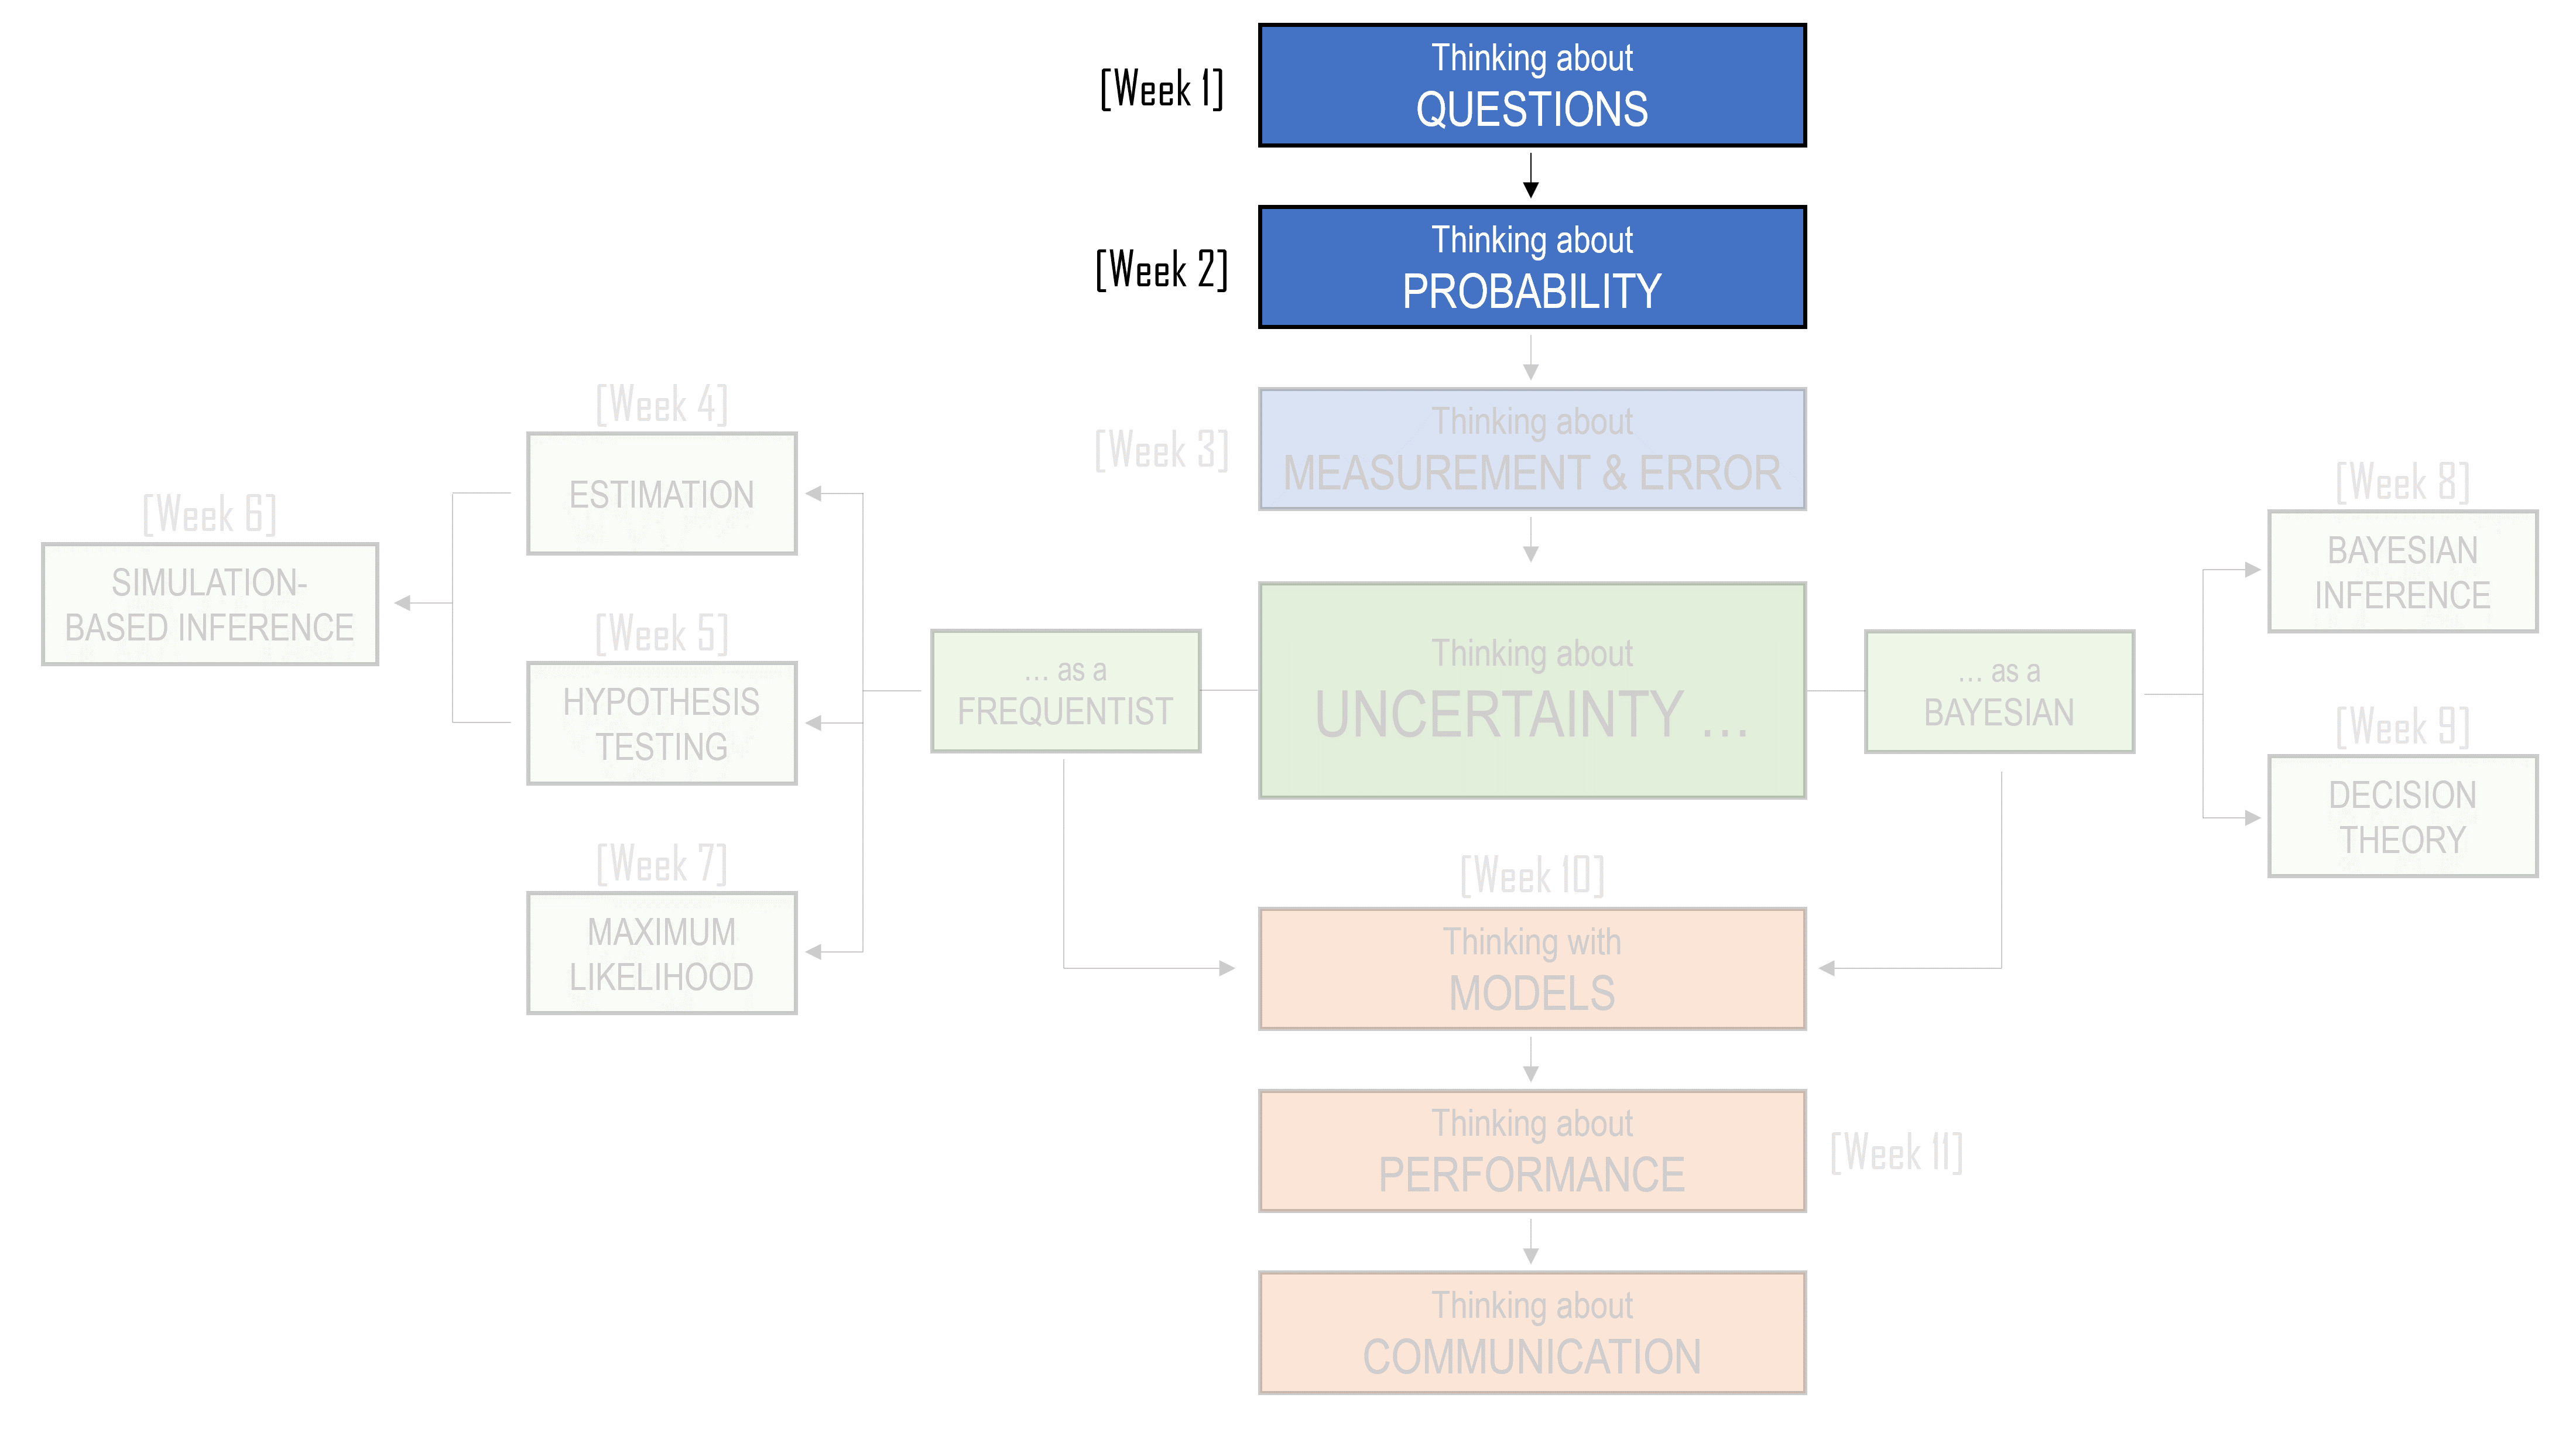
\includegraphics[width=14.81in,height=\textheight,keepaspectratio]{images/chapter2/outline.png}

\section{The problem with intuition}\label{the-problem-with-intuition}

\emph{Parade} magazine had been part of American popular culture for
decades. It began publication in 1941 and, for much of its life, was
distributed as a Sunday newspaper magazine. At its peak, it reached
millions of readers each week. Although the print magazine eventually
ceased regular publication in 2022, \emph{Parade} continues today as a
website and email newsletter.

One of its most popular features was the ``Ask Marilyn'' column, which
began in 1986. The column was written by Marilyn vos Savant, who became
well known for answering puzzles, logic problems, and questions from
readers. People wrote to her about all kinds of things: mathematics,
language, philosophy, everyday reasoning, and strange little problems
that seemed simple at first but became more difficult the longer one
thought about them.

\pandocbounded{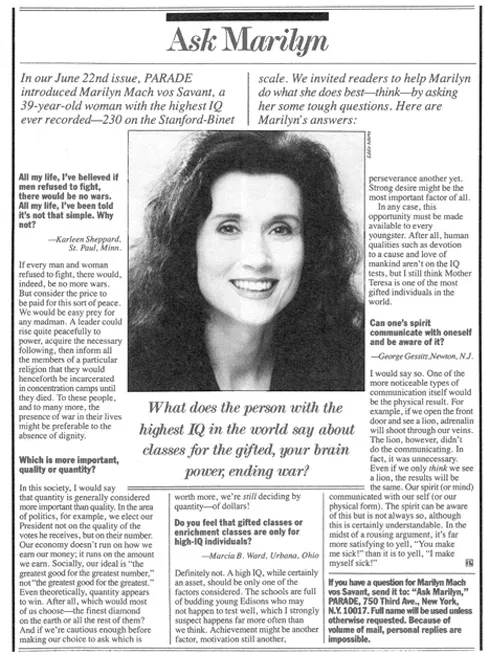
\includegraphics[keepaspectratio]{images/chapter2/askmarilyn.png}}

Perhaps the most famous question Marilyn ever answered was about a game
show. It is now famously referred to as \emph{The Monty Hall Problem},
and has appeared in modern television shows such as \emph{NUMB3RS},
\emph{Brooklyn Nine-Nine}, \emph{Mythbusters}, and the 2008 movie
\emph{21}.

\subsection{The Monty Hall Problem}\label{the-monty-hall-problem}

In the puzzle, you are a contestant on a game show.

\begin{itemize}
\tightlist
\item
  In front of you are three closed doors.

  \begin{itemize}
  \tightlist
  \item
    Behind one door is a car.
  \item
    Behind the other two doors are goats.
  \end{itemize}
\item
  You choose one door.

  \begin{itemize}
  \tightlist
  \item
    The host, who knows what is behind each door, then opens one of the
    two doors you did not choose.
  \item
    The door he opens has a goat behind it.
  \end{itemize}
\item
  There are now two unopened doors: the door you originally chose, and
  one other door.
\item
  The host gives you a choice:
\end{itemize}

\begin{quote}
Should you stay with your original door, or should you switch?
\end{quote}

\pandocbounded{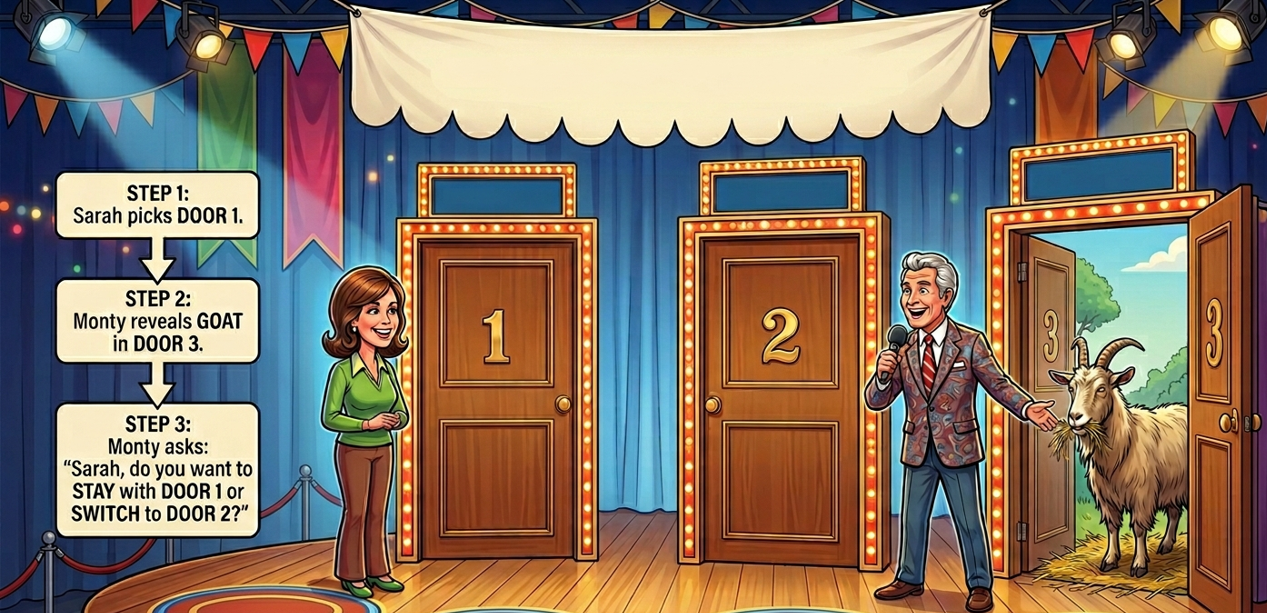
\includegraphics[keepaspectratio]{images/chapter2/montyhall.png}}

At first, the answer seems obvious. There are two doors left. One has a
car, and one has a goat. So it feels like the probability must now be
50/50. If there are only two possibilities, surely each is equally
likely?

This is a good moment to pause and ask yourself what you would do.

\begin{itemize}
\tightlist
\item
  Would you stay?
\item
  Would you switch?
\item
  Would you say it does not matter?
\end{itemize}

\begin{tcolorbox}[enhanced jigsaw, arc=.35mm, bottomrule=.15mm, bottomtitle=1mm, breakable, colback=white, colbacktitle=quarto-callout-note-color!10!white, colframe=quarto-callout-note-color-frame, coltitle=black, left=2mm, leftrule=.75mm, opacityback=0, opacitybacktitle=0.6, rightrule=.15mm, title=\textcolor{quarto-callout-note-color}{\faInfo}\hspace{0.5em}{Click to see what Mariln suggests you should do}, titlerule=0mm, toprule=.15mm, toptitle=1mm]

Marilyn's answer was that: you should switch.

\end{tcolorbox}

This answer caused an enormous backlash. Many readers (over 10,000
letters, including nearly 1000 PhDs) wrote in to say she was wrong. Some
of the responses were not simply polite disagreements. People were
confident that the answer had to be 50/50, and many were amazed that
someone known for solving logic puzzles would make what they saw as such
an obvious mistake.

A Mathematics Professor from George Mason University wrote:

\begin{quote}
``You blew it! Let me explain. If one door is shown to be a loser, that
information changes the probability of either remaining choice, neither
of which has any reason to be more likely to 1/2. As a professional
mathematician, I'm very concerned with the general public's lack of
mathematical skills. Please help by confessing your error and in the
future being more careful.''
\end{quote}

From Dickinson State University:

\begin{quote}
``I am in shock that after being corrected by at least three
mathematicians, you still do not see your mistake.''
\end{quote}

From Georgetown:

\begin{quote}
``How many irate mathematicians are needed to change your mind?''
\end{quote}

But \ldots{} Marilyn's answer was the correct one. Switching gives you a
better chance of winning the car.

The Monty Hall problem has since become one of the most famous examples
in probability. Part of its appeal is that it does not require advanced
mathematics. You do not need calculus, algebra, or specialised
statistical theory to solve it. What you need is a careful understanding
of how probability works, and especially how to define the set of
possible outcomes.

This is where intuition can mislead us. We look at the final situation:
two unopened doors, and our mind jumps to ``50/50''. But here is the
important part:

\begin{quote}
Probability is not only about counting what we can see at the end. It is
about understanding the full process that produced the situation we are
in.
\end{quote}

For now, we will leave the puzzle unresolved. Instead of jumping
straight to the answer, we will use the Monty Hall problem as a reason
to build up the basic language of probability. We will begin with
outcomes, events, and sample spaces. Then we will use these ideas to
return to the Monty Hall problem and see whether our first intuition
still holds.

\section{Cardano and the law of the sample
space}\label{cardano-and-the-law-of-the-sample-space}

Long before Marilyn vos Savant received angry letters about the Monty
Hall problem, people were already arguing, guessing, and reasoning badly
about games of chance. One of the earliest people to think carefully
about these questions was Gerolamo Cardano.

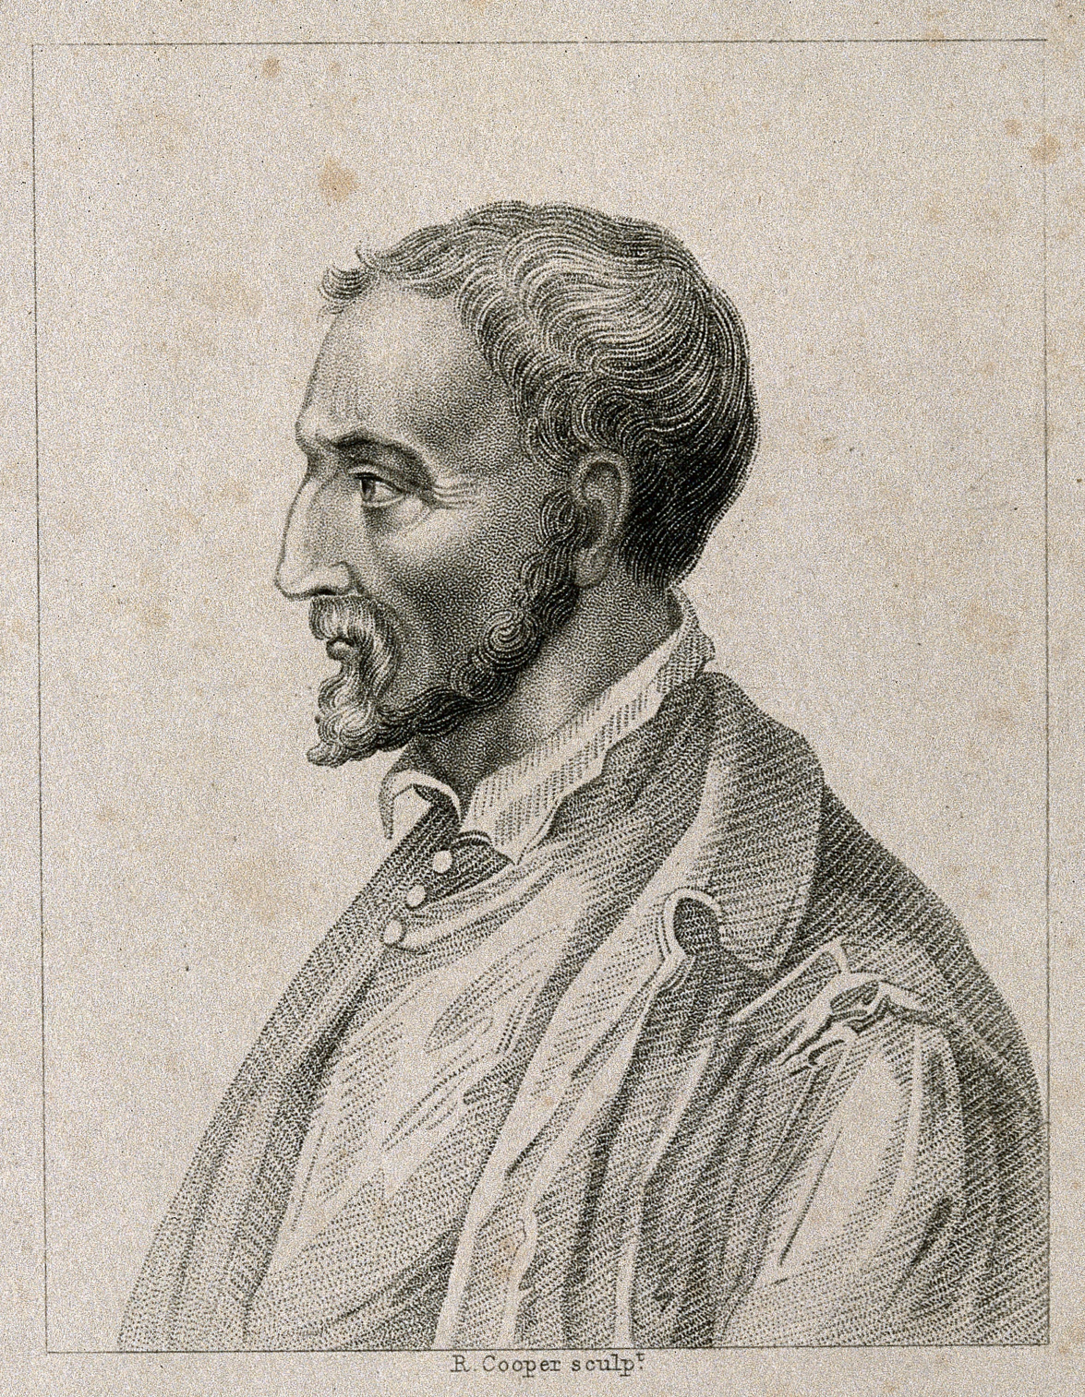
\includegraphics[width=0.5\linewidth,height=\textheight,keepaspectratio]{images/chapter2/cardano.png}

\textbf{17th-century portrait engraving of Cardano}

Cardano was born in Milan in 1501. His early life was difficult. He was
an illegitimate child, he grew up in an unstable household, and his
health was often poor. Yet he became one of the most remarkable thinkers
of the Renaissance: a physician, mathematician, astrologer, inventor,
and writer. He was brilliant, difficult, restless, and often unlucky.

He was also a gambler.

From a young age, Cardano noticed that he had a talent for games of
chance. In his time, gambling was common. People played games involving
dice, cards, coins, and objects known as \emph{astrali}, which were
small bones or dice-like objects used in games of chance. Gambling was
not merely entertainment. For many people, including Cardano, it was
also a way to make money, lose money, test one's nerve, and attempt to
understand fortune.

Cardano's interest in gambling eventually led him to write a book called
\emph{Liber de Ludo Aleae}, usually translated as \emph{The Book on
Games of Chance}. It is often described as one of the first serious
attempts in history to understand uncertainty mathematically. Cardano
was not writing probability in the modern language we use today, but he
was beginning to express one of its central ideas: to reason well about
chance, we must first understand all the possible outcomes.

One of the chapters in Cardano's book was titled ``On Combined Points'',
or ``On Possibilities''. In that chapter, Cardano described what he
called a ``general rule''. In modern terms, this rule is closely related
to what we now call the law of the sample space.

The idea is simple, but powerful:

\begin{quote}
If all outcomes are equally likely, the probability of an event is the
number of outcomes in which the event occurs divided by the total number
of possible outcomes.
\end{quote}

This is one of the foundations of probability.

But the simplicity is deceptive. Many probability mistakes happen
because we do not define the possible outcomes carefully enough.

\begin{tcolorbox}[enhanced jigsaw, arc=.35mm, bottomrule=.15mm, bottomtitle=1mm, breakable, colback=white, colbacktitle=quarto-callout-note-color!10!white, colframe=quarto-callout-note-color-frame, coltitle=black, left=2mm, leftrule=.75mm, opacityback=0, opacitybacktitle=0.6, rightrule=.15mm, title=\textcolor{quarto-callout-note-color}{\faInfo}\hspace{0.5em}{Some terminology}, titlerule=0mm, toprule=.15mm, toptitle=1mm]

A \textbf{sample space} is the set of all possible outcomes of a random
process.

If we roll a standard six-sided die, the sample space is:

\[
S = \{1,2,3,4,5,6\}.
\]

Each number in this set is an \textbf{outcome}. An outcome is one
possible result of the random process.

An \textbf{event} is a collection of outcomes. For example:

\begin{itemize}
\tightlist
\item
  The event ``roll an even number'' is: \(\{2,4,6\}\)
\item
  The event ``roll a number greater than 4'' is: \(\{5,6\}\)
\end{itemize}

If the die is fair, each of the six outcomes is equally likely. So the
probability of

\begin{itemize}
\tightlist
\item
  rolling a 4 is: \(P(4) = \frac{1}{6}\)
\item
  rolling an even number is:
  \(P(\text{even}) = \frac{3}{6} = \frac{1}{2}\)
\end{itemize}

This is Cardano's general rule in modern form. First, define the set of
possible outcomes. Then count the outcomes that match the event you care
about.

We can also see one of the basic rules, or axioms, of probability here.

Probabilities must be between 0 and 1:

\[
0 \leq P(A) \leq 1.
\]

An event with probability 0 is impossible. An event with probability 1
is certain. Most events we care about fall somewhere between these two
extremes.

For the die, rolling a 7 has probability 0, because 7 is not in the
sample space:

\[
P(7)=0.
\]

Rolling a number from 1 to 6 has probability 1, because one of those
outcomes must happen:

\[
P(\{1,2,3,4,5,6\})=1.
\]

This gives us another axiom of probability:

\[
P(S)=1.
\]

The probability of the entire sample space is 1. Something in the sample
space must happen.

\end{tcolorbox}

\subsection{The two-daughter problem}\label{the-two-daughter-problem}

Suppose a family has two children, and suppose, for simplicity, that
each child is equally likely to be a boy or a girl. Also suppose that
the sex of one child does not affect the sex of the other.

If we record the children in birth order, the sample space is:

\[
S = \{BB, BG, GB, GG\}.
\]

Here, \(BG\) means the older child is a boy and the younger child is a
girl. \(GB\) means the older child is a girl and the younger child is a
boy.

This distinction is important. If we ask, ``What is the probability that
both children are girls?'', the answer is:

\[
P(GG) = \frac{1}{4}.
\]

There is one outcome in which both children are girls, out of four
equally likely outcomes.

Now consider a slightly different question:

\begin{quote}
A family has two children. At least one of them is a girl. What is the
probability that both children are girls?
\end{quote}

Many people are tempted to reason like this: we already know one child
is a girl, so there is only one child left to consider. That remaining
child is either a boy or a girl, so the probability that both children
are girls must be \(1/2\).

This sounds reasonable, but it is not correct under the usual
assumptions of the problem. The mistake is that the sample space has
changed, but not in the way our intuition first suggests. Before
receiving any information, the sample space was:

\[
S = \{BB, BG, GB, GG\}.
\]

Once we are told that at least one child is a girl, the outcome \(BB\)
is no longer possible. So the reduced sample space is:

\[
S = \{BG, GB, GG\}.
\]

Of these three possible outcomes, only one has two girls:

\[
GG.
\]

So the probability is:

\[
P(\text{both girls} \mid \text{at least one girl}) = \frac{1}{3}.
\]

This is exactly the kind of situation Cardano's general rule helps us
handle. Instead of relying on intuition, we define the possible outcomes
and count them carefully.

\subsection{Why the wording matters}\label{why-the-wording-matters}

Probability problems are often sensitive to how information is obtained.

Compare the previous question with this one:

\begin{quote}
A family has two children. The older child is a girl. What is the
probability that both children are girls?
\end{quote}

Now the sample space is different again.

If the older child is known to be a girl, then the only possible
outcomes are:

\[
S = \{GB, GG\}.
\]

Only one of these outcomes has two girls, so:

\[
P(\text{both girls} \mid \text{older child is a girl}) = \frac{1}{2}.
\]

The difference between these two questions is subtle but important. ``At
least one child is a girl'' and ``the older child is a girl'' sound
similar, but they give different information. Different information
means a different sample space. A different sample space can mean a
different probability.

This is one of the central lessons of probability:

\begin{quote}
To solve a probability problem, we must know not only what happened, but
how we came to know it.
\end{quote}

\section{Solving Monty Hall with the sample
space}\label{solving-monty-hall-with-the-sample-space}

We are now in a better position to think about the Monty Hall problem
that was introduced at the start of this chapter.

At the beginning of the game, there are three possible locations for the
car:

\[
S = \{\text{Door 1}, \text{Door 2}, \text{Door 3}\}.
\]

If you choose Door 1, then the chance that your first choice is correct
is \(1/3\). The chance that the car is behind one of the two doors you
did not choose is \(2/3\).

This part is straightforward. The sample space has three equally likely
possibilities.

The difficult part comes after the host opens a door. Many people look
at the two remaining closed doors and think the sample space must now
be:

\[
S = \{\text{your door}, \text{other unopened door}\}.
\]

If those two possibilities were equally likely, the answer would be
\(1/2\). But we have just seen that we must be careful. The correct
sample space depends not only on what remains visible, but on how the
information was produced.

In the Monty Hall problem, the host knows where the car is. The host
does not open a door randomly. The host deliberately opens a door with a
goat behind it. That means the host's action carries information.

Suppose, without loss of generality, that you first choose Door 1. There
is nothing special about Door 1. We are choosing it only so that we can
write down the possible outcomes clearly.

At the moment you choose Door 1, the car could be behind Door 1, Door 2,
or Door 3.

\[
S = \{\text{Car behind Door 1}, \text{Car behind Door 2}, \text{Car behind Door 3}\}.
\]

Each of these possibilities has probability \(1/3\).

Now consider what happens in each case.

{\def\LTcaptype{none} % do not increment counter
\begin{longtable}[]{@{}
  >{\raggedright\arraybackslash}p{(\linewidth - 8\tabcolsep) * \real{0.2000}}
  >{\raggedright\arraybackslash}p{(\linewidth - 8\tabcolsep) * \real{0.2000}}
  >{\raggedright\arraybackslash}p{(\linewidth - 8\tabcolsep) * \real{0.2000}}
  >{\raggedright\arraybackslash}p{(\linewidth - 8\tabcolsep) * \real{0.2000}}
  >{\raggedright\arraybackslash}p{(\linewidth - 8\tabcolsep) * \real{0.2000}}@{}}
\toprule\noalign{}
\begin{minipage}[b]{\linewidth}\raggedright
Where the car is
\end{minipage} & \begin{minipage}[b]{\linewidth}\raggedright
Your first choice
\end{minipage} & \begin{minipage}[b]{\linewidth}\raggedright
What the host can open
\end{minipage} & \begin{minipage}[b]{\linewidth}\raggedright
If you stay
\end{minipage} & \begin{minipage}[b]{\linewidth}\raggedright
If you switch
\end{minipage} \\
\midrule\noalign{}
\endhead
\bottomrule\noalign{}
\endlastfoot
Door 1 & Door 1 & Door 2 or Door 3 & Win & Lose \\
Door 2 & Door 1 & Door 3 & Lose & Win \\
Door 3 & Door 1 & Door 2 & Lose & Win \\
\end{longtable}
}

This table is the key to the problem.

If the car is behind Door 1, then your first choice was correct. The
host can open either Door 2 or Door 3, because both of those doors have
goats behind them. If you stay, you win. If you switch, you lose.

If the car is behind Door 2, then your first choice was wrong. The host
cannot open Door 2, because that would reveal the car. The host must
open Door 3, revealing a goat. If you stay, you lose. If you switch, you
win.

If the car is behind Door 3, then your first choice was wrong. The host
must open Door 2. If you stay, you lose. If you switch, you win.

So switching wins in two of the three possible cases.

\[
P(\text{win by switching}) = \frac{2}{3}.
\]

Staying wins in only one of the three possible cases.

\[
P(\text{win by staying}) = \frac{1}{3}.
\]

This is why Marilyn vos Savant was right. You should switch.

The most important point is that the host's action does not reset the
probabilities to \(1/2\) and \(1/2\). Your original choice had a \(1/3\)
chance of being correct when you made it. The host's action does not
change the fact that your first choice was probably wrong. In fact, your
first choice was wrong with probability \(2/3\).

\begin{tcolorbox}[enhanced jigsaw, arc=.35mm, bottomrule=.15mm, bottomtitle=1mm, breakable, colback=white, colbacktitle=quarto-callout-note-color!10!white, colframe=quarto-callout-note-color-frame, coltitle=black, left=2mm, leftrule=.75mm, opacityback=0, opacitybacktitle=0.6, rightrule=.15mm, title=\textcolor{quarto-callout-note-color}{\faInfo}\hspace{0.5em}{Bonus Round}, titlerule=0mm, toprule=.15mm, toptitle=1mm]

Imagine you were playing a variation of the Monty Hall game, except the
rules are now:

\begin{enumerate}
\def\labelenumi{\arabic{enumi}.}
\tightlist
\item
  There are 100 doors
\item
  Behind one of these doors is a car
\item
  Behind the other 99 doors are goats
\item
  You choose 1 door
\item
  The host (who knows there the car is), opens 98 doors that you did not
  choose, each revealing a goat.
\item
  There are now 2 doors left: 1 with a car, and 1 with a goat
\item
  The host asks you:
\end{enumerate}

\begin{quote}
``Do you stay or switch?''
\end{quote}

Using the same logic as above, can you determine the best choice to make
here?

\end{tcolorbox}

The idea of the sample space gives us a way to begin thinking carefully
about probability. Before we can assign probabilities, we need to know
what the possible outcomes are.

But there is another important step. Once we know the possible outcomes,
we often need to ask:

\begin{quote}
How many different ways can the event happen?
\end{quote}

\section{Galileo and counting the ways something can
happen}\label{galileo-and-counting-the-ways-something-can-happen}

The Monty Hall problem shows why the sample space matters. At first, we
see two unopened doors and our intuition says ``two possibilities, so
50/50''. But once we carefully describe the full process (i.e., your
original choice, the host's knowledge, and the door the host is forced
to open) we see that the two remaining doors do not have the same
probability. The lesson is not just that we need to list the possible
outcomes. We also need to count them in the right way.

This brings us to the next step in probability thinking. Sometimes the
difficulty is not deciding what the outcomes are, but recognising that
an event can happen in more than one way. Two events may look equally
likely on the surface, but one may have more hidden pathways leading to
it. This takes us to the yea 1583, where we meet a young Galileo
Galilei.

Today, Galileo Galilei is remembered as one of the great figures in the
history of science. He is best known for his work in astronomy and
physics, including his telescopic observations, his studies of motion,
and his role in the controversy with the Church.

\pandocbounded{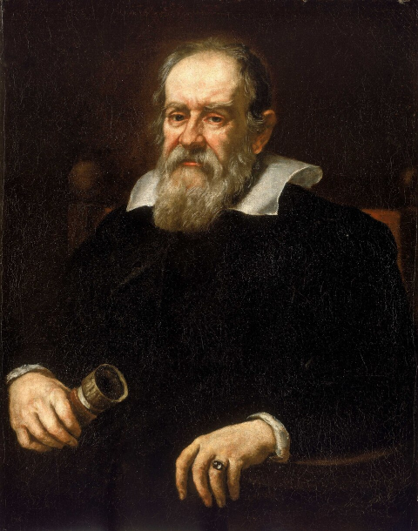
\includegraphics[keepaspectratio]{images/chapter2/Galileo.png}}

However, Galileo also made a rather unusual contribution to the early
understanding of probability. While connected with the University of
Pisa, Galileo was hired by the Grand Duke of Tuscany to explain a
problem involving dice:

\begin{quote}
When you throw three dice, why does the sum of 10 appear more frequently
than the sum of 9?
\end{quote}

At first, this seems strange. There are six combinations that can
produce a total of 9:

\[
1+2+6 = 9
\]

\[
1+3+5 = 9
\]

\[
1+4+4 = 9
\]

\[
2+2+5 = 9
\]

\[
2+3+4 = 9
\]

\[
3+3+3 = 9
\]

There are also six combinations that can produce a total of 10:

\[
1+3+6 = 10
\]

\[
1+4+5 = 10
\]

\[
2+2+6 = 10
\]

\[
2+3+5 = 10
\]

\[
2+4+4 = 10
\]

\[
3+3+4 = 10
\]

So it seems as though 9 and 10 should be equally likely. However, the
Grand Duke had noticed that 10 appeared more often. Galileo explained
why. The mistake is that the lists above do not count all the possible
ways the dice can land. They count combinations, but they do not count
order.

For example:

\[
1+2+6
\]

can occur in several different ways:

\[
(1,2,6)
\]

\[
(1,6,2)
\]

\[
(2,1,6)
\]

\[
(2,6,1)
\]

\[
(6,1,2)
\]

\[
(6,2,1)
\]

These are different outcomes when three dice are rolled, because the
first die, second die, and third die can each show different numbers.

So although 9 and 10 each appear to have six combinations, those
combinations do not produce the same number of ordered outcomes.

For a total of 9, there are 25 ordered outcomes.

For a total of 10, there are 27 ordered outcomes.

Therefore:

\[
P(\text{sum is 9}) = \frac{25}{216}
\]

while

\[
P(\text{sum is 10}) = \frac{27}{216}.
\]

A total of 10 is slightly more likely.

The difference is small, but gamblers who played often enough (such as
the Grand Duke) could notice it. Galileo's contribution was to show that
the pattern was not magic, luck, or superstition. It came from counting
the possible outcomes properly.

This gives us another important rule:

\begin{quote}
The probability of an event depends on the number of ways in which it
can occur.
\end{quote}

\subsection{The birthday problem}\label{the-birthday-problem}

One of the most famous examples of counting the ways an event can happen
is the birthday problem. Imagine a class of students. Ignore leap years
and assume that each birthday is equally likely to fall on any of the
365 days of the year. Here is the question:

\begin{quote}
How many people need to be in a room before there is a better than 50\%
chance that at least two people share a birthday?
\end{quote}

Most people guess a number much larger than the true answer. There are
365 possible birthdays, so it feels as though we would need a very large
group before a shared birthday becomes likely. Many people guess 100,
150, or even more.

\begin{tcolorbox}[enhanced jigsaw, arc=.35mm, bottomrule=.15mm, bottomtitle=1mm, breakable, colback=white, colbacktitle=quarto-callout-note-color!10!white, colframe=quarto-callout-note-color-frame, coltitle=black, left=2mm, leftrule=.75mm, opacityback=0, opacitybacktitle=0.6, rightrule=.15mm, title=\textcolor{quarto-callout-note-color}{\faInfo}\hspace{0.5em}{Click to see answer}, titlerule=0mm, toprule=.15mm, toptitle=1mm]

The surprising answer is 23.

With just 23 people, the probability that at least two people share a
birthday is slightly greater than 50\%.

\end{tcolorbox}

The easiest way to calculate the birthday problem is to work backwards.
Instead of first calculating the probability that at least two people
share a birthday, we calculate the probability that nobody shares a
birthday.

The first person can have any birthday, since there is no one else to
match with. The second person must avoid that first birthday, leaving
364 possible birthdays that would keep everyone unique. The third person
must avoid the two birthdays already taken, leaving 363 possible
choices. The fourth person must avoid three birthdays, leaving 362
possible choices. Continuing this pattern, each new person has one fewer
safe birthday available than the person before them.

{\def\LTcaptype{none} % do not increment counter
\begin{longtable}[]{@{}
  >{\raggedright\arraybackslash}p{(\linewidth - 6\tabcolsep) * \real{0.1200}}
  >{\raggedright\arraybackslash}p{(\linewidth - 6\tabcolsep) * \real{0.4800}}
  >{\raggedright\arraybackslash}p{(\linewidth - 6\tabcolsep) * \real{0.2200}}
  >{\raggedright\arraybackslash}p{(\linewidth - 6\tabcolsep) * \real{0.1800}}@{}}
\toprule\noalign{}
\begin{minipage}[b]{\linewidth}\raggedright
Person
\end{minipage} & \begin{minipage}[b]{\linewidth}\raggedright
What must happen
\end{minipage} & \begin{minipage}[b]{\linewidth}\raggedright
Safe birthday choices
\end{minipage} & \begin{minipage}[b]{\linewidth}\raggedright
Probability
\end{minipage} \\
\midrule\noalign{}
\endhead
\bottomrule\noalign{}
\endlastfoot
1st person & Can have any birthday & 365 & \(\frac{365}{365}\) \\
2nd person & Must avoid the first person's birthday & 364 &
\(\frac{364}{365}\) \\
3rd person & Must avoid the first two birthdays & 363 &
\(\frac{363}{365}\) \\
4th person & Must avoid the first three birthdays & 362 &
\(\frac{362}{365}\) \\
\ldots{} & Continue in the same way & \ldots{} & \(\cdots\) \\
23rd person & Must avoid the birthdays of the first 22 people & 343 &
\(\frac{343}{365}\) \\
\end{longtable}
}

Multiplying these probabilities together, for 23 people the probability
that nobody shares a birthday is:

\[
\frac{365}{365}
\times
\frac{364}{365}
\times
\frac{363}{365}
\times
\cdots
\times
\frac{343}{365}
\approx 0.493.
\]

Notice that the probability we have just calculated is \textbf{not} the
probability that someone shares a birthday. We have calculated the
probability that nobody shares a birthday.

We can now apply the \textbf{complement rule} to solve this.

The \textbf{complement rule} says that if an event has probability
(P(A)), then the probability that the event does \textbf{not} happen is:

\[
P(\text{not } A) = 1 - P(A).
\]

Equivalently,

\[
P(A) = 1 - P(\text{not } A).
\]

In the birthday problem, let (A) be the event that \textbf{at least two
people share a birthday}.

Then the complement of (A), written (A\^{}c), is the event that
\textbf{nobody shares a birthday}.

So:

\[
A = \text{at least two people share a birthday}
\]

and

\[
A^c = \text{nobody shares a birthday}.
\]

These two events cover all possible outcomes. Either there is at least
one shared birthday, or there is no shared birthday. Since one of these
must happen, their probabilities add to 1:

\[
P(A) + P(A^c) = 1.
\]

Rearranging this gives:

\[
P(A) = 1 - P(A^c).
\]

In this example, we calculated:

\[
P(A^c) = P(\text{nobody shares a birthday}) \approx 0.493.
\]

Therefore:

\[
P(A)
=
1 - P(A^c)
=
1 - 0.493
=
0.507.
\]

So the probability that at least two people share a birthday is
approximately (0.507), or \textbf{50.7\%}.

In the birthday problem, it is easier to calculate the probability of no
shared birthdays and then subtract from 1. This is a common strategy in
probability. When the event we care about is hard to count directly, it
may be easier to count its complement.

\begin{quote}
The birthday problem is surprising because a shared birthday feels
unlikely when we think about one comparison at a time. But it becomes
much more likely when we count all the possible comparisons. This is one
reason probability often feels unintuitive. Our minds tend to focus on
one person, one comparison, or one outcome. Probability often asks us to
step back and count the whole structure of possibilities.
\end{quote}

\section{Pascal, Fermat, and the mathematics of
chance}\label{pascal-fermat-and-the-mathematics-of-chance}

Galileo's work with dice showed that probability depends on counting the
ways an event can happen. Some outcomes are more likely than others, not
because they are favoured by fate, but because there are more ways for
them to occur.

This idea also helps explain events that look astonishing at first
glance. In Germany's Lotto 6/49, six winning numbers are drawn from the
numbers 1 to 49. On June 21, 1995, the winning numbers were:

\[
15,\ 25,\ 27,\ 30,\ 42,\ 48.
\]

What made this draw remarkable was that the exact same set of numbers
had already appeared on December 20, 1986. It was the first repeated
winning sequence in 3,016 drawings.

At first, this sounds almost impossible. But, as with the birthday
problem, the important question is not just

\begin{quote}
``What is the chance of this exact sequence appearing again?''
\end{quote}

A better question is

\begin{quote}
``Across thousands of drawings, how many opportunities were there for
some sequence to repeat?''
\end{quote}

But how do we actually calculate a probability like this? (by the way,
the answer is 28\% - a value we'll learn how to compute later). The
numbers are too large to list every possible lottery draw, and the event
we care about is not just one specific repeat. We want to know the
chance that any repeat occurs somewhere among thousands of draws.

This is where the work of Blaise Pascal and Pierre de Fermat becomes
important. Pascal is remembered for many contributions to mathematics
and science, including Pascal's triangle, work on pressure and fluids,
and his writing on philosophy and religion. Fermat is best known for his
work in number theory, including the famous Fermat's Last Theorem, as
well as important ideas in analytic geometry and calculus.

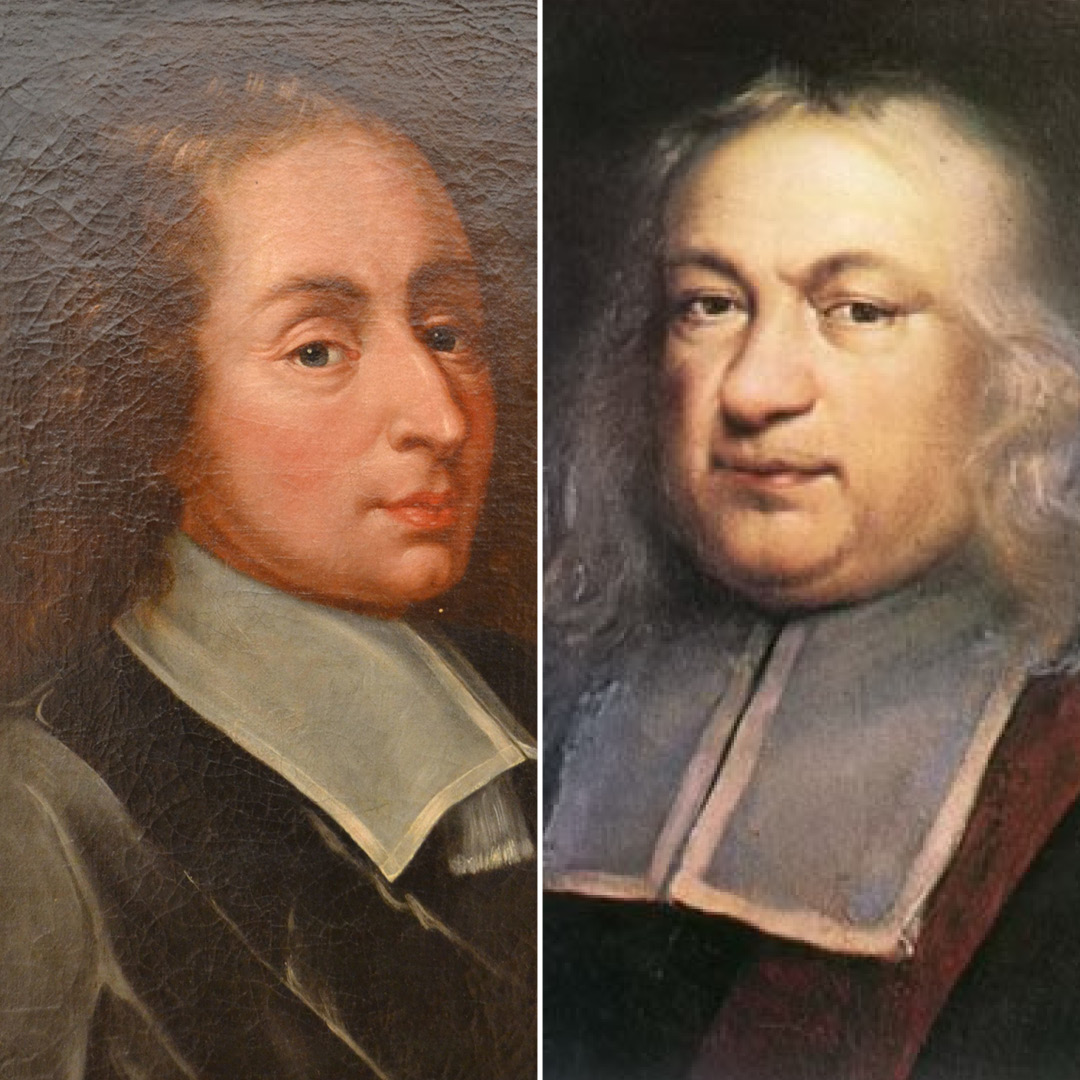
\includegraphics[width=0.5\linewidth,height=\textheight,keepaspectratio]{images/chapter2/pascal_and_fermat.jpg}

However, in this section, we are interested in a famous correspondence
between the two of them about games of chance. In the seventeenth
century, Pascal and Fermat exchanged letters about how to solve problems
involving uncertainty, especially the question of how to divide the
stakes of an unfinished game fairly (i.e.~``\emph{The Problem of
Points}). These questions came from gambling, but the ideas behind them
became much more important. Their correspondence helped establish
probability as a mathematical subject: a way of counting possible
outcomes, comparing favourable cases with all cases, and reasoning
systematically about chance.

\begin{tcolorbox}[enhanced jigsaw, arc=.35mm, bottomrule=.15mm, bottomtitle=1mm, breakable, colback=white, colbacktitle=quarto-callout-note-color!10!white, colframe=quarto-callout-note-color-frame, coltitle=black, left=2mm, leftrule=.75mm, opacityback=0, opacitybacktitle=0.6, rightrule=.15mm, title=\textcolor{quarto-callout-note-color}{\faInfo}\hspace{0.5em}{The Problem of Points}, titlerule=0mm, toprule=.15mm, toptitle=1mm]

The Problem of Points goes something like this:

\begin{quote}
Imagine two players are playing a coin-flipping game. We will call them
Harry and Tom. Harry scores a point whenever the coin lands Heads (H).
Tom scores a point whenever the coin lands Tails (T). The first player
to reach 3 points wins the game and takes the prize of \$100. Now
suppose the first three flips are: H, T, H. So the current score is H =
2, and T = 1. Harry needs one more Head to win. Tom needs two more
Tails. Now imagine that, for some reason, the game is interrupted and
cannot continue. How should Harry and Tom divide the \$100 prize?
\end{quote}

One tempting answer is to divide the prize according to the current
score. Harry has 2 points and Tom has 1 point, so perhaps Harry should
receive two-thirds of the prize and Tom should receive one-third.

But this does not answer the \textbf{right question}.

The prize was not meant to reward whoever was ahead when the game
stopped. It was meant to reward whoever would eventually reach 3 points
first. So the fair question is not:

\begin{quote}
What is the score right now?
\end{quote}

The fair question is:

\begin{quote}
If the game had continued, what chance did each player have of winning?
\end{quote}

To solve this, let us consider all possible futures that the game could
have finished:

\pandocbounded{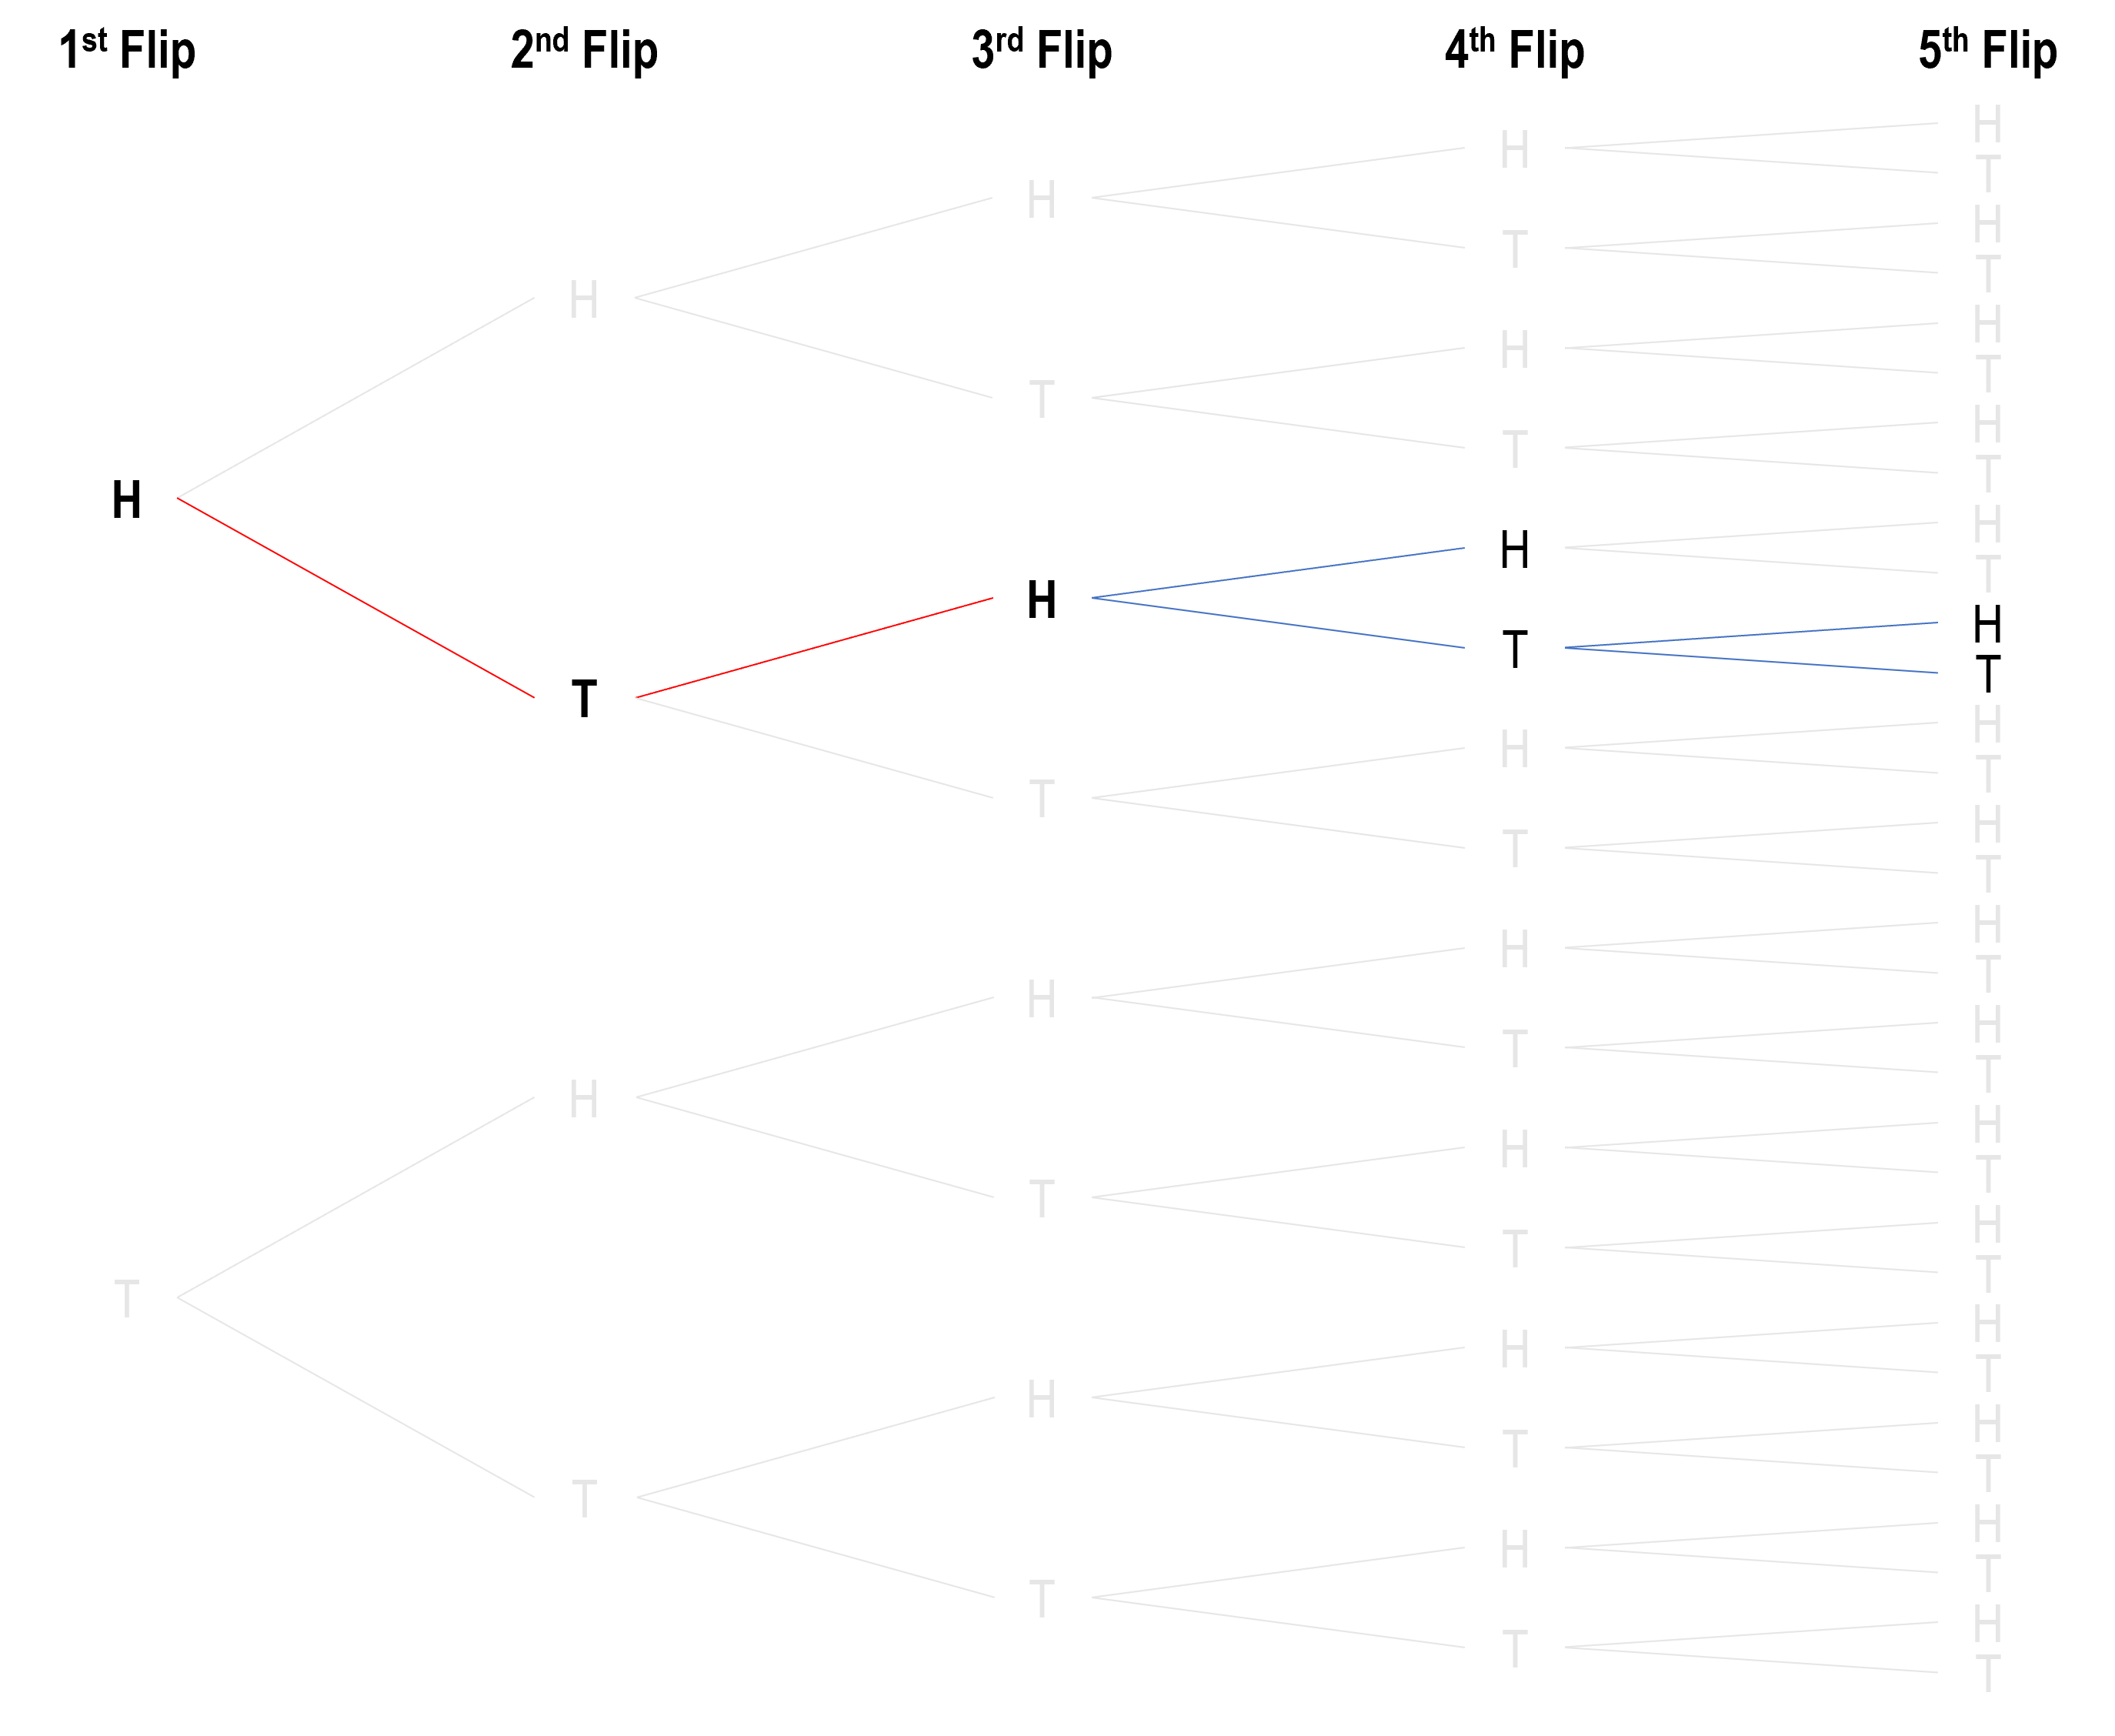
\includegraphics[keepaspectratio]{images/chapter2/problemofpoints.png}}

If the fourth flip is Heads, then Harry reaches 3 points, wins the
prize, and the game stops immediately. However, if the fourth flip is
Tails, the score becomes tied at 2 points each, and a fifth flip is
required to decide the winner.

So, from the interrupted position, the sample space of possible ways the
game can finish is:

\[
S = \{H,TH,TT\}
\]

This sample space needs to be treated carefully, because the outcomes
are not equally likely. The outcome (H) requires only one future flip,
while (TH) and (TT) require two future flips.

Therefore:

\[
P(H)=\frac{1}{2}
\]

\[
P(TH)=\frac{1}{2}\times\frac{1}{2}=\frac{1}{4}
\]

\[
P(TT)=\frac{1}{2}\times\frac{1}{2}=\frac{1}{4}
\]

\begin{table}
\fontsize{12.0pt}{14.0pt}\selectfont
\begin{tabular*}{\linewidth}{@{\extracolsep{\fill}}ccc}
\toprule
Future flips & Probability & Winner \\ 
\midrule\addlinespace[2.5pt]
H & 1/2 & Harry \\ 
TH & 1/4 & Harry \\ 
TT & 1/4 & Tom \\ 
\bottomrule
\end{tabular*}
\end{table}

Therefore, the probability of Harry winning is:

\[
\begin{aligned}
P(\text{Harry wins})
&= P(H) + P(TH) \
&= \frac{1}{2} + \frac{1}{4} \
&= \frac{3}{4}
\end{aligned}
\]

The probability of Tom winning is:

\[
\begin{aligned}
P(\text{Tom wins})
&= P(TT) \
&= \frac{1}{4}
\end{aligned}
\]

So the fair way to divide the \$100 prize is not according to the
current score of 2 to 1. Instead, it should be divided according to each
player's probability of eventually winning the game.

\begin{itemize}
\item
  Harry should receive: \(\frac{3}{4}\times 100 = \$75\)
\item
  Tom should receive: \(\frac{1}{4}\times 100 = \$25\)
\end{itemize}

This is the central idea behind the problem of points. The value of an
unfinished game is not determined only by the score at the moment the
game stops. It is determined by the possible futures that remain, and by
the probability of each of those futures.

It also reinforces a lesson from earlier in the chapter. A sample space
is not enough on its own. We must also ask whether the outcomes in the
sample space are equally likely. In this example, there are three
possible future paths, but Harry does not win with probability \(2/3\).
That would only be true if the three paths were equally likely. Since
\(P(H)\) is more likely than either \(P(TH)\) or \(P(TT)\), the correct
probability is \(3/4\).

\end{tcolorbox}

\subsection{Pascal's triangle and
combinations}\label{pascals-triangle-and-combinations}

The problem of points shows us how probability can be used to reason
about unfinished situations. But so far, our counting problems have been
small enough to carry out without much effort. As the numbers get
larger, counting becomes difficult. Suppose you are arranging a wedding
reception for 100 guests, and each table seats 10 people. Even if we
focus only on the first table, the question quickly becomes large:

\begin{quote}
How many ways are there to choose 10 people from a group of 100?
\end{quote}

This is a counting problem that appears in many other settings. It is
similar to asking how many ways there are to choose 10 investments from
100 possible funds, 10 applicants from 100 candidates, or 10 suburbs
from 100 possible sites for a policy trial.

The story changes, but the mathematical structure is the same. We are
choosing a group of 10 from a larger group of 100.

This is where we need to distinguish between an \textbf{arrangement} and
a \textbf{combination}.

\begin{itemize}
\tightlist
\item
  An arrangement counts different orders.
\item
  A combination counts different groups.
\end{itemize}

This distinction matters because probability depends on counting the
right thing.

Let us use a small example. Suppose there are 4 guests:

\[
A,B,C,D
\]

and we want to choose 2 of them. The possible pairs are:

\[
AB,\; AC,\; AD,\; BC,\; BD,\; CD
\]

There are 6 possible pairs. So the number of ways to choose 2 guests
from 4 is 6. We write this as:

\[
\binom{4}{2}=6
\]

and read it as ``4 choose 2''.

This notation means:

\begin{quote}
How many ways are there to choose 2 items from 4, when order does not
matter?
\end{quote}

Now suppose we wanted to choose 1 guest from 4. There are obviously 4
ways:

\[
\binom{4}{1}=4
\]

If we wanted to choose all 4 guests from 4, there is only 1 way:

\[
\binom{4}{4}=1
\]

If we wanted to choose no guests from 4, there is also only 1 way:

\[
\binom{4}{0}=1
\]

That last one may feel strange at first. But there is exactly one way to
choose nothing: choose nobody.

So for 4 guests, the numbers are:

\[
\binom{4}{0}=1
\]

\[
\binom{4}{1}=4
\]

\[
\binom{4}{2}=6
\]

\[
\binom{4}{3}=4
\]

\[
\binom{4}{4}=1
\]

Written in a row, this gives:

\[
1 \quad 4 \quad 6 \quad 4 \quad 1
\]

This row appears in \textbf{Pascal's triangle}. Pascal's triangle is a
pattern of numbers that begins like this:

\[
1
\]

\[
1 \quad 1
\]

\[
1 \quad 2 \quad 1
\]

\[
1 \quad 3 \quad 3 \quad 1
\]

\[
1 \quad 4 \quad 6 \quad 4 \quad 1
\]

\[
1 \quad 5 \quad 10 \quad 10 \quad 5 \quad 1
\]

Pascal's triangle gives us a compact way to count possibilities without
writing them all out. The same counting idea can be written as a
formula:

\[
\binom{n}{k}
=
\frac{n!}{k!(n-k)!}
\]

This means the number of ways to choose \(k\) items from \(n\) items,
when order does not matter. For example, the number of ways to choose 10
guests from 100 is:

\[
\binom{100}{10}
=
\frac{100!}{10!90!}
\]

This number is enormous (17,310,309,456,440). The important point is not
that we need to memorise it. The important point is that probability
often depends on counting possibilities that are far too numerous to
list by hand. Pascal's triangle helps us count possibilities. Pascal
also helped develop another idea: how to place a value on uncertain
outcomes. That idea is called \textbf{mathematical expectation}.

\subsection{Mathematical expectation}\label{mathematical-expectation}

The problem of points asked how a prize should be divided when a game is
interrupted. Pascal and Fermat's solution was to look forward. Instead
of asking only what had already happened, they asked what could still
happen, how likely those futures were, and what each future was worth.

This way of thinking leads naturally to mathematical expectation.

The basic idea is simple:

\begin{quote}
To value an uncertain situation, multiply each possible outcome by its
probability, then add the results.
\end{quote}

If a random quantity \(X\) can take values:

\[
x_1,\;x_2,\;x_3,\ldots,x_k
\]

with probabilities:

\[
p_1,\;p_2,\;p_3,\ldots,p_k
\]

then the expected value is:

\[
E(X)
=
p_1x_1+p_2x_2+p_3x_3+\cdots+p_kx_k
\]

Expected value is not necessarily what will happen. It is not a
prediction of the next outcome. Instead, it is a long-run average, or a
way of placing a value on uncertainty before the outcome is known.

Expected value is easiest to understand through a simple game. Suppose
you pay \$10 to play a game in which a fair coin is tossed. If the coin
lands heads, you receive \$30. If it lands tails, you receive nothing.

\begin{table}
\fontsize{12.0pt}{14.0pt}\selectfont
\begin{tabular*}{\linewidth}{@{\extracolsep{\fill}}lcr}
\toprule
Outcome & Probability & Winnings \\ 
\midrule\addlinespace[2.5pt]
Heads & 1/2 & \$30 \\ 
Tails & 1/2 & \$0 \\ 
\bottomrule
\end{tabular*}
\end{table}

To calculate the expected winnings, we multiply each possible outcome by
its probability and then add the results:

\[
\begin{aligned}
E(\text{winnings})
&=
\left(\frac{1}{2}\times 30\right)
+
\left(\frac{1}{2}\times 0\right) \\
&= 15
\end{aligned}
\]

So the game pays, on average, \$15. However, it costs \$10 to play, so
the expected profit is:

\[
15 - 10 = 5
\]

This game has a positive expected value. That does not mean you will win
\$5 every time you play. In any single game, you either receive \$30 or
receive nothing. But over many repeated plays, the average profit would
tend towards \$5 per game.

Now change the game slightly. Suppose it still costs \$10 to play, and
the coin is still fair, but the prize for heads is now only \$15.

\begin{table}
\fontsize{12.0pt}{14.0pt}\selectfont
\begin{tabular*}{\linewidth}{@{\extracolsep{\fill}}lcr}
\toprule
Outcome & Probability & Winnings \\ 
\midrule\addlinespace[2.5pt]
Heads & 1/2 & \$15 \\ 
Tails & 1/2 & \$0 \\ 
\bottomrule
\end{tabular*}
\end{table}

The expected winnings are now:

\[
\begin{aligned}
E(\text{winnings})
&=
\left(\frac{1}{2}\times 15\right)
+
\left(\frac{1}{2}\times 0\right) \\
&= 7.50
\end{aligned}
\]

Since the game still costs \$10 to play, the expected profit is:

\[
7.50 - 10 = -2.50
\]

This game has a negative expected value. You might still win if you play
once, but the structure of the game works against you in the long run.

The important lesson is this:

\begin{quote}
A game can be possible to win and still be a bad bet.
\end{quote}

\begin{tcolorbox}[enhanced jigsaw, arc=.35mm, bottomrule=.15mm, bottomtitle=1mm, breakable, colback=white, colbacktitle=quarto-callout-note-color!10!white, colframe=quarto-callout-note-color-frame, coltitle=black, left=2mm, leftrule=.75mm, opacityback=0, opacitybacktitle=0.6, rightrule=.15mm, title=\textcolor{quarto-callout-note-color}{\faInfo}\hspace{0.5em}{Everyday expectation}, titlerule=0mm, toprule=.15mm, toptitle=1mm]

Expected value can make ordinary decisions look different.

For example, my colleagues and I sometimes have different views about
parking on campus. Parking legally using the O-Park app costs about
\$5.50 per day. That is the certain cost: if you pay for parking, you
know exactly what you are giving up.

But suppose someone decides not to pay. On that particular day, parking
costs them nothing. Of course, they also run the risk of receiving a
parking fine. Suppose the fine is about \$125, and suppose the
probability of being fined on any given day is about:

\[
\frac{1}{20}
\]

We will discuss how to estimate probabilities like this from data in a
later chapter. For now, treat it as an assumption.

The choice can be summarised like this:

\begin{table}
\fontsize{12.0pt}{14.0pt}\selectfont
\begin{tabular*}{\linewidth}{@{\extracolsep{\fill}}lrrcr}
\toprule
Choice & Certain cost & Possible fine & Probability of fine & Expected cost \\ 
\midrule\addlinespace[2.5pt]
Pay using O-Park & \$5.50 & \$0 & 0 & \$5.50 \\ 
Do not pay & \$0 & \$125 & 1/20 & \$6.25 \\ 
\bottomrule
\end{tabular*}
\end{table}

If you pay through O-Park, the cost is simply:

\[
5.50
\]

If you do not pay, the expected cost is:

\[
\begin{aligned}
E(\text{fine})
&=
P(\text{fine})\times(\text{fine amount}) \
&=
\frac{1}{20}\times 125 \
&=
6.25
\end{aligned}
\]

So even though not paying feels cheaper on most individual days, its
expected cost is \$6.25 per day. That is slightly higher than the \$5.50
cost of paying for parking.

This does not mean that every person who avoids paying will be fined.
Most days, they may get away with it. But expectation is not about what
happens on one particular day. It is about the long-run average cost if
the same decision is repeated many times.

Over 20 days, for example, paying for parking would cost:

\[
20 \times 5.50 = 110
\]

If the probability of a fine is really (1/20), then over 20 unpaid
parking days you would expect, on average, one fine:

\[
1 \times 125 = 125
\]

From this point of view, the decision is not between paying \$5.50 and
paying \$0. It is between a certain cost of \$5.50 and an expected cost
of \$6.25.

Of course, this calculation depends on the assumptions. If the
probability of being fined were lower, not paying might have a lower
expected cost. If the probability were higher, not paying would look
even worse.

For example, the break-even probability is the probability that makes
the expected fine equal to the daily parking cost:

\[
\begin{aligned}
125p &= 5.50 \\
p &= \frac{5.50}{125} \\
&= 0.044
\end{aligned}
\]

So if the chance of a fine is greater than about 4.4\%, paying for
parking has the lower expected cost. If the chance of a fine is less
than about 4.4\%, not paying has the lower expected cost.

This example shows why expected value is useful. It turns a vague
disagreement --- ``Is it worth paying for parking?'' --- into a clearer
question:

How likely is the fine, and how large is the cost if it happens?

That is the logic of mathematical expectation.

\end{tcolorbox}

Lotteries are another clear example of expectation. A lottery ticket
offers a small chance of a very large prize. That is what makes it
exciting. But the expected value of a ticket is usually much lower than
the ticket price.

The general structure is:

\[
\begin{aligned}
E(\text{ticket})
&=
P(\text{major prize})\times(\text{major prize}) \\
&\quad +
P(\text{minor prize})\times(\text{minor prize}) \\
&\quad +
P(\text{no prize})\times 0 \\
&\quad -
\text{ticket cost}
\end{aligned}
\]

In most lotteries, this expected value is negative. Lottery organisers
usually design the game so that the average amount returned to players
is less than the amount collected through ticket sales.

This does not mean nobody should ever buy a lottery ticket. People may
buy tickets for entertainment, hope, excitement, or the pleasure of
imagining what they would do if they won. But mathematically, lotteries
are usually poor financial bets.

This is another example of probability helping us separate two different
questions:

\begin{table}
\fontsize{12.0pt}{14.0pt}\selectfont
\begin{tabular*}{\linewidth}{@{\extracolsep{\fill}}ll}
\toprule
Question & Meaning \\ 
\midrule\addlinespace[2.5pt]
Could I win? & Is the outcome possible? \\ 
Is this a favourable bet? & Is the expected value positive? \\ 
\bottomrule
\end{tabular*}
\end{table}

For a lottery ticket, the answer to the first question may be yes. The
answer to the second is usually no.

Sometimes, however, the expected value can briefly favour the player. In
1992, a group of investors connected to Melbourne noticed an unusual
opportunity in the Virginia Lottery in the United States. The lottery
required players to choose 6 numbers from 44.

The number of possible combinations was:

\[
\binom{44}{6} = 7,059,052
\]

So, in principle, if someone bought one ticket for every possible
combination, they could guarantee holding the winning ticket.

Usually, this would not be worth doing, because the total cost of buying
all possible tickets would exceed the expected prize. But in this case,
the jackpot had grown very large. Including smaller prizes, the total
prize pool was about \$27.9 million.

If there were 7,059,052 possible tickets, then the average value per
ticket was roughly:

\[
\frac{27,900,000}{7,059,052}
\approx 3.95
\]

\begin{table}
\fontsize{12.0pt}{14.0pt}\selectfont
\begin{tabular*}{\linewidth}{@{\extracolsep{\fill}}lr}
\toprule
Quantity & Value \\ 
\midrule\addlinespace[2.5pt]
Possible number combinations & 7,059,052 \\ 
Approximate total prize pool & \$27.9 million \\ 
Approximate value per combination & \$3.95 \\ 
Ticket price & \$1 \\ 
\bottomrule
\end{tabular*}
\end{table}

On the surface, this looked like a favourable opportunity. Each \$1
ticket had an average value much higher than its cost.

Of course, the plan was not risk-free. Someone else might also choose
the winning numbers, forcing the prize to be shared. There was also a
major practical problem: the investors had to buy millions of tickets
before the deadline.

Still, the basic reasoning was expectation. They were not asking:

\begin{quote}
Will this particular ticket win?
\end{quote}

They were asking:

\begin{quote}
What is the average value of this strategy, given the probabilities and
payoffs?
\end{quote}

In the end, the group ran out of time and only managed to purchase
around 5 million tickets. Fortunately, their gamble paid off and the did
hold the only winning ticket for that draw.

\section{Chapter summary}\label{chapter-summary}

Probability gives us a language for thinking clearly when more than one
outcome is possible. In this chapter, we began with situations where
intuition can be misleading. A problem may look simple on the surface,
but the answer can change once we define the possible outcomes
carefully, understand how information was produced, and count the number
of ways an event can occur.

We looked at many examples, such as the Monty Hall Problem, the Birthday
Problem, the Problem of Points, the Lottery - all of which used
probability to help us solve a question.

Across all of these examples, the main lesson is that probability is not
just about formulas. It is about structure. To reason well under
uncertainty, we need to ask:

\begin{itemize}
\tightlist
\item
  What are the possible outcomes?
\item
  Are they equally likely?
\item
  What event do we care about?
\item
  How many ways can that event occur?
\item
  What information have we received?
\item
  How was that information produced?
\item
  Are we counting arrangements or combinations?
\item
  Are we treating rare events as impossible, or merely as unlikely?
\end{itemize}

Probability helps us slow down, define the situation carefully, and
reason with uncertainty rather than simply relying on intuition.

\section{Coding the ideas in R}\label{coding-the-ideas-in-r-1}

Throughout this chapter, we have solved probability problems by defining
the possible outcomes, counting the relevant events, and thinking
carefully about the process that produced the information. We can also
use R to code these ideas directly.

The goal of this section is not to replace the reasoning from the
chapter. The goal is to show that the same logic can be expressed in
code. This is useful because code allows us to list sample spaces,
simulate random processes many times, and check whether our answers make
sense.

The code below uses the packages loaded at the start of the chapter. If
you are running this section by itself, run the following code first.

\begin{Shaded}
\begin{Highlighting}[]
\FunctionTok{library}\NormalTok{(tidyverse)}
\FunctionTok{library}\NormalTok{(gt)}
\end{Highlighting}
\end{Shaded}

\subsection{Simulating the Monty Hall
problem}\label{simulating-the-monty-hall-problem}

The Monty Hall problem has a simple structure:

\begin{enumerate}
\def\labelenumi{\arabic{enumi}.}
\tightlist
\item
  A car is placed behind one of three doors.
\item
  The contestant chooses one door.
\item
  The host opens a goat door that the contestant did not choose.
\item
  The contestant either stays with the original door or switches to the
  remaining unopened door.
\end{enumerate}

We can write a function that plays one game.

\begin{Shaded}
\begin{Highlighting}[]
\NormalTok{sample\_one }\OtherTok{\textless{}{-}} \ControlFlowTok{function}\NormalTok{(x) \{}
  \FunctionTok{tibble}\NormalTok{(}\AttributeTok{value =}\NormalTok{ x) }\SpecialCharTok{|\textgreater{}}
    \FunctionTok{slice\_sample}\NormalTok{(}\AttributeTok{n =} \DecValTok{1}\NormalTok{) }\SpecialCharTok{|\textgreater{}}
    \FunctionTok{pull}\NormalTok{(value)}
\NormalTok{\}}

\NormalTok{play\_monty }\OtherTok{\textless{}{-}} \ControlFlowTok{function}\NormalTok{() \{}
  
\NormalTok{  doors }\OtherTok{\textless{}{-}} \DecValTok{1}\SpecialCharTok{:}\DecValTok{3}
  
  \FunctionTok{tibble}\NormalTok{(}\AttributeTok{game =} \DecValTok{1}\NormalTok{) }\SpecialCharTok{|\textgreater{}}
    \FunctionTok{mutate}\NormalTok{(}
      \AttributeTok{car =} \FunctionTok{sample\_one}\NormalTok{(doors),}
      \AttributeTok{first\_choice =} \FunctionTok{sample\_one}\NormalTok{(doors),}
      \AttributeTok{host\_options =} \FunctionTok{list}\NormalTok{(}\FunctionTok{setdiff}\NormalTok{(doors, }\FunctionTok{c}\NormalTok{(first\_choice, car))),}
      \AttributeTok{host\_opens =} \FunctionTok{map\_int}\NormalTok{(host\_options, sample\_one),}
      \AttributeTok{switch\_options =} \FunctionTok{list}\NormalTok{(}\FunctionTok{setdiff}\NormalTok{(doors, }\FunctionTok{c}\NormalTok{(first\_choice, host\_opens))),}
      \AttributeTok{switch\_choice =} \FunctionTok{map\_int}\NormalTok{(switch\_options, sample\_one),}
      \AttributeTok{stay\_win =}\NormalTok{ first\_choice }\SpecialCharTok{==}\NormalTok{ car,}
      \AttributeTok{switch\_win =}\NormalTok{ switch\_choice }\SpecialCharTok{==}\NormalTok{ car}
\NormalTok{    ) }\SpecialCharTok{|\textgreater{}}
    \FunctionTok{select}\NormalTok{(}
\NormalTok{      car,}
\NormalTok{      first\_choice,}
\NormalTok{      host\_opens,}
\NormalTok{      switch\_choice,}
\NormalTok{      stay\_win,}
\NormalTok{      switch\_win}
\NormalTok{    )}
\NormalTok{\}}

\FunctionTok{play\_monty}\NormalTok{()}
\end{Highlighting}
\end{Shaded}

\begin{verbatim}
# A tibble: 1 x 6
    car first_choice host_opens switch_choice stay_win switch_win
  <int>        <int>      <int>         <int> <lgl>    <lgl>     
1     1            1          3             2 TRUE     FALSE     
\end{verbatim}

Because one game is not very informative, we repeat the game many times.

\begin{Shaded}
\begin{Highlighting}[]
\FunctionTok{set.seed}\NormalTok{(}\DecValTok{24205242}\NormalTok{)}

\NormalTok{n\_games }\OtherTok{\textless{}{-}} \DecValTok{1000}

\NormalTok{monty\_results }\OtherTok{\textless{}{-}} \FunctionTok{map\_dfr}\NormalTok{(}
  \DecValTok{1}\SpecialCharTok{:}\NormalTok{n\_games,}
  \SpecialCharTok{\textasciitilde{}} \FunctionTok{play\_monty}\NormalTok{()}
\NormalTok{)}

\NormalTok{monty\_summary }\OtherTok{\textless{}{-}}\NormalTok{ monty\_results }\SpecialCharTok{|\textgreater{}}
  \FunctionTok{summarise}\NormalTok{(}
    \StringTok{\textasciigrave{}}\AttributeTok{Stay}\StringTok{\textasciigrave{}} \OtherTok{=} \FunctionTok{mean}\NormalTok{(stay\_win),}
    \StringTok{\textasciigrave{}}\AttributeTok{Switch}\StringTok{\textasciigrave{}} \OtherTok{=} \FunctionTok{mean}\NormalTok{(switch\_win)}
\NormalTok{  ) }\SpecialCharTok{|\textgreater{}}
  \FunctionTok{pivot\_longer}\NormalTok{(}
    \AttributeTok{cols =} \FunctionTok{everything}\NormalTok{(),}
    \AttributeTok{names\_to =} \StringTok{"Strategy"}\NormalTok{,}
    \AttributeTok{values\_to =} \StringTok{"Win rate"}
\NormalTok{  )}

\NormalTok{monty\_summary}
\end{Highlighting}
\end{Shaded}

\begin{verbatim}
# A tibble: 2 x 2
  Strategy `Win rate`
  <chr>         <dbl>
1 Stay           0.35
2 Switch         0.65
\end{verbatim}

The function \texttt{map\_dfr()} repeats the function many times and
combines the results into one data frame. The function \texttt{mean()}
is being used on logical values: in R, \texttt{TRUE} is treated as 1 and
\texttt{FALSE} is treated as 0, so the mean of a logical column gives
the proportion of \texttt{TRUE} values.

We can present the results in a table.

\begin{table}

\caption{\label{tbl-monty-simulation}Simulated win rates for staying and
switching in the Monty Hall problem}

\centering{

\fontsize{12.0pt}{14.0pt}\selectfont
\begin{tabular*}{\linewidth}{@{\extracolsep{\fill}}cc}
\toprule
Strategy & Win rate \\ 
\midrule\addlinespace[2.5pt]
Stay & 0.35 \\ 
Switch & 0.65 \\ 
\bottomrule
\end{tabular*}

}

\end{table}%

The simulated win rates should be close to:

\[
P(\text{win by staying}) = \frac{1}{3}
\]

and:

\[
P(\text{win by switching}) = \frac{2}{3}
\]

The exact numbers will not be exactly the same every time, because this
is a simulation. However, when the number of games is large, the
simulated results should be close to the theoretical probabilities.

\subsection{Coding the two-daughter
problem}\label{coding-the-two-daughter-problem}

The two-daughter problem is a good example of why the sample space
matters. Suppose a family has two children, and each child is equally
likely to be a boy or a girl. If we record the children in birth order,
the sample space is:

\[
S = \{BB, BG, GB, GG\}
\]

We can create this sample space in R.

\begin{Shaded}
\begin{Highlighting}[]
\NormalTok{children }\OtherTok{\textless{}{-}} \FunctionTok{crossing}\NormalTok{(}
  \AttributeTok{older =} \FunctionTok{c}\NormalTok{(}\StringTok{"Boy"}\NormalTok{, }\StringTok{"Girl"}\NormalTok{),}
  \AttributeTok{younger =} \FunctionTok{c}\NormalTok{(}\StringTok{"Boy"}\NormalTok{, }\StringTok{"Girl"}\NormalTok{)}
\NormalTok{)}

\NormalTok{children}
\end{Highlighting}
\end{Shaded}

\begin{verbatim}
# A tibble: 4 x 2
  older younger
  <chr> <chr>  
1 Boy   Boy    
2 Boy   Girl   
3 Girl  Boy    
4 Girl  Girl   
\end{verbatim}

The function \texttt{crossing()} creates all combinations of the values
supplied to it. Here, it creates all possible combinations of the older
child's sex and the younger child's sex.

Now suppose we are told that at least one child is a girl. We can filter
the sample space to keep only the outcomes consistent with that
information.

\begin{Shaded}
\begin{Highlighting}[]
\NormalTok{children\_at\_least\_one\_girl }\OtherTok{\textless{}{-}}\NormalTok{ children }\SpecialCharTok{|\textgreater{}}
  \FunctionTok{mutate}\NormalTok{(}
    \AttributeTok{at\_least\_one\_girl =}\NormalTok{ older }\SpecialCharTok{==} \StringTok{"Girl"} \SpecialCharTok{|}\NormalTok{ younger }\SpecialCharTok{==} \StringTok{"Girl"}\NormalTok{,}
    \AttributeTok{both\_girls =}\NormalTok{ older }\SpecialCharTok{==} \StringTok{"Girl"} \SpecialCharTok{\&}\NormalTok{ younger }\SpecialCharTok{==} \StringTok{"Girl"}
\NormalTok{  ) }\SpecialCharTok{|\textgreater{}}
  \FunctionTok{filter}\NormalTok{(at\_least\_one\_girl)}

\NormalTok{children\_at\_least\_one\_girl}
\end{Highlighting}
\end{Shaded}

\begin{verbatim}
# A tibble: 3 x 4
  older younger at_least_one_girl both_girls
  <chr> <chr>   <lgl>             <lgl>     
1 Boy   Girl    TRUE              FALSE     
2 Girl  Boy     TRUE              FALSE     
3 Girl  Girl    TRUE              TRUE      
\end{verbatim}

The symbol \texttt{\textbar{}} means ``or'', and the symbol \texttt{\&}
means ``and''. So the code
\texttt{older\ ==\ "Girl"\ \textbar{}\ younger\ ==\ "Girl"} checks
whether at least one child is a girl, while
\texttt{older\ ==\ "Girl"\ \&\ younger\ ==\ "Girl"} checks whether both
children are girls.

We can now calculate the probability that both children are girls, given
that at least one child is a girl.

\begin{Shaded}
\begin{Highlighting}[]
\NormalTok{children\_at\_least\_one\_girl }\SpecialCharTok{|\textgreater{}}
  \FunctionTok{summarise}\NormalTok{(}
    \AttributeTok{probability\_both\_girls =} \FunctionTok{mean}\NormalTok{(both\_girls)}
\NormalTok{  )}
\end{Highlighting}
\end{Shaded}

\begin{verbatim}
# A tibble: 1 x 1
  probability_both_girls
                   <dbl>
1                  0.333
\end{verbatim}

The answer is:

\[
P(\text{both girls} \mid \text{at least one girl}) = \frac{1}{3}
\]

We can also display the reduced sample space in a table.

\begin{table}

\caption{\label{tbl-two-daughter}Reduced sample space when at least one
child is a girl}

\centering{

\fontsize{12.0pt}{14.0pt}\selectfont
\begin{tabular*}{\linewidth}{@{\extracolsep{\fill}}ccc}
\toprule
Older child & Younger child & Both girls? \\ 
\midrule\addlinespace[2.5pt]
Boy & Girl & FALSE \\ 
Girl & Boy & FALSE \\ 
Girl & Girl & TRUE \\ 
\bottomrule
\end{tabular*}

}

\end{table}%

The important idea is that the code follows the same logic as the
sample-space reasoning. First, we list all possible outcomes. Then, we
keep only the outcomes that match the information we were given.
Finally, we count how many of the remaining outcomes match the event we
care about.

\subsection{Coding the birthday
problem}\label{coding-the-birthday-problem}

The birthday problem asks how likely it is that at least two people in a
group share a birthday. The easiest way to calculate this is to first
calculate the probability that nobody shares a birthday, and then
subtract from 1.

If there are \texttt{n} people in the room, the probability of no shared
birthdays is:

\[
\frac{365}{365}
\times
\frac{364}{365}
\times
\frac{363}{365}
\times
\cdots
\times
\frac{365-n+1}{365}
\]

So the probability of at least one shared birthday is:

\[
1 - P(\text{no shared birthday})
\]

We can turn this into a function.

\begin{Shaded}
\begin{Highlighting}[]
\NormalTok{birthday\_probability }\OtherTok{\textless{}{-}} \ControlFlowTok{function}\NormalTok{(n\_people, }\AttributeTok{n\_days =} \DecValTok{365}\NormalTok{) \{}
  
\NormalTok{  prob\_no\_match }\OtherTok{\textless{}{-}} \FunctionTok{prod}\NormalTok{((n\_days }\SpecialCharTok{{-}} \DecValTok{0}\SpecialCharTok{:}\NormalTok{(n\_people }\SpecialCharTok{{-}} \DecValTok{1}\NormalTok{)) }\SpecialCharTok{/}\NormalTok{ n\_days)}
  
\NormalTok{  prob\_match }\OtherTok{\textless{}{-}} \DecValTok{1} \SpecialCharTok{{-}}\NormalTok{ prob\_no\_match}
  
\NormalTok{  prob\_match}
\NormalTok{\}}

\FunctionTok{birthday\_probability}\NormalTok{(}\AttributeTok{n\_people =} \DecValTok{23}\NormalTok{)}
\end{Highlighting}
\end{Shaded}

\begin{verbatim}
[1] 0.5072972
\end{verbatim}

The argument \texttt{n\_people} is the number of people in the group.
The argument \texttt{n\_days} is the number of possible birthdays, set
to 365 by default. The function \texttt{prod()} multiplies all the
values in a vector.

We can use the function for several group sizes.

\begin{Shaded}
\begin{Highlighting}[]
\NormalTok{birthday\_summary }\OtherTok{\textless{}{-}} \FunctionTok{tibble}\NormalTok{(}
  \AttributeTok{n\_people =} \FunctionTok{c}\NormalTok{(}\DecValTok{5}\NormalTok{, }\DecValTok{10}\NormalTok{, }\DecValTok{20}\NormalTok{, }\DecValTok{23}\NormalTok{, }\DecValTok{30}\NormalTok{, }\DecValTok{40}\NormalTok{, }\DecValTok{50}\NormalTok{)}
\NormalTok{) }\SpecialCharTok{|\textgreater{}}
  \FunctionTok{mutate}\NormalTok{(}
    \AttributeTok{probability\_shared\_birthday =} \FunctionTok{map\_dbl}\NormalTok{(n\_people, birthday\_probability)}
\NormalTok{  )}

\NormalTok{birthday\_summary}
\end{Highlighting}
\end{Shaded}

\begin{verbatim}
# A tibble: 7 x 2
  n_people probability_shared_birthday
     <dbl>                       <dbl>
1        5                      0.0271
2       10                      0.117 
3       20                      0.411 
4       23                      0.507 
5       30                      0.706 
6       40                      0.891 
7       50                      0.970 
\end{verbatim}

The function \texttt{map\_dbl()} applies a function to each value and
returns numeric results. Here, it calculates the birthday probability
for each group size.

\begin{table}

\caption{\label{tbl-birthday-problem}Probability of at least one shared
birthday for different group sizes}

\centering{

\fontsize{12.0pt}{14.0pt}\selectfont
\begin{tabular*}{\linewidth}{@{\extracolsep{\fill}}cc}
\toprule
Number of people & Probability of shared birthday \\ 
\midrule\addlinespace[2.5pt]
5 & 0.027 \\ 
10 & 0.117 \\ 
20 & 0.411 \\ 
23 & 0.507 \\ 
30 & 0.706 \\ 
40 & 0.891 \\ 
50 & 0.970 \\ 
\bottomrule
\end{tabular*}

}

\end{table}%

We can also plot the probability as the group size increases.

\begin{Shaded}
\begin{Highlighting}[]
\NormalTok{birthday\_plot\_data }\OtherTok{\textless{}{-}} \FunctionTok{tibble}\NormalTok{(}
  \AttributeTok{n\_people =} \DecValTok{1}\SpecialCharTok{:}\DecValTok{60}
\NormalTok{) }\SpecialCharTok{|\textgreater{}}
  \FunctionTok{mutate}\NormalTok{(}
    \AttributeTok{probability\_shared\_birthday =} \FunctionTok{map\_dbl}\NormalTok{(n\_people, birthday\_probability)}
\NormalTok{  )}

\FunctionTok{ggplot}\NormalTok{(}
\NormalTok{  birthday\_plot\_data,}
  \FunctionTok{aes}\NormalTok{(}\AttributeTok{x =}\NormalTok{ n\_people, }\AttributeTok{y =}\NormalTok{ probability\_shared\_birthday)}
\NormalTok{) }\SpecialCharTok{+}
  \FunctionTok{geom\_line}\NormalTok{() }\SpecialCharTok{+}
  \FunctionTok{geom\_hline}\NormalTok{(}\AttributeTok{yintercept =} \FloatTok{0.5}\NormalTok{, }\AttributeTok{linetype =} \StringTok{"dashed"}\NormalTok{) }\SpecialCharTok{+}
  \FunctionTok{labs}\NormalTok{(}
    \AttributeTok{x =} \StringTok{"Number of people"}\NormalTok{,}
    \AttributeTok{y =} \StringTok{"Probability of at least one shared birthday"}
\NormalTok{  )}
\end{Highlighting}
\end{Shaded}

\begin{figure}[H]

\centering{

\pandocbounded{
\includegraphics[keepaspectratio]{2_Probability_files/figure-pdf/fig-birthday-problem-1.pdf}}

}

\caption{\label{fig-birthday-problem}Probability of at least one shared
birthday as group size increases}

\end{figure}%

The horizontal dashed line marks probability 0.5. The plot shows that
the probability passes 0.5 at around 23 people.

\subsection{Coding expected value: paying for parking or risking a
fine}\label{coding-expected-value-paying-for-parking-or-risking-a-fine}

Expected value helps us compare uncertain costs. In the campus parking
example, paying legally using the O-Park app costs about \texttt{\$5.50}
per day. Not paying costs \texttt{\$0} immediately, but creates a risk
of a fine. Suppose the fine is about \texttt{\$125}, and suppose the
probability of receiving a fine on a given day is:

\[
\frac{1}{20}
\]

We can put the two choices into a data frame.

\begin{Shaded}
\begin{Highlighting}[]
\NormalTok{parking }\OtherTok{\textless{}{-}} \FunctionTok{tibble}\NormalTok{(}
  \AttributeTok{choice =} \FunctionTok{c}\NormalTok{(}\StringTok{"Pay using O{-}Park"}\NormalTok{, }\StringTok{"Do not pay"}\NormalTok{),}
  \AttributeTok{certain\_cost =} \FunctionTok{c}\NormalTok{(}\FloatTok{5.50}\NormalTok{, }\DecValTok{0}\NormalTok{),}
  \AttributeTok{fine\_amount =} \FunctionTok{c}\NormalTok{(}\DecValTok{0}\NormalTok{, }\DecValTok{125}\NormalTok{),}
  \AttributeTok{probability\_of\_fine =} \FunctionTok{c}\NormalTok{(}\DecValTok{0}\NormalTok{, }\DecValTok{1} \SpecialCharTok{/} \DecValTok{20}\NormalTok{)}
\NormalTok{) }\SpecialCharTok{|\textgreater{}}
  \FunctionTok{mutate}\NormalTok{(}
    \AttributeTok{expected\_cost =}\NormalTok{ certain\_cost }\SpecialCharTok{+}\NormalTok{ probability\_of\_fine }\SpecialCharTok{*}\NormalTok{ fine\_amount}
\NormalTok{  )}

\NormalTok{parking}
\end{Highlighting}
\end{Shaded}

\begin{verbatim}
# A tibble: 2 x 5
  choice           certain_cost fine_amount probability_of_fine expected_cost
  <chr>                   <dbl>       <dbl>               <dbl>         <dbl>
1 Pay using O-Park          5.5           0                0             5.5 
2 Do not pay                0           125                0.05          6.25
\end{verbatim}

The expected cost for not paying is:

\[
\begin{aligned}
E(\text{fine})
&=
P(\text{fine})\times(\text{fine amount}) \\
&=
\frac{1}{20}\times 125 \\
&=
6.25
\end{aligned}
\]

So, under these assumptions, not paying has an expected cost of
\texttt{\$6.25}, while paying has a certain cost of \texttt{\$5.50}.

\begin{table}

\caption{\label{tbl-parking-expected-value}Expected cost of paying for
parking or risking a fine}

\centering{

\fontsize{12.0pt}{14.0pt}\selectfont
\begin{tabular*}{\linewidth}{@{\extracolsep{\fill}}ccccc}
\toprule
Choice & Certain cost & Possible fine & Probability of fine & Expected cost \\ 
\midrule\addlinespace[2.5pt]
Pay using O-Park & \$5.50 & \$0.00 & 0 & \$5.50 \\ 
Do not pay & \$0.00 & \$125.00 & 1/20 & \$6.25 \\ 
\bottomrule
\end{tabular*}

}

\end{table}%

This calculation depends on the probability of being fined. We can also
calculate the break-even probability: the probability of a fine that
would make the expected cost of not paying equal to the cost of paying.

\begin{Shaded}
\begin{Highlighting}[]
\NormalTok{parking\_cost }\OtherTok{\textless{}{-}} \FloatTok{5.50}
\NormalTok{fine\_amount }\OtherTok{\textless{}{-}} \DecValTok{125}

\NormalTok{break\_even\_probability }\OtherTok{\textless{}{-}}\NormalTok{ parking\_cost }\SpecialCharTok{/}\NormalTok{ fine\_amount}

\NormalTok{break\_even\_probability}
\end{Highlighting}
\end{Shaded}

\begin{verbatim}
[1] 0.044
\end{verbatim}

In formula form:

\[
\begin{aligned}
125p &= 5.50 \\
p &= \frac{5.50}{125} \\
p &= 0.044
\end{aligned}
\]

So if the probability of being fined is greater than about 0.044, or
4.4\%, paying for parking has the lower expected cost. If the
probability of being fined is lower than about 4.4\%, not paying has the
lower expected cost.

\begin{table}

\caption{\label{tbl-parking-break-even}Break-even probability for the
campus parking example}

\centering{

\fontsize{12.0pt}{14.0pt}\selectfont
\begin{tabular*}{\linewidth}{@{\extracolsep{\fill}}cc}
\toprule
Quantity & Value \\ 
\midrule\addlinespace[2.5pt]
Daily parking cost & \$5.50 \\ 
Fine amount & \$125.00 \\ 
Break-even probability & 4.4\% \\ 
\bottomrule
\end{tabular*}

}

\end{table}%

This example shows why coding is useful. Once the structure of the
problem is clear, we can change the assumptions and immediately see how
the expected cost changes. The statistical question becomes sharper:

\begin{quote}
How likely is the fine, and how large is the cost if it happens?
\end{quote}

\section{Exercises}\label{exercises-1}

These questions are designed to help you practise the main ideas from
this chapter: sample spaces, events, probability rules, wording,
information, counting, combinations, and possible futures. Some
questions require calculations, while others ask you to explain the
reasoning behind the calculation.

\begin{tcolorbox}[enhanced jigsaw, arc=.35mm, bottomrule=.15mm, bottomtitle=1mm, breakable, colback=white, colbacktitle=quarto-callout-note-color!10!white, colframe=quarto-callout-note-color-frame, coltitle=black, left=2mm, leftrule=.75mm, opacityback=0, opacitybacktitle=0.6, rightrule=.15mm, title=\textcolor{quarto-callout-note-color}{\faInfo}\hspace{0.5em}{Question 1}, titlerule=0mm, toprule=.15mm, toptitle=1mm]

A fair six-sided die is rolled once.

\textbf{a.} Write down the sample space.

\textbf{b.} Write the event ``roll a number greater than 4'' as a set.

\textbf{c.} Calculate the probability of rolling a number greater than
4.

\begin{quote}
\textbf{Click for Solutions}

\textbf{a.} The sample space is:

\[
S = \{1,2,3,4,5,6\}
\]

\textbf{b.} The event ``roll a number greater than 4'' is:

\[
\{5,6\}
\]

\textbf{c.} There are 2 favourable outcomes out of 6 possible outcomes:

\[
P(\text{greater than 4}) = \frac{2}{6} = \frac{1}{3}
\]
\end{quote}

\end{tcolorbox}

\begin{tcolorbox}[enhanced jigsaw, arc=.35mm, bottomrule=.15mm, bottomtitle=1mm, breakable, colback=white, colbacktitle=quarto-callout-note-color!10!white, colframe=quarto-callout-note-color-frame, coltitle=black, left=2mm, leftrule=.75mm, opacityback=0, opacitybacktitle=0.6, rightrule=.15mm, title=\textcolor{quarto-callout-note-color}{\faInfo}\hspace{0.5em}{Question 2}, titlerule=0mm, toprule=.15mm, toptitle=1mm]

A fair coin is tossed three times.

\textbf{a.} Write down the sample space.

\textbf{b.} What is the probability of getting exactly two heads?

\textbf{c.} What is the probability of getting at least one tail?

\begin{quote}
\textbf{Click for Solutions}

\textbf{a.} The sample space is:

\[
S = \{HHH,HHT,HTH,HTT,THH,THT,TTH,TTT\}
\]

\textbf{b.} Exactly two heads occurs in:

\[
HHT,\;HTH,\;THH
\]

So:

\[
P(\text{exactly two heads}) = \frac{3}{8}
\]

\textbf{c.} At least one tail means one tail, two tails, or three tails.
It may be easier to use the complement. The only outcome with no tails
is:

\[
HHH
\]

So:

\[
P(\text{at least one tail}) = 1 - P(\text{no tails})
\]

\[
= 1 - \frac{1}{8}
\]

\[
= \frac{7}{8}
\]
\end{quote}

\end{tcolorbox}

\begin{tcolorbox}[enhanced jigsaw, arc=.35mm, bottomrule=.15mm, bottomtitle=1mm, breakable, colback=white, colbacktitle=quarto-callout-note-color!10!white, colframe=quarto-callout-note-color-frame, coltitle=black, left=2mm, leftrule=.75mm, opacityback=0, opacitybacktitle=0.6, rightrule=.15mm, title=\textcolor{quarto-callout-note-color}{\faInfo}\hspace{0.5em}{Question 3}, titlerule=0mm, toprule=.15mm, toptitle=1mm]

A family has two children. Assume that each child is equally likely to
be a boy or a girl, and that the sex of one child does not affect the
sex of the other.

\textbf{a.} Write the sample space if children are recorded in birth
order.

\textbf{b.} What is the probability that both children are girls?

\textbf{c.} If you are told that at least one child is a girl, what is
the probability that both children are girls?

\textbf{d.} If you are told that the older child is a girl, what is the
probability that both children are girls?

\begin{quote}
\textbf{Click for Solutions}

\textbf{a.} The sample space is:

\[
S = \{BB,BG,GB,GG\}
\]

\textbf{b.} There is one outcome with two girls:

\[
P(GG) = \frac{1}{4}
\]

\textbf{c.} If at least one child is a girl, then (BB) is removed from
the sample space. The remaining possibilities are:

\[
\{BG,GB,GG\}
\]

Only one of these has two girls, so:

\[
P(\text{both girls} \mid \text{at least one girl}) = \frac{1}{3}
\]

\textbf{d.} If the older child is a girl, the remaining possibilities
are:

\[
\{GB,GG\}
\]

Only one of these has two girls, so:

\[
P(\text{both girls} \mid \text{older child is a girl}) = \frac{1}{2}
\]
\end{quote}

\end{tcolorbox}

\begin{tcolorbox}[enhanced jigsaw, arc=.35mm, bottomrule=.15mm, bottomtitle=1mm, breakable, colback=white, colbacktitle=quarto-callout-note-color!10!white, colframe=quarto-callout-note-color-frame, coltitle=black, left=2mm, leftrule=.75mm, opacityback=0, opacitybacktitle=0.6, rightrule=.15mm, title=\textcolor{quarto-callout-note-color}{\faInfo}\hspace{0.5em}{Question 4}, titlerule=0mm, toprule=.15mm, toptitle=1mm]

A car has four tyres: front left, front right, rear left, and rear
right. Exactly one tyre has a slow leak, but you do not know which one.

\textbf{a.} Write down the sample space.

\textbf{b.} What is the probability that the leaking tyre is a front
tyre?

\textbf{c.} A mechanic checks the rear left tyre and finds that it is
not leaking. What is the probability that the leaking tyre is now a
front tyre?

\begin{quote}
\textbf{Click for Solutions}

\textbf{a.} The sample space is:

\[
S = \{\text{front left},\text{front right},\text{rear left},\text{rear right}\}
\]

\textbf{b.} There are two front tyres out of four tyres:

\[
P(\text{front tyre}) = \frac{2}{4} = \frac{1}{2}
\]

\textbf{c.} Once the rear left tyre is ruled out, the remaining
possibilities are:

\[
\{\text{front left},\text{front right},\text{rear right}\}
\]

Two of these three possibilities are front tyres, so:

\[
P(\text{front tyre} \mid \text{rear left is not leaking}) = \frac{2}{3}
\]
\end{quote}

\end{tcolorbox}

\begin{tcolorbox}[enhanced jigsaw, arc=.35mm, bottomrule=.15mm, bottomtitle=1mm, breakable, colback=white, colbacktitle=quarto-callout-note-color!10!white, colframe=quarto-callout-note-color-frame, coltitle=black, left=2mm, leftrule=.75mm, opacityback=0, opacitybacktitle=0.6, rightrule=.15mm, title=\textcolor{quarto-callout-note-color}{\faInfo}\hspace{0.5em}{Question 5}, titlerule=0mm, toprule=.15mm, toptitle=1mm]

Three fair six-sided dice are rolled.

The unordered combinations below can each produce a total of 9 or 10:

\begin{table}
\fontsize{12.0pt}{14.0pt}\selectfont
\begin{tabular*}{\linewidth}{@{\extracolsep{\fill}}cc}
\toprule
Total of 9 & Total of 10 \\ 
\midrule\addlinespace[2.5pt]
1 + 2 + 6 & 1 + 3 + 6 \\ 
1 + 3 + 5 & 1 + 4 + 5 \\ 
1 + 4 + 4 & 2 + 2 + 6 \\ 
2 + 2 + 5 & 2 + 3 + 5 \\ 
2 + 3 + 4 & 2 + 4 + 4 \\ 
3 + 3 + 3 & 3 + 3 + 4 \\ 
\bottomrule
\end{tabular*}
\end{table}

Both totals appear to have six combinations.

\textbf{a.} Why does this not mean that totals 9 and 10 are equally
likely?

\textbf{b.} If there are 25 ordered outcomes that sum to 9 and 27
ordered outcomes that sum to 10, calculate both probabilities.

\textbf{c.} Which total is more likely?

\begin{quote}
\textbf{Click for Solutions}

\textbf{a.} The listed combinations do not account for order. With three
dice, ((1,2,6)), ((2,1,6)), and ((6,2,1)) are different ordered
outcomes. Some unordered combinations can occur in more ordered ways
than others.

\textbf{b.} There are:

\[
6^3 = 216
\]

ordered outcomes when three dice are rolled.

So:

\[
P(\text{sum is 9}) = \frac{25}{216}
\]

and:

\[
P(\text{sum is 10}) = \frac{27}{216}
\]

\textbf{c.} A total of 10 is more likely because:

\[
\frac{27}{216} > \frac{25}{216}
\]
\end{quote}

\end{tcolorbox}

\begin{tcolorbox}[enhanced jigsaw, arc=.35mm, bottomrule=.15mm, bottomtitle=1mm, breakable, colback=white, colbacktitle=quarto-callout-note-color!10!white, colframe=quarto-callout-note-color-frame, coltitle=black, left=2mm, leftrule=.75mm, opacityback=0, opacitybacktitle=0.6, rightrule=.15mm, title=\textcolor{quarto-callout-note-color}{\faInfo}\hspace{0.5em}{Question 6}, titlerule=0mm, toprule=.15mm, toptitle=1mm]

A group of 23 students are in a classroom. Ignore leap years and assume
that birthdays are equally likely across 365 days.

\textbf{a.} How many pairs of students are there in the room?

\textbf{b.} Why is the birthday problem not mainly about the probability
that one particular student shares your birthday?

\textbf{c.} Explain in words why a shared birthday becomes more likely
than many people expect.

\begin{quote}
\textbf{Click for Solutions}

\textbf{a.} The number of pairs is:

\[
\frac{23\times 22}{2} = 253
\]

\textbf{b.} The birthday problem is not mainly about one person matching
your birthday. It is about whether any pair in the room shares a
birthday.

\textbf{c.} Each individual pair has a small chance of matching, but
there are many possible pairs. With 23 people, there are 253
opportunities for a match. Many opportunities can make a seemingly rare
event much more likely.
\end{quote}

\end{tcolorbox}

\begin{tcolorbox}[enhanced jigsaw, arc=.35mm, bottomrule=.15mm, bottomtitle=1mm, breakable, colback=white, colbacktitle=quarto-callout-note-color!10!white, colframe=quarto-callout-note-color-frame, coltitle=black, left=2mm, leftrule=.75mm, opacityback=0, opacitybacktitle=0.6, rightrule=.15mm, title=\textcolor{quarto-callout-note-color}{\faInfo}\hspace{0.5em}{Question 7}, titlerule=0mm, toprule=.15mm, toptitle=1mm]

A lottery draws 6 numbers from 49 numbers. The number of possible
combinations is:

\[
\binom{49}{6} = 13{,}983{,}816
\]

\textbf{a.} What is the probability of one particular combination being
drawn in a single draw?

\textbf{b.} Why is this different from asking whether some combination
will repeat after many lottery draws?

\textbf{c.} If there have been 3,016 lottery draws, how many pairs of
draws are there?

\begin{quote}
\textbf{Click for Solutions}

\textbf{a.} The probability of one particular combination is:

\[
\frac{1}{13{,}983{,}816}
\]

\textbf{b.} One particular combination appearing in one draw is very
unlikely. But over many draws, there are many pairs of draws that could
potentially match. The repeated-draw question has many more
opportunities for a coincidence.

\textbf{c.} The number of pairs is:

\[
\frac{3016\times 3015}{2}
\]

\[
= 4{,}546{,}620
\]
\end{quote}

\end{tcolorbox}

\begin{tcolorbox}[enhanced jigsaw, arc=.35mm, bottomrule=.15mm, bottomtitle=1mm, breakable, colback=white, colbacktitle=quarto-callout-note-color!10!white, colframe=quarto-callout-note-color-frame, coltitle=black, left=2mm, leftrule=.75mm, opacityback=0, opacitybacktitle=0.6, rightrule=.15mm, title=\textcolor{quarto-callout-note-color}{\faInfo}\hspace{0.5em}{Question 8}, titlerule=0mm, toprule=.15mm, toptitle=1mm]

Harry and Tom are playing a coin-flipping game. Harry scores a point
when the coin lands Heads. Tom scores a point when the coin lands Tails.
The first player to reach 3 points wins a prize of \$100.

After three flips, the sequence is:

\[
H,\;T,\;H
\]

So Harry has 2 points and Tom has 1 point. The game is interrupted.

\textbf{a.} What are the possible future paths from this point if the
game stops as soon as someone reaches 3 points?

\textbf{b.} What is the probability of each path?

\textbf{c.} What is the probability that Harry eventually wins?

\textbf{d.} How should the \$100 prize be divided fairly?

\begin{quote}
\textbf{Click for Solutions}

\textbf{a.} The possible future paths are:

\[
S = \{H,TH,TT\}
\]

If the next flip is Heads, Harry wins immediately. If the next flip is
Tails, then one more flip is needed.

\textbf{b.} The probabilities are:

\[
P(H)=\frac{1}{2}
\]

\[
P(TH)=\frac{1}{2}\times\frac{1}{2}=\frac{1}{4}
\]

\[
P(TT)=\frac{1}{2}\times\frac{1}{2}=\frac{1}{4}
\]

\textbf{c.} Harry wins if the future path is (H) or (TH):

\[
\begin{aligned}
P(\text{Harry wins})
&= P(H)+P(TH) \\
&= \frac{1}{2}+\frac{1}{4} \\
&= \frac{3}{4}
\end{aligned}
\]

\textbf{d.} Harry should receive:

\[
\frac{3}{4}\times 100 = 75
\]

Tom should receive:

\[
\frac{1}{4}\times 100 = 25
\]

So the fair split is \$75 for Harry and \$25 for Tom.
\end{quote}

\end{tcolorbox}

\begin{tcolorbox}[enhanced jigsaw, arc=.35mm, bottomrule=.15mm, bottomtitle=1mm, breakable, colback=white, colbacktitle=quarto-callout-note-color!10!white, colframe=quarto-callout-note-color-frame, coltitle=black, left=2mm, leftrule=.75mm, opacityback=0, opacitybacktitle=0.6, rightrule=.15mm, title=\textcolor{quarto-callout-note-color}{\faInfo}\hspace{0.5em}{Question 9}, titlerule=0mm, toprule=.15mm, toptitle=1mm]

In Question 8, the possible future paths were:

\[
\{H,TH,TT\}
\]

A student says:

\begin{quote}
Harry wins in two of the three paths, so Harry's probability of winning
is (2/3).
\end{quote}

\textbf{a.} What is wrong with this reasoning?

\textbf{b.} What does this teach us about sample spaces?

\begin{quote}
\textbf{Click for Solutions}

\textbf{a.} The paths are not equally likely. The path (H) has
probability (1/2), while (TH) and (TT) each have probability (1/4). We
cannot count paths equally unless they are equally likely.

\textbf{b.} A sample space is not enough on its own. We must also ask
whether the outcomes in the sample space are equally likely. If they are
not equally likely, we need to account for their different
probabilities.
\end{quote}

\end{tcolorbox}

\begin{tcolorbox}[enhanced jigsaw, arc=.35mm, bottomrule=.15mm, bottomtitle=1mm, breakable, colback=white, colbacktitle=quarto-callout-note-color!10!white, colframe=quarto-callout-note-color-frame, coltitle=black, left=2mm, leftrule=.75mm, opacityback=0, opacitybacktitle=0.6, rightrule=.15mm, title=\textcolor{quarto-callout-note-color}{\faInfo}\hspace{0.5em}{Question 10}, titlerule=0mm, toprule=.15mm, toptitle=1mm]

Suppose there are 8 guests at a small dinner party.

\textbf{a.} How many ways are there to arrange all 8 guests in 8
labelled seats?

\textbf{b.} How many ways are there to choose 3 guests from the 8 guests
to sit at a small side table, if order does not matter?

\textbf{c.} Explain the difference between parts \textbf{a} and
\textbf{b}.

\begin{quote}
\textbf{Click for Solutions}

\textbf{a.} Since order matters, the number of arrangements is:

\[
8! = 8\times7\times6\times5\times4\times3\times2\times1 = 40{,}320
\]

\textbf{b.} Since order does not matter, we use combinations:

\[
\binom{8}{3} = \frac{8!}{3!5!}
\]

\[
= 56
\]

\textbf{c.} In part \textbf{a}, different seat orders count as different
arrangements. In part \textbf{b}, only the group of 3 guests matters,
not the order in which they are listed or seated.
\end{quote}

\end{tcolorbox}

\begin{tcolorbox}[enhanced jigsaw, arc=.35mm, bottomrule=.15mm, bottomtitle=1mm, breakable, colback=white, colbacktitle=quarto-callout-note-color!10!white, colframe=quarto-callout-note-color-frame, coltitle=black, left=2mm, leftrule=.75mm, opacityback=0, opacitybacktitle=0.6, rightrule=.15mm, title=\textcolor{quarto-callout-note-color}{\faInfo}\hspace{0.5em}{Question 11}, titlerule=0mm, toprule=.15mm, toptitle=1mm]

Use Pascal's triangle:

\[
1
\]

\[
1 \quad 1
\]

\[
1 \quad 2 \quad 1
\]

\[
1 \quad 3 \quad 3 \quad 1
\]

\[
1 \quad 4 \quad 6 \quad 4 \quad 1
\]

\[
1 \quad 5 \quad 10 \quad 10 \quad 5 \quad 1
\]

\textbf{a.} What is \(\binom{5}{2}\)?

\textbf{b.} What is \(\binom{5}{3}\)?

\textbf{c.} Why are these two values the same?

\begin{quote}
\textbf{Click for Solutions}

\textbf{a.} From the row for 5 items:

\[
\binom{5}{2}=10
\]

\textbf{b.} Also from the row for 5 items:

\[
\binom{5}{3}=10
\]

\textbf{c.} Choosing 2 items to include is equivalent to choosing 3
items to leave out. That is why:

\[
\binom{5}{2}=\binom{5}{3}
\]
\end{quote}

\end{tcolorbox}

\begin{tcolorbox}[enhanced jigsaw, arc=.35mm, bottomrule=.15mm, bottomtitle=1mm, breakable, colback=white, colbacktitle=quarto-callout-note-color!10!white, colframe=quarto-callout-note-color-frame, coltitle=black, left=2mm, leftrule=.75mm, opacityback=0, opacitybacktitle=0.6, rightrule=.15mm, title=\textcolor{quarto-callout-note-color}{\faInfo}\hspace{0.5em}{Question 12}, titlerule=0mm, toprule=.15mm, toptitle=1mm]

A fair coin is tossed 5 times.

\textbf{a.} Use Pascal's triangle to determine how many sequences have
exactly 2 heads.

\textbf{b.} How many total sequences are possible when a fair coin is
tossed 5 times?

\textbf{c.} What is the probability of getting exactly 2 heads?

\begin{quote}
\textbf{Click for Solutions}

\textbf{a.} The row for 5 tosses is:

\[
1 \quad 5 \quad 10 \quad 10 \quad 5 \quad 1
\]

The number of ways to get exactly 2 heads is:

\[
\binom{5}{2}=10
\]

\textbf{b.} Each toss has 2 possible outcomes, so the total number of
sequences is:

\[
2^5 = 32
\]

\textbf{c.} Therefore:

\[
P(\text{exactly 2 heads}) = \frac{10}{32} = \frac{5}{16}
\]
\end{quote}

\end{tcolorbox}

\begin{tcolorbox}[enhanced jigsaw, arc=.35mm, bottomrule=.15mm, bottomtitle=1mm, breakable, colback=white, colbacktitle=quarto-callout-note-color!10!white, colframe=quarto-callout-note-color-frame, coltitle=black, left=2mm, leftrule=.75mm, opacityback=0, opacitybacktitle=0.6, rightrule=.15mm, title=\textcolor{quarto-callout-note-color}{\faInfo}\hspace{0.5em}{Question 13}, titlerule=0mm, toprule=.15mm, toptitle=1mm]

For each situation below, identify whether order matters.

\begin{table}
\fontsize{12.0pt}{14.0pt}\selectfont
\begin{tabular*}{\linewidth}{@{\extracolsep{\fill}}ll}
\toprule
Situation & Does order matter? \\ 
\midrule\addlinespace[2.5pt]
Choosing 4 students from a class of 30 for a committee &  \\ 
Awarding gold, silver, and bronze medals in a race &  \\ 
Choosing 6 lottery numbers from 45 numbers &  \\ 
Creating a ranked top 5 list of songs &  \\ 
Selecting 3 suburbs for a pilot transport program &  \\ 
\bottomrule
\end{tabular*}
\end{table}

\begin{quote}
\textbf{Click for Solutions}

\begin{table}
\fontsize{12.0pt}{14.0pt}\selectfont
\begin{tabular*}{\linewidth}{@{\extracolsep{\fill}}ll}
\toprule
Situation & Does order matter? \\ 
\midrule\addlinespace[2.5pt]
Choosing 4 students from a class of 30 for a committee & No. The same committee is formed regardless of order. \\ 
Awarding gold, silver, and bronze medals in a race & Yes. Gold, silver, and bronze are different positions. \\ 
Choosing 6 lottery numbers from 45 numbers & No. The selected set of numbers matters, not the order drawn. \\ 
Creating a ranked top 5 list of songs & Yes. A ranked list depends on order. \\ 
Selecting 3 suburbs for a pilot transport program & No. The same three suburbs are selected regardless of order. \\ 
\bottomrule
\end{tabular*}
\end{table}
\end{quote}

\end{tcolorbox}

\begin{tcolorbox}[enhanced jigsaw, arc=.35mm, bottomrule=.15mm, bottomtitle=1mm, breakable, colback=white, colbacktitle=quarto-callout-note-color!10!white, colframe=quarto-callout-note-color-frame, coltitle=black, left=2mm, leftrule=.75mm, opacityback=0, opacitybacktitle=0.6, rightrule=.15mm, title=\textcolor{quarto-callout-note-color}{\faInfo}\hspace{0.5em}{Question 14}, titlerule=0mm, toprule=.15mm, toptitle=1mm]

A survey researcher wants to choose 5 people from a group of 20
volunteers for a focus group.

\textbf{a.} Should this be treated as an arrangement or a combination if
the order of selection does not matter?

\textbf{b.} Calculate the number of possible focus groups.

\textbf{c.} Why would listing all possible focus groups by hand be
impractical?

\begin{quote}
\textbf{Click for Solutions}

\textbf{a.} This is a combination because the order of selection does
not matter.

\textbf{b.} The number of possible focus groups is:

\[
\binom{20}{5} = \frac{20!}{5!15!}
\]

\[
= 15{,}504
\]

\textbf{c.} There are 15,504 possible focus groups, so listing all of
them by hand would be tedious and impractical. Combinations give us a
way to count them systematically.
\end{quote}

\end{tcolorbox}

\begin{tcolorbox}[enhanced jigsaw, arc=.35mm, bottomrule=.15mm, bottomtitle=1mm, breakable, colback=white, colbacktitle=quarto-callout-note-color!10!white, colframe=quarto-callout-note-color-frame, coltitle=black, left=2mm, leftrule=.75mm, opacityback=0, opacitybacktitle=0.6, rightrule=.15mm, title=\textcolor{quarto-callout-note-color}{\faInfo}\hspace{0.5em}{Question 15}, titlerule=0mm, toprule=.15mm, toptitle=1mm]

A student says:

\begin{quote}
If an event is rare, then it probably has a special explanation.
\end{quote}

\textbf{a.} Explain why this statement is not always true.

\textbf{b.} Use either the birthday problem, lottery example, or social
media example to support your answer.

\textbf{c.} Write a better statistical question to ask when a rare event
occurs.

\begin{quote}
\textbf{Click for Solutions}

\textbf{a.} Rare events can happen by chance, especially when there are
many opportunities for them to occur. Rare does not mean impossible, and
it does not automatically mean there is a special cause.

\textbf{b.} In the birthday problem, any one pair of people sharing a
birthday is unlikely. But in a room of 23 people, there are 253 pairs,
so a shared birthday becomes much more likely than intuition suggests.

The lottery example is similar. A particular repeated draw is unlikely,
but with thousands of lottery draws, there are millions of pairs of
draws that could potentially match.

\textbf{c.} A better question is:

\begin{quote}
How many opportunities were there for an event like this to occur by
chance?
\end{quote}
\end{quote}

\end{tcolorbox}

\bookmarksetup{startatroot}

\chapter{Measurement and Error}\label{measurement-and-error}

\begin{tcolorbox}[enhanced jigsaw, arc=.35mm, bottomrule=.15mm, bottomtitle=1mm, breakable, colback=white, colbacktitle=quarto-callout-note-color!10!white, colframe=quarto-callout-note-color-frame, coltitle=black, left=2mm, leftrule=.75mm, opacityback=0, opacitybacktitle=0.6, rightrule=.15mm, title=\textcolor{quarto-callout-note-color}{\faInfo}\hspace{0.5em}{Learning Objectives}, titlerule=0mm, toprule=.15mm, toptitle=1mm]

By the end of this chapter, you should be able to:

\begin{enumerate}
\def\labelenumi{\arabic{enumi}.}
\tightlist
\item
  Explain why an observed number is not always the same as the thing we
  want to understand.
\item
  Describe measurement as a process that can introduce uncertainty.
\item
  Distinguish between random error and systematic error.
\item
  Explain how repeated observations can reveal patterns hidden by
  short-run variation.
\item
  Use the law of large numbers to explain why long-run proportions tend
  to stabilise.
\item
  Recognise why small samples can be misleading.
\item
  Explain why averages summarise groups but do not perfectly predict
  individual outcomes.
\item
  Interpret the mean as a measure of centre and standard deviation as a
  measure of variation.
\item
  Describe how the bell curve can emerge from repeated chance processes.
\item
  Explain why the normal distribution is useful for thinking about
  measurement error, while recognising that not all data are
  bell-shaped.
\end{enumerate}

\end{tcolorbox}

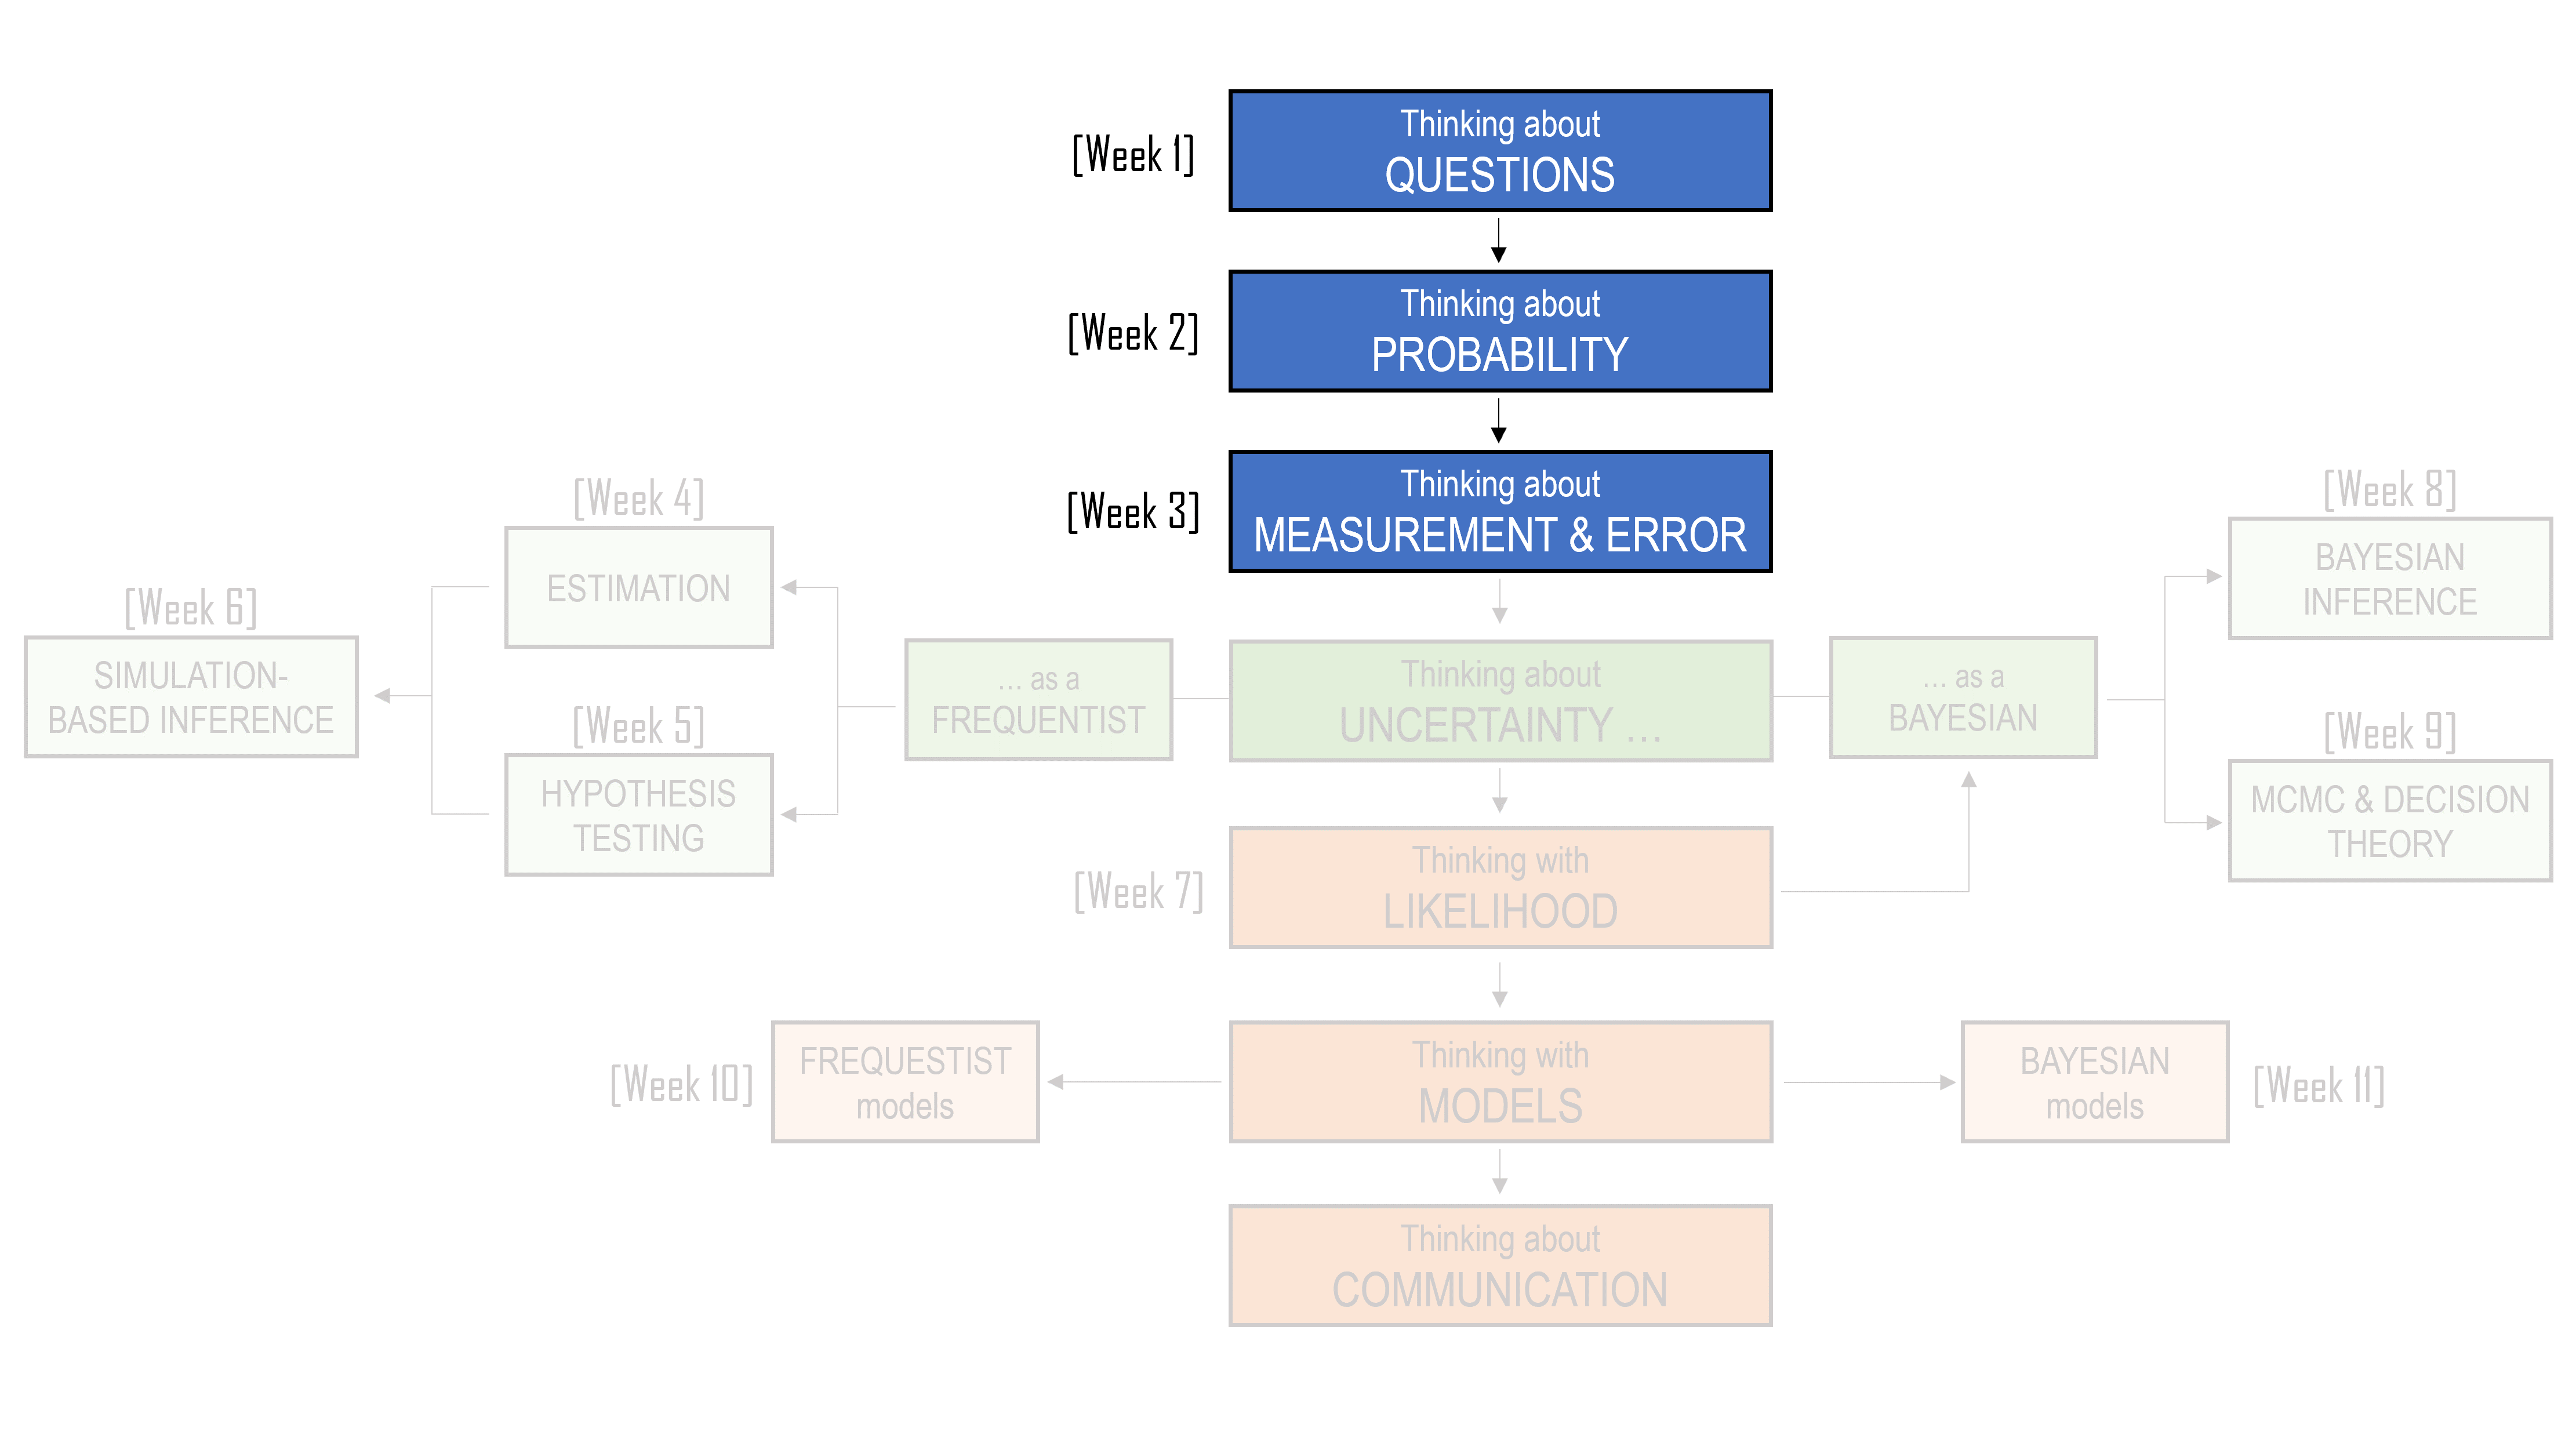
\includegraphics[width=14.81in,height=\textheight,keepaspectratio]{images/chapter3/outline.png}

\section{When one number feels more precise than it
is}\label{when-one-number-feels-more-precise-than-it-is}

Imagine standing in a bottle shop, looking at two bottles of wine:

\pandocbounded{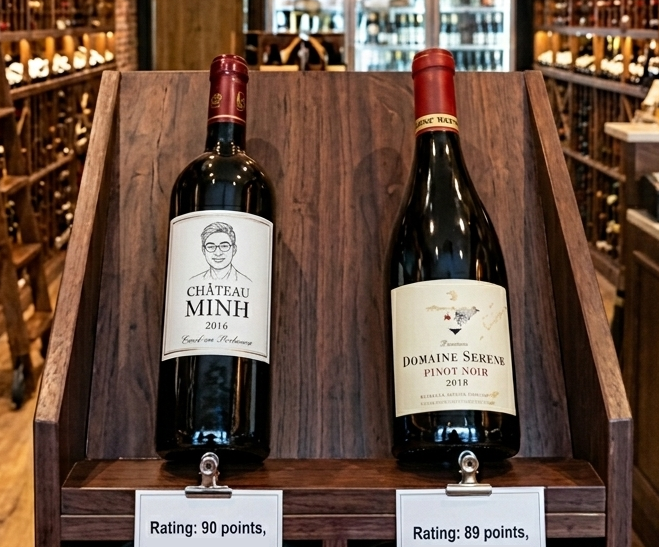
\includegraphics[keepaspectratio]{images/chapter3/Wine.png}}

One point separates them. One point may be enough to change what a
customer buys, what a shop charges, and what a winemaker can proudly
print on the next vintage. But what does that one point really mean?

If the same critic tasted the same wine tomorrow, would it still receive
a 90? If another critic tasted it, would they agree? If the bottle were
tasted after lunch rather than before lunch, in a warm room rather than
a cool one, after a different sequence of wines, or without knowing the
label, would the score be the same? The number looks precise. But the
process that produced the number is not perfectly precise. This is the
problem of measurement.

In statistics, we often work with numbers as if they are straightforward
facts. A wine receives 90 points. A student receives 73 on an exam. A
political party receives 52\% support in a poll. A car is measured
travelling at 64 kilometres per hour. A country's unemployment rate is
reported as 4.1\%. A candidate receives 12,431 votes. These numbers can
be useful. They may even be the best information we have. But they are
not the same as the thing we are trying to understand. They are
measurements of that thing.

\begin{itemize}
\tightlist
\item
  A wine score is not wine quality itself
\item
  An exam mark is not understanding itself
\item
  A poll result is not public opinion itself
\item
  A speed reading is not speed itself
\item
  A vote count is not democracy itself
\end{itemize}

Each number is produced by a process. And every process can introduce
uncertainty. To see this more clearly, consider the wine rating again.
Suppose we ask five critics to taste the same bottle independently.
Their ratings might look like this:

\begin{table}
\fontsize{12.0pt}{14.0pt}\selectfont
\begin{tabular*}{\linewidth}{@{\extracolsep{\fill}}lr}
\toprule
Critic & Rating \\ 
\midrule\addlinespace[2.5pt]
Critic 1 & 88 \\ 
Critic 2 & 90 \\ 
Critic 3 & 91 \\ 
Critic 4 & 89 \\ 
Critic 5 & 92 \\ 
\bottomrule
\end{tabular*}
\end{table}

None of these ratings needs to be a mistake. The critics may all be
experienced. They may all be tasting carefully. They may all be trying
to be fair. Yet they do not produce exactly the same number.

The variation may come from many sources.

\begin{itemize}
\tightlist
\item
  One critic may be more sensitive to acidity.
\item
  Another may value aroma more highly.
\item
  One may have tasted the wine after a very different bottle, making
  this one seem lighter or heavier by comparison.
\item
  Another may simply be having a different kind of day. Even if the
  critic is the same person, the score may change from one tasting to
  the next.
\end{itemize}

This does not mean wine ratings are worthless. It means they should be
interpreted as measurements rather than truths. A useful way to think
about this is:

\[
\text{Observed value} = \text{True value} + \text{Error}
\]

At this stage, we should not treat this as a perfect formula. It is more
like a statistical habit of mind. It reminds us that the number we
observe is not always the exact value we care about. For the wine
example, we might imagine:

\[
\text{Observed wine rating} = \text{Wine quality} + \text{Rating error}
\]

The difficult part is that we usually do not get to see the true value
directly. We see only the observed value. That is why measurement
matters. The same issue appears in many everyday situations.

\begin{table}
\fontsize{12.0pt}{14.0pt}\selectfont
\begin{tabular*}{\linewidth}{@{\extracolsep{\fill}}lll}
\toprule
Situation & What we want to know & What we observe \\ 
\midrule\addlinespace[2.5pt]
Wine tasting & Quality of the wine & A critic's score \\ 
Essay grading & Student understanding & A mark or grade \\ 
Speed detection & Actual speed of the car & A radar reading \\ 
Political polling & Public opinion & A survey estimate \\ 
Election counting & Voters' choices & A recorded vote count \\ 
Medical testing & Health status & A test result \\ 
\bottomrule
\end{tabular*}
\end{table}

In each case, there is a gap between the thing we want to know and the
number we record. Sometimes the gap is small. Sometimes it is large.
Sometimes it is mostly random. Sometimes it is systematic. Sometimes it
comes from the measuring instrument. Sometimes it comes from the person
doing the measuring. Sometimes it comes from the way the question was
asked, the way categories were defined, or the way observations were
collected. This is why a number can be both informative and uncertain.

Consider exam marks. If a student receives 73, we often behave as though
73 is an exact measurement of performance. But what if a different
marker would have given the same answer 75? What if the same student,
with the same level of understanding, would have scored 69 on a slightly
different version of the exam? What if one question happened to focus on
a topic the student revised the night before, while another equally
valid question would have exposed a weakness? Again, this does not mean
marks are meaningless. It means they are measurements. They contain
information, but they also contain error.

The same applies to polling. Suppose a poll reports that 52\% of
respondents support a particular policy. It is tempting to say:

\begin{quote}
52\% of people support the policy.
\end{quote}

But the poll did not ask everyone. It asked a sample of people. A
different sample might have produced 50\%, or 53\%, or 48\%. The
reported number is an estimate produced by a measurement process. A more
careful statement would be:

\begin{quote}
In this poll, using this sampling method, 52\% of respondents supported
the policy.
\end{quote}

That version is less dramatic, but more honest.

This chapter is about learning to think in that more careful way. We
will not stop using numbers. Statistics depends on numbers. But we will
stop pretending that numbers speak for themselves.

Instead, whenever we see a number, we will ask:

\begin{quote}
How was this number produced?
\end{quote}

\section{Two kinds of error}\label{two-kinds-of-error}

Once we accept that measurement is not the same as truth, the next
question is:

\begin{quote}
In what way can a measurement be wrong?
\end{quote}

Not all errors are the same. Some errors bounce around unpredictably.
Others lean consistently in one direction. This distinction is one of
the most important ideas in statistics.

Imagine a bathroom scale. You step on it five times in a row and it
gives these readings:

\begin{table}
\fontsize{12.0pt}{14.0pt}\selectfont
\begin{tabular*}{\linewidth}{@{\extracolsep{\fill}}lr}
\toprule
Attempt & Scale reading (kg) \\ 
\midrule\addlinespace[2.5pt]
Attempt 1 & 70.1 \\ 
Attempt 2 & 69.8 \\ 
Attempt 3 & 70.3 \\ 
Attempt 4 & 69.9 \\ 
Attempt 5 & 70.0 \\ 
\bottomrule
\end{tabular*}
\end{table}

The readings are not identical, but they are close. One reading is
slightly high, another slightly low. The differences might be due to how
you stood on the scale, tiny changes in the floor, or small
imperfections in the instrument. This is an example of \textbf{random
error}.

Random error is the kind of error that varies from measurement to
measurement. Sometimes it pushes the observed value a little too high.
Sometimes it pushes it a little too low. It does not follow an obvious
direction in a single observation, but over repeated measurements we may
begin to see its pattern.

Now imagine a different scale. This scale is faulty. Every time you step
on it, it adds \textasciitilde2 kilograms. If your true weight is 70
kilograms, the scale might show:

\begin{table}
\fontsize{12.0pt}{14.0pt}\selectfont
\begin{tabular*}{\linewidth}{@{\extracolsep{\fill}}lrr}
\toprule
Attempt & True weight (kg) & Scale reading (kg) \\ 
\midrule\addlinespace[2.5pt]
Attempt 1 & 70 & 72.1 \\ 
Attempt 2 & 70 & 71.8 \\ 
Attempt 3 & 70 & 72.3 \\ 
Attempt 4 & 70 & 71.9 \\ 
Attempt 5 & 70 & 72.0 \\ 
\bottomrule
\end{tabular*}
\end{table}

The readings still vary a little, but they are all centred around the
wrong value. The scale is not merely noisy. It is biased upward. This is
an example of \textbf{systematic error}.

Systematic error occurs when a measurement process tends to push the
observed value in a particular direction.

\begin{itemize}
\tightlist
\item
  A faulty scale may always read too high.
\item
  A poorly worded survey question may consistently encourage one kind of
  answer.
\item
  A wine critic may consistently favour expensive labels.
\item
  A speed camera may be miscalibrated.
\item
  A test may consistently advantage students who are familiar with a
  particular cultural context.
\end{itemize}

The difference between random error and systematic error can be
summarised like this:

\begin{table}
\fontsize{12.0pt}{14.0pt}\selectfont
\begin{tabular*}{\linewidth}{@{\extracolsep{\fill}}lll}
\toprule
Type of error & Description & Example \\ 
\midrule\addlinespace[2.5pt]
Random error & The measurement varies unpredictably from one observation to the next. & A wine receives 88, 90, and 91 from different critics. \\ 
Systematic error & The measurement is consistently pushed in one direction. & A scale always reads 2 kg too high. \\ 
\bottomrule
\end{tabular*}
\end{table}

Random error can often be reduced by taking repeated measurements. If
five wine critics independently rate the same bottle, their average
rating may be more stable than any one critic's score. If we weigh an
object several times, the average reading may be more reliable than a
single reading. If we survey more people, the random variation caused by
sampling can become smaller.

But repeated measurement does not automatically fix systematic error. If
a scale is always 2 kilograms too high, weighing yourself one hundred
times will not solve the problem. The average of the one hundred
readings will still be about 2 kilograms too high. If a poll
systematically misses a group of voters, increasing the sample size may
give us a very precise estimate of the wrong population. If a wine
critic is influenced by the label, asking them to taste the wine
repeatedly while still seeing the label may simply reproduce the same
bias.

Consider political polling. Suppose a survey is conducted before an
election. There are at least two different ways the result might be
wrong. First, by chance, the sample might include slightly too many
supporters of one party. If another random sample were taken, the result
might be slightly different. This is random error. Second, the survey
might systematically miss young renters, people who work irregular
hours, or people who do not answer unknown phone numbers. If those
people vote differently from the people who are reached, the poll may be
biased. This is systematic error. The two problems require different
responses. To reduce random sampling error, we might increase the sample
size. To reduce systematic error, we need to improve the measurement
process: who is sampled, how they are contacted, how responses are
weighted, and how questions are asked.

The same idea applies to grading. Suppose two markers grade the same
essay. One gives it 72 and another gives it 76. That difference may
reflect random variation in judgement. A clear rubric, double marking,
or averaging across markers may help. But suppose an assessment
systematically rewards students who already know a particular social,
cultural, or professional context. In that case, the assessment may be
biased. Marking more essays will not fix the problem. The measurement
process itself needs to be examined.

The wine example shows both forms of error. A critic might give the same
wine slightly different scores on different days. That is random error.
But if the critic consistently gives higher scores to wines with
prestigious labels, that is systematic error. If the tasting is not
blind, the score may reflect both the wine and the critic's
expectations. This is why blind tasting is so valuable. It is not
designed to remove all variation. Critics may still disagree. But it can
reduce one particular source of systematic error: the influence of
knowing the label, price, region, or reputation of the wine.

We can now return to the simple measurement equation from the previous
section:

\[
\text{Observed value} = \text{True value} + \text{Error}
\]

We can make it more informative by separating error into two parts:

\[
\text{Observed value} = \text{True value} + \text{Systematic error} + \text{Random error}
\]

This formula is still a simplification. In real settings, the ``true
value'' may be difficult to define, and the two kinds of error may be
tangled together. But the formula gives us a useful way to think. For
example:

\[
\text{Observed wine score} =
\text{Wine quality}
+
\text{Critic bias}
+
\text{Tasting variation}
\]

When we see a number, we should ask:

\begin{itemize}
\tightlist
\item
  Could this number be a little different if the measurement were
  repeated?
\item
  Is the measurement process likely to push the number consistently
  upward or downward?
\item
  Would more observations help?
\item
  Or is the problem built into the way the measurement is being made?
\end{itemize}

These questions will return throughout the chapter. They are also the
reason probability becomes so important for statistics. If random error
is part of measurement, then we need a way to understand how much random
variation to expect.

That is where the next example (Joseph Jagger) takes us.

\begin{tcolorbox}[enhanced jigsaw, arc=.35mm, bottomrule=.15mm, bottomtitle=1mm, breakable, colback=white, colbacktitle=quarto-callout-note-color!10!white, colframe=quarto-callout-note-color-frame, coltitle=black, left=2mm, leftrule=.75mm, opacityback=0, opacitybacktitle=0.6, rightrule=.15mm, title=\textcolor{quarto-callout-note-color}{\faInfo}\hspace{0.5em}{Case Study: Joseph Jagger}, titlerule=0mm, toprule=.15mm, toptitle=1mm]

Joseph Jagger (1830 - 1892) not a magician, psychic, or gambler in the
usual romantic sense. He was an engineer and mechanic from Yorkshire,
and that background mattered. He understood machines. He knew that real
machines are not perfect mathematical objects. They wear down. They
wobble. Their surfaces become uneven. Their parts are made, assembled,
repaired, and used by human beings.

Roulette, however, depends on the idea that the wheel behaves as though
it were perfect. A European roulette wheel has 37 numbered compartments:
1 through 36, plus 0. When the wheel is spun, a small ball eventually
lands in one of these compartments. If the wheel is fair, each number
should have the same chance of appearing:

\[
P(\text{any particular number}) = \frac{1}{37}
\]

The casino pays less than true fairness would require. If you bet on a
single number and win, you are paid 35 to 1, even though there are 37
possible outcomes. That difference is the house edge. In the long run,
if the wheel is fair, the casino wins. But Jagger asked a different
question:

\begin{quote}
What if the wheel is not fair?
\end{quote}

This was a measurement question. Jagger was not trying to predict the
next spin by luck or intuition. He was trying to measure the behaviour
of the wheel. In 1873, he travelled to Monte Carlo with his savings and
hired six assistants, one for each of the casino's roulette wheels.
Their task was simple but tedious: watch the wheels and record the
numbers that came up. Each day, while the casino was open, the
assistants collected observations. Each night, Jagger analysed the
counts.

For six days, he looked for a pattern. On five of the wheels, he found
nothing useful. The numbers varied, of course, but not in a way that
gave him confidence. On the sixth wheel, however, something stood out.
Nine numbers appeared more often than expected:

\[
7,\ 8,\ 9,\ 17,\ 18,\ 19,\ 22,\ 28,\ 29
\]

Jagger had found what every statistician hopes to find when analysing
noisy data: a possible signal. The next day, he went to the casino and
began betting heavily on those nine numbers. By the end of the day, he
was up \$70,000. This is the dramatic part of the story, but the
statistical part is even more important. Jagger won because he treated
the roulette wheel as a physical measurement system. He did not assume
that the official probabilities were correct. He collected data and
compared what the wheel actually did with what a fair wheel should have
done.

We can summarise his reasoning like this:

\begin{table}
\fontsize{12.0pt}{14.0pt}\selectfont
\begin{tabular*}{\linewidth}{@{\extracolsep{\fill}}ll}
\toprule
Step & Jagger's investigation \\ 
\midrule\addlinespace[2.5pt]
1. Statistical model & A fair roulette wheel should give each number probability 1/37 \\ 
2. Measurement & Assistants recorded the numbers produced by each wheel \\ 
3. Comparison & Jagger compared observed counts with what fairness would suggest \\ 
4. Interpretation & One wheel seemed to favour certain number. \\ 
5. Action & Jagger bet on the numbers that appeared too often \\ 
\bottomrule
\end{tabular*}
\end{table}

The casino quickly realised something was wrong. Other players noticed
Jagger winning and began following his bets. Inspectors watched him
closely, looking for cheating or a hidden trick. But Jagger was not
cheating. He was exploiting measurement error in the wheel.

Over the next few days, his winnings grew. By the fourth day of betting,
he had accumulated around \$300,000. The casino needed to stop him. They
did something clever. They switched the wheel. At first, Jagger began to
lose. This is an important detail. He did not lose every spin, just as
he had not won every spin before. Gambling, even with an advantage,
still contains randomness. But now the balance had changed. Previously,
he had been winning more often than losing. After the switch, he was
losing more often than winning. This is what makes signal and noise
difficult. The change did not announce itself instantly. It appeared
through the accumulation of results.

Jagger eventually noticed something small but crucial. During his
winning days, he had seen a tiny scratch on the wheel. Now the scratch
was gone. The most likely explanation was not that the scratch had been
repaired. It was that the casino had moved the wheel. So Jagger looked
around. Another wheel had the scratch. He moved to that wheel and began
winning again.

This moment is worth pausing over. Jagger's success depended on
recognising that his data were attached to a particular physical object.
The favourable numbers were not magical numbers. They were not lucky
numbers. They belonged to one imperfect wheel. Once the wheel changed,
the pattern changed. A pattern may exist only under a particular
measurement process. Change the process, and the pattern may disappear.

Eventually, the casino worked out more of what was happening. They began
moving the frets, the dividers between the numbered compartments, so
that the wheel's imbalance would favour different numbers each day. Once
the favoured numbers changed, Jagger's advantage disappeared. He began
losing again and finally stopped. Even so, he left Monte Carlo with
about \$325,000, a huge sum at the time.

Jagger had beaten the casino, but not by defeating randomness. He won by
discovering that the randomness was not quite random. If a roulette
wheel is perfectly fair, uneven results will still occur. Some numbers
will appear more often than others over a short period. A fair wheel
does not politely arrange itself so that every number appears exactly
the same number of times. Randomness produces clusters, streaks, gaps,
and surprises. So when Jagger observed that some numbers appeared more
often than others, there were two possible explanations:

\begin{table}
\fontsize{12.0pt}{14.0pt}\selectfont
\begin{tabular*}{\linewidth}{@{\extracolsep{\fill}}lll}
\toprule
Possible explanation & Meaning & What we would expect over time \\ 
\midrule\addlinespace[2.5pt]
Random variation & The wheel is fair, but chance has produced uneven counts. & The apparent pattern may disappear with more spins. \\ 
Systematic bias & The wheel is physically imperfect, so some numbers really are more likely. & The pattern may persist as long as the same wheel is used. \\ 
\bottomrule
\end{tabular*}
\end{table}

Jagger's problem was to decide whether the observed pattern was large
and persistent enough to act on. That is the problem of signal and
noise.

\begin{itemize}
\tightlist
\item
  A signal is a real pattern that tells us something about the process
  being measured. In Jagger's case, the signal was the wheel's physical
  bias.
\item
  Noise is random variation that looks meaningful but does not reflect a
  real underlying pattern. A fair wheel might make one number appear
  unusually often for a while, but that does not mean the number is
  truly favoured.
\end{itemize}

\begin{table}
\fontsize{12.0pt}{14.0pt}\selectfont
\begin{tabular*}{\linewidth}{@{\extracolsep{\fill}}lll}
\toprule
Term & General meaning & Jagger example \\ 
\midrule\addlinespace[2.5pt]
Signal & A real pattern in the process being measured. & A physical imperfection makes some roulette numbers more likely. \\ 
Noise & Random variation that may look like a pattern. & A fair wheel happens to produce uneven counts over a short run. \\ 
\bottomrule
\end{tabular*}
\end{table}

This is why Jagger needed many observations. One spin tells us almost
nothing. Ten spins tell us very little. Even after many spins, there is
still a chance that the apparent pattern is just luck. But the more data
Jagger collected, the more clearly he could compare the wheel's observed
behaviour with the behaviour expected from a fair wheel.

The lesson is not that every apparent pattern should be trusted. It is
almost the opposite. Many patterns are illusions. If we stare at random
data for long enough, some parts of it will look meaningful.

\begin{itemize}
\tightlist
\item
  A roulette number may appear several times in a short sequence.
\item
  A student may receive a surprisingly high mark on one test.
\item
  A player may score in several consecutive games.
\item
  A poll may move by two percentage points.
\item
  A wine may receive one unusually high rating.
\end{itemize}

None of these automatically proves that something real has changed.

But Jagger's story also shows that not every pattern is an illusion.
Sometimes the wheel really is biased. Sometimes the measurement process
really is distorted. Sometimes the observed results are trying to tell
us something. The statistical challenge is to decide which situation we
are in.

Jagger's investigation began with the assumption of fairness:

\[
P(0) = P(1) = P(2) = \cdots = P(36) = \frac{1}{37}
\]

His data suggested that this assumption might not hold for one
particular wheel. By comparing observed results with expected results,
he reasoned backwards from data to process.

In probability, we often begin with a model and ask:

\begin{quote}
If the wheel is fair, what results could it produce?
\end{quote}

In statistics, we often begin with results and ask:

\begin{quote}
Given what we observed, does the wheel look fair?
\end{quote}

Jagger's story sits exactly at that turning point. It shows how data can
be used to investigate an unseen process. It also shows why we must be
careful. Random variation can create false patterns, but systematic bias
can create real ones. Jagger won because he found a real bias hiding
inside what was supposed to be a random system. The next question is how
this becomes possible at all. Why does collecting more observations
help? Why are short runs so unreliable, while long runs can reveal
structure?

That takes us to Bernoulli and the law of large numbers.

\end{tcolorbox}

\section{Bernoulli and the law of large
numbers}\label{bernoulli-and-the-law-of-large-numbers}

Jacob Bernoulli was born in Basel, Switzerland, in 1654, into a family
that would become one of the most remarkable mathematical families in
European history. Several Bernoullis became famous mathematicians, but
Jacob was one of the first to see that probability might become
something more than a set of clever rules for gambling.

\begin{figure}[H]

{\centering 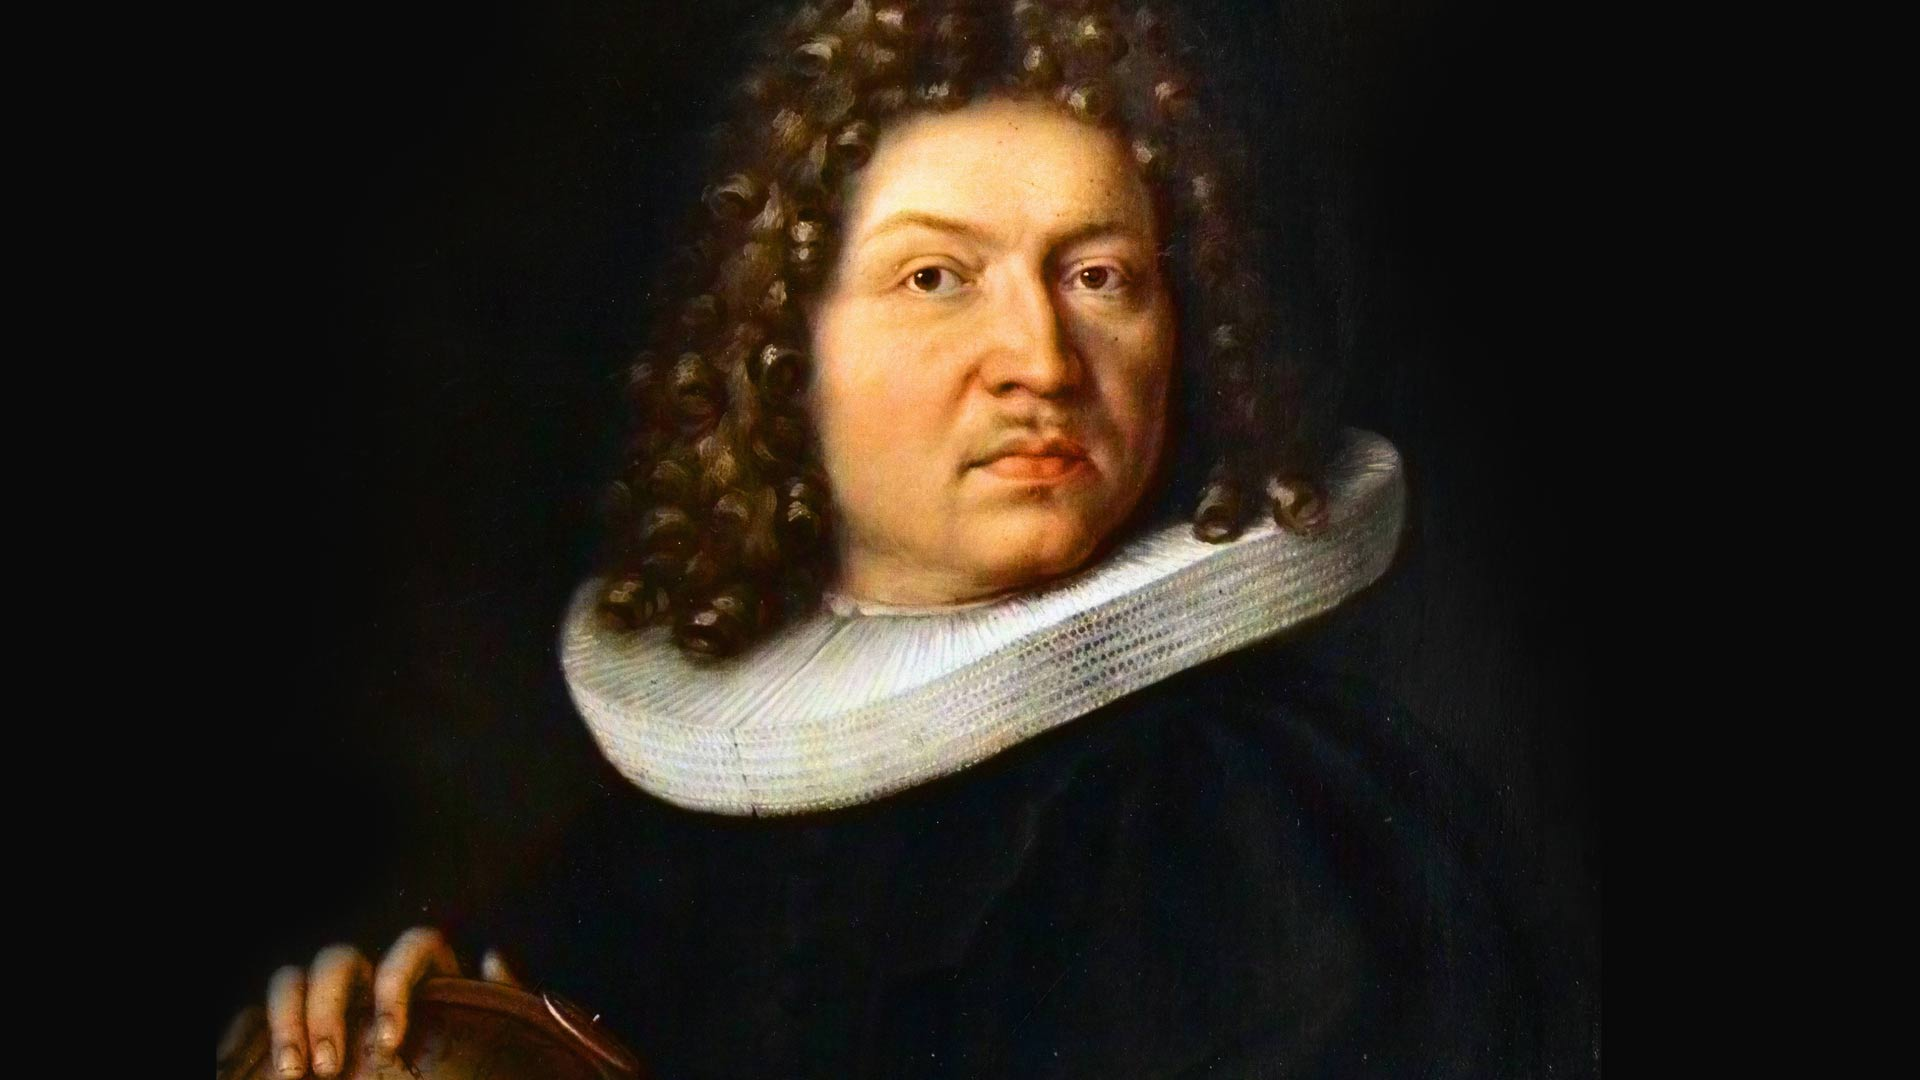
\includegraphics[width=6.4in,height=\textheight,keepaspectratio]{images/chapter3/Bernoulli.jpg}

}

\caption{Image Source: https://www1.wdr.de/stichtag/stichtag-392.html}

\end{figure}%

In the world Bernoulli inherited, probability was closely tied to games
of chance. Dice, cards, lotteries, and wagers were the natural places to
think mathematically about uncertainty. This made sense. In many games,
the possible outcomes are clearly defined. A die has six faces. A deck
has a fixed number of cards. A lottery has a known number of tickets. If
we know the structure of the game, we can often calculate the
probability before anything happens.

For example, if a fair die is rolled, the probability of rolling a six
is:

\[
P(\text{six}) = \frac{1}{6}
\]

If a fair coin is tossed, the probability of heads is:

\[
P(\text{heads}) = \frac{1}{2}
\]

These probabilities come from symmetry. We do not need to toss the coin
10,000 times to know that a fair coin has two equally possible sides. We
do not need to roll the die forever to know that a fair six-sided die
has six equally possible faces. For games of chance, this approach is
powerful.

But Bernoulli saw a problem. What about events where the possible
outcomes are not arranged so neatly?

\begin{itemize}
\tightlist
\item
  What is the probability that a person of a certain age will die within
  the next year?
\item
  What is the probability that a medical treatment will work?
\item
  What is the probability that a witness is telling the truth?
\item
  What is the probability that a political candidate will win an
  election?
\item
  What is the probability that a machine is faulty?
\end{itemize}

In these cases, there is no obvious die to inspect. There may be no
clean sample space. We cannot simply count equally likely cases and
divide. So where do the probabilities come from? Bernoulli's answer was
that, in many cases, probabilities must be learned through observation.

This is the key link back to Jagger. Joseph Jagger came after Bernoulli,
but his method illustrates Bernoulli's idea beautifully. Jagger did not
know the true probabilities of the roulette wheel in advance.
Officially, each number on a European roulette wheel should have
probability:

\[
\frac{1}{37}
\]

But Jagger suspected that the actual wheel might not behave like the
official mathematical wheel. So he observed it. He counted outcomes. He
looked for stable patterns in repeated spins. In other words, he treated
probability not only as something calculated from an ideal model, but as
something that could be discerned through data. That shift is enormous.
It moves probability from the gambling table into the world.

Bernoulli wanted to understand how repeated observations could teach us
about an unknown probability. If we observe enough cases, can the
pattern in the data reveal the underlying chance process?

Before stating his famous result, it is useful to pause on a
mathematical idea that sits quietly behind it: the idea of approaching a
limit. A limit is a value that a sequence gets closer and closer to,
even if the early terms jump around or even if the value is never
reached exactly at any particular step. One of the oldest ways to feel
this idea is through Zeno's paradox.

\begin{tcolorbox}[enhanced jigsaw, arc=.35mm, bottomrule=.15mm, bottomtitle=1mm, breakable, colback=white, colbacktitle=quarto-callout-note-color!10!white, colframe=quarto-callout-note-color-frame, coltitle=black, left=2mm, leftrule=.75mm, opacityback=0, opacitybacktitle=0.6, rightrule=.15mm, title=\textcolor{quarto-callout-note-color}{\faInfo}\hspace{0.5em}{Zeno's Paradox}, titlerule=0mm, toprule=.15mm, toptitle=1mm]

Zeno of Elea (c.~490--430 BC) was a pre-Socratic Greek philosopher from
the city of Elea. He is famous for creating thought experiments, or
paradoxes, that challenge our understanding of space, time, and motion.

One of his paradoxes goes something like this:

\begin{quote}
Suppose Atalanta wishes to walk to the end of a path. Before she can get
there, she must get halfway there. Before she can get halfway there, she
must get a quarter of the way there. Before traveling a quarter, she
must travel one-eighth; before an eighth, one-sixteenth; and so on.
\end{quote}

\pandocbounded{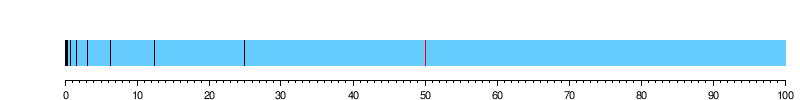
\includegraphics[keepaspectratio]{images/chapter3/zeno.png}}

There are infinitely many pieces in this sequence. That seems troubling.
If Atalanta must complete infinitely many pieces of the journey, how can
she ever arrive?

\[
\frac{1}{2},\ \frac{1}{4},\ \frac{1}{8},\ \frac{1}{16},\ \ldots
\]

At first, Zeno's reasoning feels persuasive. Every time Atalanta
completes one part of the journey, another smaller part remains. The
process never seems to end. But the important detail is that the pieces
are not all the same size. They shrink very quickly.

This is exactly the sort of situation where the ideas of sequence,
series, and limit become useful. Rather than trying to add infinitely
many terms at once, let us look at the journey one stage at a time.

After the first interval, Atalanta has travelled:

\[
\frac{1}{2} \text{ of a meter}
\]

After the second interval, she has travelled:

\[
\frac{1}{2} + \frac{1}{4} = \frac{3}{4} \text{ of a meter}
\]

After the third interval, she has travelled:

\[
\frac{1}{2} + \frac{1}{4} + \frac{1}{8} = \frac{7}{8} \text{ of a meter}
\]

After the fourth interval, she has travelled:

\[
\frac{1}{2} + \frac{1}{4} + \frac{1}{8} + \frac{1}{16} = \frac{15}{16} \text{ of a meter}
\]

These totals form a new sequence:

\[
\frac{1}{2},\ \frac{3}{4},\ \frac{7}{8},\ \frac{15}{16},\ \ldots
\]

There is a clear pattern. The denominators are powers of 2, and the
numerators are always one less than the denominator. So after 10
intervals, Atalanta would have traveled:

\[
\frac{1023}{1024} \text{ of a meter}
\]

After 20 intervals, she would have travelled:

\[
\frac{1{,}048{,}575}{1{,}048{,}576} \text{ of a meter}
\]

Each additional interval takes Atalanta a little farther. Zeno was right
about that. The total keeps increasing. But the total is not racing off
toward infinity. Instead, it is getting closer and closer to 1 meter.

In mathematical language, we say that 1 is the limit of the sequence of
partial sums:

\[
\lim_{n \to \infty}
\sum_{k = 1}^{n} \frac{1}{2^k}
= 1
\]

For our purposes, the deeper lesson is not about walking across a room.
It is about what it means for a sequence to settle toward a value. A
process can keep going, step after step, while the accumulated result
approaches a fixed limit.

\end{tcolorbox}

Just as Zeno's partial distances get closer and closer to 1 meter,
Bernoulli showed that long-run relative frequencies can get closer and
closer to the probabilities that generate them. Zeno helps us understand
the idea of approaching a limit; Bernoulli applies a similar way of
thinking to repeated observations under uncertainty.

Bernoulli worked on this result for nearly 20 years and regarded it as
one of his greatest achievements. He called it his ``golden theorem.''
Today, it is usually known as the law of large numbers. The theorem has
many real-world applications, but its central message is simple: a small
number of observations may be misleading, while a large number of
repeated observations can begin to reveal the underlying probability. We
will start with a simple example of the kind Bernoulli himself used,
which I have modified slightly for the modern reader:

\emph{Suppose a box contains 300 white balls and 200 black balls. In
other words, 60\% of the balls are white and 40\% are black. Now imagine
drawing one ball at random, recording its colour, placing it back in the
box, mixing the balls, and drawing again. Because the ball is replaced
each time, the probability of drawing a white ball remains the same on
every draw:}

\(P(white)=300/500=0.60\)

Bernoulli's question was not simply whether white balls are more likely
than black balls. In this example, we already know that they are. His
deeper question was about repeated observation:

\begin{quote}
If the true probability of drawing a white ball is 60\%, how close
should the observed proportion of white balls be to 60\% after many
draws, and how confident can we be that it will be close?
\end{quote}

A small number of draws may easily give a proportion quite far from
60\%. But as the number of draws increases, Bernoulli showed that the
observed proportion should become increasingly likely to lie near the
true probability.

After 10 draws, we might observe 7 white balls:

\[
\hat{p} = \frac{7}{10} = 0.7.
\]

After 100 draws, we might observe 63 white balls:

\[
\hat{p} = \frac{63}{100} = 0.63.
\]

After 1000 draws, we might observe 604 white balls:

\[
\hat{p} = \frac{604}{1000} = 0.604.
\]

The observed proportion is not exactly 0.6 at every stage. It can
wander. But with more observations, it tends to become more stable.

\begin{table}
\fontsize{12.0pt}{14.0pt}\selectfont
\begin{tabular*}{\linewidth}{@{\extracolsep{\fill}}rrr}
\toprule
Number of draws & Black balls observed & Observed proportion \\ 
\midrule\addlinespace[2.5pt]
10 & 7 & 0.700 \\ 
100 & 63 & 0.630 \\ 
1000 & 604 & 0.604 \\ 
10000 & 5991 & 0.599 \\ 
\bottomrule
\end{tabular*}
\end{table}

In notation, we might write:

\[
\hat{p}_n \to p
\]

where \(\hat{p}_n\) is the observed proportion after \(n\) observations,
and \(p\) is the true underlying probability.

This small piece of notation contains a large idea. The observed
proportion is not guaranteed to equal the true probability. It is not
guaranteed to move smoothly. It may jump around, especially early on.
But with enough observations, it tends to settle.

A simulation makes this easier to see:

\pandocbounded{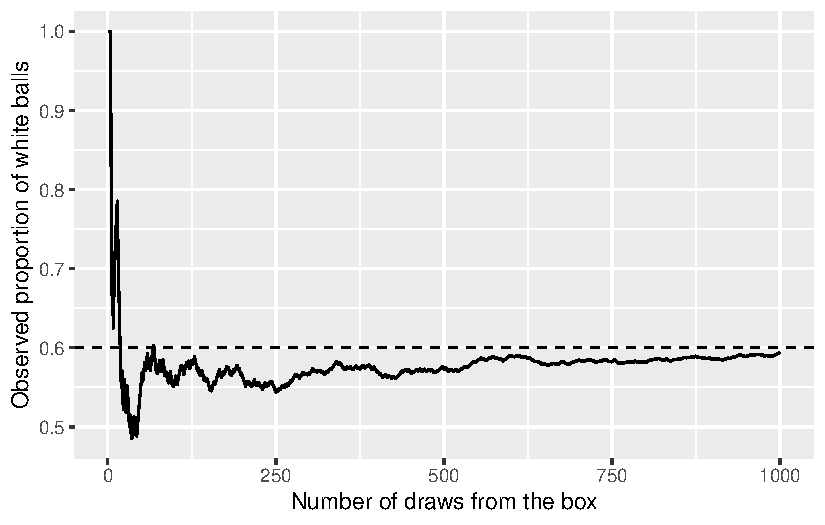
\includegraphics[keepaspectratio]{3_MeasurementError_files/figure-pdf/unnamed-chunk-13-1.pdf}}

In the early draws, the proportion may move sharply. One extra white
ball can change the observed proportion dramatically. Later, each new
draw has less influence on the accumulated proportion. The line may
still wander, but it usually wanders less. This is why repeated
observation is powerful.

However, we need to be careful. The law of large numbers does not say
that more data automatically give us the truth. It helps with random
variation, not necessarily systematic bias. If a box is shaken properly
and the draws are made fairly, repeated draws can help us learn its
composition. But if the balls are not mixed, or if one colour is easier
to draw, or if someone records the colours incorrectly, then more
observations may simply give us a more precise version of the wrong
answer.

The same warning applies everywhere.

\begin{itemize}
\tightlist
\item
  A large poll can still be biased if it misses part of the population.
\item
  A large set of wine ratings can still be biased if all critics are
  influenced by the label.
\item
  A large number of exam marks can still mislead if the assessment does
  not measure the kind of understanding we care about.
\item
  A roulette wheel can only be studied properly if we know which
  physical wheel produced the observations.
\end{itemize}

This is the lesson that connects Bernoulli back to measurement. Repeated
observations can reduce random error. They can help us see stable
patterns. They can allow us to estimate probabilities that cannot be
calculated in advance. But they do not remove the need to ask how the
data were produced.

\section{The danger of small numbers}\label{the-danger-of-small-numbers}

Consider a simple coin example. Suppose you watch someone flip a coin
four times, and the result is:

\[
H,\ H,\ H,\ H
\]

Four heads in a row feels suspicious. It is natural to wonder whether
the coin is biased, or whether the person flipping it is doing something
unusual. But before we jump to that conclusion, we should ask: how
surprising is this result if the coin is actually fair?

For a fair coin, the probability of heads on each flip is:

\[
P(H) = \frac{1}{2}
\]

So the probability of four heads in a row is:

\[
P(HHHH) =
\frac{1}{2}
\times
\frac{1}{2}
\times
\frac{1}{2}
\times
\frac{1}{2}
= \frac{1}{16}
= 0.0625
\]

So four heads in a row is unusual, but not astonishing (6.25\%). If many
people flipped coins four times, we would expect some of them to get
four heads. Seeing four heads should make us curious, but it is not
enough on its own to prove that the coin is biased.

Now suppose the same person flips the coin ten times, and the result is:

\[
H,\ H,\ H,\ H,\ H,\ H,\ H,\ H,\ H,\ H
\]

This feels much more suspicious. Again, under the fair coin model:

\[
P(10 \text{ heads in a row})
= \left(\frac{1}{2}\right)^{10}
\frac{1}{1024}
\approx 0.00098
\]

Ten heads in a row does not logically prove that the coin is biased.
Rare events can happen. But it gives us much stronger reason to question
the fairness of the coin than four heads in a row. The same kind of
result can mean different things depending on how much evidence we have.
Four heads in a row may be a coincidence. Ten heads in a row is harder
to dismiss.

But even then, we should be careful. The conclusion is not
automatically:

\begin{quote}
The coin is biased.
\end{quote}

A better conclusion is:

\begin{quote}
This result would be quite unlikely if the coin were fair, so the
fairness of the coin is worth questioning.
\end{quote}

Statistical thinking does not require us to ignore surprising patterns.
It asks us to compare those patterns with what chance alone might
reasonably produce. This is why small samples are dangerous. They often
look more informative than they really are.

Suppose a new café opens and receives two online reviews. Both are five
stars. It would be tempting to say:

\begin{quote}
This café is excellent.
\end{quote}

But two reviews are not enough to know. Perhaps the first two reviewers
were the owner's friends. Perhaps they happened to visit on a good day.
Perhaps they love that particular style of food. Perhaps the next ten
customers will be less impressed.

Now suppose the café has 200 reviews and an average rating of 4.8 stars.
That still does not prove the café is excellent, but it is stronger
evidence. The rating is based on many more experiences. A few unusually
enthusiastic customers have less power to dominate the average.

The same logic applies to wine ratings. If one critic gives a wine 95,
the rating may be informative, but it may also be unusual. Perhaps that
critic particularly likes the style. Perhaps the bottle tasted better
than usual. Perhaps the tasting conditions helped. If twenty independent
critics give the wine ratings between 93 and 96, the evidence is much
stronger.

Small numbers are also dangerous in sport. A basketball player who makes
4 shots out of 5 has an 80\% shooting rate for that small set of shots:

\[
\hat{p} = \frac{4}{5} = 0.8
\]

But we should be careful. Five shots do not tell us very much about the
player's long-run ability. A weaker shooter can make 4 out of 5 by
chance. A strong shooter can miss 4 out of 5 by chance. Short sequences
are noisy.

If the same player makes 400 shots out of 500, then the 80\% figure
becomes much more meaningful:

\[
\hat{p} = \frac{400}{500} = 0.8
\]

Again, the proportion is the same. The strength of the evidence is not.

\begin{table}
\fontsize{12.0pt}{14.0pt}\selectfont
\begin{tabular*}{\linewidth}{@{\extracolsep{\fill}}lrrrl}
\toprule
Situation & Shots made & Shots attempted & Shooting percentage & Careful interpretation \\ 
\midrule\addlinespace[2.5pt]
Small sample & 4 & 5 & 80\% & A short streak; interpret cautiously \\ 
Large sample & 400 & 500 & 80\% & Much stronger evidence of shooting ability \\ 
\bottomrule
\end{tabular*}
\end{table}

This is sometimes called the \textbf{law of small numbers}. The name is
a little playful, because it is not a true mathematical law like
Bernoulli's law of large numbers. It refers to a common mistake in human
thinking: the belief that a small sample should already look like the
larger population or process it came from.

We expect short sequences to behave too neatly. We expect 10 coin tosses
to look roughly like 50\% heads and 50\% tails. We expect a small poll
to resemble the electorate. We expect one exam to reveal a student's
true understanding. We expect a handful of reviews to reveal the quality
of a restaurant. We expect one week of sales to reveal whether a
business is succeeding.

But small samples do not have to behave. They can be lopsided. They can
be unrepresentative. They can produce extreme results. And because
extreme results attract attention, small samples can be especially
misleading. A useful way to remember this is:

\begin{quote}
The smaller the sample, the louder the noise.
\end{quote}

This does not mean we should ignore small samples. Sometimes small
samples are all we have. Early data can be useful. One poor quiz result
may suggest that a student needs help. One unusual medical result may
call for follow-up. A sudden change in sales may deserve attention.
Jagger himself began with observed imbalances before he knew whether
they were meaningful.

The point is not to dismiss small samples. The point is to treat them
with the right level of caution. A small sample can raise a question. It
should rarely settle the question.

Some quantities describe groups quite well, but fail when we apply them
too confidently to individuals. A life expectancy, for example, may
summarise many lives. But can it tell us how long one person will live?

That question takes us to Jeanne Calment.

\section{The problem of individual
prediction}\label{the-problem-of-individual-prediction}

Jeanne Calment was born in France in 1875. Her life stretched across an
almost unbelievable span of history. She was alive before the invention
of the modern automobile, before aeroplanes, before radio, before
television, before antibiotics, and before the First World War. As a
teenager, she even encountered Vincent van Gogh in her father's shop.

\begin{figure}[H]

{\centering 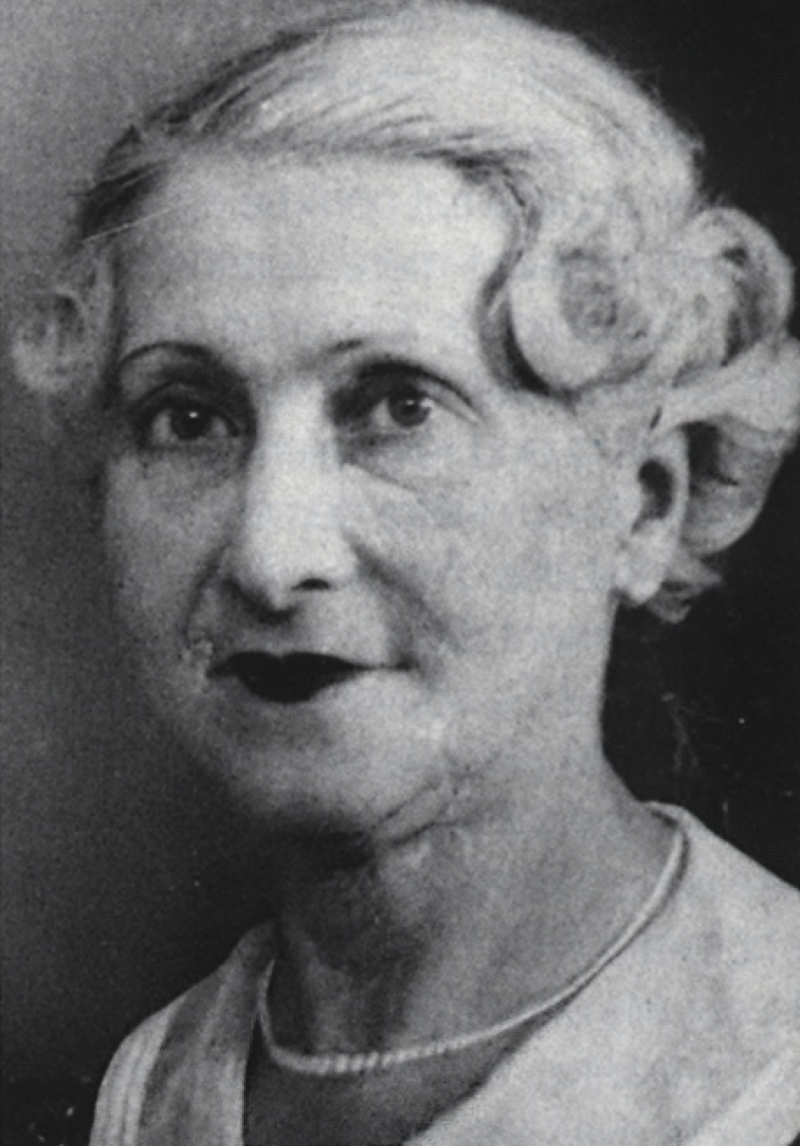
\includegraphics[width=0.5\linewidth,height=\textheight,keepaspectratio]{images/chapter3/jeanne.png}

}

\caption{Image Source: https://forgottennewsmakers.com/}

\end{figure}%

By the time Calment was 90 years old, she owned an apartment but needed
money to live on. So she made an arrangement with a 47-year-old lawyer.
The lawyer would pay her a small monthly amount for the rest of her
life. In exchange, when she died, he would inherit the apartment.

At first glance, this may have seemed like a sensible deal for the
lawyer. Calment was already 90. The lawyer was only 47. If she lived
only a few more years, he would eventually receive an apartment for far
less than its full value. But randomness had other plans. Calment turned
100. Then she turned 110. The lawyer kept paying. Then, in 1995, the
lawyer himself died. Calment was still alive. She eventually died in
1997 at the age of 122, becoming one of the longest-lived people ever
recorded.

The lawyer's mistake was not necessarily that he ignored statistics.
More likely, he misunderstood what the statistics could tell him. A
number such as life expectancy sounds as though it should answer a
simple question:

\begin{quote}
How long will this person live?
\end{quote}

But that is not quite what life expectancy does.

\begin{quote}
Life expectancy is a summary of a group. It tells us something about the
average pattern across many lives. It does not tell us the exact path of
one particular life.
\end{quote}

Suppose we say that the life expectancy of a certain population is 80
years. That does not mean every person dies at 80. Some people die in
infancy. Some die in early adulthood. Many die in old age. A small
number live far beyond 100. The average may be 80, but the individual
lives are scattered around that average.

In other words, the average is not a prophecy.

\begin{table}
\fontsize{12.0pt}{14.0pt}\selectfont
\begin{tabular*}{\linewidth}{@{\extracolsep{\fill}}lll}
\toprule
Question & Type of question & Careful interpretation \\ 
\midrule\addlinespace[2.5pt]
How long do people in this population live on average? & Population summary & Useful for describing a group, not a guarantee for each person. \\ 
How long does a person aged 90 usually live from now? & Conditional population summary & More relevant than life expectancy at birth, because the person has already reached 90. \\ 
How long will Jeanne Calment live? & Individual prediction & Highly uncertain, even with good population data. \\ 
\bottomrule
\end{tabular*}
\end{table}

There is another important detail. The relevant question for Calment was
not:

\begin{quote}
How long does the average person live from birth?
\end{quote}

The relevant question was:

\begin{quote}
Given that she has already reached 90, how much longer might she live?
\end{quote}

These are different questions.

A person who has already reached 90 has already survived all the risks
that might have ended life earlier. They did not die in childhood. They
did not die in a car accident at 25. They did not die of illness at 50.
They have already passed through many hazards. So their remaining life
expectancy is not calculated from birth. It is conditional on having
already reached 90.

This is an example of conditional thinking.

In probability language, we are not asking simply about the probability
of living to a certain age. We are asking about the probability of
living longer, given that a person has already lived to some age.

For example, compare these two questions:

\[
P(\text{live to 100})
\]

and

\[
P(\text{live to 100} \mid \text{already lived to 90})
\]

These are not the same.

Many people in a population may not live to 100. But among those who
have already reached 90, the chance of reaching 100 is much higher than
it was at birth. The group has changed. We are no longer talking about
everyone born in a particular year. We are talking only about those who
survived to 90.

That is why the condition matters.

\begin{table}
\fontsize{12.0pt}{14.0pt}\selectfont
\begin{tabular*}{\linewidth}{@{\extracolsep{\fill}}lll}
\toprule
Probability statement & Plain-language meaning & Why this matters \\ 
\midrule\addlinespace[2.5pt]
P(live to 100) & The chance that a newborn eventually reaches 100. & Includes all early and middle-life risks. \\ 
P(live to 100 | already lived to 90) & The chance that a 90-year-old reaches 100. & Only includes people who have already survived to age 90. \\ 
\bottomrule
\end{tabular*}
\end{table}

This distinction connects directly to measurement and error. When we
measure a population, we often summarise it with a single number: an
average, a percentage, a rate, or a probability. These summaries are
useful. They compress many observations into something we can
understand. But compression comes at a cost. A single number hides
variation.

Imagine a very simple population of ten people with the following ages
at death:

\begin{table}
\fontsize{12.0pt}{14.0pt}\selectfont
\begin{tabular*}{\linewidth}{@{\extracolsep{\fill}}lr}
\toprule
Person & Age at death \\ 
\midrule\addlinespace[2.5pt]
Person 1 & 62 \\ 
Person 2 & 70 \\ 
Person 3 & 74 \\ 
Person 4 & 78 \\ 
Person 5 & 80 \\ 
Person 6 & 83 \\ 
Person 7 & 86 \\ 
Person 8 & 89 \\ 
Person 9 & 94 \\ 
Person 10 & 104 \\ 
\bottomrule
\end{tabular*}
\end{table}

The mean age at death is:

\begin{table}
\fontsize{12.0pt}{14.0pt}\selectfont
\begin{tabular*}{\linewidth}{@{\extracolsep{\fill}}rrrr}
\toprule
Mean age at death & Youngest age & Oldest age & Range \\ 
\midrule\addlinespace[2.5pt]
82.0 & 62 & 104 & 42 \\ 
\bottomrule
\end{tabular*}
\end{table}

The average is useful. It tells us something about the centre of the
group. But it does not describe any one person perfectly. In this small
example, not a single person dies exactly at the mean. Some die much
earlier. Some die much later. This is the danger of treating an average
as though it were an individual prediction.

The lawyer in Calment's story was not necessarily wrong to think
statistically. In fact, the arrangement itself depended on a statistical
idea. People who sell annuities, life insurance, pensions, and similar
products rely on the fact that lifespans are uncertain for individuals
but patterned in groups. If an insurance company sells policies to
thousands of people, it does not need to know exactly when each person
will die. It needs the group pattern to be stable enough. Some people
will die earlier than expected. Some will live longer than expected.
Across many people, these differences may partly balance out. But the
lawyer made a private deal with one person. That changed everything. For
an insurance company, Jeanne Calment would have been one observation
among many. For the lawyer, she was the whole dataset. The mathematics
of averages works best when there are many observations. It is much more
fragile when applied to a single case. We can express this idea
informally as:

\[
\text{Individual outcome} = \text{Group pattern} + \text{Individual variation}
\]

For lifespans, this becomes:

\[
\text{Population life expectancy}
+
\text{Individual variation}
\]

The individual variation is not a small technical detail. It is the part
of the equation where much of life happens. It includes genetics,
health, diet, wealth, occupation, medical care, accidents, environment,
behaviour, and luck. Some of those factors can be measured. Some cannot.
Some are known only after the fact. This is why individual prediction is
hard. When we know the average, we know something. But we do not know
everything. We should therefore be careful with statements such as:

\begin{quote}
The life expectancy is 80, so this person will live to about 80.
\end{quote}

A more careful statement is:

\begin{quote}
In this population, the average lifespan is about 80, but individual
lifespans vary, sometimes greatly.
\end{quote}

That difference in wording matters. The first statement treats the
average as a forecast for a person. The second treats the average as a
summary of a distribution. This distinction appears throughout
statistics.

\begin{itemize}
\tightlist
\item
  An average exam mark does not tell us how every student performed.
\item
  An average wine rating does not tell us whether every critic agreed.
\item
  An average income does not tell us how income is distributed.
\item
  An average life expectancy does not tell us when one person will die.
\end{itemize}

Each average needs a companion question:

\begin{quote}
How much variation is there?
\end{quote}

\section{What averages reveal, and what they
hide}\label{what-averages-reveal-and-what-they-hide}

Jeanne Calment's story shows why averages must be handled carefully. A
life expectancy may summarise a population, but it does not tell us
exactly how long one person will live. The same is true of many
statistical summaries. An average can be useful. It gives us a centre.
It compresses many observations into one number. It lets us compare
groups, track change, and describe patterns that would otherwise be hard
to see. But an average is also a compression. Something is gained, but
something is lost.

When we say that the average lifespan in a population is 80 years, we
are not saying that everyone dies at 80. Some people die much younger.
Some live much longer. The average gives us the centre of the
distribution, but it hides the spread.

The same issue appears in the wine example from the beginning of the
chapter. Suppose five critics taste Wine A and give the following
scores:

\begin{table}
\fontsize{12.0pt}{14.0pt}\selectfont
\begin{tabular*}{\linewidth}{@{\extracolsep{\fill}}lr}
\toprule
Critic & Wine A rating \\ 
\midrule\addlinespace[2.5pt]
Critic 1 & 88 \\ 
Critic 2 & 89 \\ 
Critic 3 & 90 \\ 
Critic 4 & 91 \\ 
Critic 5 & 92 \\ 
\bottomrule
\end{tabular*}
\end{table}

The mean rating is:

\[
\bar{x} =
\frac{88 + 89 + 90 + 91 + 92}{5}
=90
\]

Now suppose another wine, Wine B, receives these ratings:

\begin{table}
\fontsize{12.0pt}{14.0pt}\selectfont
\begin{tabular*}{\linewidth}{@{\extracolsep{\fill}}lr}
\toprule
Critic & Wine B rating \\ 
\midrule\addlinespace[2.5pt]
Critic 1 & 80 \\ 
Critic 2 & 85 \\ 
Critic 3 & 90 \\ 
Critic 4 & 95 \\ 
Critic 5 & 100 \\ 
\bottomrule
\end{tabular*}
\end{table}

The mean rating is also:

\[
\bar{x} =
\frac{80 + 85 + 90 + 95 + 100}{5}
= 90
\]

If we look only at the average, the two wines appear identical. Both are
``90-point wines''. But they are not the same kind of 90.

\begin{itemize}
\tightlist
\item
  Wine A receives scores that are tightly clustered around 90. The
  critics mostly agree. One gives 88, another gives 92, but nobody is
  far from the centre.
\item
  Wine B receives scores ranging from 80 to 100. The average is still
  90, but the critics disagree strongly. Some seem unimpressed. Others
  think the wine is exceptional.
\end{itemize}

The average alone hides this difference.

\begin{table}
\fontsize{12.0pt}{14.0pt}\selectfont
\begin{tabular*}{\linewidth}{@{\extracolsep{\fill}}lrrl}
\toprule
Wine & Ratings & Mean rating & Interpretation \\ 
\midrule\addlinespace[2.5pt]
Wine A & 88, 89, 90, 91, 92 & 90 & Critics mostly agree \\ 
Wine B & 80, 85, 90, 95, 100 & 90 & Critics strongly disagree \\ 
\bottomrule
\end{tabular*}
\end{table}

Variation is the part of the data that the average leaves out. To see
this, we can measure how far each rating is from the mean. These
differences are called \textbf{deviations}.

For Wine A, the mean is 90. The deviations are:

\begin{table}
\fontsize{12.0pt}{14.0pt}\selectfont
\begin{tabular*}{\linewidth}{@{\extracolsep{\fill}}lrrr}
\toprule
Critic & Rating & Mean & Deviation from mean \\ 
\midrule\addlinespace[2.5pt]
Critic 1 & 88 & 90.0 & -2.0 \\ 
Critic 2 & 89 & 90.0 & -1.0 \\ 
Critic 3 & 90 & 90.0 & 0.0 \\ 
Critic 4 & 91 & 90.0 & 1.0 \\ 
Critic 5 & 92 & 90.0 & 2.0 \\ 
\bottomrule
\end{tabular*}
\end{table}

For Wine B, the mean is also 90, but the deviations are much larger:

\begin{table}
\fontsize{12.0pt}{14.0pt}\selectfont
\begin{tabular*}{\linewidth}{@{\extracolsep{\fill}}lrrr}
\toprule
Critic & Rating & Mean & Deviation from mean \\ 
\midrule\addlinespace[2.5pt]
Critic 1 & 80 & 90.0 & -10.0 \\ 
Critic 2 & 85 & 90.0 & -5.0 \\ 
Critic 3 & 90 & 90.0 & 0.0 \\ 
Critic 4 & 95 & 90.0 & 5.0 \\ 
Critic 5 & 100 & 90.0 & 10.0 \\ 
\bottomrule
\end{tabular*}
\end{table}

In both cases, the deviations add to zero. The ratings below the mean
balance the ratings above the mean. This is not an accident. The mean is
the balancing point of the data.

For Wine A:

\[
(-2) + (-1) + 0 + 1 + 2 = 0
\]

For Wine B:

\[
(-10) + (-5) + 0 + 5 + 10 = 0
\]

This creates a small problem. If we simply add the deviations, we get
zero for both wines. That does not help us measure spread. The negative
deviations cancel the positive deviations. So statisticians need a way
to summarise how large the deviations are without letting the signs
cancel out. One simple option is to ignore the signs and look at the
size of the deviations. Another common option is to square the
deviations, making them all positive.

That is the idea behind variance and standard deviation. At this stage,
we do not need the full formula (although you can see an example of it
\href{https://m2huynh.github.io/ETC1000/02-Analysing-numerical-data.html\#variance}{here}).
We only need the interpretation:

\begin{quote}
Standard deviation measures how far observations typically sit from the
mean.
\end{quote}

A small standard deviation means the observations are tightly clustered
around the mean. A large standard deviation means the observations are
more spread out. For our two wines:

\begin{table}
\fontsize{12.0pt}{14.0pt}\selectfont
\begin{tabular*}{\linewidth}{@{\extracolsep{\fill}}lrrr}
\toprule
Wine & Ratings & Mean rating & Standard deviation \\ 
\midrule\addlinespace[2.5pt]
Wine A & 88, 89, 90, 91, 92 & 90.00 & 1.58 \\ 
Wine B & 80, 85, 90, 95, 100 & 90.00 & 7.91 \\ 
\bottomrule
\end{tabular*}
\end{table}

Both wines have a mean of 90. But Wine B has a much larger standard
deviation. That tells us that its ratings vary more. This changes the
interpretation.

\begin{itemize}
\tightlist
\item
  For Wine A, a score of 90 feels stable. It is a good summary of the
  critics' views. The critics mostly agree, so the average is a fairly
  clear description.
\item
  For Wine B, a score of 90 is more fragile. It hides disagreement. Some
  critics see a very good wine; others see something much less
  impressive. The average is still correct, but it is less complete.
\end{itemize}

This distinction matters because averages often travel alone. We hear
about average income, average rent, average exam marks, average life
expectancy, average satisfaction, average rainfall, average ratings, and
average treatment effects. But without variation, these averages can be
misleading.

\begin{table}
\fontsize{12.0pt}{14.0pt}\selectfont
\begin{tabular*}{\linewidth}{@{\extracolsep{\fill}}lll}
\toprule
Context & What the average tells us & What variation tells us \\ 
\midrule\addlinespace[2.5pt]
Wine ratings & The centre of critics' ratings & How much critics agree or disagree \\ 
Exam marks & The centre of student performance & How spread out student performance is \\ 
Income & The centre of household income & How unequal incomes are \\ 
Life expectancy & The centre of lifespans & How much individual lifespans differ \\ 
Polls & The estimated level of support & How uncertain the estimate may be \\ 
\bottomrule
\end{tabular*}
\end{table}

This gives us a second major lesson:

\begin{quote}
The mean tells us about centre. Variation tells us about uncertainty,
disagreement, and spread.
\end{quote}

In measurement, both matter. If we measure the same object five times
and obtain values close together, we have a different kind of evidence
than if the five values are scattered widely. If five critics mostly
agree about a wine, the average rating carries one kind of meaning. If
they disagree sharply, the same average carries a different meaning.

Variation tells us how much the observations move around. It tells us
whether an average is stable or fragile. It tells us whether repeated
measurements agree or disagree. It tells us how much caution we should
use when interpreting a number. The Calment story now becomes clearer.
Life expectancy is an average. It is useful. But individual lifespans
vary enormously around that average. Jeanne Calment's life was
extraordinary not because the average was useless, but because
individual variation can be very large.

So the right question is not only:

\begin{quote}
What is the average?
\end{quote}

It is also:

\begin{quote}
How much variation is there around the average?
\end{quote}

Once we ask that question, we are ready for the next step. Repeated
measurements do not merely vary. Often, they vary in patterned ways.
Values close to the centre may be common. Values far from the centre may
be rare. The spread may have a shape.

That idea leads us to one of the most important patterns in statistics:
the bell curve.

\section{De Moivre and the shape of repeated
chance}\label{de-moivre-and-the-shape-of-repeated-chance}

Repeated measurements do not merely vary. Often, they vary in patterned
ways. Values close to the centre may be common. Values far from the
centre may be rare. The spread may have a shape. That idea leads us to
one of the most important patterns in statistics: the \emph{bell curve}.

\begin{Shaded}
\begin{Highlighting}[]
\NormalTok{bell\_curve }\OtherTok{\textless{}{-}} \FunctionTok{tibble}\NormalTok{(}
  \AttributeTok{x =} \FunctionTok{seq}\NormalTok{(}\SpecialCharTok{{-}}\DecValTok{4}\NormalTok{, }\DecValTok{4}\NormalTok{, }\AttributeTok{length.out =} \DecValTok{1000}\NormalTok{),}
  \AttributeTok{density =} \FunctionTok{dnorm}\NormalTok{(x, }\AttributeTok{mean =} \DecValTok{0}\NormalTok{, }\AttributeTok{sd =} \DecValTok{1}\NormalTok{)}
\NormalTok{)}

\NormalTok{bell\_curve }\SpecialCharTok{|\textgreater{}}
  \FunctionTok{ggplot}\NormalTok{(}\FunctionTok{aes}\NormalTok{(}\AttributeTok{x =}\NormalTok{ x, }\AttributeTok{y =}\NormalTok{ density)) }\SpecialCharTok{+}
  \FunctionTok{geom\_line}\NormalTok{(}\AttributeTok{linewidth =} \DecValTok{1}\NormalTok{) }\SpecialCharTok{+}
  \FunctionTok{labs}\NormalTok{(}
    \AttributeTok{x =} \StringTok{"Value"}\NormalTok{,}
    \AttributeTok{y =} \StringTok{"Density"}
\NormalTok{  )}
\end{Highlighting}
\end{Shaded}

\pandocbounded{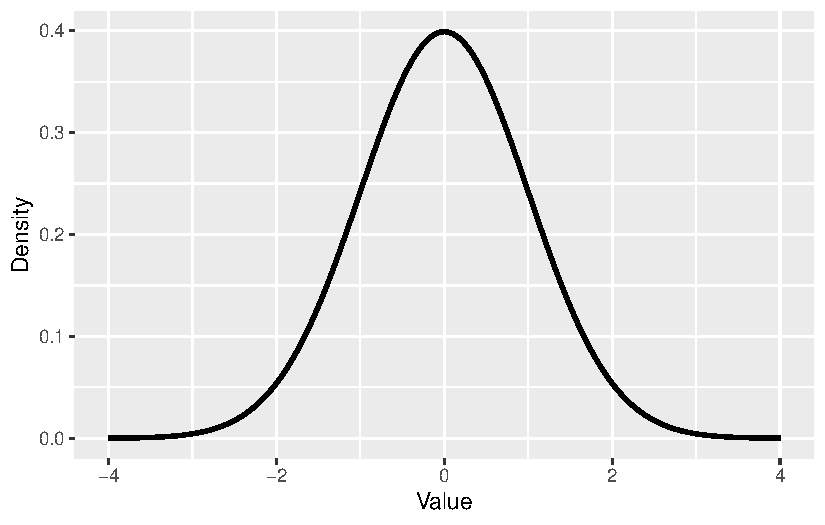
\includegraphics[keepaspectratio]{3_MeasurementError_files/figure-pdf/unnamed-chunk-27-1.pdf}}

But the bell curve did not first appear as a mysterious picture in a
statistics textbook. It emerged from a much older question:

\begin{quote}
What happens when we repeat a simple chance process many times?
\end{quote}

To see this, we return to games of chance.

Abraham de Moivre was born in France in 1667, but spent much of his
adult life in England. Like Pascal, Fermat, Huygens, and Bernoulli
before him, he belonged to the early history of probability, when many
of the central questions still came from gambling, wagers, annuities,
and games.

\begin{figure}[H]

{\centering 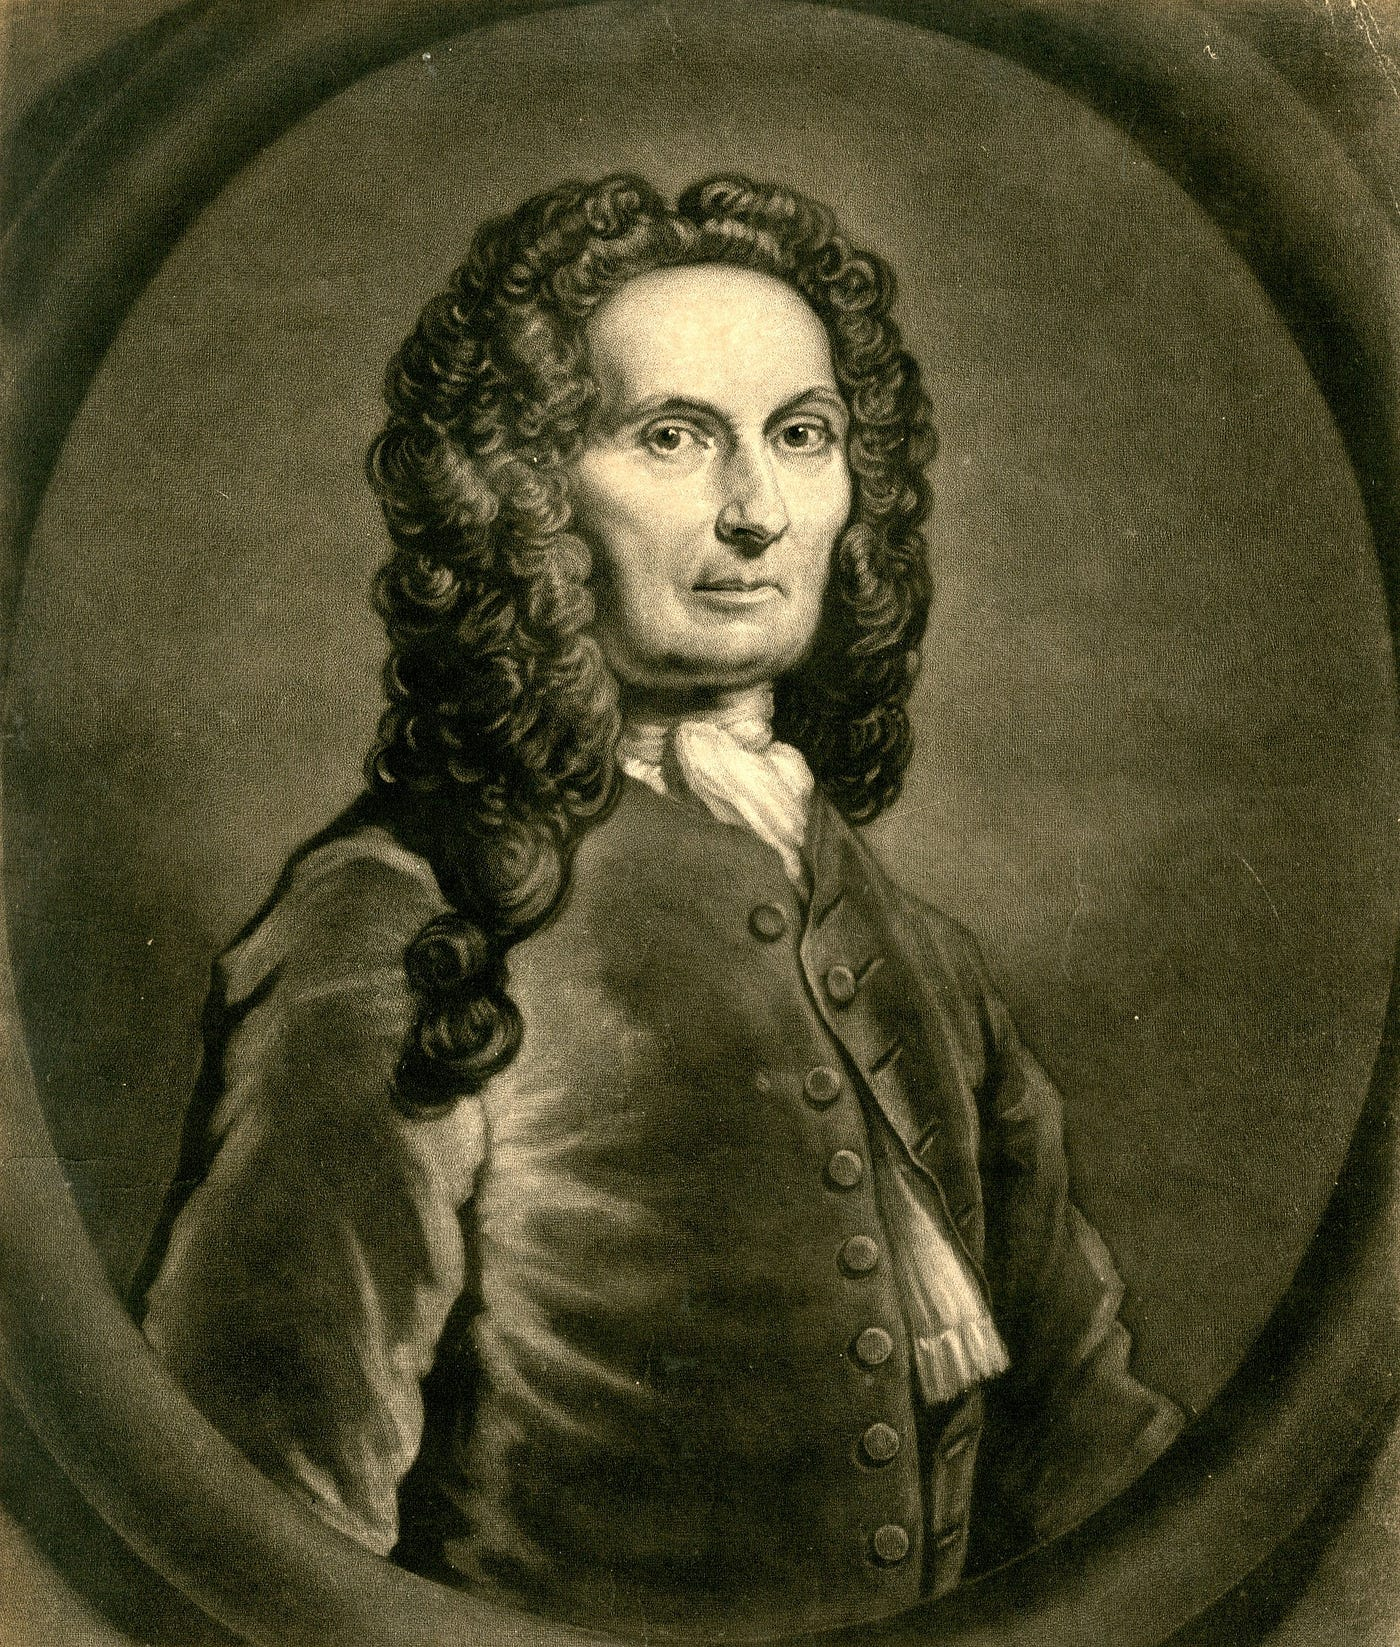
\includegraphics[width=0.5\linewidth,height=\textheight,keepaspectratio]{images/chapter3/demoivre.jpg}

}

\caption{Image Source:
https://en.wikipedia.org/wiki/Abraham\_de\_Moivre}

\end{figure}%

De Moivre was a gifted mathematician and a friend of Isaac Newton, but
his life was not especially secure. As a Protestant in Catholic France,
he left for England after the revocation of the Edict of Nantes. In
England, despite his brilliance, he never obtained the kind of
university position or official post that might have given him comfort.
He earned a living by tutoring mathematics, advising on annuities, and
solving probability problems for people who wanted answers about risk,
money, and chance.

This setting matters. Probability was not born as a purely abstract
subject. It grew out of practical questions:

\begin{quote}
What is a fair wager?
\end{quote}

\begin{quote}
How likely is a run of wins?
\end{quote}

\begin{quote}
How should we price an annuity?
\end{quote}

\begin{quote}
What should we expect after many repetitions of the same chance event?
\end{quote}

One of the simplest repeated chance events is the toss of a coin. If we
toss a fair coin once, there are two possible outcomes:

\[
H,\ T
\]

If we toss it twice, there are four possible sequences:

\[
HH,\ HT,\ TH,\ TT
\]

But now notice something important. If we care only about the number of
heads, the outcomes are not evenly distributed.

There is one way to get 0 heads:

\[
TT
\]

There are two ways to get 1 head:

\[
HT,\ TH
\]

There is one way to get 2 heads:

\[
HH
\]

So the counts are:

\[
1,\ 2,\ 1
\]

The middle outcome (one head) is already more common than the extremes,
not because the coin prefers balance, but because there are more ways to
get one head and one tail than to get all heads or all tails. If we toss
the coin three times, there are eight possible sequences:

\[
HHH,\ HHT,\ HTH,\ THH,\ HTT,\ THT,\ TTH,\ TTT
\]

Again, count the number of heads.

\pandocbounded{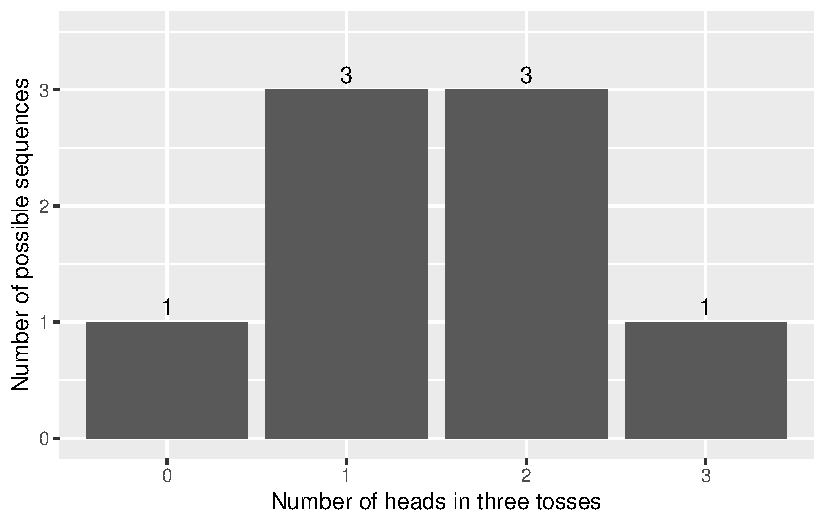
\includegraphics[keepaspectratio]{3_MeasurementError_files/figure-pdf/unnamed-chunk-29-1.pdf}}

These numbers should look familiar. They are rows of Pascal's triangle.

\begin{table}
\fontsize{12.0pt}{14.0pt}\selectfont
\begin{tabular*}{\linewidth}{@{\extracolsep{\fill}}rr}
\toprule
Number of coin tosses & Number of ways to get 0, 1, 2, ... heads \\ 
\midrule\addlinespace[2.5pt]
1 & 1, 1 \\ 
2 & 1, 2, 1 \\ 
3 & 1, 3, 3, 1 \\ 
4 & 1, 4, 6, 4, 1 \\ 
5 & 1, 5, 10, 10, 5, 1 \\ 
6 & 1, 6, 15, 20, 15, 6, 1 \\ 
\bottomrule
\end{tabular*}
\end{table}

Pascal's triangle tells us how many ways each number of heads can occur.
The extremes are rare because they can happen in only one way. There is
only one sequence with all heads and only one sequence with all tails.
The middle outcomes are common because they can happen in many different
ways.

For example, with 6 tosses, there is only one way to get 6 heads:

\[
HHHHHH
\]

There is also only one way to get 0 heads:

\[
TTTTTT
\]

But there are 20 ways to get exactly 3 heads. The centre is more
crowded.

\pandocbounded{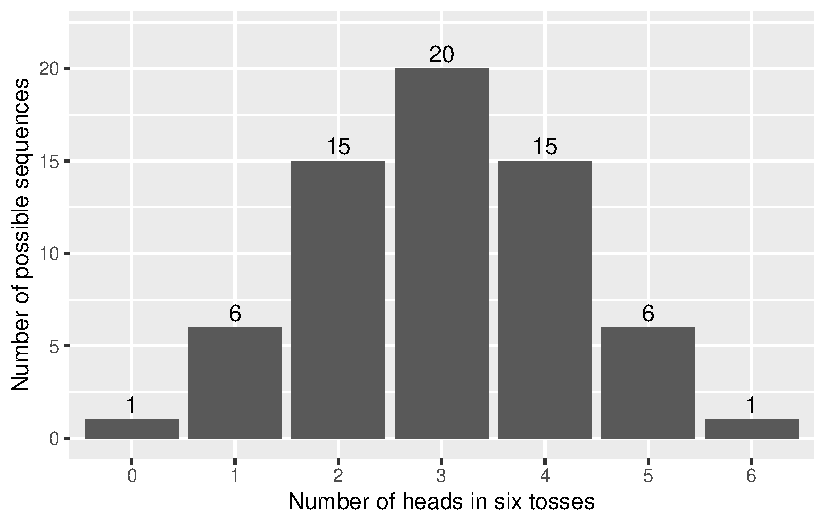
\includegraphics[keepaspectratio]{3_MeasurementError_files/figure-pdf/unnamed-chunk-31-1.pdf}}

This simple counting fact is the beginning of the bell curve. At first,
with only a few tosses, the pattern is jagged. We just see a short row
of numbers. But as the number of tosses grows, the shape becomes
clearer. The counts pile up near the centre and thin out toward the
extremes.

Imagine tossing a fair coin 20 times. The most likely result is not 20
heads or 0 heads. Those are possible, but each can happen in only one
way. The most likely results are near 10 heads and 10 tails, because
there are many more ways for that balance to occur.

\begin{table}
\fontsize{12.0pt}{14.0pt}\selectfont
\begin{tabular*}{\linewidth}{@{\extracolsep{\fill}}rrr}
\toprule
Number of heads in 20 tosses & Number of ways & Probability \\ 
\midrule\addlinespace[2.5pt]
0 & 1 & 0.00000 \\ 
1 & 20 & 0.00002 \\ 
2 & 190 & 0.00018 \\ 
3 & 1140 & 0.00109 \\ 
4 & 4845 & 0.00462 \\ 
5 & 15504 & 0.01479 \\ 
6 & 38760 & 0.03696 \\ 
7 & 77520 & 0.07393 \\ 
8 & 125970 & 0.12013 \\ 
9 & 167960 & 0.16018 \\ 
10 & 184756 & 0.17620 \\ 
11 & 167960 & 0.16018 \\ 
12 & 125970 & 0.12013 \\ 
13 & 77520 & 0.07393 \\ 
14 & 38760 & 0.03696 \\ 
15 & 15504 & 0.01479 \\ 
16 & 4845 & 0.00462 \\ 
17 & 1140 & 0.00109 \\ 
18 & 190 & 0.00018 \\ 
19 & 20 & 0.00002 \\ 
20 & 1 & 0.00000 \\ 
\bottomrule
\end{tabular*}
\end{table}

The table contains the arithmetic, but the shape is easier to see in a
graph.

\pandocbounded{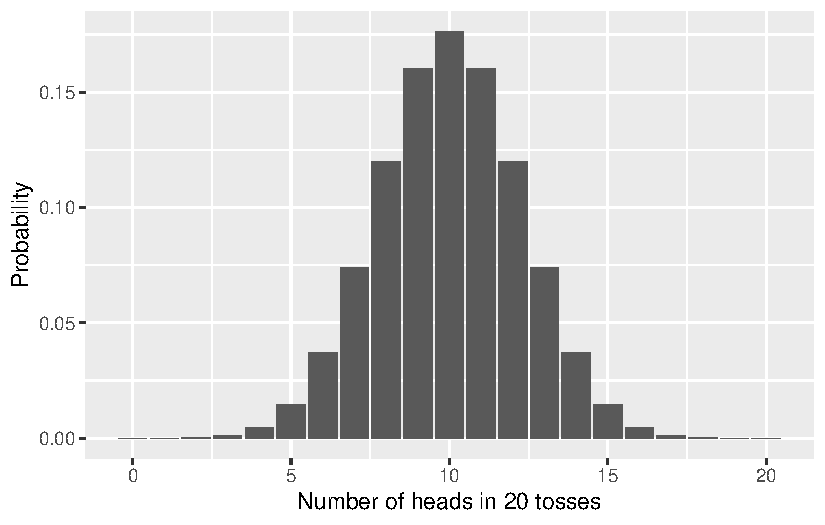
\includegraphics[keepaspectratio]{3_MeasurementError_files/figure-pdf/unnamed-chunk-33-1.pdf}}

The bars rise toward the middle and fall away toward the edges. The
distribution is symmetric because heads and tails are equally likely. It
is centred at 10 because, in 20 fair tosses, 10 heads is the balancing
point.

Now increase the number of tosses to 100.

\pandocbounded{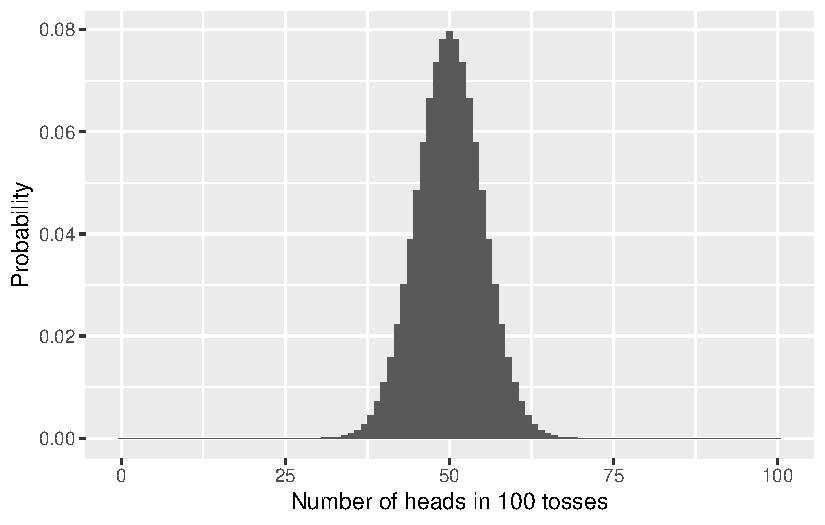
\includegraphics[keepaspectratio]{3_MeasurementError_files/figure-pdf/unnamed-chunk-34-1.pdf}}

The same basic pattern appears, but now it looks smoother. The
distribution rises to a peak near 50 and then falls away on both sides.
Values near the centre are common. Values far from the centre are rare.

This is the shape de Moivre studied. In 1733, de Moivre found a
remarkable approximation. He showed that, when the number of trials is
large, the jagged probabilities from repeated coin tossing can be
approximated by a smooth curve. That curve rises in the middle and falls
away on both sides. Today, we recognise this as an early form of the
normal curve, or bell curve.

This was an important step in the history of probability. De Moivre
showed that a pattern built from discrete counts could be approximated
by a continuous curve. A row of separate probabilities could be
replaced, approximately, by a smooth mathematical shape.

A single coin toss is only heads or tails. But many coin tosses,
gathered together, produce a shape. One toss gives randomness. Many
tosses give structure. We can see this by comparing several
distributions.

\pandocbounded{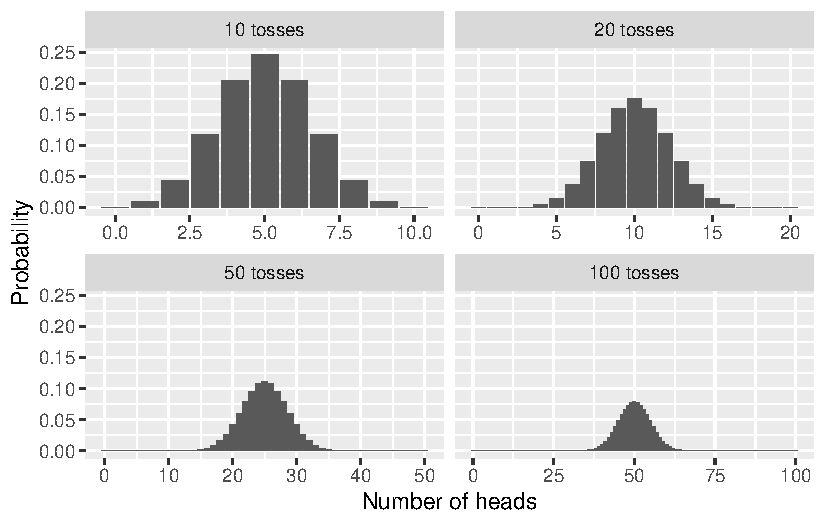
\includegraphics[keepaspectratio]{3_MeasurementError_files/figure-pdf/unnamed-chunk-35-1.pdf}}

With 10 tosses, the pattern is still rough. With 20 tosses, the mound is
clearer. With 50 or 100 tosses, the distribution increasingly resembles
a smooth bell. The reason is simple but powerful:

\begin{quote}
There are many ways to be near the centre, and very few ways to be
extreme.
\end{quote}

In 100 fair coin tosses, getting exactly 100 heads requires one very
special sequence:

\[
HHHHHHHHHH \cdots H
\]

Getting exactly 0 heads also requires one very special sequence:

\[
TTTTTTTTTT \cdots T
\]

But getting close to 50 heads can happen in an enormous number of
different orders. The heads and tails can be mixed in countless ways.
The centre is crowded because many paths lead there. The extremes are
lonely because very few paths reach them. This gives us an intuitive way
to understand the bell curve:

\begin{quote}
The bell curve appears when many small sources of variation combine, and
there are many more ways to end up near the centre than far from it.
\end{quote}

Now we can connect de Moivre back to measurement. A repeated measurement
is not the same as a coin toss, but the underlying logic is similar. A
measurement can be pushed slightly upward or downward by many small
influences. A wine score might be affected by the order of tasting, the
temperature of the wine, the glassware, the critic's expectations, the
food eaten beforehand, and the critic's mood. An exam mark might be
affected by preparation, sleep, question wording, time pressure, nerves,
marking judgement, and chance. A physical measurement might be affected
by instrument precision, calibration, temperature, vibration, rounding,
and the observer's judgement.

Each influence may be small. Some push the measurement upward. Others
push it downward. Often, they partly cancel out. When they do, the
result stays near the centre. A very large error requires many
influences to push in the same direction at once, just as getting 100
heads requires every toss to land the same way. This is why the bell
curve became so important. It gave mathematicians and scientists a way
to describe variation, not as shapeless disorder, but as patterned
uncertainty. At the same time, we should be careful. Not everything
follows a bell curve. Many real datasets are skewed, uneven, or shaped
by social forces, physical limits, or feedback loops. Incomes, house
prices, waiting times, social media followers, and city sizes often do
not form neat bell-shaped patterns.

The bell curve is not a universal law of data. But it is a remarkably
useful model for many situations involving repeated measurement and many
small sources of variation. It helps us understand why values often
cluster near an average, why extreme values are rarer, and why variation
can have a predictable shape.

\section{Gauss and the normal
distribution}\label{gauss-and-the-normal-distribution}

De Moivre showed that a bell-shaped curve could emerge from repeated
chance. Many coin tosses, counted carefully, produced a pattern: results
near the centre were common, and results far from the centre were rare.

But the bell curve became truly central to statistics when it moved from
games of chance into the problem of measurement. This brings us to Carl
Friedrich Gauss.

\begin{figure}[H]

{\centering 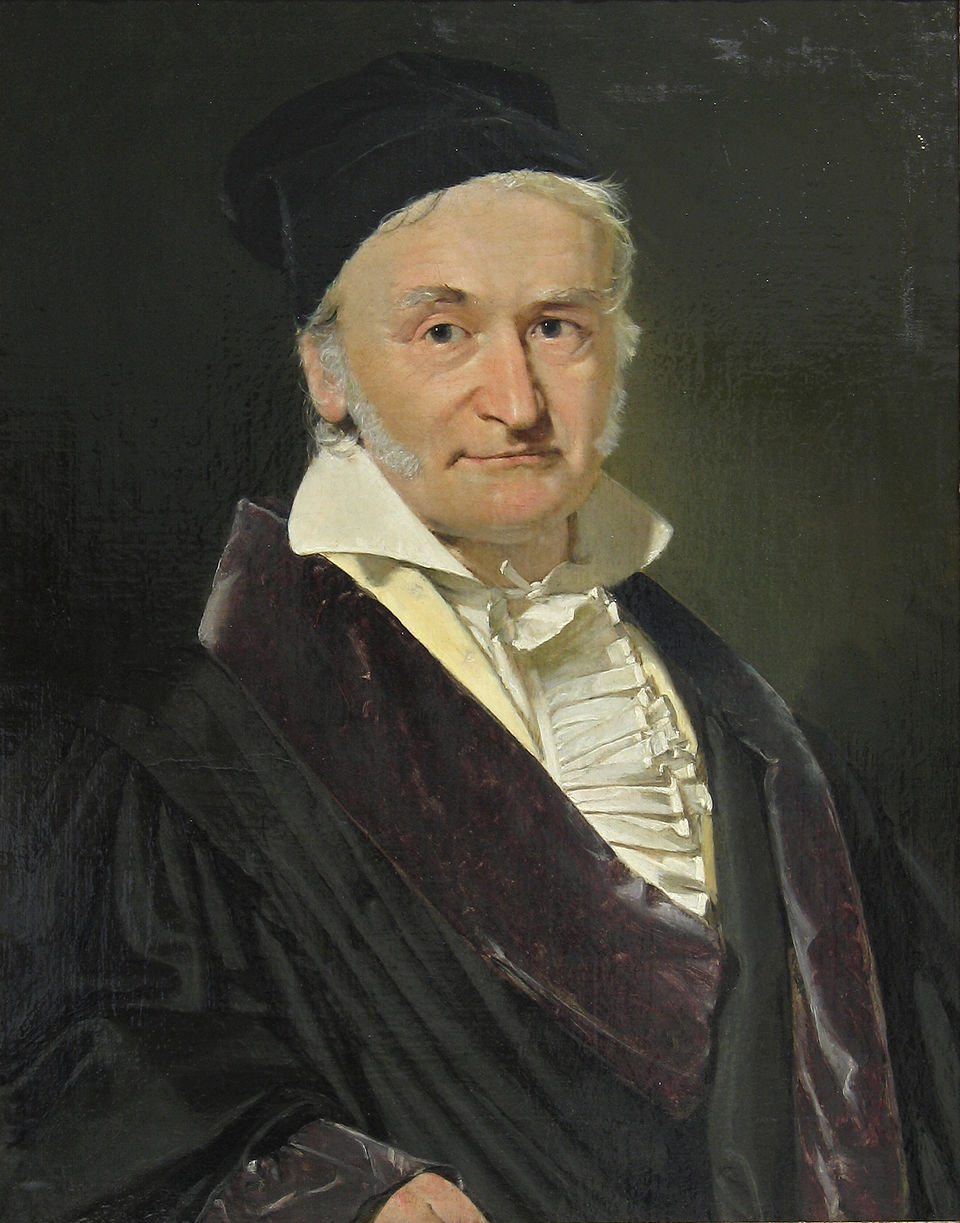
\includegraphics[width=3.2in,height=\textheight,keepaspectratio]{images/chapter3/Gauss.jpg}

}

\caption{Portrait of Carl Friedrich Gauss by Christian Albrecht Jensen}

\end{figure}%

Gauss was born in Germany in 1777 and is often described as one of the
greatest mathematicians in history. Stories about his talent begin when
he was a child. One famous story says that when his schoolteacher asked
the class to add the numbers from 1 to 100, hoping to keep them busy,
Gauss quickly noticed a shortcut. Pair the first and last numbers:

\[
1 + 100 = 101
\]

Then:

\[
2 + 99 = 101
\]

And:

\[
3 + 98 = 101
\]

There are 50 such pairs, so the total is:

\[
50 \times 101 = 5050
\]

Whether or not the story happened exactly this way, it captures
something true about Gauss's reputation. He had an extraordinary ability
to see structure where others saw only tedious calculation. That ability
mattered because Gauss worked in a world where measurement was becoming
increasingly important. Astronomers were tracking planets, comets, and
stars. Surveyors were measuring land. Scientists were using instruments
to record physical quantities. But repeated measurements rarely agreed
perfectly.

An astronomer might measure the position of a planet several times and
obtain slightly different answers. A surveyor might measure an angle and
find that repeated readings disagree by a small amount. A physicist
might measure the same quantity again and again, only to find that the
last decimal place keeps changing.

The question was not merely:

\begin{quote}
What is the measurement?
\end{quote}

The question was:

\begin{quote}
Given several imperfect measurements, what is our best estimate of the
true value?
\end{quote}

This is the measurement problem at the heart of this chapter. Suppose we
are trying to measure a true value. We do not see the true value
directly. Instead, we observe measurements that contain error:

\[
\text{Observed value} = \text{True value} + \text{Error}
\]

If the errors are random and balanced, some measurements will be too
high and some will be too low. Most errors will be small. Large errors
will be less common. Very large errors will be rare.

That is exactly the shape we have been building toward. The bell curve
gives us a way to describe this pattern. Today, we usually call this
curve the \textbf{normal distribution}. Its familiar shape is symmetric,
highest in the middle, and tapering toward both ends.

The normal distribution is usually described using two quantities:

\[
\mu
\quad \text{and} \quad
\sigma
\]

The symbol \(\mu\) represents the centre, or mean. The symbol \(\sigma\)
represents the spread, or standard deviation.

We write:

\[
X \sim N(\mu, \sigma)
\]

This is read as:

\begin{quote}
\begin{enumerate}
\def\labelenumi{(\Alph{enumi})}
\setcounter{enumi}{23}
\tightlist
\item
  follows a normal distribution with mean \(\mu\) and standard deviation
  \(\sigma\)
\end{enumerate}
\end{quote}

The mean tells us where the curve is centred. The standard deviation
tells us how spread out the curve is. A normal distribution with a small
standard deviation is tightly clustered around the mean. A normal
distribution with a large standard deviation is more spread out.

\pandocbounded{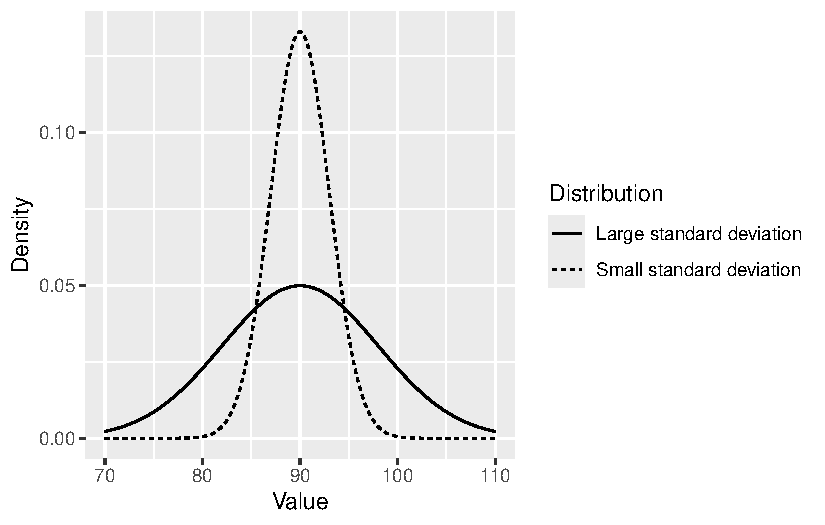
\includegraphics[keepaspectratio]{3_MeasurementError_files/figure-pdf/unnamed-chunk-37-1.pdf}}

Both curves are centred at 90. But they tell very different stories. In
the narrow curve, values close to 90 are very common, and values far
from 90 are rare. In the wider curve, values are more spread out. A
value of 80 or 100 is no longer so surprising.

Let's revisit the wine example. Suppose two wines both have an average
rating of 90.

\begin{itemize}
\tightlist
\item
  If Wine A has a standard deviation of 2, critics mostly agree.
\item
  If Wine B has a standard deviation of 8, critics disagree much more.
\end{itemize}

The average rating alone says both wines are 90-point wines. The
standard deviation tells us whether that average is stable or uncertain.
This is why the normal distribution is so useful for thinking about
measurement. It does not merely tell us the centre. It tells us how
observations are likely to vary around that centre.

For example, suppose repeated ratings of a wine are approximately normal
with mean 90 and standard deviation 2:

\[
X \sim N(90, 2)
\]

Then ratings near 90 are common. Ratings such as 89, 90, and 91 would
not surprise us. Ratings such as 84 or 96 would be much less common.

Now suppose another wine has ratings that are approximately normal with
mean 90 and standard deviation 8:

\[
X \sim N(90, 8)
\]

Now ratings far from 90 are much more plausible. A critic giving 82 or
98 would not be nearly as surprising. The mean is the same. The
uncertainty is not.

Gauss's connection to this curve came through the problem of errors. If
many small, independent sources of error affect a measurement, and if
those errors tend to balance around zero, then the resulting
measurements often cluster around the true value in a bell-shaped
pattern. In that setting, the centre of the curve represents the true
value, or our best estimate of it. The spread of the curve represents
measurement error. This is sometimes called the \textbf{law of error}.

The phrase can sound grand, but the intuition is simple. If a
measurement is affected by many small accidental influences, then most
measurements should be close to the truth. Occasionally, several
influences will push in the same direction and the error will be larger.
Very large errors should be rare.

Imagine measuring the same object 100 times. If the true value is 50,
and the measurement errors are small and balanced, the observed values
might look like this:

\pandocbounded{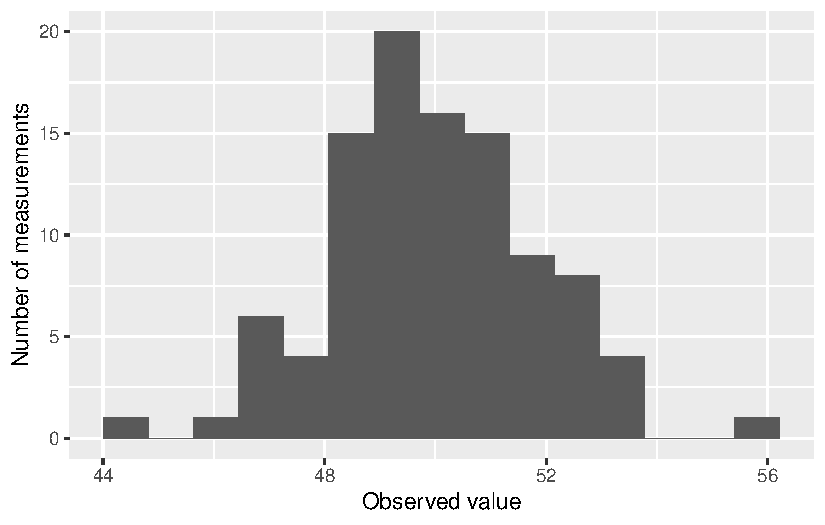
\includegraphics[keepaspectratio]{3_MeasurementError_files/figure-pdf/unnamed-chunk-38-1.pdf}}

The histogram will not be perfectly smooth. Real data rarely are. But
the general pattern should be visible: many observations near 50, fewer
observations farther away.

This is the bell curve in measurement form.

Now compare two measurement processes. Both are centred around the same
true value, 50. But one process has small error and the other has larger
error.

\pandocbounded{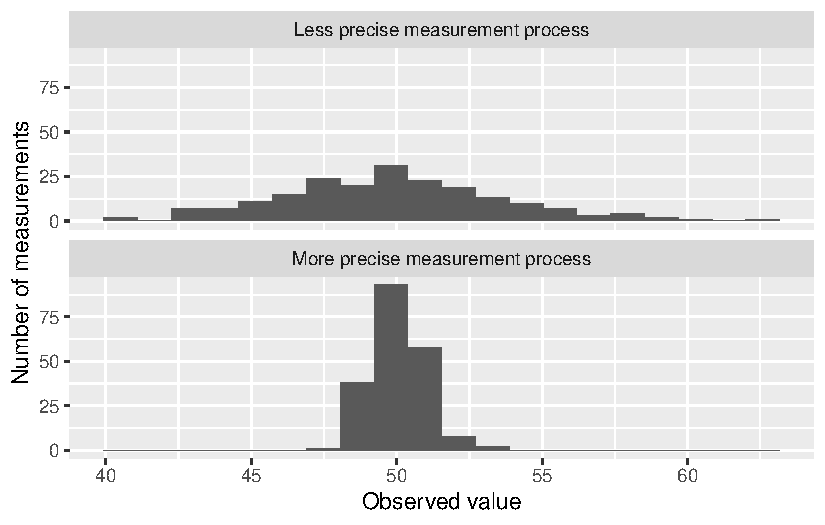
\includegraphics[keepaspectratio]{3_MeasurementError_files/figure-pdf/unnamed-chunk-39-1.pdf}}

The first measurement process produces values tightly clustered around
50. The second produces values spread more widely. Both may be centred
correctly, but they are not equally precise.

This lets us distinguish two ideas that are often confused:

\begin{itemize}
\tightlist
\item
  \textbf{Accuracy}: whether measurements are centred around the true
  value.
\item
  \textbf{Precision}: how tightly repeated measurements cluster
  together.
\end{itemize}

A measurement process can be accurate but not very precise. It can be
precise but not accurate. Ideally, we want both.

\begin{table}
\fontsize{12.0pt}{14.0pt}\selectfont
\begin{tabular*}{\linewidth}{@{\extracolsep{\fill}}lll}
\toprule
Pattern & Meaning & Example \\ 
\midrule\addlinespace[2.5pt]
Accurate and precise & Measurements cluster tightly around the true value & A well-calibrated instrument with little noise \\ 
Accurate but not precise & Measurements are spread out but centred correctly & A noisy instrument that is correct on average \\ 
Precise but not accurate & Measurements cluster tightly around the wrong value & A miscalibrated instrument that gives consistent but biased readings \\ 
Neither accurate nor precise & Measurements are spread out and off-centre & A poor instrument with both bias and noise \\ 
\bottomrule
\end{tabular*}
\end{table}

The normal distribution gives us one way to describe this uncertainty.
It says: do not look only at the observed value. Ask how much variation
surrounds it. This is why the bell curve became so deeply connected to
statistics. It joined three ideas that have been running through the
chapter:

\begin{enumerate}
\def\labelenumi{\arabic{enumi}.}
\tightlist
\item
  \textbf{A centre}: values tend to cluster around some typical value.
\item
  \textbf{Variation}: observations differ from that centre.
\item
  \textbf{Pattern}: the variation is not always shapeless; it may follow
  a predictable form.
\end{enumerate}

The normal distribution is not the only distribution in statistics (more
on this in Chapter 7). It is not always appropriate. We should not force
a bell curve onto every dataset simply because it is familiar. But when
a quantity is shaped by many small, roughly independent influences, and
when those influences push in both directions, the normal distribution
is often a useful starting point.

\section{Coding the ideas in R}\label{coding-the-ideas-in-r-2}

Throughout this chapter, we have treated data as the result of a
measurement process. A number may look exact, but it may contain random
error, systematic error, or both. We have also seen that repeated
observations can reveal patterns, while small samples can mislead us.

We can use R to code these ideas directly.

The goal of this section is not to replace the reasoning from the
chapter. The goal is to show how the same ideas can be expressed in
code. This is useful because code allows us to simulate measurement
processes, repeat them many times, and see how variation behaves.

\subsection{Simulating random and systematic
error}\label{simulating-random-and-systematic-error}

A useful way to think about measurement is:

\[
\text{Observed value} = \text{True value} + \text{Error}
\]

In this chapter, we separated error into two parts:

\[
\text{Observed value}
=
\text{True value}
+
\text{Systematic error}
+
\text{Random error}
\]

We can simulate this idea in R.

Suppose the true value of an object is 100. We measure it 30 times. The
measurement device has small random error, but no systematic error.

\begin{Shaded}
\begin{Highlighting}[]
\FunctionTok{set.seed}\NormalTok{(}\DecValTok{24205242}\NormalTok{)}

\NormalTok{random\_error\_measurements }\OtherTok{\textless{}{-}} \FunctionTok{tibble}\NormalTok{(}
  \AttributeTok{measurement =} \DecValTok{1}\SpecialCharTok{:}\DecValTok{30}\NormalTok{,}
  \AttributeTok{true\_value =} \DecValTok{100}\NormalTok{,}
  \AttributeTok{systematic\_error =} \DecValTok{0}\NormalTok{,}
  \AttributeTok{random\_error =} \FunctionTok{rnorm}\NormalTok{(}\AttributeTok{n =} \DecValTok{30}\NormalTok{, }\AttributeTok{mean =} \DecValTok{0}\NormalTok{, }\AttributeTok{sd =} \DecValTok{2}\NormalTok{),}
  \AttributeTok{observed\_value =}\NormalTok{ true\_value }\SpecialCharTok{+}\NormalTok{ systematic\_error }\SpecialCharTok{+}\NormalTok{ random\_error}
\NormalTok{)}

\NormalTok{random\_error\_measurements}
\end{Highlighting}
\end{Shaded}

\begin{verbatim}
# A tibble: 30 x 5
   measurement true_value systematic_error random_error observed_value
         <int>      <dbl>            <dbl>        <dbl>          <dbl>
 1           1        100                0        1.06           101. 
 2           2        100                0        3.68           104. 
 3           3        100                0       -1.48            98.5
 4           4        100                0        2.14           102. 
 5           5        100                0       -2.76            97.2
 6           6        100                0        2.04           102. 
 7           7        100                0       -0.248           99.8
 8           8        100                0       -5.58            94.4
 9           9        100                0        3.16           103. 
10          10        100                0        0.567          101. 
# i 20 more rows
\end{verbatim}

The function \texttt{rnorm()} generates random numbers from a normal
distribution.

In this example:

\begin{itemize}
\tightlist
\item
  \texttt{n\ =\ 30} means we generate 30 random errors,
\item
  \texttt{mean\ =\ 0} means the random errors are centred around zero,
\item
  \texttt{sd\ =\ 2} means the random errors typically vary by about 2
  units.
\end{itemize}

We can summarise the observed measurements.

\begin{Shaded}
\begin{Highlighting}[]
\NormalTok{random\_error\_measurements }\SpecialCharTok{|\textgreater{}}
  \FunctionTok{summarise}\NormalTok{(}
    \AttributeTok{mean\_observed =} \FunctionTok{mean}\NormalTok{(observed\_value),}
    \AttributeTok{sd\_observed =} \FunctionTok{sd}\NormalTok{(observed\_value),}
    \AttributeTok{minimum =} \FunctionTok{min}\NormalTok{(observed\_value),}
    \AttributeTok{maximum =} \FunctionTok{max}\NormalTok{(observed\_value)}
\NormalTok{  )}
\end{Highlighting}
\end{Shaded}

\begin{verbatim}
# A tibble: 1 x 4
  mean_observed sd_observed minimum maximum
          <dbl>       <dbl>   <dbl>   <dbl>
1          100.        2.03    94.4    104.
\end{verbatim}

The mean observed value should be close to 100, because the random
errors are centred around zero. The individual measurements vary, but
they do not consistently lean upward or downward.

Now suppose the measurement device is biased upward by 5 units. This is
systematic error.

\begin{Shaded}
\begin{Highlighting}[]
\FunctionTok{set.seed}\NormalTok{(}\DecValTok{24205242}\NormalTok{)}

\NormalTok{systematic\_error\_measurements }\OtherTok{\textless{}{-}} \FunctionTok{tibble}\NormalTok{(}
  \AttributeTok{measurement =} \DecValTok{1}\SpecialCharTok{:}\DecValTok{30}\NormalTok{,}
  \AttributeTok{true\_value =} \DecValTok{100}\NormalTok{,}
  \AttributeTok{systematic\_error =} \DecValTok{5}\NormalTok{,}
  \AttributeTok{random\_error =} \FunctionTok{rnorm}\NormalTok{(}\AttributeTok{n =} \DecValTok{30}\NormalTok{, }\AttributeTok{mean =} \DecValTok{0}\NormalTok{, }\AttributeTok{sd =} \DecValTok{2}\NormalTok{),}
  \AttributeTok{observed\_value =}\NormalTok{ true\_value }\SpecialCharTok{+}\NormalTok{ systematic\_error }\SpecialCharTok{+}\NormalTok{ random\_error}
\NormalTok{)}

\NormalTok{systematic\_error\_measurements}
\end{Highlighting}
\end{Shaded}

\begin{verbatim}
# A tibble: 30 x 5
   measurement true_value systematic_error random_error observed_value
         <int>      <dbl>            <dbl>        <dbl>          <dbl>
 1           1        100                5        1.06           106. 
 2           2        100                5        3.68           109. 
 3           3        100                5       -1.48           104. 
 4           4        100                5        2.14           107. 
 5           5        100                5       -2.76           102. 
 6           6        100                5        2.04           107. 
 7           7        100                5       -0.248          105. 
 8           8        100                5       -5.58            99.4
 9           9        100                5        3.16           108. 
10          10        100                5        0.567          106. 
# i 20 more rows
\end{verbatim}

The random error is the same kind of noise as before, but the
measurements are now centred around the wrong value.

We can compare the two measurement processes.

\begin{Shaded}
\begin{Highlighting}[]
\NormalTok{measurement\_comparison }\OtherTok{\textless{}{-}} \FunctionTok{bind\_rows}\NormalTok{(}
\NormalTok{  random\_error\_measurements }\SpecialCharTok{|\textgreater{}}
    \FunctionTok{mutate}\NormalTok{(}\AttributeTok{process =} \StringTok{"Random error only"}\NormalTok{),}
\NormalTok{  systematic\_error\_measurements }\SpecialCharTok{|\textgreater{}}
    \FunctionTok{mutate}\NormalTok{(}\AttributeTok{process =} \StringTok{"Random error plus systematic error"}\NormalTok{)}
\NormalTok{)}

\NormalTok{measurement\_comparison }\SpecialCharTok{|\textgreater{}}
  \FunctionTok{group\_by}\NormalTok{(process) }\SpecialCharTok{|\textgreater{}}
  \FunctionTok{summarise}\NormalTok{(}
    \AttributeTok{mean\_observed =} \FunctionTok{mean}\NormalTok{(observed\_value),}
    \AttributeTok{sd\_observed =} \FunctionTok{sd}\NormalTok{(observed\_value),}
    \AttributeTok{.groups =} \StringTok{"drop"}
\NormalTok{  )}
\end{Highlighting}
\end{Shaded}

\begin{verbatim}
# A tibble: 2 x 3
  process                            mean_observed sd_observed
  <chr>                                      <dbl>       <dbl>
1 Random error only                           100.        2.03
2 Random error plus systematic error          105.        2.03
\end{verbatim}

The function \texttt{bind\_rows()} stacks two data frames on top of each
other. The function \texttt{group\_by()} tells R to calculate the
summary separately for each measurement process.

We can also plot the measurements.

\begin{Shaded}
\begin{Highlighting}[]
\NormalTok{measurement\_comparison }\SpecialCharTok{|\textgreater{}}
  \FunctionTok{ggplot}\NormalTok{(}\FunctionTok{aes}\NormalTok{(}\AttributeTok{x =}\NormalTok{ measurement, }\AttributeTok{y =}\NormalTok{ observed\_value)) }\SpecialCharTok{+}
  \FunctionTok{geom\_point}\NormalTok{() }\SpecialCharTok{+}
  \FunctionTok{geom\_hline}\NormalTok{(}\AttributeTok{yintercept =} \DecValTok{100}\NormalTok{, }\AttributeTok{linetype =} \StringTok{"dashed"}\NormalTok{) }\SpecialCharTok{+}
  \FunctionTok{facet\_wrap}\NormalTok{(}\SpecialCharTok{\textasciitilde{}}\NormalTok{ process) }\SpecialCharTok{+}
  \FunctionTok{labs}\NormalTok{(}
    \AttributeTok{x =} \StringTok{"Measurement number"}\NormalTok{,}
    \AttributeTok{y =} \StringTok{"Observed value"}
\NormalTok{  )}
\end{Highlighting}
\end{Shaded}

\begin{figure}[H]

\centering{

\pandocbounded{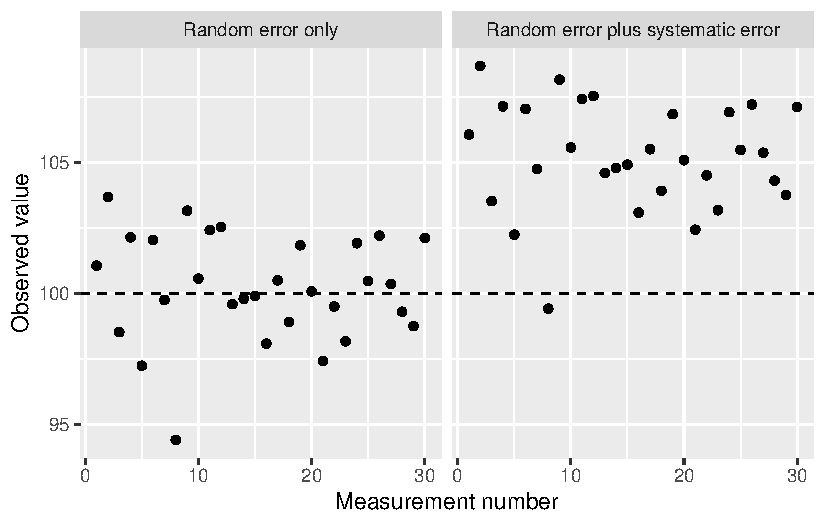
\includegraphics[keepaspectratio]{3_MeasurementError_files/figure-pdf/fig-random-systematic-error-1.pdf}}

}

\caption{\label{fig-random-systematic-error}Repeated measurements with
and without systematic error}

\end{figure}%

The dashed line shows the true value. In the random-error-only case, the
observations jump around the true value. In the systematic-error case,
the observations still jump around, but they are centred too high.

\subsection{Simulating the law of large
numbers}\label{simulating-the-law-of-large-numbers}

The law of large numbers says that short-run results may jump around,
but long-run proportions tend to stabilise.

Suppose a box contains red and blue balls. The probability of drawing a
red ball is 0.6. We draw one ball, record its colour, put it back, and
repeat this many times.

We can simulate this in R.

\begin{Shaded}
\begin{Highlighting}[]
\FunctionTok{set.seed}\NormalTok{(}\DecValTok{24205242}\NormalTok{)}

\NormalTok{n\_draws }\OtherTok{\textless{}{-}} \DecValTok{1000}

\NormalTok{urn\_draws }\OtherTok{\textless{}{-}} \FunctionTok{tibble}\NormalTok{(}
  \AttributeTok{draw =} \DecValTok{1}\SpecialCharTok{:}\NormalTok{n\_draws,}
  \AttributeTok{colour =} \FunctionTok{sample}\NormalTok{(}
    \AttributeTok{x =} \FunctionTok{c}\NormalTok{(}\StringTok{"Red"}\NormalTok{, }\StringTok{"Blue"}\NormalTok{),}
    \AttributeTok{size =}\NormalTok{ n\_draws,}
    \AttributeTok{replace =} \ConstantTok{TRUE}\NormalTok{,}
    \AttributeTok{prob =} \FunctionTok{c}\NormalTok{(}\FloatTok{0.6}\NormalTok{, }\FloatTok{0.4}\NormalTok{)}
\NormalTok{  )}
\NormalTok{)}

\NormalTok{urn\_draws}
\end{Highlighting}
\end{Shaded}

\begin{verbatim}
# A tibble: 1,000 x 2
    draw colour
   <int> <chr> 
 1     1 Blue  
 2     2 Red   
 3     3 Blue  
 4     4 Red   
 5     5 Red   
 6     6 Red   
 7     7 Blue  
 8     8 Red   
 9     9 Red   
10    10 Blue  
# i 990 more rows
\end{verbatim}

The function \texttt{sample()} randomly samples values from a set.

Here:

\begin{itemize}
\tightlist
\item
  \texttt{x\ =\ c("Red",\ "Blue")} gives the possible outcomes,
\item
  \texttt{size\ =\ n\_draws} says how many draws to make,
\item
  \texttt{replace\ =\ TRUE} means each ball is replaced before the next
  draw,
\item
  \texttt{prob\ =\ c(0.6,\ 0.4)} gives the probabilities of red and
  blue.
\end{itemize}

Now we calculate the running proportion of red balls.

\begin{Shaded}
\begin{Highlighting}[]
\NormalTok{urn\_draws }\OtherTok{\textless{}{-}}\NormalTok{ urn\_draws }\SpecialCharTok{|\textgreater{}}
  \FunctionTok{mutate}\NormalTok{(}
    \AttributeTok{red\_so\_far =} \FunctionTok{cumsum}\NormalTok{(colour }\SpecialCharTok{==} \StringTok{"Red"}\NormalTok{),}
    \AttributeTok{proportion\_red =}\NormalTok{ red\_so\_far }\SpecialCharTok{/}\NormalTok{ draw}
\NormalTok{  )}

\NormalTok{urn\_draws}
\end{Highlighting}
\end{Shaded}

\begin{verbatim}
# A tibble: 1,000 x 4
    draw colour red_so_far proportion_red
   <int> <chr>       <int>          <dbl>
 1     1 Blue            0          0    
 2     2 Red             1          0.5  
 3     3 Blue            1          0.333
 4     4 Red             2          0.5  
 5     5 Red             3          0.6  
 6     6 Red             4          0.667
 7     7 Blue            4          0.571
 8     8 Red             5          0.625
 9     9 Red             6          0.667
10    10 Blue            6          0.6  
# i 990 more rows
\end{verbatim}

The expression \texttt{colour\ ==\ "Red"} returns \texttt{TRUE} when the
draw is red and \texttt{FALSE} otherwise. In R, \texttt{TRUE} is treated
as 1 and \texttt{FALSE} is treated as 0. So
\texttt{cumsum(colour\ ==\ "Red")} counts how many red balls have
appeared so far.

We can plot the running proportion.

\begin{Shaded}
\begin{Highlighting}[]
\NormalTok{urn\_draws }\SpecialCharTok{|\textgreater{}}
  \FunctionTok{ggplot}\NormalTok{(}\FunctionTok{aes}\NormalTok{(}\AttributeTok{x =}\NormalTok{ draw, }\AttributeTok{y =}\NormalTok{ proportion\_red)) }\SpecialCharTok{+}
  \FunctionTok{geom\_line}\NormalTok{() }\SpecialCharTok{+}
  \FunctionTok{geom\_hline}\NormalTok{(}\AttributeTok{yintercept =} \FloatTok{0.6}\NormalTok{, }\AttributeTok{linetype =} \StringTok{"dashed"}\NormalTok{) }\SpecialCharTok{+}
  \FunctionTok{labs}\NormalTok{(}
    \AttributeTok{x =} \StringTok{"Number of draws"}\NormalTok{,}
    \AttributeTok{y =} \StringTok{"Observed proportion of red balls"}
\NormalTok{  )}
\end{Highlighting}
\end{Shaded}

\begin{figure}[H]

\centering{

\pandocbounded{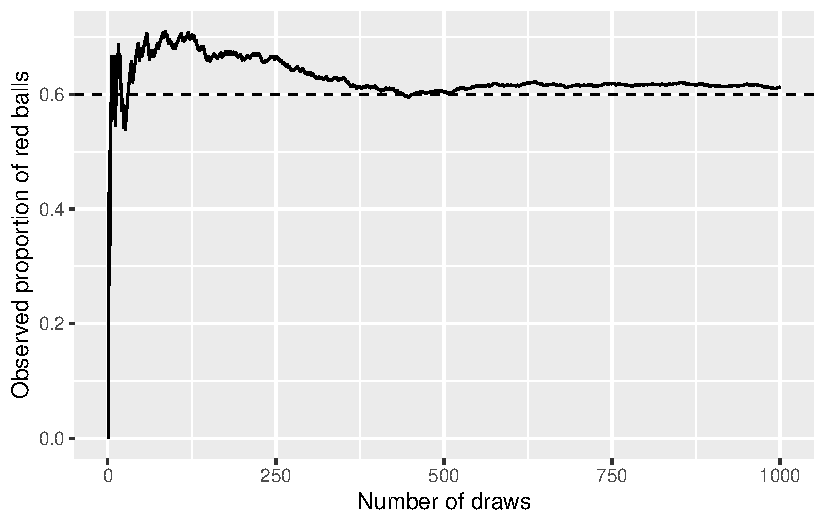
\includegraphics[keepaspectratio]{3_MeasurementError_files/figure-pdf/fig-law-large-numbers-1.pdf}}

}

\caption{\label{fig-law-large-numbers}The observed proportion of red
balls stabilises as the number of draws increases}

\end{figure}%

Early in the simulation, the observed proportion can move sharply. One
extra red or blue ball can make a large difference. Later, each new draw
has less influence on the accumulated proportion.

The dashed line marks the true probability:

\[
P(\text{red}) = 0.6.
\]

The observed proportion does not equal 0.6 at every moment. But as the
number of draws increases, it usually becomes more stable.

This is the law of large numbers in action.

\subsection{Seeing why small samples can
mislead}\label{seeing-why-small-samples-can-mislead}

The law of large numbers helps explain why large samples are often more
stable than small samples. The same observed proportion can mean
different things depending on how many observations it is based on.

Suppose a basketball player makes 8 out of 10 shots.

\begin{Shaded}
\begin{Highlighting}[]
\NormalTok{small\_sample }\OtherTok{\textless{}{-}} \FunctionTok{tibble}\NormalTok{(}
  \AttributeTok{shots\_taken =} \DecValTok{10}\NormalTok{,}
  \AttributeTok{shots\_made =} \DecValTok{8}\NormalTok{,}
  \AttributeTok{shooting\_percentage =}\NormalTok{ shots\_made }\SpecialCharTok{/}\NormalTok{ shots\_taken}
\NormalTok{)}

\NormalTok{small\_sample}
\end{Highlighting}
\end{Shaded}

\begin{verbatim}
# A tibble: 1 x 3
  shots_taken shots_made shooting_percentage
        <dbl>      <dbl>               <dbl>
1          10          8                 0.8
\end{verbatim}

The shooting percentage is 80\%. But this is based on only 10 shots. A
short run can easily be affected by chance.

Now suppose a player makes 80 out of 100 shots.

\begin{Shaded}
\begin{Highlighting}[]
\NormalTok{larger\_sample }\OtherTok{\textless{}{-}} \FunctionTok{tibble}\NormalTok{(}
  \AttributeTok{shots\_taken =} \DecValTok{100}\NormalTok{,}
  \AttributeTok{shots\_made =} \DecValTok{80}\NormalTok{,}
  \AttributeTok{shooting\_percentage =}\NormalTok{ shots\_made }\SpecialCharTok{/}\NormalTok{ shots\_taken}
\NormalTok{)}

\NormalTok{larger\_sample}
\end{Highlighting}
\end{Shaded}

\begin{verbatim}
# A tibble: 1 x 3
  shots_taken shots_made shooting_percentage
        <dbl>      <dbl>               <dbl>
1         100         80                 0.8
\end{verbatim}

The shooting percentage is still 80\%, but it is based on much more
information.

We can compare the two cases in one table.

\begin{table}

\caption{\label{tbl-small-large-samples}The same percentage can carry
different amounts of evidence}

\centering{

\fontsize{12.0pt}{14.0pt}\selectfont
\begin{tabular*}{\linewidth}{@{\extracolsep{\fill}}cccc}
\toprule
Situation & Shots made & Shots taken & Shooting percentage \\ 
\midrule\addlinespace[2.5pt]
Small sample & 8 & 10 & 80\% \\ 
Larger sample & 80 & 100 & 80\% \\ 
\bottomrule
\end{tabular*}

}

\end{table}%

Both rows show 80\%, but they should not be interpreted in the same way.
The larger sample gives stronger evidence about the player's long-run
shooting ability.

We can see this more directly by simulating many players who all have
the same true shooting probability.

Suppose the true probability of making a shot is 0.7. We simulate many
short samples of 10 shots, and many larger samples of 100 shots.

\begin{Shaded}
\begin{Highlighting}[]
\FunctionTok{set.seed}\NormalTok{(}\DecValTok{24205242}\NormalTok{)}

\NormalTok{n\_simulations }\OtherTok{\textless{}{-}} \DecValTok{5000}
\NormalTok{true\_probability }\OtherTok{\textless{}{-}} \FloatTok{0.7}

\NormalTok{shooting\_simulations }\OtherTok{\textless{}{-}} \FunctionTok{bind\_rows}\NormalTok{(}
  \FunctionTok{tibble}\NormalTok{(}
    \AttributeTok{simulation =} \DecValTok{1}\SpecialCharTok{:}\NormalTok{n\_simulations,}
    \AttributeTok{shots\_taken =} \DecValTok{10}\NormalTok{,}
    \AttributeTok{shots\_made =} \FunctionTok{rbinom}\NormalTok{(}
      \AttributeTok{n =}\NormalTok{ n\_simulations,}
      \AttributeTok{size =} \DecValTok{10}\NormalTok{,}
      \AttributeTok{prob =}\NormalTok{ true\_probability}
\NormalTok{    )}
\NormalTok{  ),}
  \FunctionTok{tibble}\NormalTok{(}
    \AttributeTok{simulation =} \DecValTok{1}\SpecialCharTok{:}\NormalTok{n\_simulations,}
    \AttributeTok{shots\_taken =} \DecValTok{100}\NormalTok{,}
    \AttributeTok{shots\_made =} \FunctionTok{rbinom}\NormalTok{(}
      \AttributeTok{n =}\NormalTok{ n\_simulations,}
      \AttributeTok{size =} \DecValTok{100}\NormalTok{,}
      \AttributeTok{prob =}\NormalTok{ true\_probability}
\NormalTok{    )}
\NormalTok{  )}
\NormalTok{) }\SpecialCharTok{|\textgreater{}}
  \FunctionTok{mutate}\NormalTok{(}
    \AttributeTok{shooting\_percentage =}\NormalTok{ shots\_made }\SpecialCharTok{/}\NormalTok{ shots\_taken,}
    \AttributeTok{sample\_size =} \FunctionTok{paste}\NormalTok{(shots\_taken, }\StringTok{"shots"}\NormalTok{)}
\NormalTok{  )}

\NormalTok{shooting\_simulations}
\end{Highlighting}
\end{Shaded}

\begin{verbatim}
# A tibble: 10,000 x 5
   simulation shots_taken shots_made shooting_percentage sample_size
        <int>       <dbl>      <int>               <dbl> <chr>      
 1          1          10          6                 0.6 10 shots   
 2          2          10          8                 0.8 10 shots   
 3          3          10          4                 0.4 10 shots   
 4          4          10          8                 0.8 10 shots   
 5          5          10          8                 0.8 10 shots   
 6          6          10          7                 0.7 10 shots   
 7          7          10          5                 0.5 10 shots   
 8          8          10          7                 0.7 10 shots   
 9          9          10          9                 0.9 10 shots   
10         10          10          6                 0.6 10 shots   
# i 9,990 more rows
\end{verbatim}

The function \texttt{rbinom()} simulates the number of successes in a
fixed number of trials.

Here:

\begin{itemize}
\tightlist
\item
  \texttt{n\ =\ n\_simulations} says how many simulated samples to
  generate,
\item
  \texttt{size} gives the number of shots in each sample,
\item
  \texttt{prob\ =\ true\_probability} gives the true chance of making
  each shot.
\end{itemize}

Now we plot the simulated shooting percentages.

\begin{Shaded}
\begin{Highlighting}[]
\NormalTok{shooting\_simulations }\SpecialCharTok{|\textgreater{}}
  \FunctionTok{ggplot}\NormalTok{(}\FunctionTok{aes}\NormalTok{(}\AttributeTok{x =}\NormalTok{ shooting\_percentage)) }\SpecialCharTok{+}
  \FunctionTok{geom\_histogram}\NormalTok{(}\AttributeTok{bins =} \DecValTok{25}\NormalTok{) }\SpecialCharTok{+}
  \FunctionTok{facet\_wrap}\NormalTok{(}\SpecialCharTok{\textasciitilde{}}\NormalTok{ sample\_size, }\AttributeTok{ncol =} \DecValTok{1}\NormalTok{) }\SpecialCharTok{+}
  \FunctionTok{labs}\NormalTok{(}
    \AttributeTok{x =} \StringTok{"Observed shooting percentage"}\NormalTok{,}
    \AttributeTok{y =} \StringTok{"Number of simulations"}
\NormalTok{  )}
\end{Highlighting}
\end{Shaded}

\begin{figure}[H]

\centering{

\pandocbounded{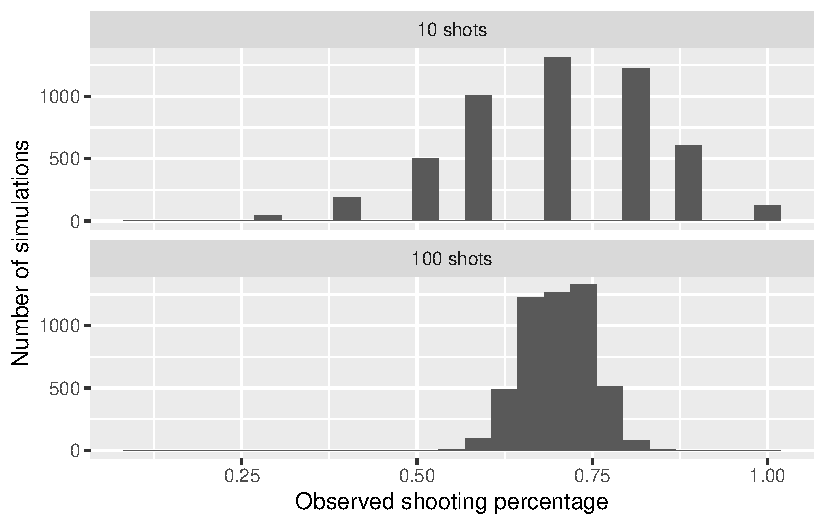
\includegraphics[keepaspectratio]{3_MeasurementError_files/figure-pdf/fig-small-large-samples-1.pdf}}

}

\caption{\label{fig-small-large-samples}Small samples vary more than
larger samples}

\end{figure}%

The 10-shot samples are much more spread out. Some look very high, and
some look very low, even though every simulated player has the same true
shooting probability.

The 100-shot samples are more tightly clustered around 0.7.

This shows why small samples can be misleading:

\begin{quote}
Small samples are noisy. They can make ordinary randomness look like a
real difference.
\end{quote}

\subsection{Coding the normal
distribution}\label{coding-the-normal-distribution}

The normal distribution gives us a way to describe variation around a
centre. It is often useful when a measurement is affected by many small
sources of random error.

Suppose repeated measurements of an object are centred around 50, with a
standard deviation of 2. We can write this as:

\[
X \sim N(50, 2)
\]

In R, we can draw the bell curve using \texttt{dnorm()}.

\begin{Shaded}
\begin{Highlighting}[]
\NormalTok{bell\_curve }\OtherTok{\textless{}{-}} \FunctionTok{tibble}\NormalTok{(}
  \AttributeTok{x =} \FunctionTok{seq}\NormalTok{(}\DecValTok{40}\NormalTok{, }\DecValTok{60}\NormalTok{, }\AttributeTok{length.out =} \DecValTok{1000}\NormalTok{),}
  \AttributeTok{density =} \FunctionTok{dnorm}\NormalTok{(x, }\AttributeTok{mean =} \DecValTok{50}\NormalTok{, }\AttributeTok{sd =} \DecValTok{2}\NormalTok{)}
\NormalTok{)}

\NormalTok{bell\_curve}
\end{Highlighting}
\end{Shaded}

\begin{verbatim}
# A tibble: 1,000 x 2
       x     density
   <dbl>       <dbl>
 1  40   0.000000743
 2  40.0 0.000000781
 3  40.0 0.000000821
 4  40.1 0.000000863
 5  40.1 0.000000907
 6  40.1 0.000000954
 7  40.1 0.00000100 
 8  40.1 0.00000105 
 9  40.2 0.00000111 
10  40.2 0.00000116 
# i 990 more rows
\end{verbatim}

The function \texttt{seq()} creates a sequence of values. Here, it
creates 1000 values from 40 to 60.

The function \texttt{dnorm()} calculates the height of the normal curve
at each value of \texttt{x}.

Here:

\begin{itemize}
\tightlist
\item
  \texttt{mean\ =\ 50} sets the centre of the curve,
\item
  \texttt{sd\ =\ 2} sets the spread of the curve.
\end{itemize}

We can plot the curve.

\begin{Shaded}
\begin{Highlighting}[]
\NormalTok{bell\_curve }\SpecialCharTok{|\textgreater{}}
  \FunctionTok{ggplot}\NormalTok{(}\FunctionTok{aes}\NormalTok{(}\AttributeTok{x =}\NormalTok{ x, }\AttributeTok{y =}\NormalTok{ density)) }\SpecialCharTok{+}
  \FunctionTok{geom\_line}\NormalTok{(}\AttributeTok{linewidth =} \DecValTok{1}\NormalTok{) }\SpecialCharTok{+}
  \FunctionTok{labs}\NormalTok{(}
    \AttributeTok{x =} \StringTok{"Observed value"}\NormalTok{,}
    \AttributeTok{y =} \StringTok{"Density"}
\NormalTok{  )}
\end{Highlighting}
\end{Shaded}

\begin{figure}[H]

\centering{

\pandocbounded{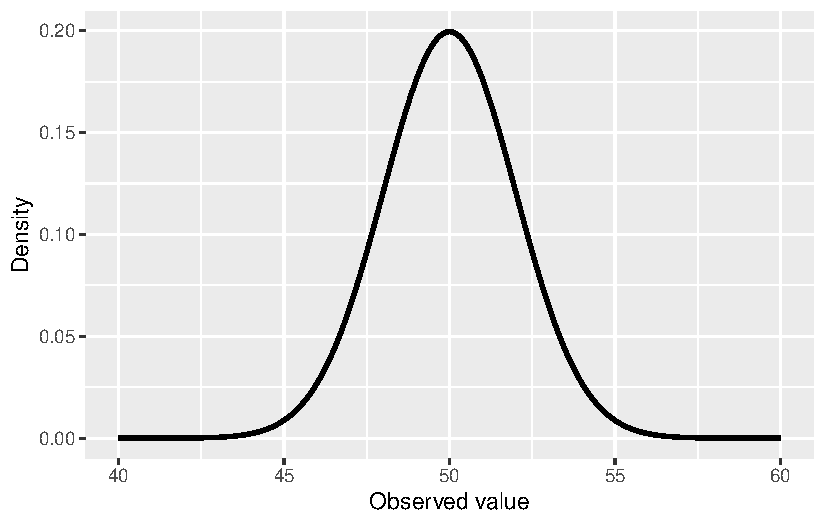
\includegraphics[keepaspectratio]{3_MeasurementError_files/figure-pdf/fig-normal-bell-curve-1.pdf}}

}

\caption{\label{fig-normal-bell-curve}A normal distribution centred at
50 with standard deviation 2}

\end{figure}%

The curve is highest near 50. Values close to 50 are more common. Values
far from 50 are less common.

Now compare two measurement processes. Both are centred around 50, but
one has smaller measurement error and the other has larger measurement
error.

\begin{Shaded}
\begin{Highlighting}[]
\NormalTok{normal\_curves }\OtherTok{\textless{}{-}} \FunctionTok{tibble}\NormalTok{(}
  \AttributeTok{x =} \FunctionTok{rep}\NormalTok{(}\FunctionTok{seq}\NormalTok{(}\DecValTok{35}\NormalTok{, }\DecValTok{65}\NormalTok{, }\AttributeTok{length.out =} \DecValTok{1000}\NormalTok{), }\DecValTok{2}\NormalTok{),}
  \AttributeTok{process =} \FunctionTok{rep}\NormalTok{(}
    \FunctionTok{c}\NormalTok{(}\StringTok{"More precise measurement"}\NormalTok{, }\StringTok{"Less precise measurement"}\NormalTok{),}
    \AttributeTok{each =} \DecValTok{1000}
\NormalTok{  )}
\NormalTok{) }\SpecialCharTok{|\textgreater{}}
  \FunctionTok{mutate}\NormalTok{(}
    \AttributeTok{density =} \FunctionTok{case\_when}\NormalTok{(}
\NormalTok{      process }\SpecialCharTok{==} \StringTok{"More precise measurement"} \SpecialCharTok{\textasciitilde{}} \FunctionTok{dnorm}\NormalTok{(x, }\AttributeTok{mean =} \DecValTok{50}\NormalTok{, }\AttributeTok{sd =} \DecValTok{2}\NormalTok{),}
\NormalTok{      process }\SpecialCharTok{==} \StringTok{"Less precise measurement"} \SpecialCharTok{\textasciitilde{}} \FunctionTok{dnorm}\NormalTok{(x, }\AttributeTok{mean =} \DecValTok{50}\NormalTok{, }\AttributeTok{sd =} \DecValTok{6}\NormalTok{)}
\NormalTok{    )}
\NormalTok{  )}

\NormalTok{normal\_curves}
\end{Highlighting}
\end{Shaded}

\begin{verbatim}
# A tibble: 2,000 x 3
       x process                   density
   <dbl> <chr>                       <dbl>
 1  35   More precise measurement 1.22e-13
 2  35.0 More precise measurement 1.36e-13
 3  35.1 More precise measurement 1.52e-13
 4  35.1 More precise measurement 1.70e-13
 5  35.1 More precise measurement 1.91e-13
 6  35.2 More precise measurement 2.13e-13
 7  35.2 More precise measurement 2.38e-13
 8  35.2 More precise measurement 2.66e-13
 9  35.2 More precise measurement 2.97e-13
10  35.3 More precise measurement 3.32e-13
# i 1,990 more rows
\end{verbatim}

The function \texttt{case\_when()} lets us calculate different values
depending on a condition. Here, we use standard deviation 2 for the more
precise process and standard deviation 6 for the less precise process.

\begin{Shaded}
\begin{Highlighting}[]
\NormalTok{normal\_curves }\SpecialCharTok{|\textgreater{}}
  \FunctionTok{ggplot}\NormalTok{(}\FunctionTok{aes}\NormalTok{(}\AttributeTok{x =}\NormalTok{ x, }\AttributeTok{y =}\NormalTok{ density, }\AttributeTok{linetype =}\NormalTok{ process)) }\SpecialCharTok{+}
  \FunctionTok{geom\_line}\NormalTok{(}\AttributeTok{linewidth =} \DecValTok{1}\NormalTok{) }\SpecialCharTok{+}
  \FunctionTok{labs}\NormalTok{(}
    \AttributeTok{x =} \StringTok{"Observed value"}\NormalTok{,}
    \AttributeTok{y =} \StringTok{"Density"}\NormalTok{,}
    \AttributeTok{linetype =} \StringTok{"Measurement process"}
\NormalTok{  )}
\end{Highlighting}
\end{Shaded}

\begin{figure}[H]

\centering{

\pandocbounded{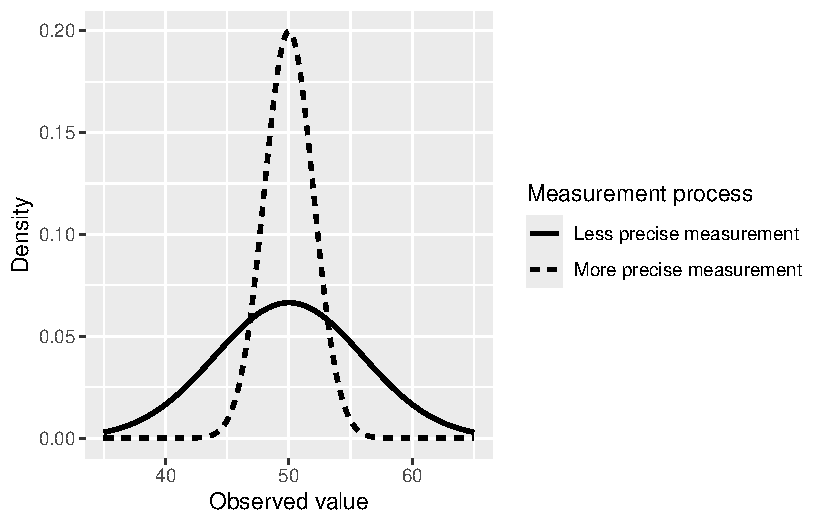
\includegraphics[keepaspectratio]{3_MeasurementError_files/figure-pdf/fig-compare-normal-curves-1.pdf}}

}

\caption{\label{fig-compare-normal-curves}Two normal distributions with
the same mean but different standard deviations}

\end{figure}%

Both curves are centred at 50. But the narrower curve is more precise:
repeated measurements cluster tightly around the centre. The wider curve
is less precise: repeated measurements are more spread out.

\section{Exercises}\label{exercises-2}

These exercises ask you to apply the ideas from this chapter to new
examples. Focus not only on the number you observe, but also on the
measurement process that produced it. In each case, ask whether the
number might contain random error, systematic error, or both.

\begin{tcolorbox}[enhanced jigsaw, arc=.35mm, bottomrule=.15mm, bottomtitle=1mm, breakable, colback=white, colbacktitle=quarto-callout-note-color!10!white, colframe=quarto-callout-note-color-frame, coltitle=black, left=2mm, leftrule=.75mm, opacityback=0, opacitybacktitle=0.6, rightrule=.15mm, title=\textcolor{quarto-callout-note-color}{\faInfo}\hspace{0.5em}{Question 1}, titlerule=0mm, toprule=.15mm, toptitle=1mm]

For each situation below, identify:

\begin{enumerate}
\def\labelenumi{\arabic{enumi}.}
\tightlist
\item
  the thing we want to know,
\item
  the number or observation we actually record,
\item
  one possible source of random error,
\item
  one possible source of systematic error.
\end{enumerate}

{\def\LTcaptype{none} % do not increment counter
\begin{longtable}[]{@{}
  >{\raggedright\arraybackslash}p{(\linewidth - 2\tabcolsep) * \real{0.5000}}
  >{\raggedright\arraybackslash}p{(\linewidth - 2\tabcolsep) * \real{0.5000}}@{}}
\toprule\noalign{}
\begin{minipage}[b]{\linewidth}\raggedright
Situation
\end{minipage} & \begin{minipage}[b]{\linewidth}\raggedright
Description
\end{minipage} \\
\midrule\noalign{}
\endhead
\bottomrule\noalign{}
\endlastfoot
A & A university course receives an average student evaluation score of
4.2 out of 5. \\
B & A fitness tracker reports that someone walked 8,740 steps in a
day. \\
C & A newspaper survey reports that 61\% of readers support a new
stadium. \\
D & A thermometer records a child's temperature as 38.1°C. \\
E & A music competition judge gives a singer a score of 82 out of
100. \\
\end{longtable}
}

\begin{quote}
\textbf{Click for Solutions}

There are several reasonable answers. One possible set is shown below.

{\def\LTcaptype{none} % do not increment counter
\begin{longtable}[]{@{}
  >{\raggedright\arraybackslash}p{(\linewidth - 8\tabcolsep) * \real{0.2000}}
  >{\raggedright\arraybackslash}p{(\linewidth - 8\tabcolsep) * \real{0.2000}}
  >{\raggedright\arraybackslash}p{(\linewidth - 8\tabcolsep) * \real{0.2000}}
  >{\raggedright\arraybackslash}p{(\linewidth - 8\tabcolsep) * \real{0.2000}}
  >{\raggedright\arraybackslash}p{(\linewidth - 8\tabcolsep) * \real{0.2000}}@{}}
\toprule\noalign{}
\begin{minipage}[b]{\linewidth}\raggedright
Situation
\end{minipage} & \begin{minipage}[b]{\linewidth}\raggedright
What we want to know
\end{minipage} & \begin{minipage}[b]{\linewidth}\raggedright
What we observe
\end{minipage} & \begin{minipage}[b]{\linewidth}\raggedright
Possible random error
\end{minipage} & \begin{minipage}[b]{\linewidth}\raggedright
Possible systematic error
\end{minipage} \\
\midrule\noalign{}
\endhead
\bottomrule\noalign{}
\endlastfoot
A & Quality of the course & Student evaluation score & Only a few
students may respond & Students with strong opinions may be more likely
to complete the survey \\
B & Actual walking activity & Step count & The tracker may misread some
arm movements & The device may consistently overcount steps for this
person's walking style \\
C & Public opinion about the stadium & Survey percentage & A different
group of readers may give a different result & Newspaper readers may not
represent the whole population \\
D & True body temperature & Thermometer reading & Slight variation due
to timing or placement & The thermometer may be poorly calibrated \\
E & Singing performance & Judge's score & The judge's mood or
performance order may affect the score & The judge may consistently
favour a particular style of music \\
\end{longtable}
}

The key idea is that the observed value is not the same as the target.
It is produced by a measurement process.
\end{quote}

\end{tcolorbox}

\begin{tcolorbox}[enhanced jigsaw, arc=.35mm, bottomrule=.15mm, bottomtitle=1mm, breakable, colback=white, colbacktitle=quarto-callout-note-color!10!white, colframe=quarto-callout-note-color-frame, coltitle=black, left=2mm, leftrule=.75mm, opacityback=0, opacitybacktitle=0.6, rightrule=.15mm, title=\textcolor{quarto-callout-note-color}{\faInfo}\hspace{0.5em}{Question 2}, titlerule=0mm, toprule=.15mm, toptitle=1mm]

Classify each source of error as mostly \textbf{random error} or mostly
\textbf{systematic error}.

\begin{enumerate}
\def\labelenumi{\alph{enumi}.}
\item
  A digital thermometer gives readings that vary slightly depending on
  exactly where it is placed.
\item
  A clock is running three minutes slow all day.
\item
  A teacher marks essays while tired, causing some small inconsistencies
  from one paper to another.
\item
  A job interview process consistently rewards applicants who attended
  the same university as the interviewer.
\item
  A survey question is worded in a way that encourages agreement.
\item
  A kitchen scale gives slightly different readings because the bowl is
  not placed in exactly the same position each time.
\end{enumerate}

\begin{quote}
\textbf{Click for Solutions}

\begin{enumerate}
\def\labelenumi{\alph{enumi}.}
\item
  Random error. The reading varies slightly from measurement to
  measurement.
\item
  Systematic error. The clock is consistently shifted in one direction.
\item
  Random error. The inconsistency varies from essay to essay.
\item
  Systematic error. The process consistently favours one group of
  applicants.
\item
  Systematic error. The question wording pushes responses in one
  direction.
\item
  Random error. Small changes in placement create small unpredictable
  changes in the reading.
\end{enumerate}

Some situations can contain both kinds of error. For example, essay
marking may include random variation between markers and systematic bias
if the rubric favours one style of writing.
\end{quote}

\end{tcolorbox}

\begin{tcolorbox}[enhanced jigsaw, arc=.35mm, bottomrule=.15mm, bottomtitle=1mm, breakable, colback=white, colbacktitle=quarto-callout-note-color!10!white, colframe=quarto-callout-note-color-frame, coltitle=black, left=2mm, leftrule=.75mm, opacityback=0, opacitybacktitle=0.6, rightrule=.15mm, title=\textcolor{quarto-callout-note-color}{\faInfo}\hspace{0.5em}{Question 3}, titlerule=0mm, toprule=.15mm, toptitle=1mm]

A person rolls a fair six-sided die three times and gets:

\[
6,\ 6,\ 6
\]

\begin{enumerate}
\def\labelenumi{\alph{enumi}.}
\item
  What is the probability of rolling three sixes in a row if the die is
  fair?
\item
  Is this enough evidence to conclude that the die is loaded?
\end{enumerate}

Now suppose the person rolls the die six times and gets:

\[
6,\ 6,\ 6,\ 6,\ 6,\ 6
\]

\begin{enumerate}
\def\labelenumi{\alph{enumi}.}
\setcounter{enumi}{2}
\item
  What is the probability of rolling six sixes in a row if the die is
  fair?
\item
  How should we interpret this result?
\end{enumerate}

\begin{quote}
\textbf{Click for Solutions}

\begin{enumerate}
\def\labelenumi{\alph{enumi}.}
\tightlist
\item
  For a fair die:
\end{enumerate}

\[
P(6,6,6)
=
\left(\frac{1}{6}\right)^3
=
\frac{1}{216}
\approx 0.00463.
\]

So the probability is about 0.46\%.

\begin{enumerate}
\def\labelenumi{\alph{enumi}.}
\setcounter{enumi}{1}
\item
  Three sixes in a row is surprising, but it still does not prove that
  the die is loaded. Rare events can happen.
\item
  For six sixes in a row:
\end{enumerate}

\[
P(6,6,6,6,6,6)
=
\left(\frac{1}{6}\right)^6
=
\frac{1}{46656}
\approx 0.0000214.
\]

That is about 0.0021\%.

\begin{enumerate}
\def\labelenumi{\alph{enumi}.}
\setcounter{enumi}{3}
\tightlist
\item
  Six sixes in a row is extremely surprising under the fair die model.
  It still does not logically prove that the die is loaded, but it gives
  strong reason to question whether the die or the rolling process is
  fair.
\end{enumerate}
\end{quote}

\end{tcolorbox}

\begin{tcolorbox}[enhanced jigsaw, arc=.35mm, bottomrule=.15mm, bottomtitle=1mm, breakable, colback=white, colbacktitle=quarto-callout-note-color!10!white, colframe=quarto-callout-note-color-frame, coltitle=black, left=2mm, leftrule=.75mm, opacityback=0, opacitybacktitle=0.6, rightrule=.15mm, title=\textcolor{quarto-callout-note-color}{\faInfo}\hspace{0.5em}{Question 4}, titlerule=0mm, toprule=.15mm, toptitle=1mm]

A new tutoring service receives three reviews in its first month. The
reviews are:

\[
5,\ 5,\ 4
\]

on a five-star scale.

\begin{enumerate}
\def\labelenumi{\alph{enumi}.}
\item
  Why might it be misleading to conclude that the tutoring service is
  excellent?
\item
  Another tutoring service has 180 reviews with an average rating of
  4.6. Why is this stronger evidence?
\item
  Does the larger number of reviews guarantee that the second service is
  better? Explain.
\end{enumerate}

\begin{quote}
\textbf{Click for Solutions}

\begin{enumerate}
\def\labelenumi{\alph{enumi}.}
\item
  Three reviews are a very small sample. They may come from unusually
  satisfied students, friends of the tutor, or people who had a
  particularly good experience.
\item
  An average based on 180 reviews is usually more stable than an average
  based on three reviews. A few unusually high or low ratings have less
  influence when there are many observations.
\item
  No.~The larger number of reviews does not guarantee that the second
  service is better. The reviews may still be biased. For example, only
  students with strong opinions may leave reviews, or the two services
  may teach different kinds of students.
\end{enumerate}
\end{quote}

\end{tcolorbox}

\begin{tcolorbox}[enhanced jigsaw, arc=.35mm, bottomrule=.15mm, bottomtitle=1mm, breakable, colback=white, colbacktitle=quarto-callout-note-color!10!white, colframe=quarto-callout-note-color-frame, coltitle=black, left=2mm, leftrule=.75mm, opacityback=0, opacitybacktitle=0.6, rightrule=.15mm, title=\textcolor{quarto-callout-note-color}{\faInfo}\hspace{0.5em}{Question 5}, titlerule=0mm, toprule=.15mm, toptitle=1mm]

Two coffee blends receive the following ratings from five reviewers.

{\def\LTcaptype{none} % do not increment counter
\begin{longtable}[]{@{}rrr@{}}
\toprule\noalign{}
Reviewer & Blend A & Blend B \\
\midrule\noalign{}
\endhead
\bottomrule\noalign{}
\endlastfoot
1 & 76 & 64 \\
2 & 78 & 72 \\
3 & 80 & 80 \\
4 & 82 & 88 \\
5 & 84 & 96 \\
\end{longtable}
}

\begin{enumerate}
\def\labelenumi{\alph{enumi}.}
\item
  Calculate the mean rating for Blend A.
\item
  Calculate the mean rating for Blend B.
\item
  Which blend has more variation in its ratings?
\item
  Explain why the two blends should not be interpreted in the same way,
  even if they have the same mean.
\end{enumerate}

\begin{quote}
\textbf{Click for Solutions}

\begin{enumerate}
\def\labelenumi{\alph{enumi}.}
\tightlist
\item
  For Blend A:
\end{enumerate}

\[
\bar{x}
=
\frac{76 + 78 + 80 + 82 + 84}{5}
=
\frac{400}{5}
=
80.
\]

\begin{enumerate}
\def\labelenumi{\alph{enumi}.}
\setcounter{enumi}{1}
\tightlist
\item
  For Blend B:
\end{enumerate}

\[
\bar{x}
=
\frac{64 + 72 + 80 + 88 + 96}{5}
=
\frac{400}{5}
=
80.
\]

\begin{enumerate}
\def\labelenumi{\alph{enumi}.}
\setcounter{enumi}{2}
\item
  Blend B has more variation. Blend A ranges from 76 to 84, while Blend
  B ranges from 64 to 96.
\item
  Blend A's ratings are tightly clustered around 80, so reviewers mostly
  agree. Blend B has the same mean, but reviewers disagree much more.
  The mean tells us the centre, but the variation tells us how stable or
  uncertain that centre is.
\end{enumerate}
\end{quote}

\end{tcolorbox}

\begin{tcolorbox}[enhanced jigsaw, arc=.35mm, bottomrule=.15mm, bottomtitle=1mm, breakable, colback=white, colbacktitle=quarto-callout-note-color!10!white, colframe=quarto-callout-note-color-frame, coltitle=black, left=2mm, leftrule=.75mm, opacityback=0, opacitybacktitle=0.6, rightrule=.15mm, title=\textcolor{quarto-callout-note-color}{\faInfo}\hspace{0.5em}{Question 6}, titlerule=0mm, toprule=.15mm, toptitle=1mm]

Two students complete five short practice tests.

Student A receives:

\[
71,\ 73,\ 72,\ 74,\ 75
\]

Student B receives:

\[
54,\ 64,\ 74,\ 84,\ 94
\]

\begin{enumerate}
\def\labelenumi{\alph{enumi}.}
\item
  Calculate the mean mark for each student.
\item
  Which student has more variation in their marks?
\item
  What might this tell us about the two students?
\end{enumerate}

\begin{quote}
\textbf{Click for Solutions}

\begin{enumerate}
\def\labelenumi{\alph{enumi}.}
\tightlist
\item
  For Student A:
\end{enumerate}

\[
\bar{x}
=
\frac{71 + 73 + 72 + 74 + 75}{5}
=
\frac{365}{5}
=
73.
\]

For Student B:

\[
\bar{x}
=
\frac{54 + 64 + 74 + 84 + 94}{5}
=
\frac{370}{5}
=
74.
\]

\begin{enumerate}
\def\labelenumi{\alph{enumi}.}
\setcounter{enumi}{1}
\item
  Student B has more variation. Their marks range from 54 to 94. Student
  A's marks range only from 71 to 75.
\item
  Student A's performance is more consistent. Student B's average is
  slightly higher, but their performance is much less stable. This could
  reflect differences in preparation, topic coverage, question type,
  confidence, or test conditions.
\end{enumerate}
\end{quote}

\end{tcolorbox}

\begin{tcolorbox}[enhanced jigsaw, arc=.35mm, bottomrule=.15mm, bottomtitle=1mm, breakable, colback=white, colbacktitle=quarto-callout-note-color!10!white, colframe=quarto-callout-note-color-frame, coltitle=black, left=2mm, leftrule=.75mm, opacityback=0, opacitybacktitle=0.6, rightrule=.15mm, title=\textcolor{quarto-callout-note-color}{\faInfo}\hspace{0.5em}{Question 7}, titlerule=0mm, toprule=.15mm, toptitle=1mm]

A machine fills bags of rice that are meant to contain 1 kg. A quality
checker weighs six bags and records:

\[
0.98,\ 1.01,\ 1.00,\ 0.99,\ 1.02,\ 1.00
\]

kilograms.

\begin{enumerate}
\def\labelenumi{\alph{enumi}.}
\item
  Are the measurements identical?
\item
  Does the variation necessarily mean the machine is broken?
\item
  What would be more worrying: this pattern, or six measurements all
  close to 1.08 kg? Explain.
\end{enumerate}

\begin{quote}
\textbf{Click for Solutions}

\begin{enumerate}
\def\labelenumi{\alph{enumi}.}
\item
  No.~The measurements vary slightly.
\item
  Not necessarily. Small variation around 1 kg may be ordinary random
  error in the filling or weighing process.
\item
  Six measurements all close to 1.08 kg would be more worrying because
  they suggest systematic error. The machine may be consistently
  overfilling the bags. The first pattern varies a little, but it is
  centred close to the target value of 1 kg.
\end{enumerate}
\end{quote}

\end{tcolorbox}

\begin{tcolorbox}[enhanced jigsaw, arc=.35mm, bottomrule=.15mm, bottomtitle=1mm, breakable, colback=white, colbacktitle=quarto-callout-note-color!10!white, colframe=quarto-callout-note-color-frame, coltitle=black, left=2mm, leftrule=.75mm, opacityback=0, opacitybacktitle=0.6, rightrule=.15mm, title=\textcolor{quarto-callout-note-color}{\faInfo}\hspace{0.5em}{Question 8}, titlerule=0mm, toprule=.15mm, toptitle=1mm]

A researcher samples balls from a box with replacement. The box contains
120 red balls and 80 blue balls.

\begin{enumerate}
\def\labelenumi{\alph{enumi}.}
\item
  What is the probability of drawing a red ball on any one draw?
\item
  If the researcher draws 10 balls and gets 8 red balls, should they
  conclude that the probability of red is 0.8?
\item
  According to the law of large numbers, what should happen to the
  observed proportion of red balls as the number of draws becomes very
  large?
\end{enumerate}

\begin{quote}
\textbf{Click for Solutions}

\begin{enumerate}
\def\labelenumi{\alph{enumi}.}
\tightlist
\item
  There are 200 balls in total, and 120 are red:
\end{enumerate}

\[
P(\text{red})
=
\frac{120}{200}
=
0.6.
\]

\begin{enumerate}
\def\labelenumi{\alph{enumi}.}
\setcounter{enumi}{1}
\item
  No.~Ten draws are a small sample. Getting 8 red balls may happen by
  chance, even though the true probability is 0.6.
\item
  As the number of draws becomes very large, the observed proportion of
  red balls should tend to get closer to the true probability, 0.6. It
  will not necessarily equal 0.6 at every point, but it should become
  more stable in the long run.
\end{enumerate}
\end{quote}

\end{tcolorbox}

\begin{tcolorbox}[enhanced jigsaw, arc=.35mm, bottomrule=.15mm, bottomtitle=1mm, breakable, colback=white, colbacktitle=quarto-callout-note-color!10!white, colframe=quarto-callout-note-color-frame, coltitle=black, left=2mm, leftrule=.75mm, opacityback=0, opacitybacktitle=0.6, rightrule=.15mm, title=\textcolor{quarto-callout-note-color}{\faInfo}\hspace{0.5em}{Question 9}, titlerule=0mm, toprule=.15mm, toptitle=1mm]

A town reports that the average daily commute time is 32 minutes.

\begin{enumerate}
\def\labelenumi{\alph{enumi}.}
\item
  Does this mean that most people commute for exactly 32 minutes?
\item
  Why would it be a mistake to use this number to predict exactly how
  long one person's commute will take tomorrow?
\item
  Give two reasons why individual commute times might vary around the
  average.
\end{enumerate}

\begin{quote}
\textbf{Click for Solutions}

\begin{enumerate}
\def\labelenumi{\alph{enumi}.}
\item
  No.~The average is a summary. Some people commute for less than 32
  minutes, and some commute for more.
\item
  An average describes a group. It does not determine an individual
  outcome. One person's commute may vary from day to day.
\item
  Possible reasons include traffic, weather, public transport delays,
  roadworks, accidents, school holidays, different departure times, or
  working from home.
\end{enumerate}

The key point is that an average gives us a centre, but it does not
describe all the variation around that centre.
\end{quote}

\end{tcolorbox}

\begin{tcolorbox}[enhanced jigsaw, arc=.35mm, bottomrule=.15mm, bottomtitle=1mm, breakable, colback=white, colbacktitle=quarto-callout-note-color!10!white, colframe=quarto-callout-note-color-frame, coltitle=black, left=2mm, leftrule=.75mm, opacityback=0, opacitybacktitle=0.6, rightrule=.15mm, title=\textcolor{quarto-callout-note-color}{\faInfo}\hspace{0.5em}{Question 10}, titlerule=0mm, toprule=.15mm, toptitle=1mm]

For each statement below, explain what is wrong or incomplete.

\begin{enumerate}
\def\labelenumi{\alph{enumi}.}
\item
  ``This course is definitely better because its student evaluation
  score is 4.3 and the other course scored 4.1.''
\item
  ``The survey says 61\%, so exactly 61\% of residents support the
  stadium.''
\item
  ``This suburb is wealthier because its average income is \$2000
  higher.''
\item
  ``The bell curve applies to all data.''
\end{enumerate}

\begin{quote}
\textbf{Click for Solutions}

\begin{enumerate}
\def\labelenumi{\alph{enumi}.}
\item
  A difference of 0.2 may be small relative to the measurement error in
  student evaluations. Response rates, student expectations, course
  difficulty, and who completed the survey may all affect the score.
\item
  A survey is produced by a measurement process. The result may depend
  on the sample, question wording, timing, and who responded. The 61\%
  is an estimate, not an exact statement about every resident.
\item
  The average alone is incomplete. We also need to know the variation,
  sample size, and distribution of incomes. A small number of
  high-income households could lift the average.
\item
  The bell curve is useful in many settings, especially where many small
  sources of variation combine, but not all data are bell-shaped. Many
  variables are skewed or have extreme outliers.
\end{enumerate}
\end{quote}

\end{tcolorbox}

\begin{tcolorbox}[enhanced jigsaw, arc=.35mm, bottomrule=.15mm, bottomtitle=1mm, breakable, colback=white, colbacktitle=quarto-callout-note-color!10!white, colframe=quarto-callout-note-color-frame, coltitle=black, left=2mm, leftrule=.75mm, opacityback=0, opacitybacktitle=0.6, rightrule=.15mm, title=\textcolor{quarto-callout-note-color}{\faInfo}\hspace{0.5em}{Question 11}, titlerule=0mm, toprule=.15mm, toptitle=1mm]

A variable is described as approximately normal:

\[
X \sim N(120, 15)
\]

\begin{enumerate}
\def\labelenumi{\alph{enumi}.}
\item
  What does 120 represent?
\item
  What does 15 represent?
\item
  In context, what would it mean if (X) represented systolic blood
  pressure?
\item
  Would a value of 122 be surprising? Would a value of 180 be more
  surprising? Explain.
\end{enumerate}

\begin{quote}
\textbf{Click for Solutions}

\begin{enumerate}
\def\labelenumi{\alph{enumi}.}
\item
  The value 120 represents the mean, or centre, of the distribution.
\item
  The value 15 represents the standard deviation, or typical spread
  around the mean.
\item
  If (X) represents systolic blood pressure, then values are centred
  around 120, with typical variation of about 15.
\item
  A value of 122 would not be surprising because it is very close to the
  mean. A value of 180 would be much more surprising because it is 60
  above the mean:
\end{enumerate}

\[
\frac{180 - 120}{15} = 4.
\]

So 180 is 4 standard deviations above the mean, which would be rare in a
normal distribution.
\end{quote}

\end{tcolorbox}

\begin{tcolorbox}[enhanced jigsaw, arc=.35mm, bottomrule=.15mm, bottomtitle=1mm, breakable, colback=white, colbacktitle=quarto-callout-note-color!10!white, colframe=quarto-callout-note-color-frame, coltitle=black, left=2mm, leftrule=.75mm, opacityback=0, opacitybacktitle=0.6, rightrule=.15mm, title=\textcolor{quarto-callout-note-color}{\faInfo}\hspace{0.5em}{Question 12}, titlerule=0mm, toprule=.15mm, toptitle=1mm]

The following table shows the number of ways to get each number of heads
in eight fair coin tosses.

{\def\LTcaptype{none} % do not increment counter
\begin{longtable}[]{@{}rr@{}}
\toprule\noalign{}
Number of heads & Number of ways \\
\midrule\noalign{}
\endhead
\bottomrule\noalign{}
\endlastfoot
0 & 1 \\
1 & 8 \\
2 & 28 \\
3 & 56 \\
4 & 70 \\
5 & 56 \\
6 & 28 \\
7 & 8 \\
8 & 1 \\
\end{longtable}
}

\begin{enumerate}
\def\labelenumi{\alph{enumi}.}
\item
  Why are 0 heads and 8 heads rare compared with 4 heads?
\item
  How does this table help explain the bell curve?
\item
  What is meant by the phrase ``the centre is crowded''?
\end{enumerate}

\begin{quote}
\textbf{Click for Solutions}

\begin{enumerate}
\def\labelenumi{\alph{enumi}.}
\tightlist
\item
  There is only one way to get 0 heads:
\end{enumerate}

\[
TTTTTTTT.
\]

There is only one way to get 8 heads:

\[
HHHHHHHH.
\]

But there are 70 different ways to get exactly 4 heads.

\begin{enumerate}
\def\labelenumi{\alph{enumi}.}
\setcounter{enumi}{1}
\item
  The table rises toward the middle and falls toward the extremes. With
  many more tosses, this same pattern becomes smoother and begins to
  resemble a bell curve.
\item
  ``The centre is crowded'' means there are many more ways to get
  outcomes near the middle than outcomes at the extremes. In
  measurement, this helps explain why small errors are often common and
  large errors are often rare.
\end{enumerate}
\end{quote}

\end{tcolorbox}

\begin{tcolorbox}[enhanced jigsaw, arc=.35mm, bottomrule=.15mm, bottomtitle=1mm, breakable, colback=white, colbacktitle=quarto-callout-note-color!10!white, colframe=quarto-callout-note-color-frame, coltitle=black, left=2mm, leftrule=.75mm, opacityback=0, opacitybacktitle=0.6, rightrule=.15mm, title=\textcolor{quarto-callout-note-color}{\faInfo}\hspace{0.5em}{Question 13}, titlerule=0mm, toprule=.15mm, toptitle=1mm]

Write a short response to the following statement:

\begin{quote}
A statistic is not just a number. It is the outcome of a process.
\end{quote}

Your response should use at least two examples not already used in your
answer above.

\begin{quote}
\textbf{Click for Solutions}

A good response should explain that statistics are produced by
measurement processes, and those processes may contain error.

For example, a fitness tracker reporting 8,740 steps is not a perfect
record of movement. It is a device-based estimate produced by sensors
and algorithms. It may miss some steps or count some non-steps.

Similarly, a student evaluation score of 4.2 is not the course quality
itself. It is produced by a survey process, and it may depend on who
responded, when the survey was completed, what students expected, and
how the questions were worded.

So before trusting a statistic, we should ask what was measured, how it
was measured, how much variation there might be, and whether systematic
bias may have entered the process.
\end{quote}

\end{tcolorbox}

\bookmarksetup{startatroot}

\chapter{Estimation}\label{estimation}

\begin{tcolorbox}[enhanced jigsaw, arc=.35mm, bottomrule=.15mm, bottomtitle=1mm, breakable, colback=white, colbacktitle=quarto-callout-note-color!10!white, colframe=quarto-callout-note-color-frame, coltitle=black, left=2mm, leftrule=.75mm, opacityback=0, opacitybacktitle=0.6, rightrule=.15mm, title=\textcolor{quarto-callout-note-color}{\faInfo}\hspace{0.5em}{Learning Objectives}, titlerule=0mm, toprule=.15mm, toptitle=1mm]

By the end of this chapter, you should be able to:

\begin{enumerate}
\def\labelenumi{\arabic{enumi}.}
\tightlist
\item
  Explain the role of estimation in moving from sample data to claims
  about a wider population.
\item
  Distinguish between populations, samples, observations, parameters,
  statistics, estimators, and estimates.
\item
  Explain the difference between observed values and random variables.
\item
  Use sample statistics, such as the mean, median, and proportion, as
  point estimates of population parameters.
\item
  Describe sampling variation and explain why different samples can
  produce different estimates.
\item
  Explain what a sampling distribution is and why it is central to
  frequentist inference.
\item
  Calculate and interpret the standard error of a sample mean.
\item
  Construct and interpret interval estimates and confidence intervals
  for a population mean.
\item
  Explain the Central Limit Theorem and describe why sample means can be
  approximately normal even when the original data are not.
\item
  Compare two means using independent and paired sample structures, and
  explain why the structure of the data matters.
\end{enumerate}

\end{tcolorbox}

\section{Introduction}\label{introduction}

The first three chapters were about preparing ourselves to think
statistically. We began with questions, because the most important
statistical mistake is often not a wrong calculation, but asking the
wrong thing. We then turned to probability, which gave us a language for
what could have happened, not just what did happen. Finally, we looked
at measurement and error, where we saw that data are not pure facts but
numbers produced by processes: surveys, instruments, definitions,
memories, records, and judgement. Some of the foundation for inference
is already here: questions, chance, variation, populations, samples, and
error.

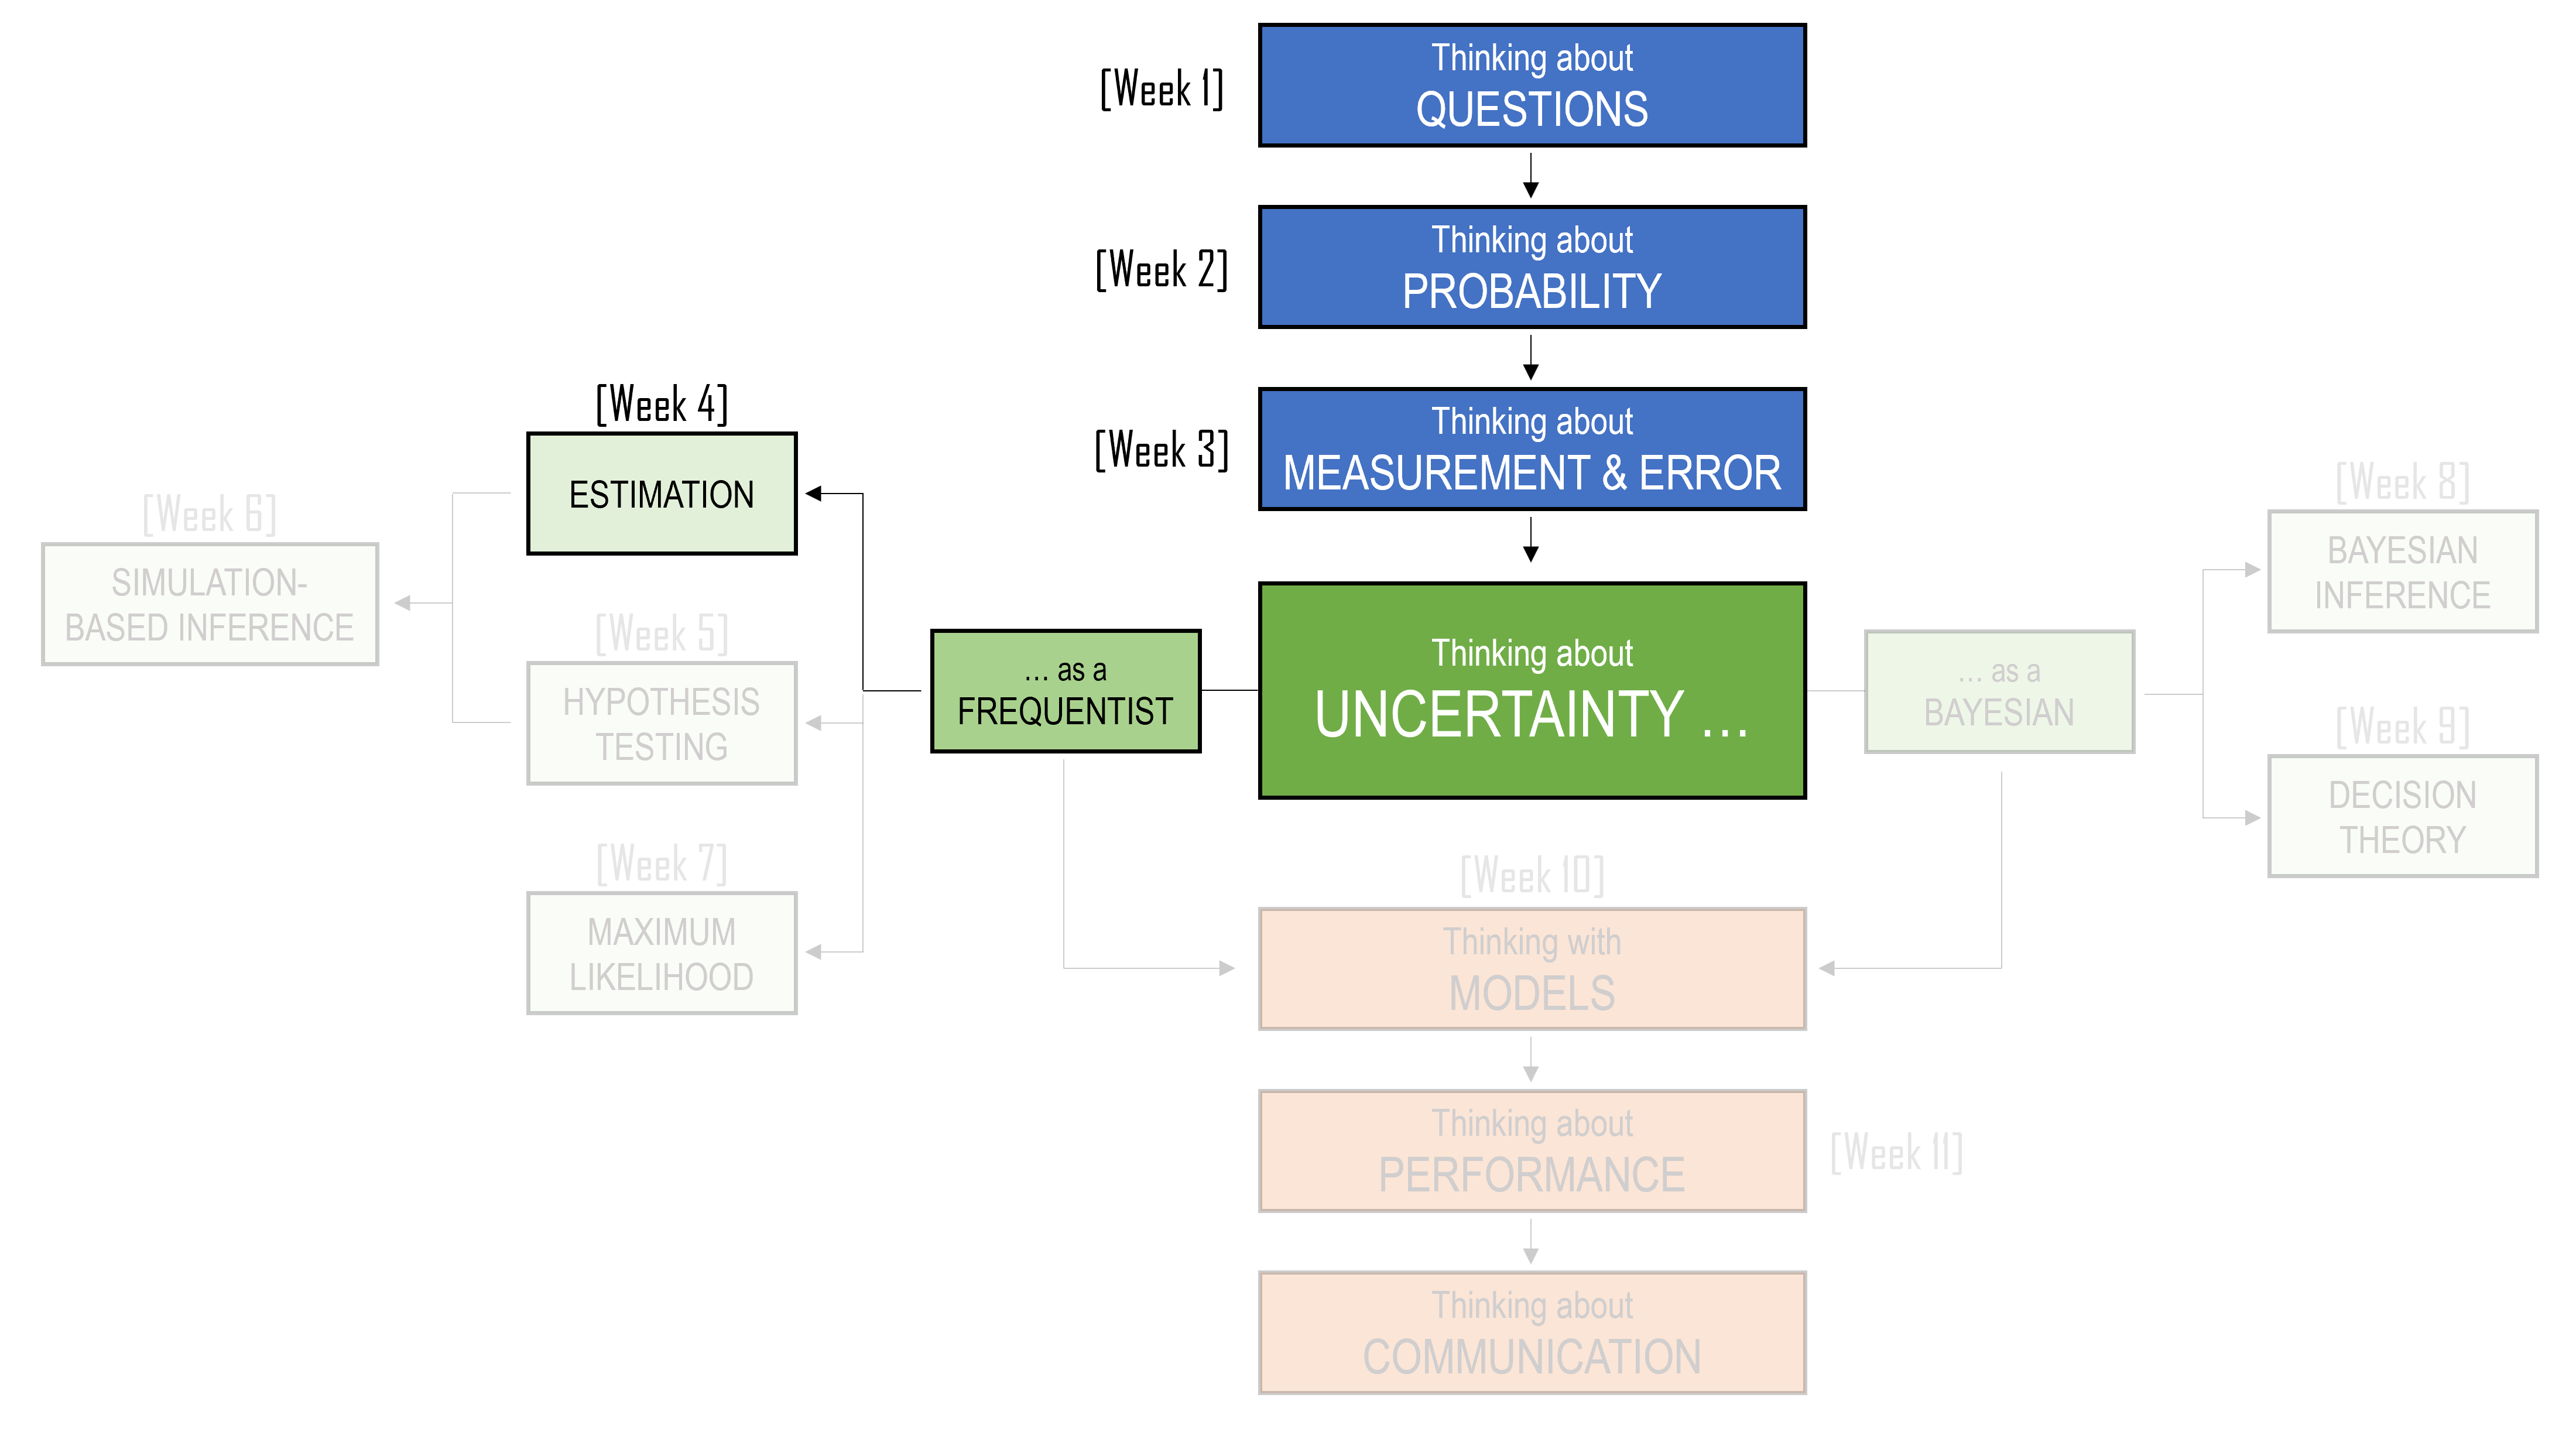
\includegraphics[width=14.67in,height=\textheight,keepaspectratio]{images/chapter4/outline.png}

As the diagram above shows, we now move into the centre of the unit:
uncertainty. Some of this may feel familiar, because the first three
chapters have already been circling around uncertainty from different
directions. But from this point on, uncertainty becomes the main object
of study. For the next six weeks, we will ask how we can learn from data
when the data could have turned out differently.

We begin with the frequentist view, where uncertainty is understood by
imagining repeated samples, repeated experiments, and repeated analyses.
Specifically, we begin this section with a discussion around estimation.

Estimation sounds simple. We want to know some quantity, so we use data
to estimate it.

\begin{itemize}
\tightlist
\item
  What is the average number of school days missed by students?
\item
  What proportion of voters support a policy?
\item
  What is the average rent near campus?
\item
  How much time do students spend studying each week?
\end{itemize}

But think back to what we have already covered in the first three
chapters:

\begin{itemize}
\tightlist
\item
  the answer depends on the question being asked
\item
  the data we observe are only one version of what could have happened
\item
  the numbers themselves are produced by imperfect measurement
  processes.
\end{itemize}

So estimation is not simply the act of calculating an average, a
proportion, or a difference. It is the act of using an imperfect number
from a particular dataset to say something careful about a wider world.
A sample average is not the population average. A poll percentage is not
the exact level of public support. A study result is not a perfect
mirror of reality. These numbers are estimates: useful, informative,
sometimes powerful, but still estimates.

The central lesson of this chapter is therefore:

\begin{quote}
One number is not the truth.
\end{quote}

This does not mean one number is useless. A single estimate can be an
excellent starting point. It can summarise a messy collection of
observations and give us something concrete to discuss. But on its own,
it is incomplete. Whenever we report an estimate, there is a question
quietly waiting behind it (and one we touched on in Chapter 3):

\begin{quote}
How wrong might this estimate be?
\end{quote}

That question will guide the rest of the chapter. We will begin with
point estimation: using a sample statistic, such as a mean or median, to
estimate an unknown population quantity. We will then look at why
estimates vary from sample to sample, even when the data are collected
carefully. This will lead us to sampling distributions, standard errors,
and confidence intervals: tools for describing the uncertainty around an
estimate.

\section{Parameters and Estimates}\label{parameters-and-estimates}

We'll use the following example to explain most of the concepts in this
chapter:

\begin{tcolorbox}[enhanced jigsaw, arc=.35mm, bottomrule=.15mm, bottomtitle=1mm, breakable, colback=white, colbacktitle=quarto-callout-note-color!10!white, colframe=quarto-callout-note-color-frame, coltitle=black, left=2mm, leftrule=.75mm, opacityback=0, opacitybacktitle=0.6, rightrule=.15mm, title=\textcolor{quarto-callout-note-color}{\faInfo}\hspace{0.5em}{Household income}, titlerule=0mm, toprule=.15mm, toptitle=1mm]

Suppose you work for the Australian Bureau of Statistics. You have been
asked to report the typical annual income of Australian households. This
sounds simple, but it immediately raises statistical questions. What
counts as a household? What counts as income? Are we interested in the
mean, the median, or the proportion of households below a particular
income level? And if we only survey a sample of households, how close
will our answer be to the truth?

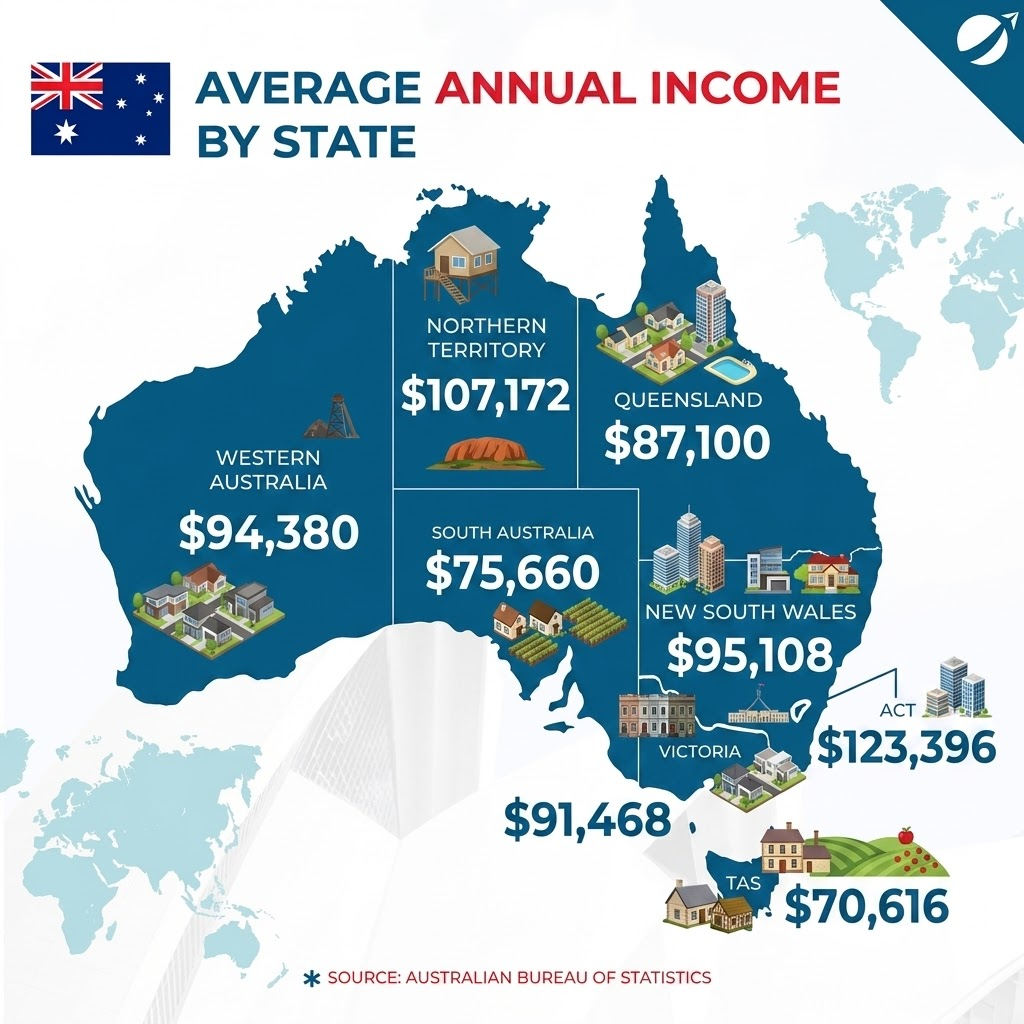
\includegraphics[width=3.41in,height=\textheight,keepaspectratio]{images/chapter4/income.jpg}

\end{tcolorbox}

Let us begin with a small illustrative dataset. Suppose we record annual
income from ten households:

\begin{table}
\fontsize{12.0pt}{14.0pt}\selectfont
\begin{tabular*}{\linewidth}{@{\extracolsep{\fill}}lr}
\toprule
Household & Annual income \\ 
\midrule\addlinespace[2.5pt]
A & \$52,000 \\ 
B & \$61,000 \\ 
C & \$68,000 \\ 
D & \$73,000 \\ 
E & \$81,000 \\ 
F & \$89,000 \\ 
G & \$97,000 \\ 
H & \$112,000 \\ 
I & \$138,000 \\ 
J & \$420,000 \\ 
\bottomrule
\end{tabular*}
\end{table}

At first glance, this looks like a simple list of numbers. But even this
small table already contains a lesson. Most households in the sample
have incomes between about \$50,000 and \$140,000. One household has an
income of \$420,000. This high value is not impossible, but it affects
some summaries more than others.

If we calculate the mean income, we get a sample mean of:

\[
\bar{x}
=
\frac{52000 + 61000 + \cdots + 420000}{10}
=
119100
\]

But does \$119,100 feel typical? Looking at the table above, seven of
the ten households have incomes below this value. The mean is not wrong,
but it has been pulled upward by the high-income household.

The median tells a different story. Since there are ten households, the
sample median is halfway between the 5th and 6th values:

\[
\text{median}
=
\frac{81000 + 89000}{2}
=
85000
\] The same data have produced two different answers:

\begin{table}
\fontsize{12.0pt}{14.0pt}\selectfont
\begin{tabular*}{\linewidth}{@{\extracolsep{\fill}}lrl}
\toprule
Summary & Value in sample & Question it answers \\ 
\midrule\addlinespace[2.5pt]
Mean & \$119,100 & If total income were shared equally, how much would each household receive? \\ 
Median & \$85,000 & What is the income of the household in the middle? \\ 
\bottomrule
\end{tabular*}
\end{table}

Both numbers are useful, but they answer different questions. The mean
is sensitive to the total amount of income in the sample. The median is
sensitive to the ordering of households. For income data, which are
often right-skewed, the median may feel closer to what we mean by a
typical household.

This brings us back to the first chapter: the question matters. There is
no single automatic answer to ``What is the typical household income?''
The answer depends on what we mean by typical.

If we care about the total amount of income spread across households,
the mean is useful. If we care about the household in the middle, the
median is more useful. If we care about economic hardship, we may
instead ask about the proportion of households below some threshold.

For example, in our sample, one household has income below \$60,000. So
the sample proportion below \$60,000 is:

\[
\hat{p}
=
\frac{1}{10}
=
0.10.
\]

That is:

\[
\hat{p} = 10\%.
\]

Now we have at least three possible quantities we might report.

\begin{table}
\fontsize{12.0pt}{14.0pt}\selectfont
\begin{tabular*}{\linewidth}{@{\extracolsep{\fill}}lrl}
\toprule
Quantity estimated from the sample & Sample value & What it tells us \\ 
\midrule\addlinespace[2.5pt]
Mean income & \$119,100 & Average income if the total were spread equally \\ 
Median income & \$85,000 & Income of the household in the middle \\ 
Proportion below \$60,000 & 10\% & Share of households below a chosen threshold \\ 
\bottomrule
\end{tabular*}
\end{table}

These are all statistics: numbers calculated from the sample. But in
estimation, the sample is not usually the final destination. We want to
use the sample to learn something about a larger population. In this
example, the population might be all Australian households. The ten
households in our table are the sample. Each household is one
observation.

\begin{tcolorbox}[enhanced jigsaw, arc=.35mm, bottomrule=.15mm, bottomtitle=1mm, breakable, colback=white, colbacktitle=quarto-callout-note-color!10!white, colframe=quarto-callout-note-color-frame, coltitle=black, left=2mm, leftrule=.75mm, opacityback=0, opacitybacktitle=0.6, rightrule=.15mm, title=\textcolor{quarto-callout-note-color}{\faInfo}\hspace{0.5em}{Terminology: population, sample, and observation}, titlerule=0mm, toprule=.15mm, toptitle=1mm]

A \textbf{population} is the full group we want to learn about.

A \textbf{sample} is the smaller group we actually observe.

An \textbf{observation} is the information recorded for one unit in the
sample.

In the household income example, the population might be all Australian
households. The sample is the households whose incomes are recorded.
Each household contributes one observation.

\end{tcolorbox}

Now we can introduce an important distinctions in statistics:

\begin{itemize}
\tightlist
\item
  A \textbf{parameter} is a numerical feature of a population.
\item
  A \textbf{statistic} is a numerical feature calculated from a sample.
\end{itemize}

For example, the true median annual income of all Australian households
is a parameter. We usually do not know it. The median income calculated
from our sample is a statistic. We do know it, once the data have been
collected. This distinction can feel small at first, but it is the
beginning of statistical inference. We use what we can calculate to
estimate what we cannot directly see.

For instance, suppose we are interested in two quantities from the
household income example:

\begin{table}
\fontsize{12.0pt}{14.0pt}\selectfont
\begin{tabular*}{\linewidth}{@{\extracolsep{\fill}}lllll}
\toprule
Target question & Population parameter & Sample statistic / estimate & Value in illustrative sample & Interpretation \\ 
\midrule\addlinespace[2.5pt]
What is the true mean annual income of all Australian households? & \(\mu\) = population mean & \(\bar{x}\) = sample mean & \(\bar{x} = 119{,}100\) & \$119,100 is our estimate of the unknown population mean. \\ 
What proportion of Australian households have annual income below \$60,000? & \(p\) = population proportion & \(\hat{p}\) = sample proportion & \(\hat{p} = 0.10\) & 10\% is our estimate of the unknown population proportion below \$60,000. \\ 
\bottomrule
\end{tabular*}
\end{table}

\begin{tcolorbox}[enhanced jigsaw, arc=.35mm, bottomrule=.15mm, bottomtitle=1mm, breakable, colback=white, colbacktitle=quarto-callout-note-color!10!white, colframe=quarto-callout-note-color-frame, coltitle=black, left=2mm, leftrule=.75mm, opacityback=0, opacitybacktitle=0.6, rightrule=.15mm, title=\textcolor{quarto-callout-note-color}{\faInfo}\hspace{0.5em}{Terminology: estimate and point estimate}, titlerule=0mm, toprule=.15mm, toptitle=1mm]

An \textbf{estimate} is a value calculated from sample data and used to
approximate an unknown parameter.

A \textbf{point estimate} is a single-number estimate.

For example, if the unknown population mean income is \(\mu\), then the
sample mean \(\bar{x}\) can be used as a point estimate of \(\mu\).

\end{tcolorbox}

To close this section, let us summarise the structure.

\begin{table}
\fontsize{12.0pt}{14.0pt}\selectfont
\begin{tabular*}{\linewidth}{@{\extracolsep{\fill}}ll}
\toprule
Step & Household income example \\ 
\midrule\addlinespace[2.5pt]
1. Define the population & All Australian households \\ 
2. Choose the parameter & Mean income, median income, or proportion below a threshold \\ 
3. Collect a sample & A surveyed set of households \\ 
4. Calculate a statistic & Sample mean, sample median, or sample proportion \\ 
5. Use the statistic as an estimate & Use the sample value to estimate the population value \\ 
\bottomrule
\end{tabular*}
\end{table}

This is the basic logic of estimation. But it leaves one large question
unanswered.

\begin{quote}
If we had chosen a different sample of households, would we have
obtained the same estimate?
\end{quote}

Almost certainly not.

The estimate depends on the sample. A different sample would give a
different sample mean, a different sample median, and a different sample
proportion. This variation from sample to sample is not a mistake. It is
the reason we need the rest of this chapter.

\section{Observed values and random
variables}\label{observed-values-and-random-variables}

In the previous section, we used the household income example to
separate the number we want to know from the number we can calculate.
The unknown population quantity is the \textbf{parameter}. The sample
quantity is the \textbf{statistic}. When we use that statistic to
approximate the parameter, it becomes an \textbf{estimate}.

But there is another distinction that is just as important, and it is
one of the reasons statistical notation can feel strange at first. The
data we have observed are fixed. They are already in the spreadsheet /
dataframe / etc. But before we collected the data, the values could have
been different. A different set of households could have been surveyed.
Their incomes could have led to a different sample mean, a different
sample median, and a different sample proportion.

Statistics needs a way to talk about both of these things:

\begin{itemize}
\tightlist
\item
  the data we actually observed;
\item
  the data we could have observed.
\end{itemize}

This is why we distinguish between \textbf{observed values} and
\textbf{random variables}.

Let us return to the household income example. In our small illustrative
sample, the ten observed incomes were:

\begin{table}
\fontsize{12.0pt}{14.0pt}\selectfont
\begin{tabular*}{\linewidth}{@{\extracolsep{\fill}}lr}
\toprule
Household & Observed income \\ 
\midrule\addlinespace[2.5pt]
A & \$52,000 \\ 
B & \$61,000 \\ 
C & \$68,000 \\ 
D & \$73,000 \\ 
E & \$81,000 \\ 
F & \$89,000 \\ 
G & \$97,000 \\ 
H & \$112,000 \\ 
I & \$138,000 \\ 
J & \$420,000 \\ 
\bottomrule
\end{tabular*}
\end{table}

Once these values are observed, they are fixed. Household A has income
\$52,000 in this dataset. Household B has income \$61,000. These numbers
are not moving around anymore.

We write the observed values using lowercase letters:

\[
x_1, x_2, \ldots, x_n
\]

For our ten households, this means:

\[
x_1 = 52000,\quad x_2 = 61000,\quad \ldots,\quad x_{10} = 420000
\]

The lowercase letter \(x\) refers to the data after they have been
observed. But before the survey was conducted, we did not know which
incomes would appear. The first household selected might have had an
income of \$52,000, or \$83,000, or \$210,000, or something else. The
second selected household also could have had many possible incomes. The
whole sample could have turned out differently.

To represent this pre-observation uncertainty, we use uppercase letters:

\[
X_1, X_2, \ldots, X_n
\]

Here, \(X_1\) represents the income of the first household before we
know what it will be. It is a \textbf{random variable}. It has not yet
landed on a value. After the sample is collected, \(X_1\) becomes
\(x_1\). The random variable has produced an observed value.

This distinction gives us two versions of the same idea.

\begin{table}
\fontsize{12.0pt}{14.0pt}\selectfont
\begin{tabular*}{\linewidth}{@{\extracolsep{\fill}}lll}
\toprule
Before data collection & After data collection & Household income example \\ 
\midrule\addlinespace[2.5pt]
\(X_1\) & \(x_1\) & Income of the first selected household, before we know it \\ 
\(X_2\) & \(x_2\) & Income of the second selected household, before we know it \\ 
\(\vdots\) & \(\vdots\) & Other possible selected households \\ 
\(X_n\) & \(x_n\) & Income of the nth selected household, before we know it \\ 
\bottomrule
\end{tabular*}
\end{table}

This matters because estimation is not only about the data in front of
us. It is about the process that produced those data. If we imagine
repeating the survey, we imagine a new set of random variables producing
a new set of observed values.

Suppose the ABS repeated the household survey tomorrow with a different
set of ten households. The sample might look like this:

\begin{table}
\fontsize{12.0pt}{14.0pt}\selectfont
\begin{tabular*}{\linewidth}{@{\extracolsep{\fill}}lr}
\toprule
Household & Observed income \\ 
\midrule\addlinespace[2.5pt]
A & \$47,000 \\ 
B & \$59,000 \\ 
C & \$64,000 \\ 
D & \$76,000 \\ 
E & \$84,000 \\ 
F & \$92,000 \\ 
G & \$105,000 \\ 
H & \$121,000 \\ 
I & \$148,000 \\ 
J & \$230,000 \\ 
\bottomrule
\end{tabular*}
\end{table}

This second sample is not wildly different from the first. It still
contains lower-income households, middle-income households, and one
relatively high-income household. But it is not identical. The largest
value is now \$230,000 rather than \$420,000.

That difference changes the summaries.

\begin{table}
\fontsize{12.0pt}{14.0pt}\selectfont
\begin{tabular*}{\linewidth}{@{\extracolsep{\fill}}lrrr}
\toprule
Sample & Mean & Median & Proportion below \$60,000 \\ 
\midrule\addlinespace[2.5pt]
First sample & \$119,100 & \$85,000 & 10\% \\ 
Second sample & \$102,600 & \$88,000 & 20\% \\ 
\bottomrule
\end{tabular*}
\end{table}

The two samples give different estimates. This is not a contradiction,
and it is not necessarily an error. It is sampling variation. This is
why we need uppercase notation. When we write the sample mean using
lowercase values,

\[
\bar{x}
=
\frac{x_1 + x_2 + \cdots + x_n}{n},
\]

we are talking about the mean of the data we actually observed. In the
first sample, this is:

\[
\bar{x} = 119100
\]

But before data collection, the sample mean itself is uncertain. It
depends on the random variables \(X_1, X_2, \ldots, X_n\). So we write
the estimator as:

\[
\bar{X}
=
\frac{X_1 + X_2 + \cdots + X_n}{n}
\]

This uppercase version, \(\bar{X}\), is a random variable. It represents
the sample mean before we know what the sample will be. Once the data
are observed, \(\bar{X}\) produces the observed estimate \(\bar{x}\).

\begin{table}
\fontsize{12.0pt}{14.0pt}\selectfont
\begin{tabular*}{\linewidth}{@{\extracolsep{\fill}}lll}
\toprule
Concept & Notation & Meaning \\ 
\midrule\addlinespace[2.5pt]
Observed values & \(x_1, x_2, \ldots, x_n\) & The household incomes actually recorded \\ 
Random variables & \(X_1, X_2, \ldots, X_n\) & The household incomes before we know what they will be \\ 
Observed sample mean & \(\bar{x}\) & The mean calculated from the observed incomes \\ 
Random sample mean & \(\bar{X}\) & The sample mean before the sample is observed \\ 
\bottomrule
\end{tabular*}
\end{table}

This distinction can feel fussy at first, but it helps us say exactly
what kind of uncertainty we are talking about.

When we write:

\[
\bar{x} = 119100,
\]

we are describing the sample we observed.

When we write:

\[
\bar{X}
=
\frac{X_1 + X_2 + \cdots + X_n}{n},
\]

we are describing the method before the data arrive. The first is an
\textbf{estimate}. The second is an \textbf{estimator}.

\section{Sampling distributions}\label{sampling-distributions}

In the previous section, we made a small but important shift. We stopped
treating the sample mean as just a number in a dataset and started
treating it as something that could have turned out differently.

For the first household income sample, the observed mean was:

\[
\bar{x} = 119{,}100
\]

But if a different set of households had been selected, the sample mean
would probably have been different. The population parameter we are
trying to estimate has not changed. The sample has changed, and
therefore the estimate has changed. This is the key idea behind a
\textbf{sampling distribution}.

\begin{tcolorbox}[enhanced jigsaw, arc=.35mm, bottomrule=.15mm, bottomtitle=1mm, breakable, colback=white, colbacktitle=quarto-callout-note-color!10!white, colframe=quarto-callout-note-color-frame, coltitle=black, left=2mm, leftrule=.75mm, opacityback=0, opacitybacktitle=0.6, rightrule=.15mm, title=\textcolor{quarto-callout-note-color}{\faInfo}\hspace{0.5em}{Terminology: sampling distribution}, titlerule=0mm, toprule=.15mm, toptitle=1mm]

A \textbf{sampling distribution} is the probability distribution of a
statistic over repeated samples.

It describes how a statistic, such as the sample mean, would vary if we
repeated the data collection process again and again.

\end{tcolorbox}

Imagine that the ABS could perform a strange experiment. Suppose it
could repeatedly draw new samples of 10 households from the same
population. For each sample, it calculates the sample mean income. The
first sample might give one mean. The second sample might give another.
The third sample might give another again.

The population has not changed. Only the sample has changed. The table
below shows the results of 8 different samples, each with 10 households.

\begin{table}
\fontsize{12.0pt}{14.0pt}\selectfont
\begin{tabular*}{\linewidth}{@{\extracolsep{\fill}}lr}
\toprule
Hypothetical sample & Sample mean income \\ 
\midrule\addlinespace[2.5pt]
Sample 1 & \$119,100 \\ 
Sample 2 & \$102,600 \\ 
Sample 3 & \$96,700 \\ 
Sample 4 & \$131,400 \\ 
Sample 5 & \$111,900 \\ 
Sample 6 & \$88,400 \\ 
Sample 7 & \$125,300 \\ 
Sample 8 & \$108,700 \\ 
\bottomrule
\end{tabular*}
\end{table}

Each row in the table is a possible result from the same sampling
process. If we took enough samples and plotted all the sample means, we
would get the sampling distribution of the sample mean.

In the app below, click on the \textbf{Take sample} button to draw a
sample of size 10 from the population. This will plot the sample mean on
the second and third panel. Repeat this \textasciitilde10 times to see
what the distribution starts to looks like. You can click the
\textbf{Take many} button, which simulates you clicking the \textbf{Take
sample} button multiple times in one go.

This repeated-sampling idea is at the centre of Frequentist statistics.
We usually do not get to take thousands of real samples. In practice,
the ABS would take one carefully designed sample and publish estimates
from that one sample. But to understand the uncertainty in those
estimates, we imagine what would happen if the sampling process were
repeated.

This imagined repetition allows us to ask questions such as:

\begin{itemize}
\tightlist
\item
  Would the sample mean usually be close to the population mean?
\item
  How far away from the population mean might it be?
\item
  Are some estimators more stable than others?
\item
  How much does the sample size matter?
\end{itemize}

A good estimator is one that tends to land close to the parameter. But
there are two different ways an estimator can fail. It can be
systematically off target. Or it can be highly unstable.

Suppose two teams are asked to estimate the average household income in
Australia.

\begin{itemize}
\item
  Team A samples only households in wealthy inner-city suburbs. Their
  estimate may be high every time. Even with a large sample, the method
  is systematically tilted upward.
\item
  Team B samples households randomly from across the country, but only
  samples five households. Their method may be fair, but their estimate
  will jump around a lot from sample to sample.
\end{itemize}

These two problems are called \textbf{bias} and \textbf{variance}.

\begin{tcolorbox}[enhanced jigsaw, arc=.35mm, bottomrule=.15mm, bottomtitle=1mm, breakable, colback=white, colbacktitle=quarto-callout-note-color!10!white, colframe=quarto-callout-note-color-frame, coltitle=black, left=2mm, leftrule=.75mm, opacityback=0, opacitybacktitle=0.6, rightrule=.15mm, title=\textcolor{quarto-callout-note-color}{\faInfo}\hspace{0.5em}{Terminology: bias and variance}, titlerule=0mm, toprule=.15mm, toptitle=1mm]

\textbf{Bias} describes whether an estimator tends to miss the parameter
systematically.

\textbf{Variance} describes how much an estimator changes from sample to
sample.

A good estimator is usually one that is centred near the truth and does
not wobble too much.

\end{tcolorbox}

In notation, if \(\hat{\theta}\) is an estimator for a parameter
\(\theta\), the bias is:

\[
\text{Bias}(\hat{\theta}) = E(\hat{\theta}) - \theta
\]

The variance of the estimator is:

\[
\text{Var}(\hat{\theta})
\]

The bias tells us whether the estimator is centred in the wrong place.
The variance tells us how spread out the sampling distribution is.

The household income example helps make this concrete. If we sample only
wealthy suburbs, the sampling distribution of the sample mean may be
centred above the true national mean. That is bias. If we take very
small random samples, the sampling distribution may be centred near the
true national mean but spread very widely. That is high variance.

\pandocbounded{
\includegraphics[keepaspectratio]{4_Estimation_files/figure-pdf/unnamed-chunk-16-1.pdf}}

The dashed line represents the true population mean. In a real study, we
would not know where this line is. But the picture is useful because it
shows what we want from an estimator. We want the sampling distribution
to be centred near the parameter. We also want it to be narrow. Centred
means low bias. Narrow means low variance.

This is why sampling design matters so much. A very large biased sample
can still be misleading. Sampling only households from a wealthy suburb
may produce a very precise estimate of the wrong thing. More data do not
automatically fix a bad design.

It is also why sample size matters. If the sampling is sound, larger
samples usually make estimates more stable. A sample of 10 households
may produce an estimate that moves around a great deal. A sample of
1,000 households will usually produce a sample mean that varies less
from sample to sample.

To see the basic idea, imagine repeatedly sampling from the same
population of household incomes, but changing the sample size.

\pandocbounded{
\includegraphics[keepaspectratio]{4_Estimation_files/figure-pdf/unnamed-chunk-17-1.pdf}}

The individual household incomes are still uneven and right-skewed. But
the sample mean becomes more stable as the sample size grows. This is
one of the reasons averages are so useful. They smooth out some of the
disorder in individual observations.

But notice the wording: \textbf{some} of the disorder. Averages do not
remove all uncertainty. They reduce sampling variation, especially when
the sample size is large and the sampling process is well designed. They
do not automatically remove bias, measurement problems, or poor
definitions.

\begin{tcolorbox}[enhanced jigsaw, arc=.35mm, bottomrule=.15mm, bottomtitle=1mm, breakable, colback=white, colbacktitle=quarto-callout-warning-color!10!white, colframe=quarto-callout-warning-color-frame, coltitle=black, left=2mm, leftrule=.75mm, opacityback=0, opacitybacktitle=0.6, rightrule=.15mm, title=\textcolor{quarto-callout-warning-color}{\faExclamationTriangle}\hspace{0.5em}{Larger samples do not fix every problem}, titlerule=0mm, toprule=.15mm, toptitle=1mm]

A larger random sample usually reduces sampling variation. But a larger
sample does not automatically remove bias. If the sampling process
misses some kinds of households, or if income is measured
inconsistently, a large sample can still produce a misleading estimate.

\end{tcolorbox}

The sampling distribution is therefore not just a technical idea. It is
the picture behind uncertainty.

When we report a point estimate, such as:

\[
\bar{x} = 119{,}100,
\]

we are reporting one realised value from a process that could have
produced other values.

The natural next question is:

\begin{quote}
How much would this estimate tend to vary from sample to sample?
\end{quote}

\section{Standard error: the wobble of an
estimate}\label{standard-error-the-wobble-of-an-estimate}

At the end of the previous section, we reached a new question. If a
statistic changes from sample to sample, then how much does it change?

This is not a small detail. It is the difference between an estimate
that is useful and an estimate that is floating in space with no sense
of reliability. Saying that the sample mean household income is
\(\$119{,}100\) gives us a number. But it does not yet tell us how much
trust to place in that number.

To do that, we need to measure the \textbf{wobble} of the estimate.

In the household income example, there are two different kinds of wobble
we might care about.

\begin{itemize}
\tightlist
\item
  First, individual households differ from one another. Some households
  have lower incomes, some have middle incomes, and a few have much
  higher incomes. This is variation in the data.
\item
  Second, sample means differ from one sample to another. One sample
  might produce a mean of \(\$119{,}100\). Another might produce
  \(\$102{,}600\). Another might produce something else. This is
  variation in the estimate.
\end{itemize}

These are related, but they are not the same thing.

\begin{tcolorbox}[enhanced jigsaw, arc=.35mm, bottomrule=.15mm, bottomtitle=1mm, breakable, colback=white, colbacktitle=quarto-callout-important-color!10!white, colframe=quarto-callout-important-color-frame, coltitle=black, left=2mm, leftrule=.75mm, opacityback=0, opacitybacktitle=0.6, rightrule=.15mm, title=\textcolor{quarto-callout-important-color}{\faExclamation}\hspace{0.5em}{Do not confuse these two quantities}, titlerule=0mm, toprule=.15mm, toptitle=1mm]

The \textbf{standard deviation} describes how much individual
observations vary.

The \textbf{standard error} describes how much an estimate varies from
sample to sample.

In the household income example, the standard deviation is about
variation among household incomes. The standard error is about variation
among sample mean incomes.

\end{tcolorbox}

Let us return to the small household income sample, which had a sample
mean of:

\[
\bar{x} = 119{,}100
\]

The sample standard deviation is:

\[
s
=
\sqrt{
\frac{1}{n-1}
\sum_{i=1}^{n}
(x_i - \bar{x})^2
}
=108{,}735
\]

The sample standard deviation is large because the incomes themselves
are spread out, especially because of the high-income household.

For a sample mean, the standard error has a particularly important form:

\[
SE(\bar{X}) = \frac{\sigma}{\sqrt{n}}
\]

Here, \(\sigma\) is the population standard deviation and \(n\) is the
sample size. This formula says two important things.

\begin{itemize}
\tightlist
\item
  First, if individual households are highly variable, then sample means
  will also be more variable. Income is much harder to estimate
  precisely when households differ greatly from one another.
\item
  Second, larger samples produce more stable sample means. The sample
  size appears under a square root, so increasing \(n\) reduces the
  standard error.
\end{itemize}

But there is a catch. In real life, we usually do not know \(\sigma\),
the population standard deviation. If we knew the population standard
deviation, we might already know a lot about the population. Instead, we
estimate \(\sigma\) using \(s\), the sample standard deviation.

So in practice we often use:

\[
se(\bar{x}) = \frac{s}{\sqrt{n}}
\]

For the household income sample:

\[
se(\bar{x})
=
\frac{s}{\sqrt{n}}
=
\frac{108735}{\sqrt{10}}
=
34387
\]

So the estimated standard error of the sample mean is about \$34,386.

This number is not saying that household incomes are typically about
\$34,386 away from the mean. That would be a statement about the
standard deviation. Instead, it says that the sample mean itself would
tend to vary by roughly this amount from sample to sample, under the
assumptions we are using.

This is why the standard error is useful with estimation. It gives a
scale for uncertainty. Without it, a point estimate is lonely. With it,
we begin to see how precise, or imprecise, the estimate might be. A
useful reporting style is:

\[
\text{estimate} \pm \text{standard error}
\]

For our sample:

\[
119{,}100 \pm 34{,}387
\]

This is already more informative than reporting \(\$119{,}100\) alone.
It tells the reader that the estimate is not especially precise. With
only ten households and one very high-income household, the sample mean
is quite wobbly.

Now let us look at why sample size matters. Suppose the household
incomes in the wider population are highly variable. That variability is
a fact about the population. We cannot make Australian households less
economically diverse by collecting more data. But we can make our
estimate of the mean more stable by collecting a larger sample.

The formula tells us why:

\[
se(\bar{x}) = \frac{s}{\sqrt{n}}
\]

As \(n\) increases, the denominator gets larger, so the standard error
gets smaller.

\begin{table}
\fontsize{12.0pt}{14.0pt}\selectfont
\begin{tabular*}{\linewidth}{@{\extracolsep{\fill}}rr}
\toprule
Sample size & Estimated standard error \\ 
\midrule\addlinespace[2.5pt]
10 & \$34,385 \\ 
25 & \$21,747 \\ 
100 & \$10,873 \\ 
400 & \$5,437 \\ 
1600 & \$2,718 \\ 
\bottomrule
\end{tabular*}
\end{table}

The standard error falls as the sample size grows. But it does not fall
in a straight line. Because the sample size is under a square root,
reducing the standard error substantially requires a much larger sample.
To halve the standard error, we need about four times as much data.

For example:

\[
\sqrt{4n} = 2\sqrt{n}
\]

So:

\[
\frac{s}{\sqrt{4n}}
=
\frac{s}{2\sqrt{n}}
=
\frac{1}{2}\frac{s}{\sqrt{n}}
\]

This is one of the quiet realities of survey work. Precision is
expensive. Asking ten households is easy but unstable. Asking one
thousand households is much better, but it takes planning, money, time,
and careful design.

\pandocbounded{
\includegraphics[keepaspectratio]{4_Estimation_files/figure-pdf/unnamed-chunk-19-1.pdf}}

The curve drops quickly at first, then flattens out. This is the
mathematical version of a familiar practical problem: early improvements
can be large, but each additional gain in precision costs more and more
data.

\begin{tcolorbox}[enhanced jigsaw, arc=.35mm, bottomrule=.15mm, bottomtitle=1mm, breakable, colback=white, colbacktitle=quarto-callout-important-color!10!white, colframe=quarto-callout-important-color-frame, coltitle=black, left=2mm, leftrule=.75mm, opacityback=0, opacitybacktitle=0.6, rightrule=.15mm, title=\textcolor{quarto-callout-important-color}{\faExclamation}\hspace{0.5em}{Precision has a cost}, titlerule=0mm, toprule=.15mm, toptitle=1mm]

Increasing the sample size reduces the standard error, but with
diminishing returns. To halve the standard error, we generally need
about four times the sample size.

\end{tcolorbox}

The standard error also helps us compare two estimates that look similar
on the surface.

Suppose one household survey reports an estimated average income of
\(\$119{,}100\), with a standard error of \(\$38{,}323\). Another much
larger survey reports an estimated average income of \(\$105{,}000\),
with a standard error of \(\$2{,}000\).

The first estimate is higher, but much less precise. The second estimate
is lower, but much more stable.

\begin{table}
\fontsize{12.0pt}{14.0pt}\selectfont
\begin{tabular*}{\linewidth}{@{\extracolsep{\fill}}lrrl}
\toprule
Survey & Estimate & Standard error & Interpretation \\ 
\midrule\addlinespace[2.5pt]
Small survey & \$119,100 & \$38,323 & Higher estimate, but very uncertain \\ 
Large survey & \$105,000 & \$2,000 & Lower estimate, but much more precise \\ 
\bottomrule
\end{tabular*}
\end{table}

A point estimate alone might tempt us to focus on \(\$119{,}100\),
because it is larger. But the standard error tells us that this number
is not very stable. The large survey's estimate may be more useful, even
though it is less dramatic.

A statistical estimate should not be judged only by where it lands. It
should also be judged by how much it wobbles. The standard error gives
us that wobble in a single number. But often we want to communicate
uncertainty as a range rather than as a separate quantity. That takes us
to \textbf{interval estimation}.

\section{Interval estimation}\label{interval-estimation}

A standard error gives us one useful number: the typical wobble of an
estimate. For the household income sample, we estimated the mean annual
income as:

\[
\bar{x} = 119{,}100
\]

The estimated standard error was about:

\[
se(\bar{x}) = 34{,}385
\]

So we could report:

\[
119{,}100 \pm 34{,}385
\]

This is better than reporting the point estimate alone, because it gives
the reader some sense of uncertainty. But it still requires a little
mental work. The reader has to remember what ``plus or minus one
standard error'' means, and they still have to translate it into a
range.

A more direct way to communicate uncertainty is to report an
\textbf{interval estimate}.

Instead of saying:

\begin{quote}
Our estimate is \$119,100
\end{quote}

we say something like:

\begin{quote}
Our estimate is \$119,100, with a plausible range from about \$50,330 to
\$187,870
\end{quote}

The exact range depends on the method we use, but the general idea is
simple:

\[
\text{interval estimate}
=
\left(
\text{estimate} - \text{error},
\text{estimate} + \text{error}
\right).
\]

Or, in a more familiar shorthand:

\[
\text{estimate} \pm \text{error}
\]

\begin{tcolorbox}[enhanced jigsaw, arc=.35mm, bottomrule=.15mm, bottomtitle=1mm, breakable, colback=white, colbacktitle=quarto-callout-note-color!10!white, colframe=quarto-callout-note-color-frame, coltitle=black, left=2mm, leftrule=.75mm, opacityback=0, opacitybacktitle=0.6, rightrule=.15mm, title=\textcolor{quarto-callout-note-color}{\faInfo}\hspace{0.5em}{Terminology: interval estimate}, titlerule=0mm, toprule=.15mm, toptitle=1mm]

An \textbf{interval estimate} gives a range of plausible values for a
parameter.

A \textbf{point estimate} gives one number.

An \textbf{interval estimate} gives a lower value and an upper value.

\end{tcolorbox}

For the household income example, the point estimate is the sample mean:

\[
\bar{x} = 119{,}100
\]

A rough interval estimate can be formed by going two standard errors
below and above the estimate:

\[
\bar{x} \pm 2 \times se(\bar{x})
\]

Substituting the values from our sample:

\[
119{,}100 \pm 2(34{,}385)
=
119{,}100 \pm 68{,}770
\]

This gives:

\[
(50{,}330,\ 187{,}870)
\]

So instead of presenting only one number, we can say:

\begin{quote}
Based on this sample, the estimated mean annual household income is
\$119,100, with a rough plausible range from about \$50,330 to \$187,870
\end{quote}

That is a very wide range. But that is the point. With only ten
households, and with one very high-income household in the sample, we
should not pretend to have a precise estimate.

The interval does not make the result weaker. It makes the uncertainty
visible.

\pandocbounded{
\includegraphics[keepaspectratio]{4_Estimation_files/figure-pdf/unnamed-chunk-21-1.pdf}}

The dot is the point estimate. The line is the interval estimate. The
dot tells us where our sample landed. The line reminds us that the
population value might plausibly be somewhere else. This is especially
important when different samples produce different estimates. Suppose
two small household income surveys produce the following results:

\begin{table}
\fontsize{12.0pt}{14.0pt}\selectfont
\begin{tabular*}{\linewidth}{@{\extracolsep{\fill}}lrrrr}
\toprule
Survey & Estimate & Standard error & Lower & Upper \\ 
\midrule\addlinespace[2.5pt]
Survey A & \$119,100 & \$34,385 & \$50,330 & \$187,870 \\ 
Survey B & \$102,600 & \$28,000 & \$46,600 & \$158,600 \\ 
\bottomrule
\end{tabular*}
\end{table}

The point estimates are different:

\[
119{,}100
\quad \text{and} \quad
102{,}600
\]

If we focused only on the point estimates, we might be tempted to tell a
story about the difference. Perhaps income has changed. Perhaps one
survey found a richer group of households. Perhaps something interesting
is going on. But once we include the uncertainty, the story becomes more
cautious. Both intervals are wide. The difference between the two point
estimates may not be very surprising, because small samples can wobble
quite a lot.

\pandocbounded{
\includegraphics[keepaspectratio]{4_Estimation_files/figure-pdf/unnamed-chunk-23-1.pdf}}

This is one of the habits we want to develop in statistical thinking:

\begin{quote}
Do not compare estimates without also comparing their uncertainty.
\end{quote}

A difference between two point estimates can look meaningful simply
because we have hidden the wobble. Once the uncertainty is visible, the
difference may look less dramatic.

\begin{tcolorbox}[enhanced jigsaw, arc=.35mm, bottomrule=.15mm, bottomtitle=1mm, breakable, colback=white, colbacktitle=quarto-callout-important-color!10!white, colframe=quarto-callout-important-color-frame, coltitle=black, left=2mm, leftrule=.75mm, opacityback=0, opacitybacktitle=0.6, rightrule=.15mm, title=\textcolor{quarto-callout-important-color}{\faExclamation}\hspace{0.5em}{Point estimates can overstate certainty}, titlerule=0mm, toprule=.15mm, toptitle=1mm]

A point estimate is useful, but it can make a result look more precise
than it really is. An interval estimate reminds us that the statistic
came from one sample, and another sample could have produced another
value.

\end{tcolorbox}

So far, we have used a rough rule:

\[
\text{estimate} \pm 2 \times \text{standard error}
\]

This is a useful first approximation, and it often gives the right
intuition. But it is not the full story. In formal Frequentist
statistical inference, the most common interval estimate is the
\textbf{confidence interval}.

A confidence interval has the same broad shape:

\[
\text{estimate} \pm \text{multiplier} \times \text{standard error}.
\]

The multiplier depends on the confidence level, the sample size, and the
probability model being used. For a 95\% confidence interval, the
multiplier is often close to 2, but not always exactly 2.

For example, when estimating a population mean and using the sample
standard deviation, the interval often takes the form:

\[
\bar{x}
\pm
t_{n-1,0.975}
\frac{s}{\sqrt{n}}.
\]

This looks more complicated, but the structure is the same:

\[
\text{estimate}
\pm
\text{multiplier}
\times
\text{standard error}.
\]

The point estimate tells us where the interval is centred. The standard
error tells us the scale of the uncertainty. The multiplier tells us how
wide the interval should be for the confidence level we want.

\begin{tcolorbox}[enhanced jigsaw, arc=.35mm, bottomrule=.15mm, bottomtitle=1mm, breakable, colback=white, colbacktitle=quarto-callout-note-color!10!white, colframe=quarto-callout-note-color-frame, coltitle=black, left=2mm, leftrule=.75mm, opacityback=0, opacitybacktitle=0.6, rightrule=.15mm, title=\textcolor{quarto-callout-note-color}{\faInfo}\hspace{0.5em}{The general shape of many intervals}, titlerule=0mm, toprule=.15mm, toptitle=1mm]

Many statistical intervals have the form:

\[
\text{estimate}
\pm
\text{multiplier}
\times
\text{standard error}.
\]

The details change from problem to problem, but the basic logic is the
same.

\end{tcolorbox}

For our small household income sample, the rough interval using \(2\) as
the multiplier was:

\[
119{,}100 \pm 2(34{,}385)
\]

A formal 95\% confidence interval would use a multiplier from the
\(t\)-distribution rather than exactly 2. Since the sample size is
\(n=10\), the relevant degrees of freedom are:

\[
n - 1 = 9.
\]

The multiplier is approximately:

\[
t_{9,0.975} = 2.262.
\]

So the formal interval is:

\[
119{,}100 \pm 2.262(34{,}385)
\]

That is:

\[
119{,}100 \pm 77{,}784
\]

which gives:

\[
(41{,}316,\ 196{,}884)
\]

The formal interval is slightly wider than the rough two-standard-error
interval. This is because the sample size is small, and the
\(t\)-distribution allows for the extra uncertainty created by
estimating the standard deviation from the same small sample.

\begin{table}
\fontsize{12.0pt}{14.0pt}\selectfont
\begin{tabular*}{\linewidth}{@{\extracolsep{\fill}}lrrr}
\toprule
Method & Multiplier & Lower & Upper \\ 
\midrule\addlinespace[2.5pt]
Rough interval & 2.000 & \$50,330 & \$187,870 \\ 
95\% t confidence interval & 2.262 & \$41,316 & \$196,884 \\ 
\bottomrule
\end{tabular*}
\end{table}

This table shows that the rough interval and the formal confidence
interval are built from the same ingredients. The difference is the
multiplier.

The rough interval uses \(2\), which is easy to remember.

The formal interval uses \(t_{9,0.975}\), which is more appropriate for
a sample mean with a small sample size.

In practice, we usually let software calculate the interval. But it is
important to understand the structure, because the software is not doing
magic. It is taking an estimate, measuring its wobble, choosing a
multiplier, and turning the result into a range.

That raises the next question:

\begin{quote}
What exactly does the ``95\%'' in a 95\% confidence interval mean?
\end{quote}

\section{Confidence intervals}\label{confidence-intervals}

The previous section ended with a question that sounds innocent:

\begin{quote}
What does the ``95\%'' in a 95\% confidence interval mean?
\end{quote}

This is one of the most misunderstood ideas in statistics. The phrase
``95\% confidence'' sounds as though it should mean something simple,
like:

\begin{quote}
There is a 95\% chance that the true value is inside this interval.
\end{quote}

That sentence is tempting. It is also not quite right, at least not from
the Frequentist point of view. To see why, return to the household
income example. Our formal 95\% confidence interval for the population
mean was approximately:

\[
(41{,}316,\ 196{,}884)
\]

This interval was calculated from the sample. Once we have observed the
data, the interval is fixed. It starts at \(41{,}316\) and ends at
\(196{,}884\). The true population mean, \(\mu\), is also fixed. We may
not know it, but it is not moving around.

So after the interval has been calculated, there are only two
possibilities:

\begin{itemize}
\tightlist
\item
  the interval contains \(\mu\);
\item
  or the interval does not contain \(\mu\).
\end{itemize}

There is no longer any randomness in this particular interval. The
randomness was in the sampling process that produced it.

So what does the 95\% refer to? It refers to the long-run behaviour of
the method. Imagine repeating the household income survey many times.
Each time, we take a new sample, calculate a new sample mean, calculate
a new standard error, and construct a new confidence interval using the
same procedure.

Some of those intervals will contain the true population mean. Some will
miss it. A 95\% confidence interval procedure is designed so that, in
the long run, about 95\% of the intervals produced by that method will
contain the true parameter. The confidence is in the \textbf{procedure},
not in the one interval after it has been calculated.

\begin{tcolorbox}[enhanced jigsaw, arc=.35mm, bottomrule=.15mm, bottomtitle=1mm, breakable, colback=white, colbacktitle=quarto-callout-note-color!10!white, colframe=quarto-callout-note-color-frame, coltitle=black, left=2mm, leftrule=.75mm, opacityback=0, opacitybacktitle=0.6, rightrule=.15mm, title=\textcolor{quarto-callout-note-color}{\faInfo}\hspace{0.5em}{Terminology: confidence interval}, titlerule=0mm, toprule=.15mm, toptitle=1mm]

A \textbf{confidence interval} is an interval estimate constructed by a
method that has a specified long-run success rate.

A 95\% confidence interval procedure is one that, under the assumptions
of the model, produces intervals that contain the true parameter in 95\%
of repeated samples.

\end{tcolorbox}

This is a bit of a mouthful. But the idea is easier to see than to say.
Suppose the true average household income were known to be
\(\mu = 100{,}000\). In real life, we would not know this value. But for
the purpose of illustration, imagine that we do. Now suppose we
repeatedly take samples and construct 95\% confidence intervals. Each
interval is different, because each sample is different.

\pandocbounded{
\includegraphics[keepaspectratio]{4_Estimation_files/figure-pdf/unnamed-chunk-25-1.pdf}}

Each horizontal line is a confidence interval from a different sample.
The dot marks the sample mean for that sample. The vertical dashed line
marks the true population mean in this simulation.

Most intervals cross the dashed line. A few do not. That is what the
confidence level means. It is not a promise that any one interval is
correct. It is a statement about the long-run performance of the method.

This repeated-sampling interpretation may feel awkward, but it is the
core of Frequentist thinking. We usually observe one sample, but we
evaluate our methods by imagining what would happen if the sampling
process were repeated again and again.

In practice, when we communicate results, we often use more intuitive
language. We might say:

\begin{quote}
The 95\% confidence interval gives a range of plausible values for the
population mean, given the data and the assumptions.
\end{quote}

This is not the formal definition, but it is often a useful way to
explain what the interval is doing. It reminds the reader not to focus
only on the point estimate.

For the household income example, we might report:

\begin{quote}
In this small sample, the mean annual household income was estimated to
be \$119,100. A 95\% confidence interval for the population mean is
approximately \$41,316 to \$196,884.
\end{quote}

This sentence does three useful things. It gives the point estimate. It
gives the uncertainty. And it avoids pretending that the sample mean is
the exact population mean.

But we should still be careful. A confidence interval only accounts for
the uncertainty described by the model. It does not automatically fix
problems in the data.

If the households were sampled only from wealthy suburbs, the confidence
interval might be narrow but centred in the wrong place. If income was
measured inconsistently, the interval would not magically correct the
measurement problem. If the sample missed some kinds of households
altogether, the interval would not know that.

\begin{tcolorbox}[enhanced jigsaw, arc=.35mm, bottomrule=.15mm, bottomtitle=1mm, breakable, colback=white, colbacktitle=quarto-callout-warning-color!10!white, colframe=quarto-callout-warning-color-frame, coltitle=black, left=2mm, leftrule=.75mm, opacityback=0, opacitybacktitle=0.6, rightrule=.15mm, title=\textcolor{quarto-callout-warning-color}{\faExclamationTriangle}\hspace{0.5em}{Confidence intervals do not fix bad data}, titlerule=0mm, toprule=.15mm, toptitle=1mm]

A confidence interval describes uncertainty from sampling variation,
under a set of assumptions.

It does not automatically correct bias, poor measurement, non-response,
or a badly chosen sample.

\end{tcolorbox}

This is why confidence intervals should be reported with context. The
interval tells us about uncertainty in the estimate, but the quality of
the estimate still depends on the quality of the data collection.

The formula we used for the household income example was:

\[
\bar{x}
\pm
t_{n-1,0.975}
\frac{s}{\sqrt{n}}.
\]

This is a confidence interval for a population mean. It has three
ingredients.

\begin{table}
\fontsize{12.0pt}{14.0pt}\selectfont
\begin{tabular*}{\linewidth}{@{\extracolsep{\fill}}lll}
\toprule
Ingredient & Symbol & Role in the interval \\ 
\midrule\addlinespace[2.5pt]
Point estimate & \(\bar{x}\) & Centres the interval \\ 
Standard error & \(\frac{s}{\sqrt{n}}\) & Measures the wobble of the estimate \\ 
Multiplier & \(t_{n-1,0.975}\) & Controls how wide the interval is \\ 
\bottomrule
\end{tabular*}
\end{table}

The point estimate tells us where the interval is centred. The standard
error tells us how much the estimate tends to wobble. The multiplier
tells us how much wobble to allow for.

For our sample:

\[
\bar{x} = 119{,}100,
\]

\[
se(\bar{x}) = 34{,}385,
\]

and, because \(n = 10\),

\[
t_{9,0.975} \approx 2.262.
\]

So:

\[
119{,}100
\pm
2.262(34{,}385)
=
119{,}100
\pm
77{,}784.
\]

This gives:

\[
(41{,}316,\ 196{,}884).
\]

The interval is wide. But that is not a failure of the method. It is an
honest reflection of the data: the sample is small, and the incomes vary
a lot.

A wider interval says:

\begin{quote}
We have less precision.
\end{quote}

A narrower interval says:

\begin{quote}
We have more precision.
\end{quote}

But a narrow interval is not automatically better if it is built from
biased or poor-quality data. Precision and truth are not the same thing.

\begin{tcolorbox}[enhanced jigsaw, arc=.35mm, bottomrule=.15mm, bottomtitle=1mm, breakable, colback=white, colbacktitle=quarto-callout-note-color!10!white, colframe=quarto-callout-note-color-frame, coltitle=black, left=2mm, leftrule=.75mm, opacityback=0, opacitybacktitle=0.6, rightrule=.15mm, title=\textcolor{quarto-callout-note-color}{\faInfo}\hspace{0.5em}{Precision and accuracy}, titlerule=0mm, toprule=.15mm, toptitle=1mm]

A \textbf{precise} estimate has little sampling variation, so its
confidence interval is narrow.

An \textbf{accurate} estimate is close to the true parameter.

A large, biased sample can produce a precise estimate of the wrong
quantity.

\end{tcolorbox}

This distinction matters in official statistics. A national income
estimate should not merely be precise. It should be meaningful,
well-defined, and based on a sample that represents the population of
interest.

So the question is not only:

\begin{quote}
How wide is the interval?
\end{quote}

It is also:

\begin{quote}
What population does this interval refer to?\\
How were the households selected?\\
How was income defined and measured?\\
What assumptions are being made?
\end{quote}

This takes us back to the beginning of the chapter. Estimation is not
just calculation. It is a chain of reasoning from question, to data, to
statistic, to parameter, to uncertainty.

Confidence intervals are one of the main tools in that chain. They do
not eliminate uncertainty. They make it visible.

The next question is why this particular interval formula works as often
as it does. To answer that, we need to return to a familiar shape: the
bell curve.

\section{Why the bell curve keeps
returning}\label{why-the-bell-curve-keeps-returning}

The confidence interval in the previous section used this formula:

\[
\bar{x}
\pm
t_{n-1,0.975}
\frac{s}{\sqrt{n}}.
\]

This formula may look like it appeared out of nowhere. Why is the sample
mean at the centre? Why do we divide by \(\sqrt{n}\)? Why is there a
mysterious \(t\) multiplier? And why, once again, does a bell-shaped
curve seem to be hiding in the background?

To answer these questions, we need to separate two ideas that are often
confused:

\begin{itemize}
\tightlist
\item
  the distribution of the \textbf{data};
\item
  the distribution of the \textbf{estimate}.
\end{itemize}

The household income data are right-skewed. Most households have incomes
in a lower or middle range, while a smaller number have much higher
incomes. This means a histogram of household incomes will usually not
look like a neat bell curve.

But the confidence interval is not based on the claim that household
incomes themselves are normally distributed. It is based on a claim
about the behaviour of the \textbf{sample mean}.

That distinction matters.

\begin{tcolorbox}[enhanced jigsaw, arc=.35mm, bottomrule=.15mm, bottomtitle=1mm, breakable, colback=white, colbacktitle=quarto-callout-important-color!10!white, colframe=quarto-callout-important-color-frame, coltitle=black, left=2mm, leftrule=.75mm, opacityback=0, opacitybacktitle=0.6, rightrule=.15mm, title=\textcolor{quarto-callout-important-color}{\faExclamation}\hspace{0.5em}{The bell curve does not need to describe the data}, titlerule=0mm, toprule=.15mm, toptitle=1mm]

For many confidence intervals, the bell curve describes the sampling
distribution of the estimate, not necessarily the distribution of the
original data. Household incomes can be skewed, while sample means can
still be approximately bell-shaped.

\end{tcolorbox}

Let us build the idea visually. Imagine a large population of household
incomes. In this example, we deliberately create a right-skewed
population, because income data often have that shape.

\pandocbounded{
\includegraphics[keepaspectratio]{4_Estimation_files/figure-pdf/unnamed-chunk-27-1.pdf}}

This is not a normal distribution. It is not symmetric. It has a long
right tail.

Now suppose we repeatedly take samples from this population. For each
sample, we calculate the sample mean. If the sample size is small, the
sample means still show some skewness and instability. But as the sample
size grows, the distribution of sample means becomes more concentrated
and more bell-shaped.

\pandocbounded{
\includegraphics[keepaspectratio]{4_Estimation_files/figure-pdf/unnamed-chunk-28-1.pdf}}

The individual household incomes are still skewed. Nothing has changed
about the population. But the sample mean behaves differently from an
individual observation.

This is the idea behind the \textbf{Central Limit Theorem}.

\begin{tcolorbox}[enhanced jigsaw, arc=.35mm, bottomrule=.15mm, bottomtitle=1mm, breakable, colback=white, colbacktitle=quarto-callout-note-color!10!white, colframe=quarto-callout-note-color-frame, coltitle=black, left=2mm, leftrule=.75mm, opacityback=0, opacitybacktitle=0.6, rightrule=.15mm, title=\textcolor{quarto-callout-note-color}{\faInfo}\hspace{0.5em}{Reminder: Central Limit Theorem}, titlerule=0mm, toprule=.15mm, toptitle=1mm]

The \textbf{Central Limit Theorem} says that, under broad conditions,
the sampling distribution of the sample mean becomes approximately
normal as the sample size increases. This can happen even when the
original data are not normally distributed.

\end{tcolorbox}

In symbols, suppose we have a random sample:

\[
X_1, X_2, \ldots, X_n
\]

Suppose each observation has mean \(\mu\) and variance \(\sigma^2\).
Then, for large enough \(n\), the sample mean is approximately normally
distributed:

\[
\bar{X}
\approx
N\left(
\mu,
\frac{\sigma^2}{n}
\right)
\]

This compact statement contains several important ideas.

First, the sample mean is centred around the population mean:

\[
E(\bar{X}) = \mu
\]

So, under the usual assumptions, the sample mean is not systematically
too high or too low. Across repeated samples, it is centred on the
quantity we are trying to estimate.

Second, the variance of the sample mean is:

\[
\text{Var}(\bar{X})
=
\frac{\sigma^2}{n}
\]

So the standard deviation of the sample mean is:

\[
SD(\bar{X})
=
\frac{\sigma}{\sqrt{n}}.
\]

This is the standard error. The Central Limit Theorem therefore explains
why the standard error has the form it does. Averages are less variable
than individual observations, and the amount of variation shrinks with
the square root of the sample size.

This is one of the most important pieces of mathematical machinery in
introductory statistics. It explains why averages are useful. It
explains why large samples tend to produce more stable estimates. It
explains why confidence intervals for means often use bell-shaped
distributions, even when the original data are not bell-shaped.

But the Central Limit Theorem is not magic. It has conditions.

The usual version assumes that the observations are \textbf{independent
and identically distributed} (this is often shortened to \textbf{iid}).

\begin{tcolorbox}[enhanced jigsaw, arc=.35mm, bottomrule=.15mm, bottomtitle=1mm, breakable, colback=white, colbacktitle=quarto-callout-note-color!10!white, colframe=quarto-callout-note-color-frame, coltitle=black, left=2mm, leftrule=.75mm, opacityback=0, opacitybacktitle=0.6, rightrule=.15mm, title=\textcolor{quarto-callout-note-color}{\faInfo}\hspace{0.5em}{Terminology: iid}, titlerule=0mm, toprule=.15mm, toptitle=1mm]

The abbreviation \textbf{iid} means \textbf{independent and identically
distributed}.

\begin{itemize}
\item
  \textbf{Independent} means that one observation does not directly
  determine another.
\item
  \textbf{Identically distributed} means that the observations are
  treated as coming from the same underlying distribution.
\end{itemize}

\end{tcolorbox}

In the household income example, the iid assumption would mean that each
household in the sample is treated as an independent draw from the same
population of households. That may be a reasonable approximation in some
survey settings, but it should never be accepted without thought.
Households in the same suburb may be more similar to one another than
households chosen from different parts of the country. Survey
non-response may mean some types of households are less likely to appear
in the data. Income may be recorded differently across households. These
are not algebra problems; they are design and measurement problems.

So when we write something like:

\[
X_1, X_2, \ldots, X_n \stackrel{iid}{\sim} F,
\]

we are saying that the observations are modelled as independent draws
from the same population distribution \(F\). We are not saying that this
is automatically true. We are making a modelling assumption.

\begin{tcolorbox}[enhanced jigsaw, arc=.35mm, bottomrule=.15mm, bottomtitle=1mm, breakable, colback=white, colbacktitle=quarto-callout-warning-color!10!white, colframe=quarto-callout-warning-color-frame, coltitle=black, left=2mm, leftrule=.75mm, opacityback=0, opacitybacktitle=0.6, rightrule=.15mm, title=\textcolor{quarto-callout-warning-color}{\faExclamationTriangle}\hspace{0.5em}{Assumptions are not decorations}, titlerule=0mm, toprule=.15mm, toptitle=1mm]

The iid assumption is not a technical detail to skip over. It is a claim
about how the data were generated. If the sampling process is biased,
clustered, dependent, or poorly measured, then the usual formulas may
not describe the uncertainty correctly.

\end{tcolorbox}

This is why official statistics agencies spend so much effort on survey
design. The calculation of a sample mean is easy. The hard part is
making sure the sample can support the inference we want to make.

There is one more detail hiding in the confidence interval formula. If
the sample mean is approximately normal, why did we use a
\(t\)-multiplier rather than a normal multiplier? The reason is that we
usually do not know the population standard deviation \(\sigma\). We
estimate it using the sample standard deviation \(s\). This extra
estimation adds uncertainty, especially when the sample size is small.

That extra uncertainty is handled by the \textbf{t-distribution}.

\begin{tcolorbox}[enhanced jigsaw, arc=.35mm, bottomrule=.15mm, bottomtitle=1mm, breakable, colback=white, colbacktitle=quarto-callout-note-color!10!white, colframe=quarto-callout-note-color-frame, coltitle=black, left=2mm, leftrule=.75mm, opacityback=0, opacitybacktitle=0.6, rightrule=.15mm, title=\textcolor{quarto-callout-note-color}{\faInfo}\hspace{0.5em}{Terminology: t-distribution}, titlerule=0mm, toprule=.15mm, toptitle=1mm]

The \textbf{t-distribution} is a bell-shaped distribution similar to the
standard normal distribution, but with heavier tails.

\begin{itemize}
\item
  It is used when estimating a population mean and the population
  standard deviation is unknown.
\item
  The shape depends on the \textbf{degrees of freedom}, commonly \(n-1\)
  for a one-sample mean.
\end{itemize}

\end{tcolorbox}

The \(t\)-distribution has heavier tails than the standard normal
distribution. This means it allows for more extreme values. When the
sample size is small, the tails are noticeably heavier. As the sample
size increases, the \(t\)-distribution becomes almost identical to the
standard normal distribution.

\pandocbounded{
\includegraphics[keepaspectratio]{4_Estimation_files/figure-pdf/unnamed-chunk-29-1.pdf}}

For our household income sample, \(n = 10\), so the degrees of freedom
are:

\[
n - 1 = 9
\]

For a 95\% confidence interval, we use the 0.975 quantile of the
\(t\)-distribution with 9 degrees of freedom:

\[
t_{9,0.975} \approx 2.262
\]

\pandocbounded{
\includegraphics[keepaspectratio]{4_Estimation_files/figure-pdf/unnamed-chunk-30-1.pdf}}

Note: the above can be done by looking up t-tables or using software:

\begin{Shaded}
\begin{Highlighting}[]
\FunctionTok{qt}\NormalTok{(}\AttributeTok{p =} \FloatTok{0.975}\NormalTok{, }\AttributeTok{df =} \DecValTok{9}\NormalTok{)}
\end{Highlighting}
\end{Shaded}

\begin{verbatim}
[1] 2.262157
\end{verbatim}

This is larger than the familiar normal value of about 1.96. The
interval becomes wider because the sample is small.

\begin{table}
\fontsize{12.0pt}{14.0pt}\selectfont
\begin{tabular*}{\linewidth}{@{\extracolsep{\fill}}rrr}
\toprule
Sample size & Degrees of freedom & 95\% t multiplier \\ 
\midrule\addlinespace[2.5pt]
5 & 4 & 2.776 \\ 
10 & 9 & 2.262 \\ 
20 & 19 & 2.093 \\ 
50 & 49 & 2.010 \\ 
100 & 99 & 1.984 \\ 
1000 & 999 & 1.962 \\ 
\bottomrule
\end{tabular*}
\end{table}

As the sample size grows, the multiplier moves closer to 1.96. With
small samples, we pay a penalty for uncertainty about the standard
deviation. With large samples, that penalty becomes small. Now the
confidence interval formula should feel less mysterious:

\[
\bar{x}
\pm
t_{n-1,0.975}
\frac{s}{\sqrt{n}}.
\]

The pieces are:

\begin{table}
\fontsize{12.0pt}{14.0pt}\selectfont
\begin{tabular*}{\linewidth}{@{\extracolsep{\fill}}ll}
\toprule
Piece & Meaning \\ 
\midrule\addlinespace[2.5pt]
\(\bar{x}\) & The sample mean; the point estimate \\ 
\(s\) & The sample standard deviation; variation among observations \\ 
\(n\) & The sample size \\ 
\(\frac{s}{\sqrt{n}}\) & The standard error; variation among sample means \\ 
\(t_{n-1,0.975}\) & The multiplier chosen from the t-distribution \\ 
\bottomrule
\end{tabular*}
\end{table}

We have now seen how to estimate a single population mean and describe
the uncertainty around it. But many real questions are comparative. We
do not only ask, ``What is the typical household income?'' We ask
whether one group differs from another, or whether one option is cheaper
than another.

That takes us from estimating one mean to comparing two means.

\section{Comparing two means}\label{comparing-two-means}

So far, we have focused on estimating one population quantity.

We asked:

\begin{quote}
What is the typical annual income of Australian households?
\end{quote}

That led us to a sample mean, a standard error, and a confidence
interval for one population mean. But many statistical questions are not
about one group in isolation. They are comparisons.

A policy analyst may not only ask:

\begin{quote}
What is the average household income?
\end{quote}

They may ask:

\begin{quote}
Is average household income different between two regions?
\end{quote}

Or:

\begin{quote}
Do households in capital cities have higher average incomes than
households outside capital cities?
\end{quote}

Or:

\begin{quote}
Has average household income changed from one year to the next?
\end{quote}

Comparison is one of the main reasons we collect data. We often want to
know whether one group is higher, lower, faster, slower, cheaper, more
expensive, healthier, or riskier than another.

The simplest version is a comparison of two means.

\begin{tcolorbox}[enhanced jigsaw, arc=.35mm, bottomrule=.15mm, bottomtitle=1mm, breakable, colback=white, colbacktitle=quarto-callout-note-color!10!white, colframe=quarto-callout-note-color-frame, coltitle=black, left=2mm, leftrule=.75mm, opacityback=0, opacitybacktitle=0.6, rightrule=.15mm, title=\textcolor{quarto-callout-note-color}{\faInfo}\hspace{0.5em}{Running example: household income in two regions}, titlerule=0mm, toprule=.15mm, toptitle=1mm]

Suppose the ABS wants to compare annual household income between two
types of areas:

\begin{itemize}
\tightlist
\item
  capital city households;
\item
  regional households.
\end{itemize}

The question is:

\begin{quote}
What is the difference in mean annual household income between capital
city and regional households?
\end{quote}

\end{tcolorbox}

Suppose we collect the following data. There are 20 household surveyed,
10 from houses in the capital city, and 10 from houses from regional:

\begin{table}
\fontsize{12.0pt}{14.0pt}\selectfont
\begin{tabular*}{\linewidth}{@{\extracolsep{\fill}}llr}
\toprule
Household & Region & Annual income \\ 
\midrule\addlinespace[2.5pt]
Household 1 & Capital city & \$68,000 \\ 
Household 2 & Capital city & \$74,000 \\ 
Household 3 & Capital city & \$82,000 \\ 
Household 4 & Capital city & \$91,000 \\ 
Household 5 & Capital city & \$97,000 \\ 
Household 6 & Capital city & \$106,000 \\ 
Household 7 & Capital city & \$118,000 \\ 
Household 8 & Capital city & \$135,000 \\ 
Household 9 & Capital city & \$162,000 \\ 
Household 10 & Capital city & \$430,000 \\ 
Household 11 & Regional & \$48,000 \\ 
Household 12 & Regional & \$56,000 \\ 
Household 13 & Regional & \$61,000 \\ 
Household 14 & Regional & \$69,000 \\ 
Household 15 & Regional & \$74,000 \\ 
Household 16 & Regional & \$81,000 \\ 
Household 17 & Regional & \$88,000 \\ 
Household 18 & Regional & \$95,000 \\ 
Household 19 & Regional & \$112,000 \\ 
Household 20 & Regional & \$210,000 \\ 
\bottomrule
\end{tabular*}
\end{table}

The two groups both contain a range of incomes. Both are right-skewed,
with a few high-income households. The capital city sample contains one
especially high income, which will pull its mean upward. Let us
summarise the two groups.

\begin{table}
\fontsize{12.0pt}{14.0pt}\selectfont
\begin{tabular*}{\linewidth}{@{\extracolsep{\fill}}lrrrr}
\toprule
Region & n & Mean & Median & Standard deviation \\ 
\midrule\addlinespace[2.5pt]
Capital city & 10 & \$136,300 & \$101,500 & \$107,117 \\ 
Regional & 10 & \$89,400 & \$77,500 & \$46,486 \\ 
\bottomrule
\end{tabular*}
\end{table}

The parameter of interest is the difference between two population
means:

\[
\mu_1 - \mu_2
\]

Here, \(\mu_1\) might represent the mean annual income of capital city
households, and \(\mu_2\) might represent the mean annual income of
regional households.

The point estimate is the difference between the two sample means:

\[
\bar{x}_1 - \bar{x}_2
\]

\begin{table}
\fontsize{12.0pt}{14.0pt}\selectfont
\begin{tabular*}{\linewidth}{@{\extracolsep{\fill}}lr}
\toprule
Quantity & Value \\ 
\midrule\addlinespace[2.5pt]
Mean income, capital city households & \$136,300 \\ 
Mean income, regional households & \$89,400 \\ 
Difference in sample means & \$46,900 \\ 
\bottomrule
\end{tabular*}
\end{table}

In this sample, the capital city households have a higher mean income.
The observed difference is:

\[
\bar{x}_{\text{capital}}
-
\bar{x}_{\text{regional}}
=
66{,}900
\]

But the phrase ``in this sample'' matters. We are not only interested in
these 20 households. We are using these sample means to estimate a
difference in the wider population. A difference in sample means is
still a statistic. It varies from sample to sample. If we had sampled a
different set of capital city households and a different set of regional
households, the two sample means would change. Their difference would
change too.

So the next question is familiar:

\begin{quote}
How much does this difference wobble from sample to sample?
\end{quote}

For two independent samples, an approximate standard error for the
difference in sample means is:

\[
se(\bar{x}_1 - \bar{x}_2)
=
\sqrt{
\frac{s_1^2}{n_1}
+
\frac{s_2^2}{n_2}
}
\]

Each group contributes uncertainty. If either group is highly variable,
or if either sample size is small, the difference becomes less precise.

For the household income comparison:

\begin{table}
\fontsize{12.0pt}{14.0pt}\selectfont
\begin{tabular*}{\linewidth}{@{\extracolsep{\fill}}lr}
\toprule
Quantity & Value \\ 
\midrule\addlinespace[2.5pt]
Capital city sample size & 10 \\ 
Regional sample size & 10 \\ 
Capital city standard deviation & 107,117 \\ 
Regional standard deviation & 46,486 \\ 
Standard error of difference & 36,926 \\ 
\bottomrule
\end{tabular*}
\end{table}

The standard error is large. This should not surprise us. The sample
sizes are small, and household incomes vary greatly within each group.

A confidence interval for the difference in means has the same general
form we have seen throughout this chapter:

\[
\text{estimate}
\pm
\text{multiplier}
\times
\text{standard error}.
\]

For two independent means, this becomes:

\[
(\bar{x}_1 - \bar{x}_2)
\pm
t
\sqrt{
\frac{s_1^2}{n_1}
+
\frac{s_2^2}{n_2}
}.
\]

For a simple approximation, we can use:

\[
k = \min(n_1 - 1,\ n_2 - 1)
\]

as the degrees of freedom. Software often uses a more accurate version
called Welch's approximation.

\begin{table}
\fontsize{12.0pt}{14.0pt}\selectfont
\begin{tabular*}{\linewidth}{@{\extracolsep{\fill}}rrrrr}
\toprule
Point estimate & Standard error & Degrees of freedom & 95\% CI lower & 95\% CI upper \\ 
\midrule\addlinespace[2.5pt]
\$46,900 & \$36,926 & 9 & -\$36,631 & \$130,431 \\ 
\bottomrule
\end{tabular*}
\end{table}

The point estimate suggests that capital city households have a higher
mean income in this sample. But the interval is wide. With such small
samples and such variable incomes, the estimate is not precise.

A plot makes the same point visually.

\pandocbounded{
\includegraphics[keepaspectratio]{4_Estimation_files/figure-pdf/unnamed-chunk-39-1.pdf}}

The dashed vertical line marks zero: no difference in means. If an
interval for \(\mu_1 - \mu_2\) is entirely above zero, that suggests the
first group has a higher mean. If it is entirely below zero, that
suggests the first group has a lower mean. If the interval includes
zero, then zero remains one of the plausible values for the difference.

However, we should be careful not to overstate what this comparison
tells us. Even if capital city households have a higher mean income than
regional households, that does not mean living in a capital city causes
higher income. The two groups may differ in education, occupation, age,
housing costs, household size, employment opportunities, industry mix,
and many other factors. A difference in means is a description. It is
not automatically an explanation.

\subsection{Independent and paired
samples}\label{independent-and-paired-samples}

The capital city and regional household samples are an example of
\textbf{independent samples}. A household in the capital city sample is
not naturally matched to a household in the regional sample. The two
groups are separate. But not all comparisons have this structure.
Sometimes the same household is measured twice, or two observations are
naturally linked.

Suppose the ABS surveys the same households in two different years. Now
the question is:

\begin{quote}
How much did household income change for the same households?
\end{quote}

This is not an independent two-sample problem. It is a paired problem.
To see the difference, imagine we observe eight households in two years.

\begin{table}
\fontsize{12.0pt}{14.0pt}\selectfont
\begin{tabular*}{\linewidth}{@{\extracolsep{\fill}}lrrr}
\toprule
Household & Income in 2025 & Income in 2026 & Change \\ 
\midrule\addlinespace[2.5pt]
Household A & \$72,000 & \$76,000 & \$4,000 \\ 
Household B & \$85,000 & \$87,000 & \$2,000 \\ 
Household C & \$91,000 & \$98,000 & \$7,000 \\ 
Household D & \$105,000 & \$109,000 & \$4,000 \\ 
Household E & \$116,000 & \$121,000 & \$5,000 \\ 
Household F & \$128,000 & \$133,000 & \$5,000 \\ 
Household G & \$142,000 & \$146,000 & \$4,000 \\ 
Household H & \$210,000 & \$225,000 & \$15,000 \\ 
\bottomrule
\end{tabular*}
\end{table}

Each row belongs together. The 2025 and 2026 incomes are measurements on
the same household. So instead of comparing two unrelated sets of
incomes, we calculate the change for each household:

\[
d_i = x_{i,\text{2026}} - x_{i,\text{2025}}
\]

Then we estimate the mean change:

\[
\mu_D
\]

The point estimate is:

\[
\bar{d}
\]

\begin{table}
\fontsize{12.0pt}{14.0pt}\selectfont
\begin{tabular*}{\linewidth}{@{\extracolsep{\fill}}lr}
\toprule
Quantity & Value \\ 
\midrule\addlinespace[2.5pt]
Mean change & \$5,750 \\ 
Standard deviation of changes & \$3,991 \\ 
Standard error of mean change & \$1,411 \\ 
95\% CI lower & \$2,413 \\ 
95\% CI upper & \$9,087 \\ 
\bottomrule
\end{tabular*}
\end{table}

The paired confidence interval is:

\[
\bar{d}
\pm
t_{n-1,0.975}
\frac{s_D}{\sqrt{n}}
\]

where \(s_D\) is the sample standard deviation of the changes.

The important move is that we reduce the paired problem to a one-sample
problem by analysing the differences.

The paired structure can make a large difference because it removes some
background variation.

Households differ greatly from one another. Some have much higher
incomes than others. But when we compare a household to itself over
time, much of that between-household variation disappears. We focus on
the change within each household.

\pandocbounded{
\includegraphics[keepaspectratio]{4_Estimation_files/figure-pdf/unnamed-chunk-42-1.pdf}}

The lines show that each household is being followed over time. This
structure is valuable. If we ignored the pairing and treated the 2025
and 2026 incomes as unrelated samples, we would throw away information.

The larger lesson is simple:

\begin{quote}
The formula should follow the structure of the data.
\end{quote}

For one mean, we estimate:

\[
\mu
\]

For two independent means, we estimate:

\[
\mu_1 - \mu_2
\]

For paired data, we first form differences:

\[
D_i = X_{i2} - X_{i1},
\]

and then estimate:

\[
\mu_D
\]

\begin{table}
\fontsize{12.0pt}{14.0pt}\selectfont
\begin{tabular*}{\linewidth}{@{\extracolsep{\fill}}lllll}
\toprule
Situation & Household income question & Parameter & Point estimate & Typical standard error \\ 
\midrule\addlinespace[2.5pt]
One sample & What is the mean income of Australian households? & \(\mu\) & \(\bar{x}\) & \(s / \sqrt{n}\) \\ 
Two independent samples & What is the difference in mean income between capital city and regional households? & \(\mu_1 - \mu_2\) & \(\bar{x}_1 - \bar{x}_2\) & \(\sqrt{s_1^2/n_1 + s_2^2/n_2}\) \\ 
Paired samples & What is the mean change in income for the same households across two years? & \(\mu_D\) & \(\bar{d}\) & \(s_D / \sqrt{n}\) \\ 
\bottomrule
\end{tabular*}
\end{table}

The details differ, but the rhythm is the same.

\begin{enumerate}
\def\labelenumi{\arabic{enumi}.}
\tightlist
\item
  We choose a parameter.
\item
  We calculate a statistic.
\item
  We estimate the wobble using a standard error.
\item
  We report uncertainty using an interval.
\end{enumerate}

This is estimation.

\section{Coding the ideas in R}\label{coding-the-ideas-in-r-3}

Throughout this chapter, we have used household income to think about
estimation. We started with a small sample, calculated point estimates,
thought about how those estimates would change from sample to sample,
and then used standard errors and confidence intervals to describe
uncertainty.

We can code the same ideas in R.

\subsection{Creating the household income
sample}\label{creating-the-household-income-sample}

We begin by recreating the small household income sample used throughout
the chapter.

\begin{Shaded}
\begin{Highlighting}[]
\FunctionTok{library}\NormalTok{(tidyverse)}
\FunctionTok{library}\NormalTok{(gt)}
\FunctionTok{library}\NormalTok{(scales)}

\NormalTok{income\_example }\OtherTok{\textless{}{-}} \FunctionTok{tibble}\NormalTok{(}
  \AttributeTok{household =}\NormalTok{ LETTERS[}\DecValTok{1}\SpecialCharTok{:}\DecValTok{10}\NormalTok{],}
  \AttributeTok{income =} \FunctionTok{c}\NormalTok{(}
    \DecValTok{52000}\NormalTok{, }\DecValTok{61000}\NormalTok{, }\DecValTok{68000}\NormalTok{, }\DecValTok{73000}\NormalTok{, }\DecValTok{81000}\NormalTok{,}
    \DecValTok{89000}\NormalTok{, }\DecValTok{97000}\NormalTok{, }\DecValTok{112000}\NormalTok{, }\DecValTok{138000}\NormalTok{, }\DecValTok{420000}
\NormalTok{  )}
\NormalTok{)}
\end{Highlighting}
\end{Shaded}

This is the sample. It is not the population. The statistical question
is how we can use these ten observed incomes to estimate something about
a larger group of households.

\subsection{Calculating point
estimates}\label{calculating-point-estimates}

A point estimate is a single number calculated from a sample and used to
estimate an unknown population parameter.

In this example, we might estimate:

\begin{itemize}
\tightlist
\item
  the population mean income;
\item
  the population median income;
\item
  the population proportion of households below a chosen threshold.
\end{itemize}

In R, we can calculate these using \texttt{mean()}, \texttt{median()},
and a logical condition.

\begin{Shaded}
\begin{Highlighting}[]
\NormalTok{mean\_income }\OtherTok{\textless{}{-}} \FunctionTok{mean}\NormalTok{(income\_example}\SpecialCharTok{$}\NormalTok{income)}
\NormalTok{median\_income }\OtherTok{\textless{}{-}} \FunctionTok{median}\NormalTok{(income\_example}\SpecialCharTok{$}\NormalTok{income)}
\NormalTok{prop\_below\_60000 }\OtherTok{\textless{}{-}} \FunctionTok{mean}\NormalTok{(income\_example}\SpecialCharTok{$}\NormalTok{income }\SpecialCharTok{\textless{}} \DecValTok{60000}\NormalTok{)}

\NormalTok{mean\_income}
\end{Highlighting}
\end{Shaded}

\begin{verbatim}
[1] 119100
\end{verbatim}

\begin{Shaded}
\begin{Highlighting}[]
\NormalTok{median\_income}
\end{Highlighting}
\end{Shaded}

\begin{verbatim}
[1] 85000
\end{verbatim}

\begin{Shaded}
\begin{Highlighting}[]
\NormalTok{prop\_below\_60000}
\end{Highlighting}
\end{Shaded}

\begin{verbatim}
[1] 0.1
\end{verbatim}

The expression \texttt{income\_example\$income} means: use the
\texttt{income} column from the \texttt{income\_example} data frame.

The line:

\begin{Shaded}
\begin{Highlighting}[]
\NormalTok{income\_example}\SpecialCharTok{$}\NormalTok{income }\SpecialCharTok{\textless{}} \DecValTok{60000}
\end{Highlighting}
\end{Shaded}

\begin{verbatim}
 [1]  TRUE FALSE FALSE FALSE FALSE FALSE FALSE FALSE FALSE FALSE
\end{verbatim}

checks whether each household income is below 60000. R returns
\texttt{TRUE} or \texttt{FALSE} for each household. When we take the
\texttt{mean()} of a logical vector, R treats \texttt{TRUE} as 1 and
\texttt{FALSE} as 0. So:

\begin{Shaded}
\begin{Highlighting}[]
\FunctionTok{mean}\NormalTok{(income\_example}\SpecialCharTok{$}\NormalTok{income }\SpecialCharTok{\textless{}} \DecValTok{60000}\NormalTok{)}
\end{Highlighting}
\end{Shaded}

\begin{verbatim}
[1] 0.1
\end{verbatim}

calculates the proportion of households in the sample with income below
60000.

We can put the estimates into one table.

\begin{table}

\caption{\label{tbl-r-point-estimates}Point estimates from the household
income sample}

\centering{

\fontsize{12.0pt}{14.0pt}\selectfont
\begin{tabular*}{\linewidth}{@{\extracolsep{\fill}}lr}
\toprule
Quantity & Sample estimate \\ 
\midrule\addlinespace[2.5pt]
Mean income & \$119,100 \\ 
Median income & \$85,000 \\ 
Proportion below \$60,000 & 10\% \\ 
\bottomrule
\end{tabular*}

}

\end{table}%

The mean and median are both calculated from the same data, but they
answer different questions. The mean is pulled upward by the high-income
household. The median is closer to the middle of the observed incomes.

\subsection{Simulating repeated
samples}\label{simulating-repeated-samples}

In the chapter, we argued that an estimate could have turned out
differently if we had drawn a different sample. We can use simulation to
make this visible.

First, we create a large hypothetical population of household incomes.
The values are simulated, not official ABS values. We use a right-skewed
distribution because income data often have a long right tail.

\begin{Shaded}
\begin{Highlighting}[]
\FunctionTok{set.seed}\NormalTok{(}\DecValTok{24205242}\NormalTok{)}

\NormalTok{population\_income }\OtherTok{\textless{}{-}} \FunctionTok{tibble}\NormalTok{(}
  \AttributeTok{income =} \FunctionTok{round}\NormalTok{(}
    \FunctionTok{rlnorm}\NormalTok{(}
      \AttributeTok{n =} \DecValTok{100000}\NormalTok{,}
      \AttributeTok{meanlog =} \FunctionTok{log}\NormalTok{(}\DecValTok{85000}\NormalTok{),}
      \AttributeTok{sdlog =} \FloatTok{0.55}
\NormalTok{    ),}
    \SpecialCharTok{{-}}\DecValTok{2}
\NormalTok{  )}
\NormalTok{)}

\NormalTok{population\_income}
\end{Highlighting}
\end{Shaded}

\begin{verbatim}
# A tibble: 100,000 x 1
   income
    <dbl>
 1 113800
 2 233600
 3  56600
 4 153000
 5  39800
 6 148800
 7  79400
 8  18300
 9 202500
10  99300
# i 99,990 more rows
\end{verbatim}

The function \texttt{rlnorm()} generates random values from a log-normal
distribution. A log-normal distribution is useful here because it
produces positive values and can be right-skewed.

In this code:

\begin{itemize}
\tightlist
\item
  \texttt{n\ =\ 100000} creates 100,000 household incomes;
\item
  \texttt{meanlog\ =\ log(85000)} helps set the centre of the
  distribution;
\item
  \texttt{sdlog\ =\ 0.55} controls the spread and skewness;
\item
  \texttt{round(...,\ -2)} rounds values to the nearest 100.
\end{itemize}

We can plot this hypothetical population.

\begin{Shaded}
\begin{Highlighting}[]
\NormalTok{population\_income }\SpecialCharTok{|\textgreater{}}
  \FunctionTok{ggplot}\NormalTok{(}\FunctionTok{aes}\NormalTok{(}\AttributeTok{x =}\NormalTok{ income)) }\SpecialCharTok{+}
  \FunctionTok{geom\_histogram}\NormalTok{(}\AttributeTok{bins =} \DecValTok{60}\NormalTok{) }\SpecialCharTok{+}
  \FunctionTok{scale\_x\_continuous}\NormalTok{(}
    \AttributeTok{labels =} \FunctionTok{dollar\_format}\NormalTok{(}\AttributeTok{prefix =} \StringTok{"$"}\NormalTok{),}
    \AttributeTok{limits =} \FunctionTok{c}\NormalTok{(}\DecValTok{0}\NormalTok{, }\DecValTok{500000}\NormalTok{)}
\NormalTok{  ) }\SpecialCharTok{+}
  \FunctionTok{labs}\NormalTok{(}
    \AttributeTok{x =} \StringTok{"Annual household income"}\NormalTok{,}
    \AttributeTok{y =} \StringTok{"Number of households"}
\NormalTok{  ) }\SpecialCharTok{+}
  \FunctionTok{theme\_minimal}\NormalTok{()}
\end{Highlighting}
\end{Shaded}

\begin{verbatim}
Warning: Removed 63 rows containing non-finite outside the scale range
(`stat_bin()`).
\end{verbatim}

\begin{verbatim}
Warning: Removed 2 rows containing missing values or values outside the scale range
(`geom_bar()`).
\end{verbatim}

\begin{figure}[H]

\centering{

\pandocbounded{
\includegraphics[keepaspectratio]{4_Estimation_files/figure-pdf/fig-r-income-population-1.pdf}}

}

\caption{\label{fig-r-income-population}A simulated right-skewed
population of household incomes}

\end{figure}%

Now suppose we take one sample of 10 households from this population.

\begin{Shaded}
\begin{Highlighting}[]
\NormalTok{one\_sample }\OtherTok{\textless{}{-}}\NormalTok{ population\_income }\SpecialCharTok{|\textgreater{}}
  \FunctionTok{slice\_sample}\NormalTok{(}\AttributeTok{n =} \DecValTok{10}\NormalTok{)}

\NormalTok{one\_sample}
\end{Highlighting}
\end{Shaded}

\begin{verbatim}
# A tibble: 10 x 1
   income
    <dbl>
 1 101300
 2  52300
 3  81100
 4  67100
 5  41300
 6  64600
 7 174400
 8 118000
 9  76600
10  50700
\end{verbatim}

The function \texttt{slice\_sample()} randomly selects rows from a data
frame. Here it selects 10 households.

We can calculate the sample mean for this one sample.

\begin{Shaded}
\begin{Highlighting}[]
\NormalTok{one\_sample }\SpecialCharTok{|\textgreater{}}
  \FunctionTok{summarise}\NormalTok{(}\AttributeTok{sample\_mean =} \FunctionTok{mean}\NormalTok{(income))}
\end{Highlighting}
\end{Shaded}

\begin{verbatim}
# A tibble: 1 x 1
  sample_mean
        <dbl>
1       82740
\end{verbatim}

This gives one estimate. But if we take another sample, we will usually
get another estimate.

\subsection{Building a sampling
distribution}\label{building-a-sampling-distribution}

A sampling distribution describes how a statistic varies over repeated
samples. We can approximate a sampling distribution by repeatedly
sampling from our simulated population.

The code below takes 3000 samples. Each sample contains 10 households.
For each sample, we calculate the sample mean.

\begin{Shaded}
\begin{Highlighting}[]
\FunctionTok{set.seed}\NormalTok{(}\DecValTok{5242}\NormalTok{)}

\NormalTok{sample\_means }\OtherTok{\textless{}{-}} \FunctionTok{tibble}\NormalTok{(}
  \AttributeTok{sample\_id =} \DecValTok{1}\SpecialCharTok{:}\DecValTok{3000}
\NormalTok{) }\SpecialCharTok{|\textgreater{}}
  \FunctionTok{mutate}\NormalTok{(}
    \AttributeTok{sample\_mean =} \FunctionTok{map\_dbl}\NormalTok{(}
\NormalTok{      sample\_id,}
      \SpecialCharTok{\textasciitilde{}}\NormalTok{ population\_income }\SpecialCharTok{|\textgreater{}}
        \FunctionTok{slice\_sample}\NormalTok{(}\AttributeTok{n =} \DecValTok{10}\NormalTok{) }\SpecialCharTok{|\textgreater{}}
        \FunctionTok{summarise}\NormalTok{(}\AttributeTok{mean\_income =} \FunctionTok{mean}\NormalTok{(income)) }\SpecialCharTok{|\textgreater{}}
        \FunctionTok{pull}\NormalTok{(mean\_income)}
\NormalTok{    )}
\NormalTok{  )}

\NormalTok{sample\_means}
\end{Highlighting}
\end{Shaded}

\begin{verbatim}
# A tibble: 3,000 x 2
   sample_id sample_mean
       <int>       <dbl>
 1         1       77050
 2         2      124560
 3         3      112380
 4         4       75540
 5         5      108760
 6         6      115440
 7         7       73400
 8         8       92030
 9         9       86700
10        10       98480
# i 2,990 more rows
\end{verbatim}

There are a few new pieces here.

The function \texttt{map\_dbl()} repeats the same calculation many times
and stores the result as a numeric vector. In this example, it repeats
the process of drawing a sample and calculating its mean.

Inside \texttt{map\_dbl()}:

\begin{itemize}
\tightlist
\item
  \texttt{slice\_sample(n\ =\ 10)} draws a random sample of 10
  households;
\item
  \texttt{summarise(mean\_income\ =\ mean(income))} calculates the
  sample mean;
\item
  \texttt{pull(mean\_income)} extracts the result as a number.
\end{itemize}

Now we can plot the sampling distribution.

\begin{Shaded}
\begin{Highlighting}[]
\NormalTok{sample\_means }\SpecialCharTok{|\textgreater{}}
  \FunctionTok{ggplot}\NormalTok{(}\FunctionTok{aes}\NormalTok{(}\AttributeTok{x =}\NormalTok{ sample\_mean)) }\SpecialCharTok{+}
  \FunctionTok{geom\_histogram}\NormalTok{(}\AttributeTok{bins =} \DecValTok{35}\NormalTok{) }\SpecialCharTok{+}
  \FunctionTok{scale\_x\_continuous}\NormalTok{(}\AttributeTok{labels =} \FunctionTok{dollar\_format}\NormalTok{(}\AttributeTok{prefix =} \StringTok{"$"}\NormalTok{)) }\SpecialCharTok{+}
  \FunctionTok{labs}\NormalTok{(}
    \AttributeTok{x =} \StringTok{"Sample mean income"}\NormalTok{,}
    \AttributeTok{y =} \StringTok{"Number of simulated samples"}
\NormalTok{  ) }\SpecialCharTok{+}
  \FunctionTok{theme\_minimal}\NormalTok{()}
\end{Highlighting}
\end{Shaded}

\begin{figure}[H]

\centering{

\pandocbounded{
\includegraphics[keepaspectratio]{4_Estimation_files/figure-pdf/fig-r-sampling-distribution-1.pdf}}

}

\caption{\label{fig-r-sampling-distribution}A simulated sampling
distribution of the sample mean for samples of size 10}

\end{figure}%

Each value in this plot is a sample mean from a sample of 10 households.
This is different from a histogram of individual household incomes. It
is a distribution of estimates.

We can compare the distribution of individual incomes with the
distribution of sample means.

\begin{Shaded}
\begin{Highlighting}[]
\FunctionTok{library}\NormalTok{(patchwork)}

\NormalTok{p\_data }\OtherTok{\textless{}{-}}\NormalTok{ population\_income }\SpecialCharTok{|\textgreater{}}
  \FunctionTok{slice\_sample}\NormalTok{(}\AttributeTok{n =} \DecValTok{5000}\NormalTok{) }\SpecialCharTok{|\textgreater{}}
  \FunctionTok{ggplot}\NormalTok{(}\FunctionTok{aes}\NormalTok{(}\AttributeTok{x =}\NormalTok{ income)) }\SpecialCharTok{+}
  \FunctionTok{geom\_histogram}\NormalTok{(}\AttributeTok{bins =} \DecValTok{50}\NormalTok{) }\SpecialCharTok{+}
  \FunctionTok{scale\_x\_continuous}\NormalTok{(}
    \AttributeTok{labels =} \FunctionTok{dollar\_format}\NormalTok{(}\AttributeTok{prefix =} \StringTok{"$"}\NormalTok{),}
    \AttributeTok{limits =} \FunctionTok{c}\NormalTok{(}\DecValTok{0}\NormalTok{, }\DecValTok{500000}\NormalTok{)}
\NormalTok{  ) }\SpecialCharTok{+}
  \FunctionTok{labs}\NormalTok{(}
    \AttributeTok{x =} \StringTok{"Household income"}\NormalTok{,}
    \AttributeTok{y =} \StringTok{"Count"}\NormalTok{,}
    \AttributeTok{title =} \StringTok{"Individual household incomes"}
\NormalTok{  ) }\SpecialCharTok{+}
  \FunctionTok{theme\_minimal}\NormalTok{()}

\NormalTok{p\_means }\OtherTok{\textless{}{-}}\NormalTok{ sample\_means }\SpecialCharTok{|\textgreater{}}
  \FunctionTok{ggplot}\NormalTok{(}\FunctionTok{aes}\NormalTok{(}\AttributeTok{x =}\NormalTok{ sample\_mean)) }\SpecialCharTok{+}
  \FunctionTok{geom\_histogram}\NormalTok{(}\AttributeTok{bins =} \DecValTok{35}\NormalTok{) }\SpecialCharTok{+}
  \FunctionTok{scale\_x\_continuous}\NormalTok{(}
    \AttributeTok{labels =} \FunctionTok{dollar\_format}\NormalTok{(}\AttributeTok{prefix =} \StringTok{"$"}\NormalTok{),}
    \AttributeTok{limits =} \FunctionTok{c}\NormalTok{(}\DecValTok{0}\NormalTok{, }\DecValTok{500000}\NormalTok{)}
\NormalTok{  ) }\SpecialCharTok{+}
  \FunctionTok{labs}\NormalTok{(}
    \AttributeTok{x =} \StringTok{"Sample mean income"}\NormalTok{,}
    \AttributeTok{y =} \StringTok{"Count"}\NormalTok{,}
    \AttributeTok{title =} \StringTok{"Sample means"}
\NormalTok{  ) }\SpecialCharTok{+}
  \FunctionTok{theme\_minimal}\NormalTok{()}

\NormalTok{p\_data }\SpecialCharTok{+}\NormalTok{ p\_means}
\end{Highlighting}
\end{Shaded}

\begin{verbatim}
Warning: Removed 4 rows containing non-finite outside the scale range
(`stat_bin()`).
\end{verbatim}

\begin{verbatim}
Warning: Removed 2 rows containing missing values or values outside the scale range
(`geom_bar()`).
Removed 2 rows containing missing values or values outside the scale range
(`geom_bar()`).
\end{verbatim}

\begin{figure}[H]

\centering{

\pandocbounded{
\includegraphics[keepaspectratio]{4_Estimation_files/figure-pdf/fig-r-data-vs-sampling-distribution-1.pdf}}

}

\caption{\label{fig-r-data-vs-sampling-distribution}The data
distribution and the sampling distribution are different objects}

\end{figure}%

The first plot is about households. The second plot is about estimates.
This distinction is one of the most important ideas in the chapter.

\subsection{Standard errors and sample
size}\label{standard-errors-and-sample-size}

The standard error describes how much an estimate tends to vary from
sample to sample.

For a sample mean, the estimated standard error is:

\[
se(\bar{x}) = \frac{s}{\sqrt{n}}.
\]

We can calculate this for the original household income sample.

\begin{Shaded}
\begin{Highlighting}[]
\NormalTok{income\_summary }\OtherTok{\textless{}{-}}\NormalTok{ income\_example }\SpecialCharTok{|\textgreater{}}
  \FunctionTok{summarise}\NormalTok{(}
    \AttributeTok{n =} \FunctionTok{n}\NormalTok{(),}
    \AttributeTok{mean\_income =} \FunctionTok{mean}\NormalTok{(income),}
    \AttributeTok{sd\_income =} \FunctionTok{sd}\NormalTok{(income),}
    \AttributeTok{se\_mean =}\NormalTok{ sd\_income }\SpecialCharTok{/} \FunctionTok{sqrt}\NormalTok{(n)}
\NormalTok{  )}

\NormalTok{income\_summary}
\end{Highlighting}
\end{Shaded}

\begin{verbatim}
# A tibble: 1 x 4
      n mean_income sd_income se_mean
  <int>       <dbl>     <dbl>   <dbl>
1    10      119100   108735.  34385.
\end{verbatim}

The function \texttt{sd()} calculates the sample standard deviation. The
function \texttt{sqrt()} calculates the square root.

The standard deviation describes variation among individual household
incomes. The standard error describes variation among sample means.

We can also see how the standard error changes as the sample size
changes. To isolate the effect of sample size, we hold the standard
deviation fixed at the value from the original sample.

\begin{table}

\caption{\label{tbl-r-standard-error-sample-size}Estimated standard
error for different sample sizes}

\centering{

\fontsize{12.0pt}{14.0pt}\selectfont
\begin{tabular*}{\linewidth}{@{\extracolsep{\fill}}rr}
\toprule
Sample size & Estimated standard error \\ 
\midrule\addlinespace[2.5pt]
10 & \$34,385 \\ 
25 & \$21,747 \\ 
100 & \$10,873 \\ 
400 & \$5,437 \\ 
1600 & \$2,718 \\ 
\bottomrule
\end{tabular*}

}

\end{table}%

As the sample size increases, the standard error decreases. But it
decreases with the square root of the sample size, not in a straight
line.

\begin{Shaded}
\begin{Highlighting}[]
\NormalTok{se\_curve }\OtherTok{\textless{}{-}} \FunctionTok{tibble}\NormalTok{(}
  \AttributeTok{sample\_size =} \FunctionTok{seq}\NormalTok{(}\DecValTok{10}\NormalTok{, }\DecValTok{2000}\NormalTok{, }\AttributeTok{by =} \DecValTok{10}\NormalTok{),}
  \AttributeTok{standard\_error =}\NormalTok{ assumed\_sd }\SpecialCharTok{/} \FunctionTok{sqrt}\NormalTok{(sample\_size)}
\NormalTok{)}

\NormalTok{se\_curve }\SpecialCharTok{|\textgreater{}}
  \FunctionTok{ggplot}\NormalTok{(}\FunctionTok{aes}\NormalTok{(}\AttributeTok{x =}\NormalTok{ sample\_size, }\AttributeTok{y =}\NormalTok{ standard\_error)) }\SpecialCharTok{+}
  \FunctionTok{geom\_line}\NormalTok{(}\AttributeTok{linewidth =} \DecValTok{1}\NormalTok{) }\SpecialCharTok{+}
  \FunctionTok{scale\_y\_continuous}\NormalTok{(}\AttributeTok{labels =} \FunctionTok{dollar\_format}\NormalTok{(}\AttributeTok{prefix =} \StringTok{"$"}\NormalTok{)) }\SpecialCharTok{+}
  \FunctionTok{labs}\NormalTok{(}
    \AttributeTok{x =} \StringTok{"Sample size"}\NormalTok{,}
    \AttributeTok{y =} \StringTok{"Estimated standard error"}
\NormalTok{  ) }\SpecialCharTok{+}
  \FunctionTok{theme\_minimal}\NormalTok{()}
\end{Highlighting}
\end{Shaded}

\begin{figure}[H]

\centering{

\pandocbounded{
\includegraphics[keepaspectratio]{4_Estimation_files/figure-pdf/fig-r-standard-error-curve-1.pdf}}

}

\caption{\label{fig-r-standard-error-curve}The standard error decreases
as sample size increases, but with diminishing returns}

\end{figure}%

To halve the standard error, we usually need about four times as much
data. This is why precision can be expensive.

\subsection{Confidence intervals in R}\label{confidence-intervals-in-r}

A confidence interval has the general form:

\[
\text{estimate} \pm \text{multiplier} \times \text{standard error}.
\]

For a population mean, using the sample standard deviation, the interval
is:

\[
\bar{x}
\pm
 t_{n-1,0.975}
\frac{s}{\sqrt{n}}.
\]

We can calculate this manually in R.

\begin{Shaded}
\begin{Highlighting}[]
\NormalTok{n\_income }\OtherTok{\textless{}{-}} \FunctionTok{nrow}\NormalTok{(income\_example)}
\NormalTok{mean\_income }\OtherTok{\textless{}{-}} \FunctionTok{mean}\NormalTok{(income\_example}\SpecialCharTok{$}\NormalTok{income)}
\NormalTok{sd\_income }\OtherTok{\textless{}{-}} \FunctionTok{sd}\NormalTok{(income\_example}\SpecialCharTok{$}\NormalTok{income)}
\NormalTok{se\_income }\OtherTok{\textless{}{-}}\NormalTok{ sd\_income }\SpecialCharTok{/} \FunctionTok{sqrt}\NormalTok{(n\_income)}
\NormalTok{t\_multiplier }\OtherTok{\textless{}{-}} \FunctionTok{qt}\NormalTok{(}\FloatTok{0.975}\NormalTok{, }\AttributeTok{df =}\NormalTok{ n\_income }\SpecialCharTok{{-}} \DecValTok{1}\NormalTok{)}

\NormalTok{ci\_lower }\OtherTok{\textless{}{-}}\NormalTok{ mean\_income }\SpecialCharTok{{-}}\NormalTok{ t\_multiplier }\SpecialCharTok{*}\NormalTok{ se\_income}
\NormalTok{ci\_upper }\OtherTok{\textless{}{-}}\NormalTok{ mean\_income }\SpecialCharTok{+}\NormalTok{ t\_multiplier }\SpecialCharTok{*}\NormalTok{ se\_income}

\NormalTok{manual\_ci }\OtherTok{\textless{}{-}} \FunctionTok{tibble}\NormalTok{(}
  \AttributeTok{mean\_income =}\NormalTok{ mean\_income,}
  \AttributeTok{standard\_error =}\NormalTok{ se\_income,}
  \AttributeTok{t\_multiplier =}\NormalTok{ t\_multiplier,}
  \AttributeTok{lower =}\NormalTok{ ci\_lower,}
  \AttributeTok{upper =}\NormalTok{ ci\_upper}
\NormalTok{)}

\NormalTok{manual\_ci}
\end{Highlighting}
\end{Shaded}

\begin{verbatim}
# A tibble: 1 x 5
  mean_income standard_error t_multiplier  lower   upper
        <dbl>          <dbl>        <dbl>  <dbl>   <dbl>
1      119100         34385.         2.26 41316. 196884.
\end{verbatim}

The function \texttt{qt()} gives a quantile from the t-distribution.
Here:

\begin{itemize}
\tightlist
\item
  \texttt{0.975} is used for a two-sided 95\% confidence interval;
\item
  \texttt{df\ =\ n\_income\ -\ 1} gives the degrees of freedom.
\end{itemize}

We can display the result more cleanly.

\begin{table}

\caption{\label{tbl-r-confidence-interval-manual}Manual 95\% confidence
interval for mean household income}

\centering{

\fontsize{12.0pt}{14.0pt}\selectfont
\begin{tabular*}{\linewidth}{@{\extracolsep{\fill}}rrrrr}
\toprule
Sample mean & Standard error & t multiplier & Lower bound & Upper bound \\ 
\midrule\addlinespace[2.5pt]
\$119,100 & \$34,385 & 2.262 & \$41,316 & \$196,884 \\ 
\bottomrule
\end{tabular*}

}

\end{table}%

R can also calculate this interval using \texttt{t.test()}.

\begin{Shaded}
\begin{Highlighting}[]
\FunctionTok{t.test}\NormalTok{(income\_example}\SpecialCharTok{$}\NormalTok{income)}
\end{Highlighting}
\end{Shaded}

\begin{verbatim}

    One Sample t-test

data:  income_example$income
t = 3.4637, df = 9, p-value = 0.007119
alternative hypothesis: true mean is not equal to 0
95 percent confidence interval:
  41315.96 196884.04
sample estimates:
mean of x 
   119100 
\end{verbatim}

The function \texttt{t.test()} returns several pieces of information.
For now, focus on the sample mean and the confidence interval. Later in
the unit, we will return to the parts of this output related to
hypothesis testing.

For this chapter, the key point is that the confidence interval gives a
range of plausible values for the population mean, under the assumptions
of the method.

\subsection{Simulating confidence
intervals}\label{simulating-confidence-intervals}

A 95\% confidence interval does not mean there is a 95\% probability
that this one realised interval contains the true mean. Instead, it
describes the long-run performance of the method.

We can simulate this idea.

First, suppose there is a known population with a true mean. In real
life, we usually do not know the true mean. But in a simulation, we can
calculate it.

\begin{Shaded}
\begin{Highlighting}[]
\NormalTok{true\_mean }\OtherTok{\textless{}{-}} \FunctionTok{mean}\NormalTok{(population\_income}\SpecialCharTok{$}\NormalTok{income)}
\NormalTok{true\_mean}
\end{Highlighting}
\end{Shaded}

\begin{verbatim}
[1] 98843.86
\end{verbatim}

Now we repeatedly draw samples of size 40. For each sample, we calculate
a 95\% confidence interval and record whether it contains the true mean.

\begin{Shaded}
\begin{Highlighting}[]
\FunctionTok{set.seed}\NormalTok{(}\DecValTok{2420}\NormalTok{)}

\NormalTok{n\_intervals }\OtherTok{\textless{}{-}} \DecValTok{80}
\NormalTok{sample\_size }\OtherTok{\textless{}{-}} \DecValTok{40}

\NormalTok{ci\_simulation }\OtherTok{\textless{}{-}} \FunctionTok{tibble}\NormalTok{(}
  \AttributeTok{sample\_id =} \DecValTok{1}\SpecialCharTok{:}\NormalTok{n\_intervals}
\NormalTok{) }\SpecialCharTok{|\textgreater{}}
  \FunctionTok{mutate}\NormalTok{(}
    \AttributeTok{sample\_data =} \FunctionTok{map}\NormalTok{(}
\NormalTok{      sample\_id,}
      \SpecialCharTok{\textasciitilde{}}\NormalTok{ population\_income }\SpecialCharTok{|\textgreater{}}
        \FunctionTok{slice\_sample}\NormalTok{(}\AttributeTok{n =}\NormalTok{ sample\_size)}
\NormalTok{    ),}
    \AttributeTok{sample\_mean =} \FunctionTok{map\_dbl}\NormalTok{(sample\_data, }\SpecialCharTok{\textasciitilde{}} \FunctionTok{mean}\NormalTok{(.x}\SpecialCharTok{$}\NormalTok{income)),}
    \AttributeTok{sample\_sd =} \FunctionTok{map\_dbl}\NormalTok{(sample\_data, }\SpecialCharTok{\textasciitilde{}} \FunctionTok{sd}\NormalTok{(.x}\SpecialCharTok{$}\NormalTok{income)),}
    \AttributeTok{standard\_error =}\NormalTok{ sample\_sd }\SpecialCharTok{/} \FunctionTok{sqrt}\NormalTok{(sample\_size),}
    \AttributeTok{multiplier =} \FunctionTok{qt}\NormalTok{(}\FloatTok{0.975}\NormalTok{, }\AttributeTok{df =}\NormalTok{ sample\_size }\SpecialCharTok{{-}} \DecValTok{1}\NormalTok{),}
    \AttributeTok{lower =}\NormalTok{ sample\_mean }\SpecialCharTok{{-}}\NormalTok{ multiplier }\SpecialCharTok{*}\NormalTok{ standard\_error,}
    \AttributeTok{upper =}\NormalTok{ sample\_mean }\SpecialCharTok{+}\NormalTok{ multiplier }\SpecialCharTok{*}\NormalTok{ standard\_error,}
    \AttributeTok{contains\_true\_mean =}\NormalTok{ lower }\SpecialCharTok{\textless{}=}\NormalTok{ true\_mean }\SpecialCharTok{\&}\NormalTok{ upper }\SpecialCharTok{\textgreater{}=}\NormalTok{ true\_mean}
\NormalTok{  )}

\NormalTok{ci\_simulation}
\end{Highlighting}
\end{Shaded}

\begin{verbatim}
# A tibble: 80 x 9
   sample_id sample_data sample_mean sample_sd standard_error multiplier  lower
       <int> <list>            <dbl>     <dbl>          <dbl>      <dbl>  <dbl>
 1         1 <tibble>         90620     41555.          6570.       2.02 77330.
 2         2 <tibble>         97522.    55211.          8730.       2.02 79865.
 3         3 <tibble>         95992.    50528.          7989.       2.02 79833.
 4         4 <tibble>         96412.    52729.          8337.       2.02 79549.
 5         5 <tibble>         96652.    62225.          9839.       2.02 76752.
 6         6 <tibble>         91138.    57111.          9030.       2.02 72873.
 7         7 <tibble>         88440     43467.          6873.       2.02 74539.
 8         8 <tibble>        114465     85545.         13526.       2.02 87106.
 9         9 <tibble>        106628.    63163.          9987.       2.02 86427.
10        10 <tibble>         93142.    41000.          6483.       2.02 80030.
# i 70 more rows
# i 2 more variables: upper <dbl>, contains_true_mean <lgl>
\end{verbatim}

The object \texttt{sample\_data} is a list-column. Each row contains one
sampled dataset. The functions \texttt{map\_dbl()} then calculate
summaries from each sampled dataset.

We can check how many intervals captured the true mean.

\begin{Shaded}
\begin{Highlighting}[]
\NormalTok{ci\_simulation }\SpecialCharTok{|\textgreater{}}
  \FunctionTok{summarise}\NormalTok{(}
    \AttributeTok{intervals =} \FunctionTok{n}\NormalTok{(),}
    \AttributeTok{captured =} \FunctionTok{sum}\NormalTok{(contains\_true\_mean),}
    \AttributeTok{capture\_rate =} \FunctionTok{mean}\NormalTok{(contains\_true\_mean)}
\NormalTok{  )}
\end{Highlighting}
\end{Shaded}

\begin{verbatim}
# A tibble: 1 x 3
  intervals captured capture_rate
      <int>    <int>        <dbl>
1        80       74        0.925
\end{verbatim}

With only 80 intervals, the capture rate will not be exactly 95\%. But
it should usually be close.

We can plot the intervals.

\begin{Shaded}
\begin{Highlighting}[]
\NormalTok{ci\_simulation }\SpecialCharTok{|\textgreater{}}
  \FunctionTok{ggplot}\NormalTok{(}\FunctionTok{aes}\NormalTok{(}\AttributeTok{y =}\NormalTok{ sample\_id)) }\SpecialCharTok{+}
  \FunctionTok{geom\_segment}\NormalTok{(}
    \FunctionTok{aes}\NormalTok{(}
      \AttributeTok{x =}\NormalTok{ lower,}
      \AttributeTok{xend =}\NormalTok{ upper,}
      \AttributeTok{yend =}\NormalTok{ sample\_id,}
      \AttributeTok{colour =}\NormalTok{ contains\_true\_mean}
\NormalTok{    ),}
    \AttributeTok{linewidth =} \FloatTok{0.8}
\NormalTok{  ) }\SpecialCharTok{+}
  \FunctionTok{geom\_point}\NormalTok{(}\FunctionTok{aes}\NormalTok{(}\AttributeTok{x =}\NormalTok{ sample\_mean), }\AttributeTok{size =} \FloatTok{1.5}\NormalTok{) }\SpecialCharTok{+}
  \FunctionTok{geom\_vline}\NormalTok{(}\AttributeTok{xintercept =}\NormalTok{ true\_mean, }\AttributeTok{linetype =} \StringTok{"dashed"}\NormalTok{) }\SpecialCharTok{+}
  \FunctionTok{scale\_colour\_discrete}\NormalTok{(}\AttributeTok{labels =} \FunctionTok{c}\NormalTok{(}\StringTok{"No"}\NormalTok{, }\StringTok{"Yes"}\NormalTok{)) }\SpecialCharTok{+}
  \FunctionTok{scale\_x\_continuous}\NormalTok{(}\AttributeTok{labels =} \FunctionTok{dollar\_format}\NormalTok{(}\AttributeTok{prefix =} \StringTok{"$"}\NormalTok{)) }\SpecialCharTok{+}
  \FunctionTok{scale\_y\_reverse}\NormalTok{(}\ConstantTok{NULL}\NormalTok{) }\SpecialCharTok{+}
  \FunctionTok{labs}\NormalTok{(}
    \AttributeTok{x =} \StringTok{"Estimated mean household income"}\NormalTok{,}
    \AttributeTok{colour =} \StringTok{"Interval contains true mean?"}
\NormalTok{  ) }\SpecialCharTok{+}
  \FunctionTok{theme\_minimal}\NormalTok{()}
\end{Highlighting}
\end{Shaded}

\begin{figure}[H]

\centering{

\pandocbounded{
\includegraphics[keepaspectratio]{4_Estimation_files/figure-pdf/fig-r-confidence-interval-simulation-1.pdf}}

}

\caption{\label{fig-r-confidence-interval-simulation}Repeated confidence
intervals. Most contain the true mean, but some miss.}

\end{figure}%

Each horizontal line is one confidence interval. The dashed vertical
line is the true mean in the simulated population. Most intervals cross
the true mean, but some do not. This is the repeated-sampling meaning of
confidence.

\subsection{Seeing the Central Limit
Theorem}\label{seeing-the-central-limit-theorem}

The Central Limit Theorem says that, under broad conditions, the
sampling distribution of the sample mean becomes approximately normal as
the sample size increases.

This does not mean the original data become normal. The household
incomes are still right-skewed. The theorem is about the sample mean.

We can simulate sample means for different sample sizes.

\begin{Shaded}
\begin{Highlighting}[]
\FunctionTok{set.seed}\NormalTok{(}\DecValTok{242052}\NormalTok{)}

\NormalTok{clt\_simulation }\OtherTok{\textless{}{-}} \FunctionTok{bind\_rows}\NormalTok{(}
  \FunctionTok{tibble}\NormalTok{(}
    \AttributeTok{sample\_size =} \StringTok{"n = 5"}\NormalTok{,}
    \AttributeTok{sample\_mean =} \FunctionTok{replicate}\NormalTok{(}
      \DecValTok{5000}\NormalTok{,}
      \FunctionTok{mean}\NormalTok{(}\FunctionTok{sample}\NormalTok{(population\_income}\SpecialCharTok{$}\NormalTok{income, }\AttributeTok{size =} \DecValTok{5}\NormalTok{))}
\NormalTok{    )}
\NormalTok{  ),}
  \FunctionTok{tibble}\NormalTok{(}
    \AttributeTok{sample\_size =} \StringTok{"n = 25"}\NormalTok{,}
    \AttributeTok{sample\_mean =} \FunctionTok{replicate}\NormalTok{(}
      \DecValTok{5000}\NormalTok{,}
      \FunctionTok{mean}\NormalTok{(}\FunctionTok{sample}\NormalTok{(population\_income}\SpecialCharTok{$}\NormalTok{income, }\AttributeTok{size =} \DecValTok{25}\NormalTok{))}
\NormalTok{    )}
\NormalTok{  ),}
  \FunctionTok{tibble}\NormalTok{(}
    \AttributeTok{sample\_size =} \StringTok{"n = 100"}\NormalTok{,}
    \AttributeTok{sample\_mean =} \FunctionTok{replicate}\NormalTok{(}
      \DecValTok{5000}\NormalTok{,}
      \FunctionTok{mean}\NormalTok{(}\FunctionTok{sample}\NormalTok{(population\_income}\SpecialCharTok{$}\NormalTok{income, }\AttributeTok{size =} \DecValTok{100}\NormalTok{))}
\NormalTok{    )}
\NormalTok{  )}
\NormalTok{)}

\NormalTok{clt\_simulation}
\end{Highlighting}
\end{Shaded}

\begin{verbatim}
# A tibble: 15,000 x 2
   sample_size sample_mean
   <chr>             <dbl>
 1 n = 5             66800
 2 n = 5            155560
 3 n = 5            105660
 4 n = 5             88020
 5 n = 5             94820
 6 n = 5             72580
 7 n = 5            111720
 8 n = 5             73180
 9 n = 5            114700
10 n = 5             61460
# i 14,990 more rows
\end{verbatim}

The function \texttt{replicate()} repeats the same expression many
times. Here it repeatedly samples incomes and calculates a sample mean.

Now we plot the sampling distributions.

\begin{Shaded}
\begin{Highlighting}[]
\NormalTok{clt\_simulation }\SpecialCharTok{|\textgreater{}}
  \FunctionTok{ggplot}\NormalTok{(}\FunctionTok{aes}\NormalTok{(}\AttributeTok{x =}\NormalTok{ sample\_mean)) }\SpecialCharTok{+}
  \FunctionTok{geom\_histogram}\NormalTok{(}\AttributeTok{bins =} \DecValTok{40}\NormalTok{) }\SpecialCharTok{+}
  \FunctionTok{facet\_wrap}\NormalTok{(}\SpecialCharTok{\textasciitilde{}}\NormalTok{ sample\_size, }\AttributeTok{ncol =} \DecValTok{1}\NormalTok{, }\AttributeTok{scales =} \StringTok{"free\_y"}\NormalTok{) }\SpecialCharTok{+}
  \FunctionTok{scale\_x\_continuous}\NormalTok{(}\AttributeTok{labels =} \FunctionTok{dollar\_format}\NormalTok{(}\AttributeTok{prefix =} \StringTok{"$"}\NormalTok{)) }\SpecialCharTok{+}
  \FunctionTok{labs}\NormalTok{(}
    \AttributeTok{x =} \StringTok{"Sample mean income"}\NormalTok{,}
    \AttributeTok{y =} \StringTok{"Number of simulated samples"}
\NormalTok{  ) }\SpecialCharTok{+}
  \FunctionTok{theme\_minimal}\NormalTok{()}
\end{Highlighting}
\end{Shaded}

\begin{figure}[H]

\centering{

\pandocbounded{
\includegraphics[keepaspectratio]{4_Estimation_files/figure-pdf/fig-r-central-limit-theorem-1.pdf}}

}

\caption{\label{fig-r-central-limit-theorem}As sample size increases,
the sampling distribution of the sample mean becomes more concentrated
and more bell-shaped}

\end{figure}%

The original income distribution remains right-skewed. But the
distribution of sample means becomes smoother, narrower, and more
bell-shaped as the sample size grows.

\subsection{Comparing two means in R}\label{comparing-two-means-in-r}

The chapter also compared mean income between two groups: capital city
households and regional households.

We can recreate that example.

\begin{Shaded}
\begin{Highlighting}[]
\NormalTok{income\_regions }\OtherTok{\textless{}{-}} \FunctionTok{tibble}\NormalTok{(}
  \AttributeTok{household =} \FunctionTok{paste}\NormalTok{(}\StringTok{"Household"}\NormalTok{, }\DecValTok{1}\SpecialCharTok{:}\DecValTok{20}\NormalTok{),}
  \AttributeTok{region =} \FunctionTok{rep}\NormalTok{(}\FunctionTok{c}\NormalTok{(}\StringTok{"Capital city"}\NormalTok{, }\StringTok{"Regional"}\NormalTok{), }\AttributeTok{each =} \DecValTok{10}\NormalTok{),}
  \AttributeTok{income =} \FunctionTok{c}\NormalTok{(}
    \DecValTok{68000}\NormalTok{, }\DecValTok{74000}\NormalTok{, }\DecValTok{82000}\NormalTok{, }\DecValTok{91000}\NormalTok{, }\DecValTok{97000}\NormalTok{,}
    \DecValTok{106000}\NormalTok{, }\DecValTok{118000}\NormalTok{, }\DecValTok{135000}\NormalTok{, }\DecValTok{162000}\NormalTok{, }\DecValTok{430000}\NormalTok{,}
    \DecValTok{48000}\NormalTok{, }\DecValTok{56000}\NormalTok{, }\DecValTok{61000}\NormalTok{, }\DecValTok{69000}\NormalTok{, }\DecValTok{74000}\NormalTok{,}
    \DecValTok{81000}\NormalTok{, }\DecValTok{88000}\NormalTok{, }\DecValTok{95000}\NormalTok{, }\DecValTok{112000}\NormalTok{, }\DecValTok{210000}
\NormalTok{  )}
\NormalTok{)}

\NormalTok{income\_regions}
\end{Highlighting}
\end{Shaded}

\begin{verbatim}
# A tibble: 20 x 3
   household    region       income
   <chr>        <chr>         <dbl>
 1 Household 1  Capital city  68000
 2 Household 2  Capital city  74000
 3 Household 3  Capital city  82000
 4 Household 4  Capital city  91000
 5 Household 5  Capital city  97000
 6 Household 6  Capital city 106000
 7 Household 7  Capital city 118000
 8 Household 8  Capital city 135000
 9 Household 9  Capital city 162000
10 Household 10 Capital city 430000
11 Household 11 Regional      48000
12 Household 12 Regional      56000
13 Household 13 Regional      61000
14 Household 14 Regional      69000
15 Household 15 Regional      74000
16 Household 16 Regional      81000
17 Household 17 Regional      88000
18 Household 18 Regional      95000
19 Household 19 Regional     112000
20 Household 20 Regional     210000
\end{verbatim}

We first summarise each group.

\begin{Shaded}
\begin{Highlighting}[]
\NormalTok{income\_regions }\SpecialCharTok{|\textgreater{}}
  \FunctionTok{group\_by}\NormalTok{(region) }\SpecialCharTok{|\textgreater{}}
  \FunctionTok{summarise}\NormalTok{(}
    \AttributeTok{n =} \FunctionTok{n}\NormalTok{(),}
    \AttributeTok{mean\_income =} \FunctionTok{mean}\NormalTok{(income),}
    \AttributeTok{sd\_income =} \FunctionTok{sd}\NormalTok{(income),}
    \AttributeTok{.groups =} \StringTok{"drop"}
\NormalTok{  )}
\end{Highlighting}
\end{Shaded}

\begin{verbatim}
# A tibble: 2 x 4
  region           n mean_income sd_income
  <chr>        <int>       <dbl>     <dbl>
1 Capital city    10      136300   107117.
2 Regional        10       89400    46486.
\end{verbatim}

The function \texttt{group\_by(region)} tells R to calculate the
summaries separately for each region.

The point estimate for the difference in means is:

\[
\bar{x}_{\text{capital}} - \bar{x}_{\text{regional}}.
\]

\begin{Shaded}
\begin{Highlighting}[]
\NormalTok{region\_means }\OtherTok{\textless{}{-}}\NormalTok{ income\_regions }\SpecialCharTok{|\textgreater{}}
  \FunctionTok{group\_by}\NormalTok{(region) }\SpecialCharTok{|\textgreater{}}
  \FunctionTok{summarise}\NormalTok{(}\AttributeTok{mean\_income =} \FunctionTok{mean}\NormalTok{(income), }\AttributeTok{.groups =} \StringTok{"drop"}\NormalTok{)}

\NormalTok{mean\_capital }\OtherTok{\textless{}{-}}\NormalTok{ region\_means }\SpecialCharTok{|\textgreater{}}
  \FunctionTok{filter}\NormalTok{(region }\SpecialCharTok{==} \StringTok{"Capital city"}\NormalTok{) }\SpecialCharTok{|\textgreater{}}
  \FunctionTok{pull}\NormalTok{(mean\_income)}

\NormalTok{mean\_regional }\OtherTok{\textless{}{-}}\NormalTok{ region\_means }\SpecialCharTok{|\textgreater{}}
  \FunctionTok{filter}\NormalTok{(region }\SpecialCharTok{==} \StringTok{"Regional"}\NormalTok{) }\SpecialCharTok{|\textgreater{}}
  \FunctionTok{pull}\NormalTok{(mean\_income)}

\NormalTok{diff\_means }\OtherTok{\textless{}{-}}\NormalTok{ mean\_capital }\SpecialCharTok{{-}}\NormalTok{ mean\_regional}

\NormalTok{diff\_means}
\end{Highlighting}
\end{Shaded}

\begin{verbatim}
[1] 46900
\end{verbatim}

We can calculate the standard error manually.

\begin{Shaded}
\begin{Highlighting}[]
\NormalTok{region\_stats }\OtherTok{\textless{}{-}}\NormalTok{ income\_regions }\SpecialCharTok{|\textgreater{}}
  \FunctionTok{group\_by}\NormalTok{(region) }\SpecialCharTok{|\textgreater{}}
  \FunctionTok{summarise}\NormalTok{(}
    \AttributeTok{n =} \FunctionTok{n}\NormalTok{(),}
    \AttributeTok{sd\_income =} \FunctionTok{sd}\NormalTok{(income),}
    \AttributeTok{.groups =} \StringTok{"drop"}
\NormalTok{  )}

\NormalTok{n\_capital }\OtherTok{\textless{}{-}}\NormalTok{ region\_stats }\SpecialCharTok{|\textgreater{}}
  \FunctionTok{filter}\NormalTok{(region }\SpecialCharTok{==} \StringTok{"Capital city"}\NormalTok{) }\SpecialCharTok{|\textgreater{}}
  \FunctionTok{pull}\NormalTok{(n)}

\NormalTok{n\_regional }\OtherTok{\textless{}{-}}\NormalTok{ region\_stats }\SpecialCharTok{|\textgreater{}}
  \FunctionTok{filter}\NormalTok{(region }\SpecialCharTok{==} \StringTok{"Regional"}\NormalTok{) }\SpecialCharTok{|\textgreater{}}
  \FunctionTok{pull}\NormalTok{(n)}

\NormalTok{sd\_capital }\OtherTok{\textless{}{-}}\NormalTok{ region\_stats }\SpecialCharTok{|\textgreater{}}
  \FunctionTok{filter}\NormalTok{(region }\SpecialCharTok{==} \StringTok{"Capital city"}\NormalTok{) }\SpecialCharTok{|\textgreater{}}
  \FunctionTok{pull}\NormalTok{(sd\_income)}

\NormalTok{sd\_regional }\OtherTok{\textless{}{-}}\NormalTok{ region\_stats }\SpecialCharTok{|\textgreater{}}
  \FunctionTok{filter}\NormalTok{(region }\SpecialCharTok{==} \StringTok{"Regional"}\NormalTok{) }\SpecialCharTok{|\textgreater{}}
  \FunctionTok{pull}\NormalTok{(sd\_income)}

\NormalTok{se\_diff }\OtherTok{\textless{}{-}} \FunctionTok{sqrt}\NormalTok{(sd\_capital}\SpecialCharTok{\^{}}\DecValTok{2} \SpecialCharTok{/}\NormalTok{ n\_capital }\SpecialCharTok{+}\NormalTok{ sd\_regional}\SpecialCharTok{\^{}}\DecValTok{2} \SpecialCharTok{/}\NormalTok{ n\_regional)}

\NormalTok{se\_diff}
\end{Highlighting}
\end{Shaded}

\begin{verbatim}
[1] 36925.53
\end{verbatim}

This standard error combines uncertainty from both sample means.

R can also calculate a confidence interval for the difference in means
using \texttt{t.test()}.

\begin{Shaded}
\begin{Highlighting}[]
\FunctionTok{t.test}\NormalTok{(income }\SpecialCharTok{\textasciitilde{}}\NormalTok{ region, }\AttributeTok{data =}\NormalTok{ income\_regions)}
\end{Highlighting}
\end{Shaded}

\begin{verbatim}

    Welch Two Sample t-test

data:  income by region
t = 1.2701, df = 12.274, p-value = 0.2276
alternative hypothesis: true difference in means between group Capital city and group Regional is not equal to 0
95 percent confidence interval:
 -33355.16 127155.16
sample estimates:
mean in group Capital city     mean in group Regional 
                    136300                      89400 
\end{verbatim}

The formula \texttt{income\ \textasciitilde{}\ region} tells R to
compare income across the two values of \texttt{region}. The output
includes a confidence interval for the difference in group means. Later
in the unit, we will return to the hypothesis test part of this output.

\subsection{Paired comparisons in R}\label{paired-comparisons-in-r}

Finally, we considered a paired comparison: the same households measured
in two years.

\begin{Shaded}
\begin{Highlighting}[]
\NormalTok{income\_paired }\OtherTok{\textless{}{-}} \FunctionTok{tibble}\NormalTok{(}
  \AttributeTok{household =} \FunctionTok{paste}\NormalTok{(}\StringTok{"Household"}\NormalTok{, LETTERS[}\DecValTok{1}\SpecialCharTok{:}\DecValTok{8}\NormalTok{]),}
  \AttributeTok{income\_2025 =} \FunctionTok{c}\NormalTok{(}\DecValTok{72000}\NormalTok{, }\DecValTok{85000}\NormalTok{, }\DecValTok{91000}\NormalTok{, }\DecValTok{105000}\NormalTok{, }\DecValTok{116000}\NormalTok{, }\DecValTok{128000}\NormalTok{, }\DecValTok{142000}\NormalTok{, }\DecValTok{210000}\NormalTok{),}
  \AttributeTok{income\_2026 =} \FunctionTok{c}\NormalTok{(}\DecValTok{76000}\NormalTok{, }\DecValTok{87000}\NormalTok{, }\DecValTok{98000}\NormalTok{, }\DecValTok{109000}\NormalTok{, }\DecValTok{121000}\NormalTok{, }\DecValTok{133000}\NormalTok{, }\DecValTok{146000}\NormalTok{, }\DecValTok{225000}\NormalTok{)}
\NormalTok{)}

\NormalTok{income\_paired}
\end{Highlighting}
\end{Shaded}

\begin{verbatim}
# A tibble: 8 x 3
  household   income_2025 income_2026
  <chr>             <dbl>       <dbl>
1 Household A       72000       76000
2 Household B       85000       87000
3 Household C       91000       98000
4 Household D      105000      109000
5 Household E      116000      121000
6 Household F      128000      133000
7 Household G      142000      146000
8 Household H      210000      225000
\end{verbatim}

These are paired data because each 2025 value is linked to a 2026 value
for the same household.

The main step is to calculate the within-household change.

\begin{Shaded}
\begin{Highlighting}[]
\NormalTok{income\_paired }\OtherTok{\textless{}{-}}\NormalTok{ income\_paired }\SpecialCharTok{|\textgreater{}}
  \FunctionTok{mutate}\NormalTok{(}\AttributeTok{change =}\NormalTok{ income\_2026 }\SpecialCharTok{{-}}\NormalTok{ income\_2025)}

\NormalTok{income\_paired}
\end{Highlighting}
\end{Shaded}

\begin{verbatim}
# A tibble: 8 x 4
  household   income_2025 income_2026 change
  <chr>             <dbl>       <dbl>  <dbl>
1 Household A       72000       76000   4000
2 Household B       85000       87000   2000
3 Household C       91000       98000   7000
4 Household D      105000      109000   4000
5 Household E      116000      121000   5000
6 Household F      128000      133000   5000
7 Household G      142000      146000   4000
8 Household H      210000      225000  15000
\end{verbatim}

Now the paired problem becomes a one-sample estimation problem. We
estimate the mean change.

\begin{Shaded}
\begin{Highlighting}[]
\NormalTok{income\_paired }\SpecialCharTok{|\textgreater{}}
  \FunctionTok{summarise}\NormalTok{(}
    \AttributeTok{n =} \FunctionTok{n}\NormalTok{(),}
    \AttributeTok{mean\_change =} \FunctionTok{mean}\NormalTok{(change),}
    \AttributeTok{sd\_change =} \FunctionTok{sd}\NormalTok{(change),}
    \AttributeTok{se\_change =}\NormalTok{ sd\_change }\SpecialCharTok{/} \FunctionTok{sqrt}\NormalTok{(n)}
\NormalTok{  )}
\end{Highlighting}
\end{Shaded}

\begin{verbatim}
# A tibble: 1 x 4
      n mean_change sd_change se_change
  <int>       <dbl>     <dbl>     <dbl>
1     8        5750     3991.     1411.
\end{verbatim}

We can calculate a confidence interval for the mean change manually.

\begin{Shaded}
\begin{Highlighting}[]
\NormalTok{paired\_summary }\OtherTok{\textless{}{-}}\NormalTok{ income\_paired }\SpecialCharTok{|\textgreater{}}
  \FunctionTok{summarise}\NormalTok{(}
    \AttributeTok{n =} \FunctionTok{n}\NormalTok{(),}
    \AttributeTok{mean\_change =} \FunctionTok{mean}\NormalTok{(change),}
    \AttributeTok{sd\_change =} \FunctionTok{sd}\NormalTok{(change),}
    \AttributeTok{se\_change =}\NormalTok{ sd\_change }\SpecialCharTok{/} \FunctionTok{sqrt}\NormalTok{(n),}
    \AttributeTok{multiplier =} \FunctionTok{qt}\NormalTok{(}\FloatTok{0.975}\NormalTok{, }\AttributeTok{df =}\NormalTok{ n }\SpecialCharTok{{-}} \DecValTok{1}\NormalTok{),}
    \AttributeTok{lower =}\NormalTok{ mean\_change }\SpecialCharTok{{-}}\NormalTok{ multiplier }\SpecialCharTok{*}\NormalTok{ se\_change,}
    \AttributeTok{upper =}\NormalTok{ mean\_change }\SpecialCharTok{+}\NormalTok{ multiplier }\SpecialCharTok{*}\NormalTok{ se\_change}
\NormalTok{  )}

\NormalTok{paired\_summary}
\end{Highlighting}
\end{Shaded}

\begin{verbatim}
# A tibble: 1 x 7
      n mean_change sd_change se_change multiplier lower upper
  <int>       <dbl>     <dbl>     <dbl>      <dbl> <dbl> <dbl>
1     8        5750     3991.     1411.       2.36 2413. 9087.
\end{verbatim}

Or we can use \texttt{t.test()} with \texttt{paired\ =\ TRUE}.

\begin{Shaded}
\begin{Highlighting}[]
\FunctionTok{t.test}\NormalTok{(}
\NormalTok{  income\_paired}\SpecialCharTok{$}\NormalTok{income\_2026,}
\NormalTok{  income\_paired}\SpecialCharTok{$}\NormalTok{income\_2025,}
  \AttributeTok{paired =} \ConstantTok{TRUE}
\NormalTok{)}
\end{Highlighting}
\end{Shaded}

\begin{verbatim}

    Paired t-test

data:  income_paired$income_2026 and income_paired$income_2025
t = 4.075, df = 7, p-value = 0.00472
alternative hypothesis: true mean difference is not equal to 0
95 percent confidence interval:
 2413.389 9086.611
sample estimates:
mean difference 
           5750 
\end{verbatim}

The argument \texttt{paired\ =\ TRUE} tells R that the observations are
linked. This matters because the method uses within-household
differences rather than treating the two years as unrelated samples.

The lesson is the same as in the chapter:

\begin{quote}
The formula should follow the structure of the data.
\end{quote}

For independent groups, compare group means. For paired data, first
calculate differences within each pair, then estimate the mean
difference.

\section{Exercises}\label{exercises-3}

The exercises below review the main ideas from this chapter: parameters,
statistics, point estimates, sampling variation, standard errors,
confidence intervals, the Central Limit Theorem, and comparisons of
means. The examples use different contexts from the chapter, but the
same logic applies: one observed estimate is only one version of what
could have happened.

\begin{tcolorbox}[enhanced jigsaw, arc=.35mm, bottomrule=.15mm, bottomtitle=1mm, breakable, colback=white, colbacktitle=quarto-callout-note-color!10!white, colframe=quarto-callout-note-color-frame, coltitle=black, left=2mm, leftrule=.75mm, opacityback=0, opacitybacktitle=0.6, rightrule=.15mm, title=\textcolor{quarto-callout-note-color}{\faInfo}\hspace{0.5em}{Question 1}, titlerule=0mm, toprule=.15mm, toptitle=1mm]

A local council wants to estimate the average weekly household spending
on public transport among residents in its area.

For each item below, identify whether it is a \textbf{population},
\textbf{sample}, \textbf{parameter}, \textbf{statistic},
\textbf{observation}, or \textbf{estimate}.

\begin{table}
\fontsize{12.0pt}{14.0pt}\selectfont
\begin{tabular*}{\linewidth}{@{\extracolsep{\fill}}l}
\toprule
Item \\ 
\midrule\addlinespace[2.5pt]
All households in the council area \\ 
The 250 households surveyed by the council \\ 
The weekly transport spending recorded for one surveyed household \\ 
The true average weekly transport spending among all households in the council area \\ 
The average weekly transport spending calculated from the 250 surveyed households \\ 
The value \$42.60, calculated from the survey data \\ 
\bottomrule
\end{tabular*}
\end{table}

\begin{quote}
\textbf{Click for Solutions}

\begin{table}
\fontsize{12.0pt}{14.0pt}\selectfont
\begin{tabular*}{\linewidth}{@{\extracolsep{\fill}}ll}
\toprule
Item & Answer \\ 
\midrule\addlinespace[2.5pt]
All households in the council area & Population \\ 
The 250 households surveyed by the council & Sample \\ 
The weekly transport spending recorded for one surveyed household & Observation \\ 
The true average weekly transport spending among all households in the council area & Parameter \\ 
The average weekly transport spending calculated from the 250 surveyed households & Statistic \\ 
The value \$42.60, calculated from the survey data & Estimate, or point estimate \\ 
\bottomrule
\end{tabular*}
\end{table}

The important distinction is that \textbf{parameters belong to
populations}, while \textbf{statistics belong to samples}. The council
wants the population parameter, but it uses a sample statistic to
estimate it.
\end{quote}

\end{tcolorbox}

\begin{tcolorbox}[enhanced jigsaw, arc=.35mm, bottomrule=.15mm, bottomtitle=1mm, breakable, colback=white, colbacktitle=quarto-callout-note-color!10!white, colframe=quarto-callout-note-color-frame, coltitle=black, left=2mm, leftrule=.75mm, opacityback=0, opacitybacktitle=0.6, rightrule=.15mm, title=\textcolor{quarto-callout-note-color}{\faInfo}\hspace{0.5em}{Question 2}, titlerule=0mm, toprule=.15mm, toptitle=1mm]

A researcher records the number of hours that 8 students spent studying
last Saturday:

\[
2,
4,
5,
3,
6,
2,
8,
10.
\]

\begin{enumerate}
\def\labelenumi{\arabic{enumi}.}
\tightlist
\item
  Calculate the sample mean.
\item
  Calculate the sample median.
\item
  Which summary better describes a ``typical'' student in this small
  sample? Explain briefly.
\end{enumerate}

\begin{quote}
\textbf{Click for Solutions}

The sample mean is:

\[
\bar{x}
=
\frac{2+4+5+3+6+2+8+10}{8}
=
\frac{40}{8}
=
5.
\]

So the sample mean is:

\[
\bar{x}=5 \text{ hours}.
\]

To find the median, first order the data:

\[
2,
2,
3,
4,
5,
6,
8,
10.
\]

There are 8 observations, so the median is halfway between the 4th and
5th values:

\[
\text{median}
=
\frac{4+5}{2}
=
4.5.
\]

So the sample median is:

\[
4.5 \text{ hours}.
\]

Both summaries are reasonable. The mean is slightly larger than the
median because the values 8 and 10 pull it upward. The median may feel a
little closer to the middle student, while the mean describes the
average number of study hours per student.
\end{quote}

\end{tcolorbox}

\begin{tcolorbox}[enhanced jigsaw, arc=.35mm, bottomrule=.15mm, bottomtitle=1mm, breakable, colback=white, colbacktitle=quarto-callout-note-color!10!white, colframe=quarto-callout-note-color-frame, coltitle=black, left=2mm, leftrule=.75mm, opacityback=0, opacitybacktitle=0.6, rightrule=.15mm, title=\textcolor{quarto-callout-note-color}{\faInfo}\hspace{0.5em}{Question 3}, titlerule=0mm, toprule=.15mm, toptitle=1mm]

A café owner wants to estimate the average waiting time for coffee
orders during the morning rush. She records the waiting times, in
minutes, for 12 randomly selected customers:

\[
4,
6,
5,
7,
8,
6,
5,
9,
4,
7,
6,
5.
\]

The sample mean is:

\[
\bar{x}=6.
\]

The sample standard deviation is:

\[
s=1.54.
\]

\begin{enumerate}
\def\labelenumi{\arabic{enumi}.}
\tightlist
\item
  Calculate the estimated standard error of the sample mean.
\item
  Explain what the standard error means in this context.
\end{enumerate}

\begin{quote}
\textbf{Click for Solutions}

The standard error of the sample mean is:

\[
se(\bar{x})
=
\frac{s}{\sqrt{n}}.
\]

Here:

\[
s=1.54,
\qquad
n=12.
\]

So:

\[
se(\bar{x})
=
\frac{1.54}{\sqrt{12}}
=
0.44.
\]

The estimated standard error is about:

\[
0.44 \text{ minutes}.
\]

This does \textbf{not} mean that individual customers are usually 0.44
minutes away from the mean. That would be closer to the role of the
standard deviation. The standard error describes how much the
\textbf{sample mean waiting time} would tend to vary from sample to
sample.
\end{quote}

\end{tcolorbox}

\begin{tcolorbox}[enhanced jigsaw, arc=.35mm, bottomrule=.15mm, bottomtitle=1mm, breakable, colback=white, colbacktitle=quarto-callout-note-color!10!white, colframe=quarto-callout-note-color-frame, coltitle=black, left=2mm, leftrule=.75mm, opacityback=0, opacitybacktitle=0.6, rightrule=.15mm, title=\textcolor{quarto-callout-note-color}{\faInfo}\hspace{0.5em}{Question 4}, titlerule=0mm, toprule=.15mm, toptitle=1mm]

A survey of 36 households estimates that the average monthly electricity
bill is:

\[
\bar{x} = 184
\]

dollars, with sample standard deviation:

\[
s = 48.
\]

\begin{enumerate}
\def\labelenumi{\arabic{enumi}.}
\tightlist
\item
  Calculate the standard error of the sample mean.
\item
  Construct a rough interval estimate using:
\end{enumerate}

\[
\bar{x} \pm 2 \times se(\bar{x}).
\]

\begin{enumerate}
\def\labelenumi{\arabic{enumi}.}
\setcounter{enumi}{2}
\tightlist
\item
  Write one sentence interpreting the interval.
\end{enumerate}

\begin{quote}
\textbf{Click for Solutions}

The standard error is:

\[
se(\bar{x})
=
\frac{s}{\sqrt{n}}
=
\frac{48}{\sqrt{36}}
=
\frac{48}{6}
=
8.
\]

A rough interval estimate is:

\[
184 \pm 2(8)
=
184 \pm 16.
\]

So the interval is:

\[
(168,
200).
\]

A suitable interpretation is:

\begin{quote}
Based on this sample, the average monthly electricity bill is estimated
to be \$184, with a rough plausible range from about \$168 to \$200.
\end{quote}

This is not yet a formal confidence interval, but it communicates
uncertainty more honestly than the point estimate alone.
\end{quote}

\end{tcolorbox}

\begin{tcolorbox}[enhanced jigsaw, arc=.35mm, bottomrule=.15mm, bottomtitle=1mm, breakable, colback=white, colbacktitle=quarto-callout-note-color!10!white, colframe=quarto-callout-note-color-frame, coltitle=black, left=2mm, leftrule=.75mm, opacityback=0, opacitybacktitle=0.6, rightrule=.15mm, title=\textcolor{quarto-callout-note-color}{\faInfo}\hspace{0.5em}{Question 5}, titlerule=0mm, toprule=.15mm, toptitle=1mm]

A health researcher estimates the average daily step count of adults in
a suburb. A sample of 25 adults has:

\[
\bar{x}=7{,}850,
\qquad
s=1{,}500.
\]

Use the following multiplier for a 95\% confidence interval:

\[
t_{24,0.975}=2.064.
\]

Construct a 95\% confidence interval for the population mean daily step
count.

\begin{quote}
\textbf{Click for Solutions}

The standard error is:

\[
se(\bar{x})
=
\frac{s}{\sqrt{n}}
=
\frac{1500}{\sqrt{25}}
=
\frac{1500}{5}
=
300.
\]

The 95\% confidence interval is:

\[
\bar{x}
\pm
t_{24,0.975}
\frac{s}{\sqrt{n}}.
\]

Substituting the values:

\[
7850
\pm
2.064(300)
=
7850
\pm
619.2.
\]

So the interval is:

\[
(7230.8,
8469.2).
\]

Rounded to whole steps, the 95\% confidence interval is approximately:

\[
(7{,}231,
8{,}469).
\]

In words:

\begin{quote}
The estimated average daily step count is 7,850 steps, with a 95\%
confidence interval from about 7,231 to 8,469 steps.
\end{quote}
\end{quote}

\end{tcolorbox}

\begin{tcolorbox}[enhanced jigsaw, arc=.35mm, bottomrule=.15mm, bottomtitle=1mm, breakable, colback=white, colbacktitle=quarto-callout-note-color!10!white, colframe=quarto-callout-note-color-frame, coltitle=black, left=2mm, leftrule=.75mm, opacityback=0, opacitybacktitle=0.6, rightrule=.15mm, title=\textcolor{quarto-callout-note-color}{\faInfo}\hspace{0.5em}{Question 6}, titlerule=0mm, toprule=.15mm, toptitle=1mm]

A student writes the following sentence:

\begin{quote}
There is a 95\% probability that this confidence interval contains the
true population mean.
\end{quote}

Explain what is wrong with this statement from a frequentist
perspective. Then write a better version.

\begin{quote}
\textbf{Click for Solutions}

From a frequentist perspective, once the data have been observed, the
confidence interval is fixed. The true population mean is also fixed.
The interval either contains the true mean or it does not.

The 95\% refers to the long-run behaviour of the \textbf{method}, not
the probability attached to this one realised interval.

A better version is:

\begin{quote}
If we repeatedly took samples and constructed intervals using this same
method, about 95\% of those intervals would contain the true population
mean.
\end{quote}

In practice, we might also say:

\begin{quote}
The interval gives a range of plausible values for the population mean,
given the data and assumptions.
\end{quote}
\end{quote}

\end{tcolorbox}

\begin{tcolorbox}[enhanced jigsaw, arc=.35mm, bottomrule=.15mm, bottomtitle=1mm, breakable, colback=white, colbacktitle=quarto-callout-note-color!10!white, colframe=quarto-callout-note-color-frame, coltitle=black, left=2mm, leftrule=.75mm, opacityback=0, opacitybacktitle=0.6, rightrule=.15mm, title=\textcolor{quarto-callout-note-color}{\faInfo}\hspace{0.5em}{Question 7}, titlerule=0mm, toprule=.15mm, toptitle=1mm]

A university wants to compare average weekly spending on takeaway food
between students living on campus and students living off campus.

A sample gives the following summaries:

\begin{table}
\fontsize{12.0pt}{14.0pt}\selectfont
\begin{tabular*}{\linewidth}{@{\extracolsep{\fill}}lrrr}
\toprule
Group & n & Mean & SD \\ 
\midrule\addlinespace[2.5pt]
On campus & 40 & \$62 & \$18 \\ 
Off campus & 45 & \$54 & \$20 \\ 
\bottomrule
\end{tabular*}
\end{table}

\begin{enumerate}
\def\labelenumi{\arabic{enumi}.}
\tightlist
\item
  What is the point estimate of the difference in means, using:
\end{enumerate}

\[
\bar{x}_{\text{on campus}} - \bar{x}_{\text{off campus}}?
\]

\begin{enumerate}
\def\labelenumi{\arabic{enumi}.}
\setcounter{enumi}{1}
\tightlist
\item
  Calculate the standard error of the difference using:
\end{enumerate}

\[
se(\bar{x}_1 - \bar{x}_2)
=
\sqrt{
\frac{s_1^2}{n_1}
+
\frac{s_2^2}{n_2}
}.
\]

\begin{quote}
\textbf{Click for Solutions}

The point estimate is:

\[
\bar{x}_{\text{on campus}} - \bar{x}_{\text{off campus}}
=
62 - 54
=
8.
\]

So the sample suggests that students living on campus spend, on average,
\$8 more per week on takeaway food.

The standard error is:

\[
se(\bar{x}_1 - \bar{x}_2)
=
\sqrt{
\frac{18^2}{40}
+
\frac{20^2}{45}
}.
\]

Calculate each part:

\[
\frac{18^2}{40}
=
\frac{324}{40}
=
8.10,
\]

and:

\[
\frac{20^2}{45}
=
\frac{400}{45}
=
8.89.
\]

So:

\[
se(\bar{x}_1 - \bar{x}_2)
=
\sqrt{8.10+8.89}
=
\sqrt{16.99}
=
4.12.
\]

The standard error of the difference is approximately:

\[
4.12.
\]

The observed difference is \$8, but the standard error reminds us that
this difference would wobble from sample to sample.
\end{quote}

\end{tcolorbox}

\begin{tcolorbox}[enhanced jigsaw, arc=.35mm, bottomrule=.15mm, bottomtitle=1mm, breakable, colback=white, colbacktitle=quarto-callout-note-color!10!white, colframe=quarto-callout-note-color-frame, coltitle=black, left=2mm, leftrule=.75mm, opacityback=0, opacitybacktitle=0.6, rightrule=.15mm, title=\textcolor{quarto-callout-note-color}{\faInfo}\hspace{0.5em}{Question 8}, titlerule=0mm, toprule=.15mm, toptitle=1mm]

A researcher records the same 6 households' weekly grocery spending
before and after a budgeting workshop.

\begin{table}
\fontsize{12.0pt}{14.0pt}\selectfont
\begin{tabular*}{\linewidth}{@{\extracolsep{\fill}}lrr}
\toprule
Household & Before & After \\ 
\midrule\addlinespace[2.5pt]
A & \$210 & \$190 \\ 
B & \$165 & \$155 \\ 
C & \$240 & \$215 \\ 
D & \$180 & \$175 \\ 
E & \$195 & \$178 \\ 
F & \$225 & \$205 \\ 
\bottomrule
\end{tabular*}
\end{table}

\begin{enumerate}
\def\labelenumi{\arabic{enumi}.}
\tightlist
\item
  Are these independent samples or paired samples? Explain.
\item
  Calculate the difference for each household using:
\end{enumerate}

\[
d_i = \text{Before}_i - \text{After}_i.
\]

\begin{enumerate}
\def\labelenumi{\arabic{enumi}.}
\setcounter{enumi}{2}
\tightlist
\item
  Calculate the mean difference.
\end{enumerate}

\begin{quote}
\textbf{Click for Solutions}

These are \textbf{paired samples}, because the same households are
measured before and after the workshop. Each ``before'' value is
naturally linked to an ``after'' value for the same household.

The differences are:

\begin{table}
\fontsize{12.0pt}{14.0pt}\selectfont
\begin{tabular*}{\linewidth}{@{\extracolsep{\fill}}lrrr}
\toprule
Household & Before & After & Difference \\ 
\midrule\addlinespace[2.5pt]
A & \$210 & \$190 & \$20 \\ 
B & \$165 & \$155 & \$10 \\ 
C & \$240 & \$215 & \$25 \\ 
D & \$180 & \$175 & \$5 \\ 
E & \$195 & \$178 & \$17 \\ 
F & \$225 & \$205 & \$20 \\ 
\bottomrule
\end{tabular*}
\end{table}

The mean difference is:

\[
\bar{d}
=
\frac{20+10+25+5+17+20}{6}
=
\frac{97}{6}
=
16.17.
\]

So the households spent, on average, about \$16.17 less per week after
the workshop.

The paired structure matters because we are comparing each household to
itself. This removes some of the background variation between
households.
\end{quote}

\end{tcolorbox}

\begin{tcolorbox}[enhanced jigsaw, arc=.35mm, bottomrule=.15mm, bottomtitle=1mm, breakable, colback=white, colbacktitle=quarto-callout-note-color!10!white, colframe=quarto-callout-note-color-frame, coltitle=black, left=2mm, leftrule=.75mm, opacityback=0, opacitybacktitle=0.6, rightrule=.15mm, title=\textcolor{quarto-callout-note-color}{\faInfo}\hspace{0.5em}{Question 9}, titlerule=0mm, toprule=.15mm, toptitle=1mm]

A student says:

\begin{quote}
The Central Limit Theorem says that data become normally distributed
when the sample size is large.
\end{quote}

Is this correct? Explain.

\begin{quote}
\textbf{Click for Solutions}

This statement is not quite correct.

The Central Limit Theorem does \textbf{not} say that the original data
become normally distributed. If household incomes are right-skewed, they
do not magically become symmetric just because we collect a larger
sample.

The Central Limit Theorem says that, under broad conditions, the
\textbf{sampling distribution of the sample mean} becomes approximately
normal as the sample size increases.

A better statement is:

\begin{quote}
The Central Limit Theorem says that the distribution of sample means
becomes approximately normal as the sample size grows, even if the
original data are not normally distributed.
\end{quote}
\end{quote}

\end{tcolorbox}

\begin{tcolorbox}[enhanced jigsaw, arc=.35mm, bottomrule=.15mm, bottomtitle=1mm, breakable, colback=white, colbacktitle=quarto-callout-note-color!10!white, colframe=quarto-callout-note-color-frame, coltitle=black, left=2mm, leftrule=.75mm, opacityback=0, opacitybacktitle=0.6, rightrule=.15mm, title=\textcolor{quarto-callout-note-color}{\faInfo}\hspace{0.5em}{Question 10}, titlerule=0mm, toprule=.15mm, toptitle=1mm]

A report gives the following two estimates for average weekly rent in
two suburbs:

\begin{table}
\fontsize{12.0pt}{14.0pt}\selectfont
\begin{tabular*}{\linewidth}{@{\extracolsep{\fill}}lrr}
\toprule
Suburb & Estimate & Standard error \\ 
\midrule\addlinespace[2.5pt]
Suburb A & \$530 & \$15 \\ 
Suburb B & \$560 & \$80 \\ 
\bottomrule
\end{tabular*}
\end{table}

A reader says:

\begin{quote}
Suburb B definitely has higher average rent because \$560 is larger than
\$530.
\end{quote}

Explain why this conclusion is too strong.

\begin{quote}
\textbf{Click for Solutions}

The conclusion focuses only on the point estimates and ignores
uncertainty.

Suburb B has the larger estimate:

\[
560 > 530.
\]

But Suburb B also has a much larger standard error. Its estimate is much
less precise.

A rough interval for Suburb A is:

\[
530 \pm 2(15)
=
530 \pm 30,
\]

which gives:

\[
(500,
560).
\]

A rough interval for Suburb B is:

\[
560 \pm 2(80)
=
560 \pm 160,
\]

which gives:

\[
(400,
720).
\]

The intervals overlap substantially. The estimate for Suburb B is
higher, but the uncertainty is large. A more careful conclusion is:

\begin{quote}
In this sample, Suburb B has a higher estimated average rent, but the
estimate is much less precise. We should not conclude too strongly from
the point estimates alone.
\end{quote}
\end{quote}

\end{tcolorbox}

\bookmarksetup{startatroot}

\chapter{Hypothesis Testing}\label{hypothesis-testing}

\begin{tcolorbox}[enhanced jigsaw, arc=.35mm, bottomrule=.15mm, bottomtitle=1mm, breakable, colback=white, colbacktitle=quarto-callout-note-color!10!white, colframe=quarto-callout-note-color-frame, coltitle=black, left=2mm, leftrule=.75mm, opacityback=0, opacitybacktitle=0.6, rightrule=.15mm, title=\textcolor{quarto-callout-note-color}{\faInfo}\hspace{0.5em}{Learning Objectives}, titlerule=0mm, toprule=.15mm, toptitle=1mm]

By the end of this chapter, you should be able to:

\begin{enumerate}
\def\labelenumi{\arabic{enumi}.}
\tightlist
\item
  Explain how hypothesis testing builds on sampling distributions,
  standard errors, confidence intervals, and the Central Limit Theorem.
\item
  Distinguish between a research question, a null hypothesis, and an
  alternative hypothesis.
\item
  Identify the population parameter being tested and the sample
  statistic used as evidence.
\item
  Explain why the null hypothesis is treated as a default position or
  benchmark claim.
\item
  Calculate and interpret test statistics for means and proportions.
\item
  Calculate and interpret p-values without treating them as
  probabilities that hypotheses are true.
\item
  Distinguish between one-sided and two-sided hypothesis tests.
\item
  Explain Type I error, Type II error and significance level.
\item
  Carry out simple hypothesis tests.
\item
  Describe why hypothesis testing should usually be reported alongside
  estimates, confidence intervals, and careful discussion of context.
\end{enumerate}

\end{tcolorbox}

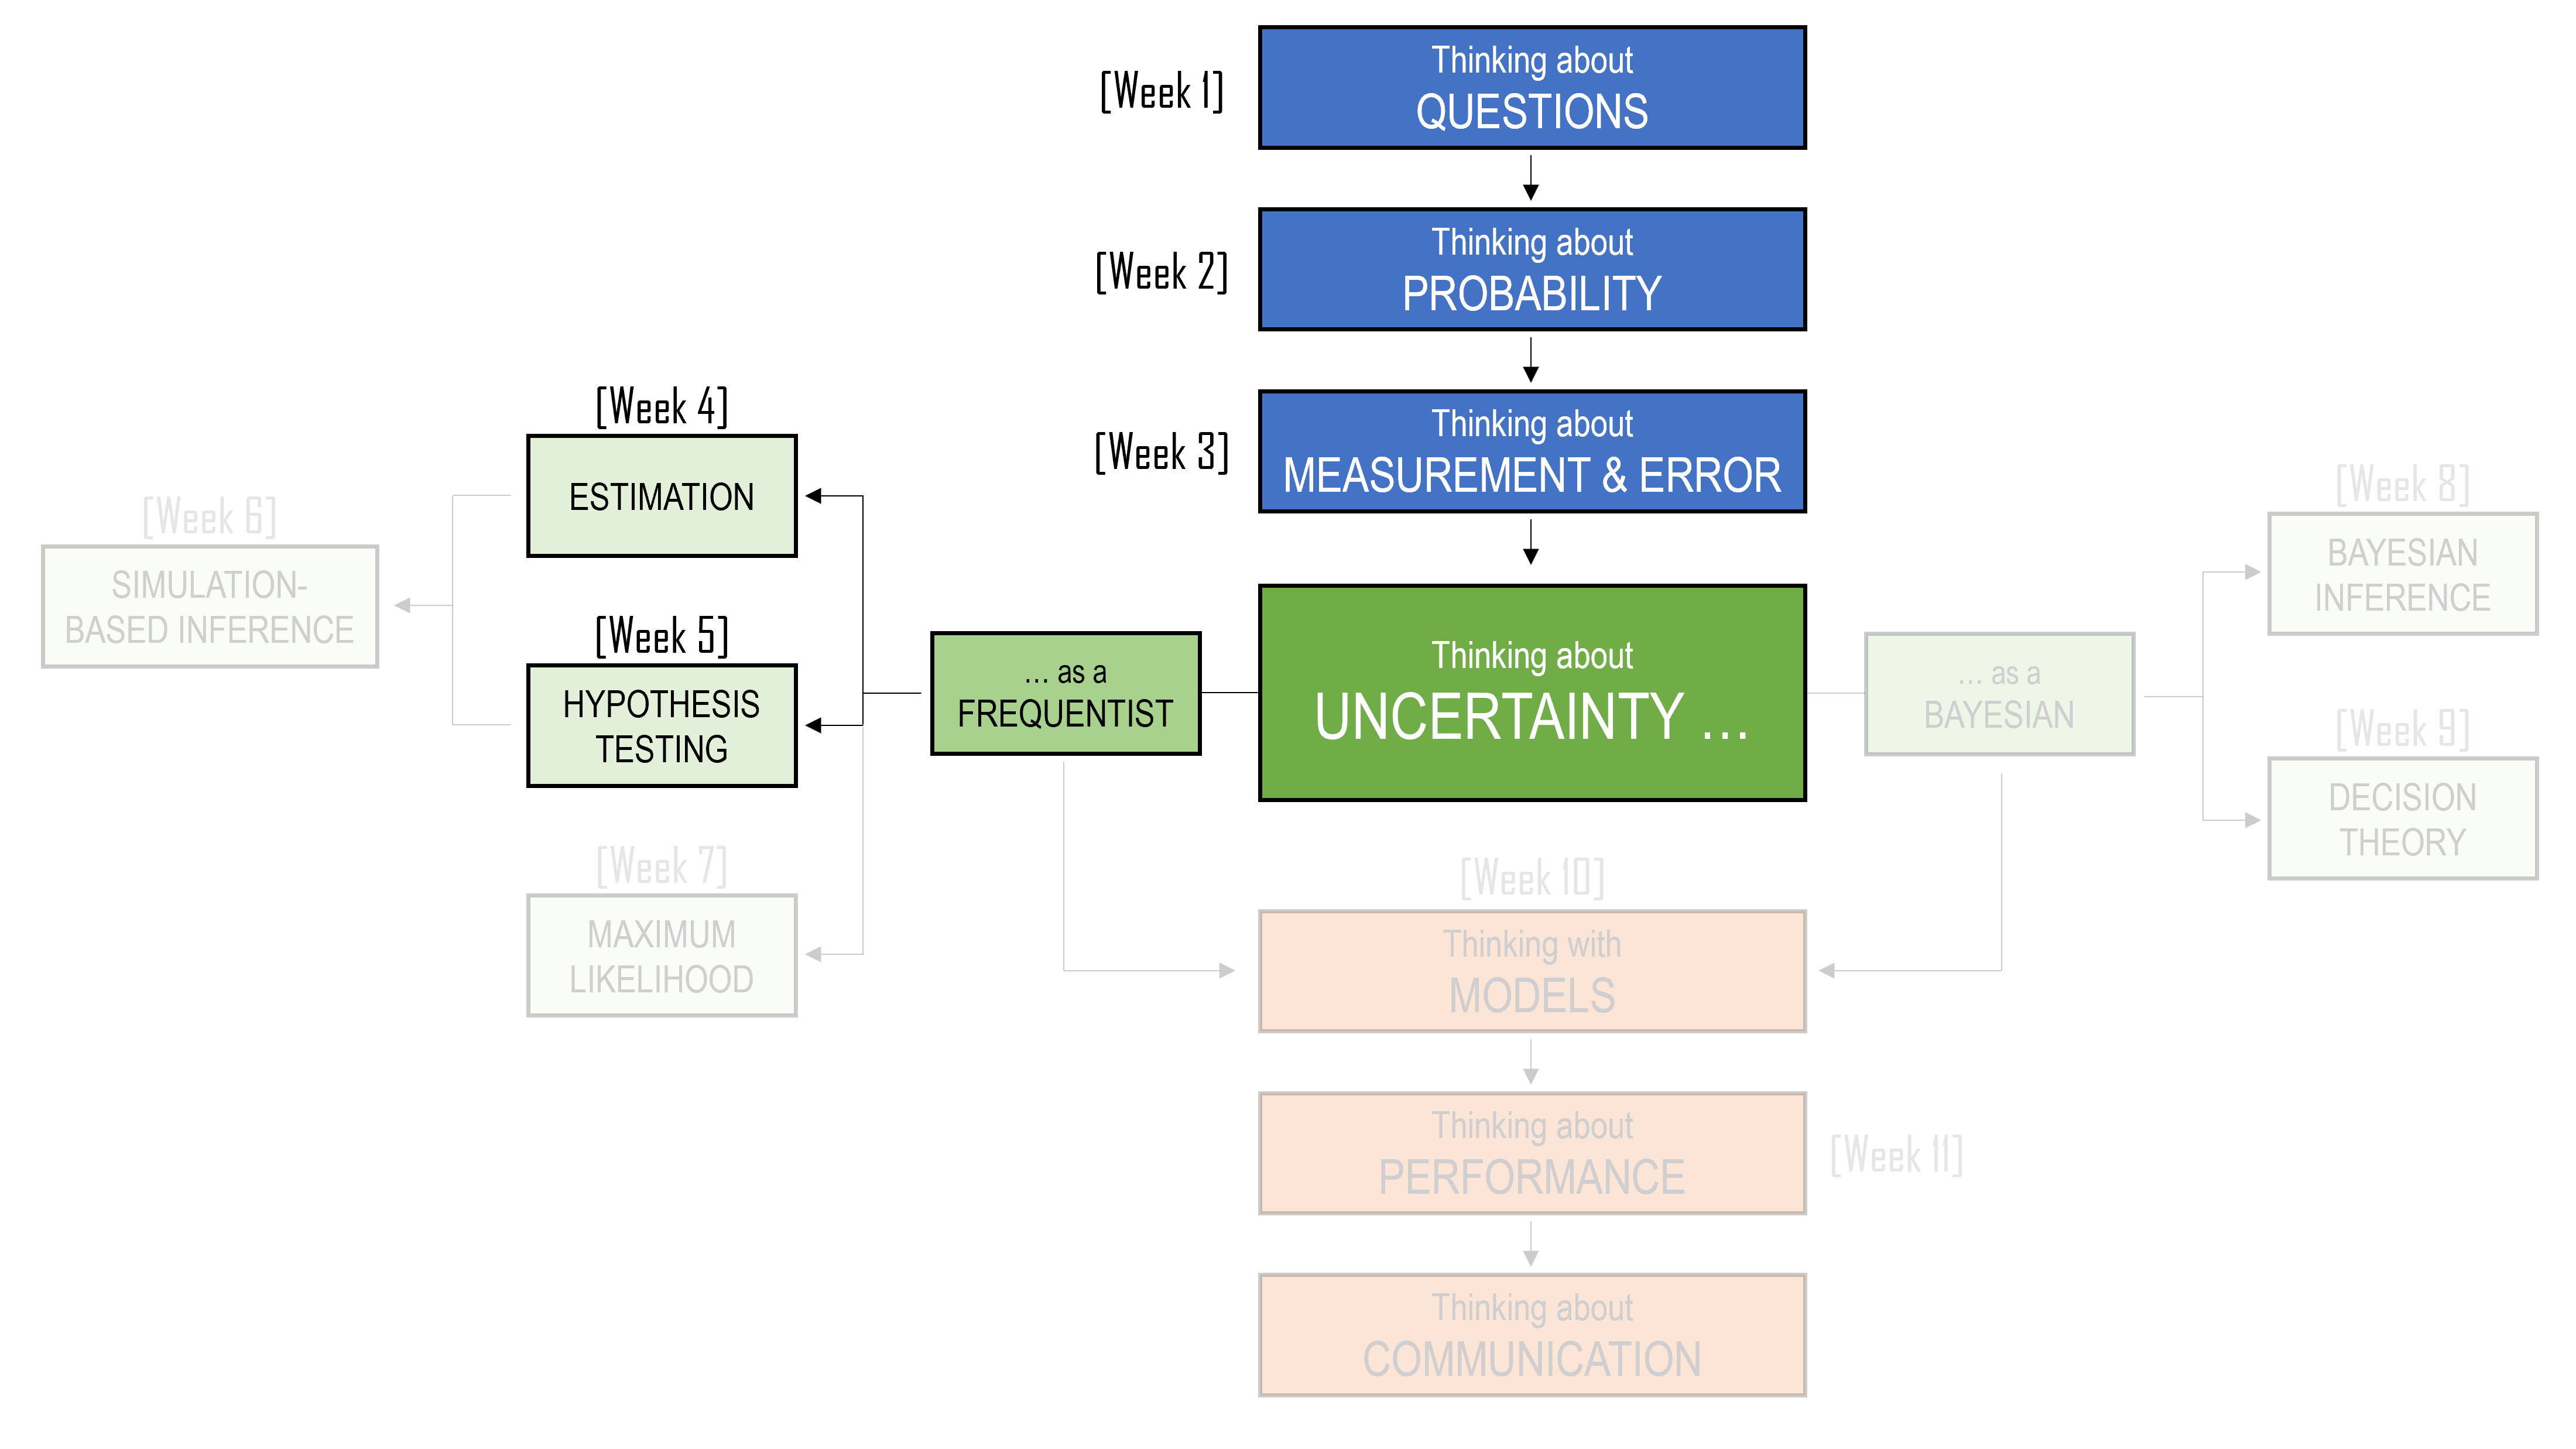
\includegraphics[width=14.67in,height=\textheight,keepaspectratio]{images/chapter5/outline.png}

\section{A famous cup of tea}\label{a-famous-cup-of-tea}

One of the most famous stories in statistics begins with a cup of tea.
The story is usually told like this.

\begin{quote}
At a summer afternoon tea party in Cambridge in the 1920s, a woman
claimed that she could tell whether milk had been poured into a cup
before the tea, or whether tea had been poured in before the milk. To
many people, this might have sounded like a small matter of personal
taste. Perhaps she preferred one method. Perhaps she was imagining the
difference. Perhaps she was simply confident.
\end{quote}

But the statistician, Ronald Fisher, saw something deeper in the claim.
The question was not whether she liked tea. The question was not whether
milk-first tea and tea-first tea tasted different to everyone. The
question was more precise:

\begin{quote}
Could this particular person distinguish between the two methods better
than would be expected by guessing?
\end{quote}

Imagine that we prepare eight cups of tea.

\begin{itemize}
\tightlist
\item
  Four are made by pouring the milk first, and four are made by pouring
  the tea first.
\item
  The cups are presented in random order.
\item
  The woman is told that there are four of each type.
\item
  She must identify which four had the milk poured first.
\end{itemize}

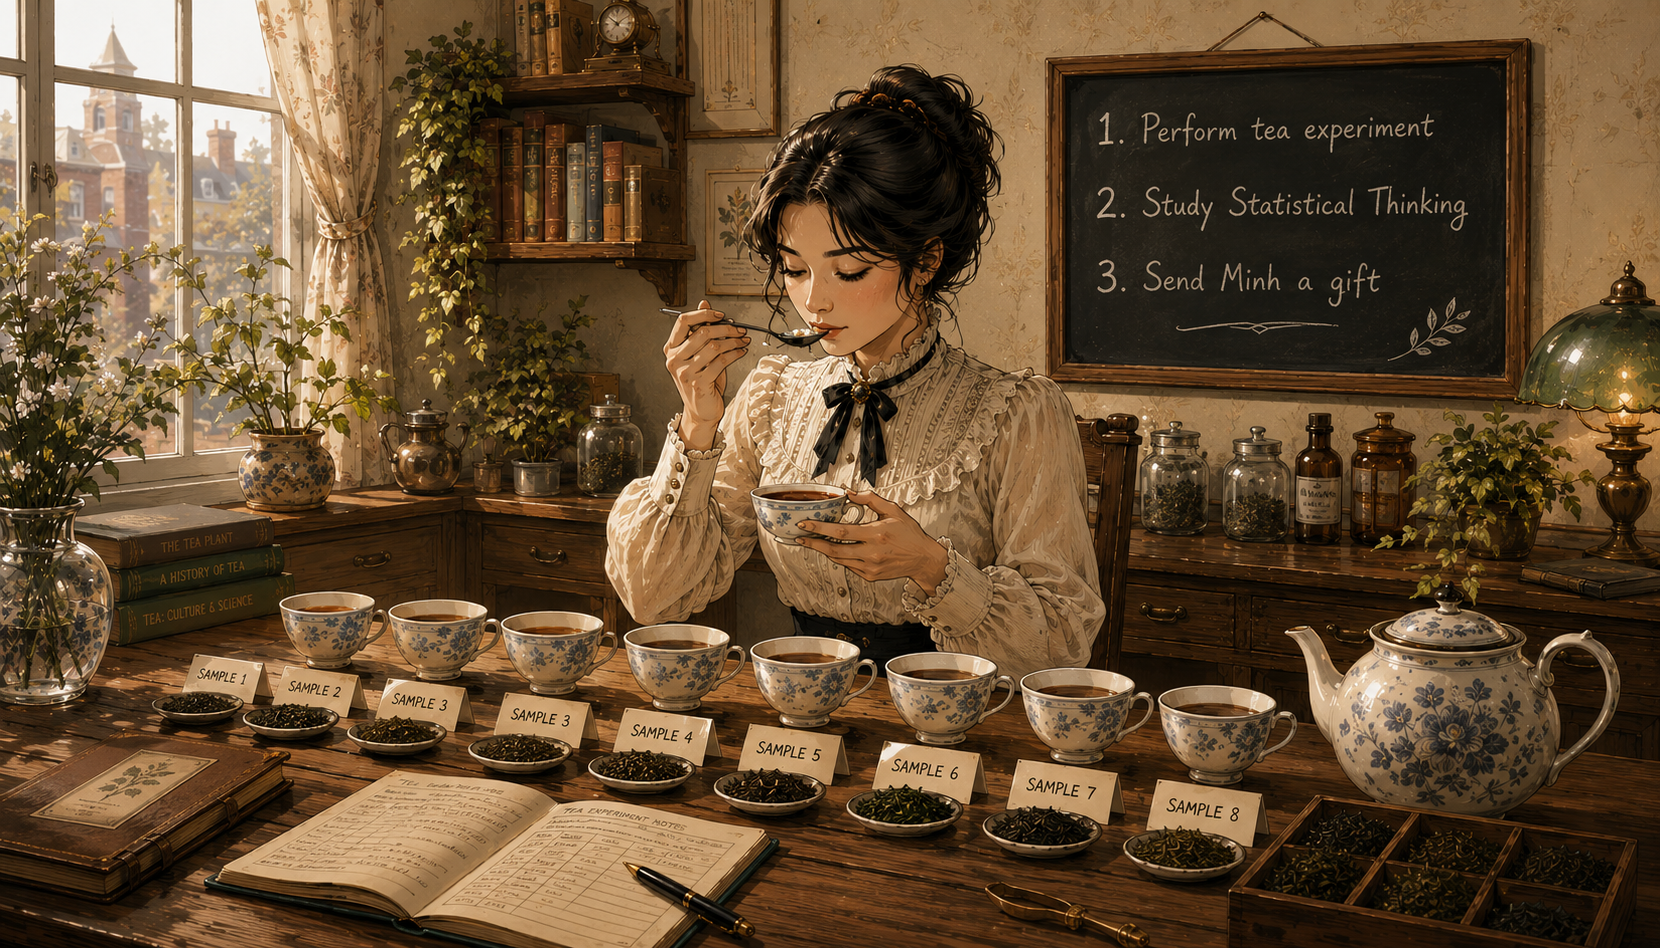
\includegraphics[width=5.53in,height=\textheight,keepaspectratio]{images/chapter5/tea.png}

There are many ways she could choose four cups out of eight. If she is
only guessing, she might still get some correct by chance. She might
even get all four correct by chance, although that would be rare.

That last point is important. A perfect score would not automatically
prove that she has a special ability. Chance can sometimes produce
surprising results. But if a perfect score would be very unlikely under
guessing, then the result may give us a reason to doubt the guessing
explanation.

So we begin with a skeptical view of her tea-tasting ability:

\[
\text{She is guessing}
\]

We then ask whether the result gives us evidence for a different
explanation:

\[
\text{She can distinguish between the two ways of preparing tea}
\]

The experiment does not begin by assuming that she is wrong in any moral
sense. Nor does it begin by assuming that she is right. Instead, it
begins with a benchmark model:

\begin{quote}
What would her results look like if she were only guessing?
\end{quote}

Under this guessing model, every possible selection of four cups is
equally likely. The number of ways to choose four cups from eight is:

\[
\binom{8}{4} = 70
\]

Only one of these 70 choices is perfectly correct. So, if she is
guessing, the probability of identifying all four milk-first cups
correctly is:

\[
\frac{1}{70} \approx 0.014
\]

That probability is small. It tells us that a perfect score would be
unusual if she were merely guessing. Although, this does not give us
certainty. It does not prove beyond all possible doubt that she can
taste the difference. But it gives us a disciplined way to compare two
explanations:

\begin{itemize}
\tightlist
\item
  perhaps she is only guessing;
\item
  perhaps she really can tell the difference.
\end{itemize}

The tea story also shows why the design of the test matters. Before
seeing the result, we need to decide what kind of outcome would count as
strong evidence. Would four correct identifications be enough? What
about three? Should we count only a perfect score, or should a nearly
perfect score also make us skeptical of the guessing explanation? These
choices need to be made before the cups are tasted. Otherwise, we risk
changing the rules after seeing the result.

This chapter is about that logic.

\section{Recap}\label{recap}

In the previous chapter, we began the formal study of statistical
inference. We used samples to estimate population quantities, and we
learned that an estimate is never the whole story. A sample mean, sample
median, or sample proportion may be useful, but it is still only one
number from one possible sample. Another sample could have produced a
different number.

In this chapter, we move from estimation to hypothesis testing. At
first, this may feel like a new topic. There will be new words: null
hypothesis, alternative hypothesis, test statistic, significance level,
p-value, Type I error, Type II error, and power. But the machinery
underneath is familiar. We are still thinking about samples,
populations, parameters, statistics, standard errors, and sampling
distributions.

The difference is the question we ask.

In estimation, we usually begin with the data and ask:

\begin{quote}
What population values are plausible?
\end{quote}

In hypothesis testing, we usually begin with a claim and ask:

\begin{quote}
Are the data surprising if that claim is true?
\end{quote}

For example, in the previous chapter we estimated average household
income. We also estimated differences between groups and proportions
below particular income thresholds. Now suppose someone makes a claim:

\begin{quote}
The average annual income of Australian households is \$100,000.
\end{quote}

Or:

\begin{quote}
The proportion of households with annual income below \$60,000 is 20\%.
\end{quote}

Or:

\begin{quote}
Mean household income is the same in capital city and regional areas.
\end{quote}

These are no longer just estimation questions. They are claims about a
population. Hypothesis testing gives us a formal way to compare such
claims with data.

\section{From estimation to testing}\label{from-estimation-to-testing}

Let us return to the running example from the previous chapter.

\begin{tcolorbox}[enhanced jigsaw, arc=.35mm, bottomrule=.15mm, bottomtitle=1mm, breakable, colback=white, colbacktitle=quarto-callout-note-color!10!white, colframe=quarto-callout-note-color-frame, coltitle=black, left=2mm, leftrule=.75mm, opacityback=0, opacitybacktitle=0.6, rightrule=.15mm, title=\textcolor{quarto-callout-note-color}{\faInfo}\hspace{0.5em}{Household income}, titlerule=0mm, toprule=.15mm, toptitle=1mm]

Suppose you work for the Australian Bureau of Statistics. You have been
asked to report on annual income for Australian households. In the
previous chapter, you used sample data to estimate population quantities
such as mean income, median income, the proportion of households below a
threshold, and the difference between regions.

Now suppose a report claims that the mean annual income of Australian
households is \$100,000.

Your sample mean is higher than this. Is the difference just sampling
variation, or does the sample provide evidence against the claim?

\end{tcolorbox}

This question sounds simple, but it contains the whole logic of
hypothesis testing.

The claim is about a \textbf{population parameter}. In this case, the
parameter is the population mean household income, which we write as:
\(\mu\).

The data give us a \textbf{sample statistic}. In this case, the
statistic is the sample mean, which we write as: \(\bar{x}\).

The sample statistic will almost never be exactly equal to the claimed
population value. If a report claims that the population mean is
\$100,000, and a sample gives a mean of \$101,200, that difference alone
is not interesting. Samples wobble. That is what we learned in the
previous chapter.

The real question is not:

\begin{quote}
Is the sample mean different from \$100,000?
\end{quote}

Of course it probably is. The better question is:

\begin{quote}
Is the sample mean far enough from \$100,000 that it would be unusual if
the true population mean really were \$100,000?
\end{quote}

This is where the ideas from estimation return.

\begin{table}
\fontsize{12.0pt}{14.0pt}\selectfont
\begin{tabular*}{\linewidth}{@{\extracolsep{\fill}}ll}
\toprule
Idea from estimation & Role in hypothesis testing \\ 
\midrule\addlinespace[2.5pt]
Population parameter & The unknown value appearing in the hypothesis \\ 
Sample statistic & The evidence used to assess the hypothesis \\ 
Sampling variation & The reason the statistic need not equal the hypothesised value exactly \\ 
Standard error & The scale used to judge whether a difference is large or small \\ 
Sampling distribution & The distribution of the statistic if the null hypothesis were true \\ 
Confidence interval & A related way to show which parameter values are plausible \\ 
\bottomrule
\end{tabular*}
\end{table}

\section{Research questions and
hypotheses}\label{research-questions-and-hypotheses}

A research question is usually written in ordinary language.

For example:

\begin{quote}
Is average household income different from \$100,000?
\end{quote}

or:

\begin{quote}
Is the proportion of households below \$60,000 greater than 20\%?
\end{quote}

or:

\begin{quote}
Do capital city households and regional households have different mean
incomes?
\end{quote}

A statistical hypothesis translates a question like this into a
statement about a population parameter.

A hypothesis is a statement about a population distribution or a
population parameter. In this chapter, we will mostly focus on
\emph{parametric hypotheses}, which are statements about parameters such
as means and proportions.

The two main hypotheses are:

\begin{itemize}
\tightlist
\item
  the \textbf{null hypothesis}, written as \(H_0\);
\item
  the \textbf{alternative hypothesis}, written as \(H_1\) or sometimes
  \(H_A\).
\end{itemize}

The null hypothesis usually represents a default position, a benchmark,
or a claim of no difference or no change. The alternative hypothesis
represents the effect or difference we are looking for evidence of.

For the mean household income claim, we might write:

\[
H_0: \mu = 100{,}000
\]

\[
H_1: \mu \neq 100{,}000.
\]

The null hypothesis says that the population mean is \$100,000. The
alternative says that it is not \$100,000.

Notice what these hypotheses are about. They are not about the sample
mean. They are not:

\[
H_0: \bar{x} = 100{,}000.
\]

That would not make sense as a population claim. Once we have the
sample, \(\bar{x}\) is known. The hypothesis is about the unknown
population mean \(\mu\). This distinction is important.

\begin{quote}
Hypotheses are about populations. Test statistics are calculated from
samples.
\end{quote}

\subsection{The role of the null
hypothesis}\label{the-role-of-the-null-hypothesis}

The null hypothesis has a special role. It is the position we assume for
the purpose of the test. We then ask whether the data look unusual under
that assumption. This can feel backwards. If we are interested in
whether mean household income is above \$100,000, why begin by assuming
it is exactly \$100,000?

One way to understand this is to think of the null as a skeptical
position. If someone claims that the mean is different from \$100,000,
we ask them to provide evidence. The null hypothesis is the position
that must be challenged.

This is similar to a court case. The starting point is not that the
defendant has proved innocence. The starting point is that guilt has not
been established. The prosecution must provide strong enough evidence to
move us away from the default position. In hypothesis testing, we do
something similar. We do not reject the null just because the sample
statistic is different from the null value. We reject the null only if
the difference is large relative to the sampling variation we would
expect.

\begin{tcolorbox}[enhanced jigsaw, arc=.35mm, bottomrule=.15mm, bottomtitle=1mm, breakable, colback=white, colbacktitle=quarto-callout-important-color!10!white, colframe=quarto-callout-important-color-frame, coltitle=black, left=2mm, leftrule=.75mm, opacityback=0, opacitybacktitle=0.6, rightrule=.15mm, title=\textcolor{quarto-callout-important-color}{\faExclamation}\hspace{0.5em}{Warning: We do not accept the null}, titlerule=0mm, toprule=.15mm, toptitle=1mm]

A hypothesis test has two possible outcomes:

\begin{enumerate}
\def\labelenumi{\arabic{enumi}.}
\tightlist
\item
  Reject \(H_0\).
\item
  Fail to reject \(H_0\).
\end{enumerate}

We do not usually say that we ``accept'' \(H_0\). Failing to reject the
null means that the data did not provide strong enough evidence against
it. It does not prove that the null hypothesis is true.

\end{tcolorbox}

\subsection{One-sided and two-sided
alternatives}\label{one-sided-and-two-sided-alternatives}

The alternative hypothesis should match the research question.

Sometimes we care about any difference from the null value. For example:

\begin{quote}
Is average household income different from \$100,000?
\end{quote}

This leads to a \textbf{two-sided} alternative:

\[
H_0: \mu = 100{,}000
\]

\[
H_1: \mu \neq 100{,}000
\]

The symbol \(\neq\) means ``not equal to''. This alternative includes
values below \$100,000 and values above \$100,000.

Sometimes we care about a specific direction. For example:

\begin{quote}
Is average household income higher than \$100,000?
\end{quote}

This leads to a \textbf{one-sided} alternative:

\[
H_0: \mu = 100{,}000
\]

\[
H_1: \mu > 100{,}000
\]

Or if the question is:

\begin{quote}
Is average household income lower than \$100,000?
\end{quote}

we would write:

\[
H_0: \mu = 100{,}000
\]

\[
H_1: \mu < 100{,}000
\]

The direction matters because it changes what counts as evidence against
the null.

If our alternative is \(\mu > 100{,}000\), then sample means much larger
than \$100,000 count as evidence against the null. Sample means much
smaller than \$100,000 do not support that particular alternative. They
may be surprising, but they are surprising in the wrong direction.

If our alternative is \(\mu \neq 100{,}000\), then sample means far
above or far below \$100,000 count as evidence against the null.

\begin{tcolorbox}[enhanced jigsaw, arc=.35mm, bottomrule=.15mm, bottomtitle=1mm, breakable, colback=white, colbacktitle=quarto-callout-important-color!10!white, colframe=quarto-callout-important-color-frame, coltitle=black, left=2mm, leftrule=.75mm, opacityback=0, opacitybacktitle=0.6, rightrule=.15mm, title=\textcolor{quarto-callout-important-color}{\faExclamation}\hspace{0.5em}{Warning: Choose the alternative before looking at the data}, titlerule=0mm, toprule=.15mm, toptitle=1mm]

The alternative hypothesis should be chosen before inspecting the sample
result. Choosing a one-sided test after seeing which direction the data
point is a form of changing the rules after the game has started.

\end{tcolorbox}

\section{Test statistics: measuring distance from the
null}\label{test-statistics-measuring-distance-from-the-null}

Suppose we collect a sample of \(n = 100\) households and obtain:

\[
\bar{x} = 105{,}000
\]

If the null hypothesis is:

\[
H_0: \mu = 100{,}000,
\]

then the sample mean is \$5,000 above the null value. But is \$5,000
large?

There is no way to answer that question from the difference alone. A
difference of \$5,000 might be large in a very precise survey. It might
be small in a small or highly variable survey. The missing ingredient is
the standard error.

In the previous chapter, the standard error told us how much a statistic
tends to wobble from sample to sample. In hypothesis testing, the
standard error gives us the scale for judging whether a difference from
the null is large or small.

The general form of many test statistics is:

\[
\text{test statistic}
=
\frac{\text{estimate} - \text{null value}}{\text{standard error}}
\]

For a one-sample mean, the test statistic is:

\[
t
=
\frac{\bar{x} - \mu_0}{s / \sqrt{n}},
\]

where:

\begin{itemize}
\tightlist
\item
  \(\bar{x}\) is the sample mean;
\item
  \(\mu_0\) is the value of \(\mu\) under the null hypothesis;
\item
  \(s\) is the sample standard deviation;
\item
  \(n\) is the sample size;
\item
  \(s/\sqrt{n}\) is the estimated standard error of the sample mean.
\end{itemize}

The test statistic tells us how many standard errors the estimate is
from the null value.

\begin{tcolorbox}[enhanced jigsaw, arc=.35mm, bottomrule=.15mm, bottomtitle=1mm, breakable, colback=white, colbacktitle=quarto-callout-note-color!10!white, colframe=quarto-callout-note-color-frame, coltitle=black, left=2mm, leftrule=.75mm, opacityback=0, opacitybacktitle=0.6, rightrule=.15mm, title=\textcolor{quarto-callout-note-color}{\faInfo}\hspace{0.5em}{A test statistic in words}, titlerule=0mm, toprule=.15mm, toptitle=1mm]

A test statistic is a standardised measure of disagreement between the
data and the null hypothesis. A value near zero means the estimate is
close to the null value. A large positive or negative value means the
estimate is far from the null value, measured in standard errors.

\end{tcolorbox}

Let us calculate a simple example.

Suppose:

\[
\bar{x} = 105{,}000,
\quad
\mu_0 = 100{,}000,
\quad
s = 40{,}000,
\quad
n = 100
\]

The standard error is:

\[
SE(\bar{x}) = \frac{40{,}000}{\sqrt{100}} = 4{,}000
\]

So the test statistic is:

\[
t
=
\frac{105{,}000 - 100{,}000}{4{,}000}
=
1.25
\]

The sample mean is 1.25 standard errors above the null value.

\begin{table}
\fontsize{12.0pt}{14.0pt}\selectfont
\begin{tabular*}{\linewidth}{@{\extracolsep{\fill}}lr}
\toprule
Quantity & Value \\ 
\midrule\addlinespace[2.5pt]
Sample mean & 105,000.00 \\ 
Null value & 100,000.00 \\ 
Sample standard deviation & 40,000.00 \\ 
Sample size & 100.00 \\ 
Standard error & 4,000.00 \\ 
Test statistic & 1.25 \\ 
\bottomrule
\end{tabular*}
\end{table}

This is the same logic as a confidence interval. In a confidence
interval, the standard error tells us how wide the interval should be.
In a hypothesis test, the standard error tells us how far the estimate
is from the null value.

\section{The sampling distribution under the
null}\label{the-sampling-distribution-under-the-null}

A test statistic is useful because we know, at least approximately, how
it should behave if the null hypothesis is true. This is where the
sampling distribution returns. In the previous chapter, we asked:

\begin{quote}
What would the sample mean look like across repeated samples?
\end{quote}

Now we ask a more specific question:

\begin{quote}
What would the sample mean look like across repeated samples if the null
hypothesis were true?
\end{quote}

Suppose the null hypothesis is:

\[
H_0: \mu = 100{,}000
\]

If this null hypothesis is true, and if our sample size is large enough
for the Central Limit Theorem to be useful, then repeated sample means
should vary around \$100,000. Most sample means should be reasonably
close to \$100,000. A few will be far away just by chance.

The hypothesis test asks whether our observed sample mean is ordinary or
unusual under this imagined world.

\pandocbounded{
\includegraphics[keepaspectratio]{5_HypothesisTesting_files/figure-pdf/unnamed-chunk-6-1.pdf}}

The plot shows the idea behind the test. We are not asking whether the
observed sample mean equals the null value. We are asking \textbf{where}
the observed sample mean falls in the sampling distribution that would
be expected if the null hypothesis were true.

\begin{itemize}
\tightlist
\item
  If the observed statistic is near the centre of this distribution, it
  is compatible with the null.
\item
  If it is far out in the tail, it is less compatible with the null.
\end{itemize}

This is the repeated-sampling logic of hypothesis testing.

\section{Critical regions and significance
levels}\label{critical-regions-and-significance-levels}

A hypothesis test can be described as a decision rule. A test statistic
is a statistic used to assess the null hypothesis. A critical region is
the set of values of the test statistic for which we reject the null
hypothesis. For example, suppose a test statistic \(T\) tends to be near
zero when the null hypothesis is true. Large positive values are
evidence against the null. Then a possible decision rule is:

\[
\text{Reject } H_0 \text{ if } T > c
\]

The number \(c\) is the critical value. The critical region is the set
of values greater than \(c\). How should we choose \(c\)?

One common approach is to choose a significance level, written as
\(\alpha\). The significance level is the probability of rejecting the
null hypothesis when the null hypothesis is true.

\[
\alpha = P(\text{reject } H_0 \mid H_0 \text{ is true})
\]

This is also the probability of a Type I error, which we will discuss in
more detail later.

A very common choice is:

\[
\alpha = 0.05
\]

A 5\% significance level means that, if the null hypothesis were true
and we repeated the testing procedure many times, we would reject the
null about 5\% of the time.

\begin{tcolorbox}[enhanced jigsaw, arc=.35mm, bottomrule=.15mm, bottomtitle=1mm, breakable, colback=white, colbacktitle=quarto-callout-important-color!10!white, colframe=quarto-callout-important-color-frame, coltitle=black, left=2mm, leftrule=.75mm, opacityback=0, opacitybacktitle=0.6, rightrule=.15mm, title=\textcolor{quarto-callout-important-color}{\faExclamation}\hspace{0.5em}{Warning: The 5\% level is a convention}, titlerule=0mm, toprule=.15mm, toptitle=1mm]

There is nothing magical about 0.05. It is a common convention, not a
law of nature. In some settings, a smaller or larger significance level
may be more appropriate. The choice should depend on the consequences of
the possible errors.

\end{tcolorbox}

For a two-sided test using a standard normal approximation, the 5\%
critical region is roughly:

\[
|Z| > 1.96
\]

This means that we reject the null if the test statistic is more than
1.96 standard errors below the null value or more than 1.96 standard
errors above it.

\pandocbounded{
\includegraphics[keepaspectratio]{5_HypothesisTesting_files/figure-pdf/unnamed-chunk-7-1.pdf}}

The critical region gives a rule. If the observed test statistic lands
in the shaded area, we reject \(H_0\). If it does not, we fail to reject
\(H_0\).

\section{P-values}\label{p-values}

The critical-region approach is useful because it makes the decision
rule clear. But in practice, hypothesis tests are often reported using
\textbf{p-values}.

A p-value asks:

\begin{quote}
If the null hypothesis were true, how likely would it be to observe a
test statistic as extreme as, or more extreme than, the one we actually
observed?
\end{quote}

This definition is worth reading slowly.

The p-value is calculated \textbf{assuming the null hypothesis is true}.
It is not the probability that the null hypothesis is true.

For example, suppose we test:

\[
H_0: \mu = 100{,}000
\]

against:

\[
H_1: \mu \neq 100{,}000
\]

And suppose the observed test statistic is:

\[
t = 2.29.
\]

For a two-sided test, values at least as extreme as \(2.29\) include
values greater than \(2.29\) and values less than \(-2.29\). The p-value
is the probability, under the null distribution, of landing in either
tail.

In R, using a \(t\) distribution with 99 degrees of freedom:

\begin{Shaded}
\begin{Highlighting}[]
\DecValTok{2} \SpecialCharTok{*} \FunctionTok{pt}\NormalTok{(}\SpecialCharTok{{-}}\FunctionTok{abs}\NormalTok{(}\FloatTok{2.29}\NormalTok{), }\AttributeTok{df =} \DecValTok{99}\NormalTok{)}
\end{Highlighting}
\end{Shaded}

\begin{verbatim}
[1] 0.02414349
\end{verbatim}

This gives a p-value of about 0.024.

At the 5\% significance level, we would reject \(H_0\) because:

\[
p\text{-value} < 0.05
\]

At the 1\% significance level, we would not reject \(H_0\) because:

\[
p\text{-value} > 0.01
\]

This is why it is often more informative to report the p-value than only
saying ``significant'' or ``not significant''. The p-value gives more
detail about the strength of disagreement between the data and the null
model.

But it must be interpreted carefully.

\begin{tcolorbox}[enhanced jigsaw, arc=.35mm, bottomrule=.15mm, bottomtitle=1mm, breakable, colback=white, colbacktitle=quarto-callout-important-color!10!white, colframe=quarto-callout-important-color-frame, coltitle=black, left=2mm, leftrule=.75mm, opacityback=0, opacitybacktitle=0.6, rightrule=.15mm, title=\textcolor{quarto-callout-important-color}{\faExclamation}\hspace{0.5em}{Warning: What a p-value is not}, titlerule=0mm, toprule=.15mm, toptitle=1mm]

A p-value is not:

\begin{itemize}
\tightlist
\item
  the probability that the null hypothesis is true;
\item
  the probability that the alternative hypothesis is true;
\item
  the probability that the result is due to chance;
\item
  the size of the effect;
\item
  proof that the null hypothesis is false.
\end{itemize}

A small p-value means that the observed data would be unusual if the
null hypothesis were true.

\end{tcolorbox}

A useful way to say it is:

\begin{quote}
A p-value measures compatibility between the data and the null model.
Smaller p-values indicate less compatibility.
\end{quote}

\section{A one-sample t-test for mean household
income}\label{a-one-sample-t-test-for-mean-household-income}

Let us now work through a full example.

\begin{tcolorbox}[enhanced jigsaw, arc=.35mm, bottomrule=.15mm, bottomtitle=1mm, breakable, colback=white, colbacktitle=quarto-callout-note-color!10!white, colframe=quarto-callout-note-color-frame, coltitle=black, left=2mm, leftrule=.75mm, opacityback=0, opacitybacktitle=0.6, rightrule=.15mm, title=\textcolor{quarto-callout-note-color}{\faInfo}\hspace{0.5em}{Mean household income}, titlerule=0mm, toprule=.15mm, toptitle=1mm]

A report claims that the mean annual income of Australian households is
\$100,000. A sample of 100 households gives a sample mean of \$108,000
and a sample standard deviation of \$35,000.

Is there evidence that the population mean is different from \$100,000?

\end{tcolorbox}

The population parameter is:

\[
\mu = \text{mean annual income of all Australian households}
\]

The null and alternative hypotheses are:

\[
H_0: \mu = 100{,}000
\]

\[
H_1: \mu \neq 100{,}000
\]

The sample information is:

\[
\bar{x} = 108{,}000,
\quad
s = 35{,}000,
\quad
n = 100
\]

The standard error is:

\[
SE(\bar{x})
=
\frac{s}{\sqrt{n}}
=
\frac{35{,}000}{\sqrt{100}}
=
3{,}500
\]

The test statistic is:

\[
t
=
\frac{\bar{x} - \mu_0}{s/\sqrt{n}}
=
\frac{108{,}000 - 100{,}000}{3{,}500}
=
2.286
\]

The degrees of freedom are:

\[
n - 1 = 99
\]

The two-sided p-value is:

\begin{Shaded}
\begin{Highlighting}[]
\NormalTok{xbar }\OtherTok{\textless{}{-}} \DecValTok{108000}
\NormalTok{mu0 }\OtherTok{\textless{}{-}} \DecValTok{100000}
\NormalTok{s }\OtherTok{\textless{}{-}} \DecValTok{35000}
\NormalTok{n }\OtherTok{\textless{}{-}} \DecValTok{100}
\NormalTok{se }\OtherTok{\textless{}{-}}\NormalTok{ s }\SpecialCharTok{/} \FunctionTok{sqrt}\NormalTok{(n)}
\NormalTok{t\_obs }\OtherTok{\textless{}{-}}\NormalTok{ (xbar }\SpecialCharTok{{-}}\NormalTok{ mu0) }\SpecialCharTok{/}\NormalTok{ se}
\NormalTok{p\_value }\OtherTok{\textless{}{-}} \DecValTok{2} \SpecialCharTok{*} \FunctionTok{pt}\NormalTok{(}\SpecialCharTok{{-}}\FunctionTok{abs}\NormalTok{(t\_obs), }\AttributeTok{df =}\NormalTok{ n }\SpecialCharTok{{-}} \DecValTok{1}\NormalTok{)}
\end{Highlighting}
\end{Shaded}

\begin{table}
\fontsize{12.0pt}{14.0pt}\selectfont
\begin{tabular*}{\linewidth}{@{\extracolsep{\fill}}rrrrrr}
\toprule
Sample mean & Null value & Standard error & Test statistic & Degrees of freedom & p-value \\ 
\midrule\addlinespace[2.5pt]
\$108,000 & \$100,000 & \$3,500 & 2.286 & 99 & 0.024 \\ 
\bottomrule
\end{tabular*}
\end{table}

The p-value is about 0.024. At the 5\% significance level, we reject the
null hypothesis.

A careful conclusion would be:

\begin{quote}
The sample provides evidence that the mean annual household income
differs from \$100,000. The sample mean was \$108,000, and the
difference from \$100,000 was large relative to the estimated standard
error.
\end{quote}

It is also incomplete to report only the p-value. We should report the
estimate and uncertainty as well.

The corresponding 95\% confidence interval is:

\begin{Shaded}
\begin{Highlighting}[]
\NormalTok{multiplier }\OtherTok{\textless{}{-}} \FunctionTok{qt}\NormalTok{(}\FloatTok{0.975}\NormalTok{, }\AttributeTok{df =}\NormalTok{ n }\SpecialCharTok{{-}} \DecValTok{1}\NormalTok{)}
\NormalTok{lower }\OtherTok{\textless{}{-}}\NormalTok{ xbar }\SpecialCharTok{{-}}\NormalTok{ multiplier }\SpecialCharTok{*}\NormalTok{ se}
\NormalTok{upper }\OtherTok{\textless{}{-}}\NormalTok{ xbar }\SpecialCharTok{+}\NormalTok{ multiplier }\SpecialCharTok{*}\NormalTok{ se}
\end{Highlighting}
\end{Shaded}

\begin{table}
\fontsize{12.0pt}{14.0pt}\selectfont
\begin{tabular*}{\linewidth}{@{\extracolsep{\fill}}rrr}
\toprule
Estimate & Lower & Upper \\ 
\midrule\addlinespace[2.5pt]
\$108,000 & \$101,055 & \$114,945 \\ 
\bottomrule
\end{tabular*}
\end{table}

This interval gives a fuller picture. It shows not only that \$100,000
lies outside the interval, but also which values are reasonably
compatible with the data.

\section{Confidence intervals and hypothesis
tests}\label{confidence-intervals-and-hypothesis-tests}

The connection between confidence intervals and hypothesis tests is
important. For a two-sided test at the 5\% significance level, testing:

\[
H_0: \mu = \mu_0
\]

is closely related to checking whether \(\mu_0\) lies inside or outside
the 95\% confidence interval.

\begin{itemize}
\tightlist
\item
  If \(\mu_0\) lies outside the 95\% confidence interval, the two-sided
  5\% test rejects \(H_0\).
\item
  If \(\mu_0\) lies inside the 95\% confidence interval, the two-sided
  5\% test does not reject \(H_0\).
\end{itemize}

In the previous example, the 95\% confidence interval was approximately:

\[
(101{,}056,\ 114{,}944)
\]

The null value \$100,000 is outside this interval. So the two-sided 5\%
test rejects:

\[
H_0: \mu = 100{,}000
\]

This connection can help you interpret both tools. But the confidence
interval is usually more informative. The test asks whether one value is
hard to believe. The interval shows a range of values that remain
plausible.

\section{Two-sample t-tests}\label{two-sample-t-tests}

Now suppose we want to compare two groups.

In the previous chapter, we estimated the difference in mean household
income between capital city and regional households. Here we turn that
into a hypothesis test.

\begin{tcolorbox}[enhanced jigsaw, arc=.35mm, bottomrule=.15mm, bottomtitle=1mm, breakable, colback=white, colbacktitle=quarto-callout-note-color!10!white, colframe=quarto-callout-note-color-frame, coltitle=black, left=2mm, leftrule=.75mm, opacityback=0, opacitybacktitle=0.6, rightrule=.15mm, title=\textcolor{quarto-callout-note-color}{\faInfo}\hspace{0.5em}{Household income in two regions}, titlerule=0mm, toprule=.15mm, toptitle=1mm]

Suppose we collect annual income data from households in capital city
areas and regional areas.

We want to know whether the mean income differs between the two
populations.

\end{tcolorbox}

Let: \(\mu_{\text{capital}}\) be the population mean income for capital
city households, and let: \(\mu_{\text{regional}}\) be the population
mean income for regional households.

The estimation question is:

\begin{quote}
How large is the difference between the two means?
\end{quote}

The hypothesis testing question is:

\begin{quote}
Is there evidence that the two population means differ?
\end{quote}

The hypotheses for a two-sided test are:

\[
H_0: \mu_{\text{capital}} - \mu_{\text{regional}} = 0
\]

\[
H_1: \mu_{\text{capital}} - \mu_{\text{regional}} \neq 0
\]

Equivalently, we could write:

\[
H_0: \mu_{\text{capital}} = \mu_{\text{regional}}
\]

\[
H_1: \mu_{\text{capital}} \neq \mu_{\text{regional}}
\]

Let us create a sample dataset to illustrate the calculation.

\begin{table}
\fontsize{12.0pt}{14.0pt}\selectfont
\begin{tabular*}{\linewidth}{@{\extracolsep{\fill}}lrrr}
\toprule
region & n & Sample mean & Sample standard deviation \\ 
\midrule\addlinespace[2.5pt]
Capital city & 80 & \$104,609 & \$58,395 \\ 
Regional & 80 & \$84,649 & \$43,412 \\ 
\bottomrule
\end{tabular*}
\end{table}

The sample means differ, but again we must ask whether the difference is
large relative to its standard error.

For two independent samples, a common test statistic is:

\[
t
=
\frac{\bar{x}_{\text{capital}} - \bar{x}_{\text{regional}}}
{\sqrt{s^2_{\text{capital}}/n_{\text{capital}} + s^2_{\text{regional}}/n_{\text{regional}}}}
\]

This version is called Welch's two-sample t-test. It does not require us
to assume that the two population variances are equal.

We usually let R calculate the details, including the degrees of
freedom.

\begin{Shaded}
\begin{Highlighting}[]
\FunctionTok{t.test}\NormalTok{(income }\SpecialCharTok{\textasciitilde{}}\NormalTok{ region, }\AttributeTok{data =}\NormalTok{ income\_regions)}
\end{Highlighting}
\end{Shaded}

\begin{verbatim}

    Welch Two Sample t-test

data:  income by region
t = 2.4535, df = 145.89, p-value = 0.01532
alternative hypothesis: true difference in means between group Capital city and group Regional is not equal to 0
95 percent confidence interval:
  3881.81 36038.19
sample estimates:
mean in group Capital city     mean in group Regional 
                 104608.75                   84648.75 
\end{verbatim}

The output includes:

\begin{itemize}
\tightlist
\item
  the test statistic;
\item
  the degrees of freedom;
\item
  the p-value;
\item
  a confidence interval for the difference in means;
\item
  the two sample means.
\end{itemize}

This is useful because it reminds us that the test is not separate from
estimation. The same output gives both a decision and an interval
estimate.

If our research question were directional, we could use a one-sided
test. For example:

\begin{quote}
Is mean household income higher in capital city areas than in regional
areas?
\end{quote}

Then the alternative would be:

\[
H_1: \mu_{\text{capital}} - \mu_{\text{regional}} > 0
\]

In R, the direction depends on how the groups are ordered. It is often
clearer to create two objects and then use them directly.

\begin{Shaded}
\begin{Highlighting}[]
\NormalTok{capital\_income }\OtherTok{\textless{}{-}}\NormalTok{ income\_regions }\SpecialCharTok{|\textgreater{}}
  \FunctionTok{filter}\NormalTok{(region }\SpecialCharTok{==} \StringTok{"Capital city"}\NormalTok{) }\SpecialCharTok{|\textgreater{}}
  \FunctionTok{pull}\NormalTok{(income)}

\NormalTok{regional\_income }\OtherTok{\textless{}{-}}\NormalTok{ income\_regions }\SpecialCharTok{|\textgreater{}}
  \FunctionTok{filter}\NormalTok{(region }\SpecialCharTok{==} \StringTok{"Regional"}\NormalTok{) }\SpecialCharTok{|\textgreater{}}
  \FunctionTok{pull}\NormalTok{(income)}

\FunctionTok{t.test}\NormalTok{(capital\_income, regional\_income, }\AttributeTok{alternative =} \StringTok{"greater"}\NormalTok{)}
\end{Highlighting}
\end{Shaded}

\begin{verbatim}

    Welch Two Sample t-test

data:  capital_income and regional_income
t = 2.4535, df = 145.89, p-value = 0.007662
alternative hypothesis: true difference in means is greater than 0
95 percent confidence interval:
 6493.17     Inf
sample estimates:
mean of x mean of y 
104608.75  84648.75 
\end{verbatim}

\section{Paired samples t-test}\label{paired-samples-t-test}

Not all comparisons involve two independent groups. Sometimes each
observation in one group is naturally paired with an observation in
another group. When data are paired, the analysis should use the
pairing.

\begin{tcolorbox}[enhanced jigsaw, arc=.35mm, bottomrule=.15mm, bottomtitle=1mm, breakable, colback=white, colbacktitle=quarto-callout-note-color!10!white, colframe=quarto-callout-note-color-frame, coltitle=black, left=2mm, leftrule=.75mm, opacityback=0, opacitybacktitle=0.6, rightrule=.15mm, title=\textcolor{quarto-callout-note-color}{\faInfo}\hspace{0.5em}{Income before and after housing costs}, titlerule=0mm, toprule=.15mm, toptitle=1mm]

Suppose we record household income before housing costs and disposable
income after housing costs for the same households.

Each household contributes two values. These values are paired because
they come from the same household.

\end{tcolorbox}

In a paired design, we reduce the problem to a one-sample problem by
calculating differences.

Let:

\[
D_i = X_i - Y_i,
\]

where:

\begin{itemize}
\tightlist
\item
  \(X_i\) is income before housing costs for household \(i\);
\item
  \(Y_i\) is income after housing costs for household \(i\);
\item
  \(D_i\) is the difference for household \(i\).
\end{itemize}

If we want to test whether income before housing costs is higher than
income after housing costs, we test:

\[
H_0: \mu_D = 0
\]

\[
H_1: \mu_D > 0
\]

The paired t-test is just a one-sample t-test applied to the
differences.

\begin{table}
\fontsize{12.0pt}{14.0pt}\selectfont
\begin{tabular*}{\linewidth}{@{\extracolsep{\fill}}rrrr}
\toprule
n & Mean before housing costs & Mean after housing costs & Mean difference \\ 
\midrule\addlinespace[2.5pt]
40 & \$88,230 & \$65,123 & \$23,108 \\ 
\bottomrule
\end{tabular*}
\end{table}

We can run the paired test in R:

\begin{Shaded}
\begin{Highlighting}[]
\FunctionTok{t.test}\NormalTok{(housing\_data}\SpecialCharTok{$}\NormalTok{before\_housing, }
\NormalTok{       housing\_data}\SpecialCharTok{$}\NormalTok{after\_housing, }
       \AttributeTok{paired =} \ConstantTok{TRUE}\NormalTok{, }
       \AttributeTok{alternative =} \StringTok{"greater"}\NormalTok{)}
\end{Highlighting}
\end{Shaded}

\begin{verbatim}

    Paired t-test

data:  housing_data$before_housing and housing_data$after_housing
t = 18.237, df = 39, p-value < 2.2e-16
alternative hypothesis: true mean difference is greater than 0
95 percent confidence interval:
 20972.65      Inf
sample estimates:
mean difference 
        23107.5 
\end{verbatim}

Or we can calculate the differences ourselves and run a one-sample
t-test:

\begin{Shaded}
\begin{Highlighting}[]
\FunctionTok{t.test}\NormalTok{(housing\_data}\SpecialCharTok{$}\NormalTok{difference, }
       \AttributeTok{mu =} \DecValTok{0}\NormalTok{, }
       \AttributeTok{alternative =} \StringTok{"greater"}\NormalTok{)}
\end{Highlighting}
\end{Shaded}

\begin{verbatim}

    One Sample t-test

data:  housing_data$difference
t = 18.237, df = 39, p-value < 2.2e-16
alternative hypothesis: true mean is greater than 0
95 percent confidence interval:
 20972.65      Inf
sample estimates:
mean of x 
  23107.5 
\end{verbatim}

These give the same test, because the paired test is a test of the mean
difference.

\section{Type I error and Type II
error}\label{type-i-error-and-type-ii-error}

So far, we have described hypothesis testing as a procedure for deciding
whether to reject the null hypothesis. But any decision made from
uncertain data can be wrong.

There are two main kinds of error.

\begin{itemize}
\tightlist
\item
  A \textbf{Type I error} occurs when we reject the null hypothesis even
  though it is true.
\item
  A \textbf{Type II error} occurs when we fail to reject the null
  hypothesis even though it is false.
\end{itemize}

\begin{table}
\fontsize{12.0pt}{14.0pt}\selectfont
\begin{tabular*}{\linewidth}{@{\extracolsep{\fill}}lll}
\toprule
Reality & Decision & Outcome \\ 
\midrule\addlinespace[2.5pt]
\(H_0\) is true & Fail to reject \(H_0\) & Correct decision \\ 
\(H_0\) is true & Reject \(H_0\) & Type I error \\ 
\(H_0\) is false & Fail to reject \(H_0\) & Type II error \\ 
\(H_0\) is false & Reject \(H_0\) & Correct decision \\ 
\bottomrule
\end{tabular*}
\end{table}

Let us put this in context.

\begin{tcolorbox}[enhanced jigsaw, arc=.35mm, bottomrule=.15mm, bottomtitle=1mm, breakable, colback=white, colbacktitle=quarto-callout-note-color!10!white, colframe=quarto-callout-note-color-frame, coltitle=black, left=2mm, leftrule=.75mm, opacityback=0, opacitybacktitle=0.6, rightrule=.15mm, title=\textcolor{quarto-callout-note-color}{\faInfo}\hspace{0.5em}{A policy threshold}, titlerule=0mm, toprule=.15mm, toptitle=1mm]

Suppose a government agency will introduce additional financial support
in a region if there is strong evidence that more than 25\% of
households have annual income below \$60,000.

\end{tcolorbox}

The hypotheses might be:

\[
H_0: p = 0.25
\]

\[
H_1: p > 0.25
\]

A Type I error would occur if the true proportion were 25\%, but the
sample led us to reject \(H_0\) and conclude that the proportion was
higher. The agency might allocate extra support to a region that did not
actually exceed the threshold.

A Type II error would occur if the true proportion were higher than
25\%, but the sample did not lead us to reject \(H_0\). The agency might
fail to provide extra support to a region that did actually exceed the
threshold.

Which error is worse?

There is no purely statistical answer. It depends on the context. If
resources are limited, a Type I error may direct support away from other
regions. If the consequences of missing need are severe, a Type II error
may be more harmful.

This is why the significance level is not just a technical detail. It
reflects how we balance errors.

The probability of a Type I error is:

\[
\alpha = P(\text{reject } H_0 \mid H_0 \text{ is true})
\]

The probability of a Type II error is:

\[
\beta = P(\text{fail to reject } H_0 \mid H_0 \text{ is false})
\]

The \textbf{power} of a test is:

\[
1 - \beta = P(\text{reject } H_0 \mid H_0 \text{ is false})
\]

Power is the probability of detecting an effect when the effect is
really there.

\section{Statistical significance and practical
importance}\label{statistical-significance-and-practical-importance}

A statistically significant result is not necessarily an important
result. This is one of the most common misunderstandings in applied
statistics. Suppose a very large survey finds that mean household income
is \$1,200 higher in capital city areas than in regional areas, with a
p-value below 0.001. The result may be statistically significant because
the sample size is large. With enough data, even very small differences
can become difficult to explain by sampling variation alone.

But is \$1,200 per year practically important?

The answer depends on context. For some households, \$1,200 may matter a
great deal. For a broad comparison of regional economic conditions, it
may or may not be the main issue. The p-value alone cannot answer that
question.

Now consider the opposite case. Suppose a small survey estimates that
mean household income is \$12,000 lower in one region, but the p-value
is 0.09. This is not statistically significant at the 5\% level. But the
estimated difference may still be practically important. The study may
simply be too small to estimate the difference precisely.

\begin{table}
\fontsize{12.0pt}{14.0pt}\selectfont
\begin{tabular*}{\linewidth}{@{\extracolsep{\fill}}lrll}
\toprule
Scenario & Estimated difference & p-value & Careful interpretation \\ 
\midrule\addlinespace[2.5pt]
Very large sample, small estimated difference & \$1,200 & <0.001 & Strong statistical evidence, but practical importance still needs context. \\ 
Small sample, large estimated difference & \$12,000 & 0.09 & Not statistically significant at 5\%, but the possible effect may still matter. \\ 
\bottomrule
\end{tabular*}
\end{table}

The word ``significant'' is dangerous because in ordinary language it
means important. In statistics, significant means something narrower:
the result crossed a threshold in a hypothesis test.

\subsection{Common misinterpretations}\label{common-misinterpretations}

Hypothesis testing is widely used, but it is also widely misinterpreted.
Many mistakes come from treating the p-value as if it answers a question
it does not answer.

\begin{table}
\fontsize{12.0pt}{14.0pt}\selectfont
\begin{tabular*}{\linewidth}{@{\extracolsep{\fill}}ll}
\toprule
Misinterpretation & Better interpretation \\ 
\midrule\addlinespace[2.5pt]
The p-value is the probability that \(H_0\) is true. & The p-value is calculated assuming \(H_0\) is true. \\ 
A small p-value proves that \(H_0\) is false. & A small p-value says the data are unusual under the null model. \\ 
A large p-value proves that there is no effect. & A large p-value means the data did not provide strong evidence against \(H_0\). \\ 
Statistical significance means practical importance. & Importance depends on the size of the estimate and the context. \\ 
A non-significant result means the groups are the same. & The study may not have had enough power to detect a difference. \\ 
The 5\% level is a magic boundary. & The 5\% level is a convention, not a natural law. \\ 
\bottomrule
\end{tabular*}
\end{table}

Let us apply this to the household income example.

Suppose we test:

\[
H_0: \mu_{\text{capital}} = \mu_{\text{regional}}
\]

and obtain:

\[
p = 0.18
\]

It would be wrong to say:

\begin{quote}
There is an 18\% chance that the two population means are equal.
\end{quote}

It would also be wrong to say:

\begin{quote}
The two regions have the same mean income.
\end{quote}

A better interpretation is:

\begin{quote}
Under this model, the sample does not provide strong evidence against
the hypothesis of equal population means. The result should be
interpreted alongside the estimated difference, the confidence interval,
and the sample size.
\end{quote}

Similarly, suppose we obtain:

\[
p = 0.003
\]

It would be wrong to say:

\begin{quote}
There is a 0.3\% chance that the null hypothesis is true.
\end{quote}

A better interpretation is:

\begin{quote}
If the population means were equal, a difference at least this large
would be unusual under the sampling model. This provides evidence
against the null hypothesis.
\end{quote}

The difference between these statements may seem subtle, but it is
central to careful statistical thinking.

\section{Exercises}\label{exercises-4}

The questions below ask you to practise the main ideas from this
chapter. Some questions focus on interpretation and statistical
thinking. Others ask you to carry out calculations using test
statistics, p-values, and confidence intervals.

\begin{tcolorbox}[enhanced jigsaw, arc=.35mm, bottomrule=.15mm, bottomtitle=1mm, breakable, colback=white, colbacktitle=quarto-callout-note-color!10!white, colframe=quarto-callout-note-color-frame, coltitle=black, left=2mm, leftrule=.75mm, opacityback=0, opacitybacktitle=0.6, rightrule=.15mm, title=\textcolor{quarto-callout-note-color}{\faInfo}\hspace{0.5em}{Question 1}, titlerule=0mm, toprule=.15mm, toptitle=1mm]

A report claims that the mean annual income of Australian households is
\$100,000. A researcher collects a sample of households and wants to
test whether the population mean differs from this value.

For this situation:

\begin{enumerate}
\def\labelenumi{\alph{enumi}.}
\tightlist
\item
  Identify the population parameter.\\
\item
  Write the null hypothesis.\\
\item
  Write the alternative hypothesis for a two-sided test.\\
\item
  Explain, in words, what it would mean to reject the null hypothesis.
\end{enumerate}

\begin{quote}
\textbf{Click for Solution}

\begin{enumerate}
\def\labelenumi{\alph{enumi}.}
\tightlist
\item
  The population parameter is the true mean annual income of all
  Australian households. We write this as:
\end{enumerate}

\[
\mu
\]

\begin{enumerate}
\def\labelenumi{\alph{enumi}.}
\setcounter{enumi}{1}
\tightlist
\item
  The null hypothesis is:
\end{enumerate}

\[
H_0: \mu = 100{,}000
\]

\begin{enumerate}
\def\labelenumi{\alph{enumi}.}
\setcounter{enumi}{2}
\tightlist
\item
  For a two-sided test, the alternative hypothesis is:
\end{enumerate}

\[
H_1: \mu \neq 100{,}000
\]

\begin{enumerate}
\def\labelenumi{\alph{enumi}.}
\setcounter{enumi}{3}
\tightlist
\item
  Rejecting the null hypothesis would mean that the sample provides
  evidence that the true mean annual household income is different from
  \$100,000.
\end{enumerate}

It does not prove that the true mean is not \$100,000. It means the
observed sample result would be unusual if the true mean really were
\$100,000.
\end{quote}

\end{tcolorbox}

\begin{tcolorbox}[enhanced jigsaw, arc=.35mm, bottomrule=.15mm, bottomtitle=1mm, breakable, colback=white, colbacktitle=quarto-callout-note-color!10!white, colframe=quarto-callout-note-color-frame, coltitle=black, left=2mm, leftrule=.75mm, opacityback=0, opacitybacktitle=0.6, rightrule=.15mm, title=\textcolor{quarto-callout-note-color}{\faInfo}\hspace{0.5em}{Question 2}, titlerule=0mm, toprule=.15mm, toptitle=1mm]

A policy analyst wants to test whether more than 25\% of households in a
region have annual income below \$60,000.

\begin{enumerate}
\def\labelenumi{\alph{enumi}.}
\tightlist
\item
  Define the population parameter.\\
\item
  Write the null and alternative hypotheses.\\
\item
  Is this a one-sided or two-sided test? Explain.
\end{enumerate}

\begin{quote}
\textbf{Click for Solution}

\begin{enumerate}
\def\labelenumi{\alph{enumi}.}
\tightlist
\item
  The population parameter is the true proportion of households in the
  region with annual income below \$60,000. We write this as:
\end{enumerate}

\[
p
\]

\begin{enumerate}
\def\labelenumi{\alph{enumi}.}
\setcounter{enumi}{1}
\tightlist
\item
  The hypotheses are:
\end{enumerate}

\[
H_0: p = 0.25
\]

\[
H_1: p > 0.25
\]

\begin{enumerate}
\def\labelenumi{\alph{enumi}.}
\setcounter{enumi}{2}
\tightlist
\item
  This is a one-sided test because the research question is directional.
  The analyst is not asking whether the proportion is simply different
  from 25\%. They are specifically asking whether it is greater than
  25\%.
\end{enumerate}
\end{quote}

\end{tcolorbox}

\begin{tcolorbox}[enhanced jigsaw, arc=.35mm, bottomrule=.15mm, bottomtitle=1mm, breakable, colback=white, colbacktitle=quarto-callout-note-color!10!white, colframe=quarto-callout-note-color-frame, coltitle=black, left=2mm, leftrule=.75mm, opacityback=0, opacitybacktitle=0.6, rightrule=.15mm, title=\textcolor{quarto-callout-note-color}{\faInfo}\hspace{0.5em}{Question 3}, titlerule=0mm, toprule=.15mm, toptitle=1mm]

For each situation below, decide whether the alternative hypothesis
should be one-sided or two-sided.

\begin{enumerate}
\def\labelenumi{\alph{enumi}.}
\tightlist
\item
  A researcher asks whether the mean income of households in capital
  cities is different from the mean income of households in regional
  areas.\\
\item
  A consumer group tests whether the mean lifetime of a brand of washing
  machine is less than the manufacturer's advertised claim.\\
\item
  A health researcher asks whether the proportion of adults meeting
  physical activity guidelines has changed since last year.\\
\item
  A policy team asks whether the proportion of households experiencing
  rental stress is greater than 30\%.
\end{enumerate}

\begin{quote}
\textbf{Click for Solution}

\begin{enumerate}
\def\labelenumi{\alph{enumi}.}
\tightlist
\item
  Two-sided. The question asks whether the means are different, without
  specifying a direction.
\end{enumerate}

\[
H_1: \mu_{\text{capital}} \neq \mu_{\text{regional}}
\]

\begin{enumerate}
\def\labelenumi{\alph{enumi}.}
\setcounter{enumi}{1}
\tightlist
\item
  One-sided. The consumer group is specifically interested in whether
  the mean lifetime is less than the advertised claim.
\end{enumerate}

\[
H_1: \mu < \mu_0
\]

\begin{enumerate}
\def\labelenumi{\alph{enumi}.}
\setcounter{enumi}{2}
\tightlist
\item
  Two-sided. The word changed allows for an increase or a decrease.
\end{enumerate}

\[
H_1: p \neq p_0
\]

\begin{enumerate}
\def\labelenumi{\alph{enumi}.}
\setcounter{enumi}{3}
\tightlist
\item
  One-sided. The policy team is specifically interested in whether the
  proportion is greater than 30\%.
\end{enumerate}

\[
H_1: p > 0.30
\]
\end{quote}

\end{tcolorbox}

\begin{tcolorbox}[enhanced jigsaw, arc=.35mm, bottomrule=.15mm, bottomtitle=1mm, breakable, colback=white, colbacktitle=quarto-callout-note-color!10!white, colframe=quarto-callout-note-color-frame, coltitle=black, left=2mm, leftrule=.75mm, opacityback=0, opacitybacktitle=0.6, rightrule=.15mm, title=\textcolor{quarto-callout-note-color}{\faInfo}\hspace{0.5em}{Question 4}, titlerule=0mm, toprule=.15mm, toptitle=1mm]

Explain the difference between rejecting the null hypothesis and failing
to reject the null hypothesis.

Why do we usually avoid saying that we ``accept'' the null hypothesis?

\begin{quote}
\textbf{Click for Solution}

Rejecting the null hypothesis means that the data provide enough
evidence against the null hypothesis, according to the chosen
significance level.

Failing to reject the null hypothesis means that the data do not provide
enough evidence against the null hypothesis.

We usually avoid saying that we ``accept'' the null because a hypothesis
test does not prove the null hypothesis is true. A non-significant
result may occur because the null is approximately true, but it may also
occur because the sample size is too small, the data are too variable,
or the test has low power.

A better phrase is:

\begin{quote}
The sample does not provide strong evidence against the null hypothesis.
\end{quote}
\end{quote}

\end{tcolorbox}

\begin{tcolorbox}[enhanced jigsaw, arc=.35mm, bottomrule=.15mm, bottomtitle=1mm, breakable, colback=white, colbacktitle=quarto-callout-note-color!10!white, colframe=quarto-callout-note-color-frame, coltitle=black, left=2mm, leftrule=.75mm, opacityback=0, opacitybacktitle=0.6, rightrule=.15mm, title=\textcolor{quarto-callout-note-color}{\faInfo}\hspace{0.5em}{Question 5}, titlerule=0mm, toprule=.15mm, toptitle=1mm]

A study comparing household income in two regions reports:

\[
p = 0.18
\]

The researchers write:

\begin{quote}
There is an 18\% probability that the two regions have the same mean
income.
\end{quote}

Explain why this interpretation is incorrect. Then write a better
interpretation.

\begin{quote}
\textbf{Click for Solution}

The interpretation is incorrect because the p-value is not the
probability that the null hypothesis is true.

The p-value is calculated assuming the null hypothesis is true. It tells
us how unusual the observed data would be under the null model.

A better interpretation is:

\begin{quote}
If the two regions really had the same population mean income, then a
sample difference at least as extreme as the one observed would occur
with probability 0.18 under the sampling model.
\end{quote}

Or more simply:

\begin{quote}
The sample does not provide strong evidence against the hypothesis that
the two population means are equal.
\end{quote}
\end{quote}

\end{tcolorbox}

\begin{tcolorbox}[enhanced jigsaw, arc=.35mm, bottomrule=.15mm, bottomtitle=1mm, breakable, colback=white, colbacktitle=quarto-callout-note-color!10!white, colframe=quarto-callout-note-color-frame, coltitle=black, left=2mm, leftrule=.75mm, opacityback=0, opacitybacktitle=0.6, rightrule=.15mm, title=\textcolor{quarto-callout-note-color}{\faInfo}\hspace{0.5em}{Question 6}, titlerule=0mm, toprule=.15mm, toptitle=1mm]

Suppose a very large survey finds that mean household income is \$900
higher in capital cities than in regional areas. The p-value is:

\[
p < 0.001
\]

A journalist writes:

\begin{quote}
This proves that the difference is large and important.
\end{quote}

Explain what is wrong with this statement.

\begin{quote}
\textbf{Click for Solution}

The statement confuses statistical significance with practical
importance.

A very small p-value indicates that the observed difference would be
unusual under the null hypothesis of no difference. However, it does not
tell us whether the difference is large or important.

With a very large sample, even a small difference can be statistically
significant. Whether \$900 per year is important depends on the context,
the households affected, living costs, inequality, and the purpose of
the comparison.

A better interpretation is:

\begin{quote}
The survey provides strong statistical evidence of a difference in mean
income between the two regions, but the practical importance of the
estimated \$900 difference needs to be judged in context.
\end{quote}
\end{quote}

\end{tcolorbox}

\begin{tcolorbox}[enhanced jigsaw, arc=.35mm, bottomrule=.15mm, bottomtitle=1mm, breakable, colback=white, colbacktitle=quarto-callout-note-color!10!white, colframe=quarto-callout-note-color-frame, coltitle=black, left=2mm, leftrule=.75mm, opacityback=0, opacitybacktitle=0.6, rightrule=.15mm, title=\textcolor{quarto-callout-note-color}{\faInfo}\hspace{0.5em}{Question 7}, titlerule=0mm, toprule=.15mm, toptitle=1mm]

Suppose a small study compares two education programs. The estimated
difference in mean test scores is 8 points, but the p-value is:

\[
p = 0.12
\]

A researcher writes:

\begin{quote}
The programs have no effect because the result is not statistically
significant.
\end{quote}

Explain why this conclusion is too strong.

\begin{quote}
\textbf{Click for Solution}

The conclusion is too strong because failing to reject the null
hypothesis does not prove that there is no effect.

The study estimated a difference of 8 points, which may be practically
meaningful. The p-value of 0.12 means the study did not provide strong
enough evidence against the null at common significance levels such as
5\%.

This may have occurred because the true effect is small, because the
data are highly variable, or because the sample size is too small.

A better conclusion is:

\begin{quote}
The study does not provide strong statistical evidence of a difference
between the programs, but the estimated difference may still be
important. More data may be needed to estimate the effect more
precisely.
\end{quote}
\end{quote}

\end{tcolorbox}

\begin{tcolorbox}[enhanced jigsaw, arc=.35mm, bottomrule=.15mm, bottomtitle=1mm, breakable, colback=white, colbacktitle=quarto-callout-note-color!10!white, colframe=quarto-callout-note-color-frame, coltitle=black, left=2mm, leftrule=.75mm, opacityback=0, opacitybacktitle=0.6, rightrule=.15mm, title=\textcolor{quarto-callout-note-color}{\faInfo}\hspace{0.5em}{Question 8}, titlerule=0mm, toprule=.15mm, toptitle=1mm]

A sample of 100 households has:

\[
\bar{x} = 108{,}000,
\quad
s = 35{,}000.
\]

Test the claim:

\[
H_0: \mu = 100{,}000
\]

against:

\[
H_1: \mu \neq 100{,}000.
\]

\begin{enumerate}
\def\labelenumi{\alph{enumi}.}
\tightlist
\item
  Calculate the standard error.\\
\item
  Calculate the test statistic.\\
\item
  Using the fact that the two-sided p-value is approximately 0.024,
  state the conclusion at the 5\% level.
\end{enumerate}

\begin{quote}
\textbf{Click for Solution}

\begin{enumerate}
\def\labelenumi{\alph{enumi}.}
\tightlist
\item
  The standard error is:
\end{enumerate}

\[
SE(\bar{x}) = \frac{s}{\sqrt{n}}
\]

Substituting the values:

\[
SE(\bar{x})
=
\frac{35{,}000}{\sqrt{100}}
=
\frac{35{,}000}{10}
=
3{,}500
\]

\begin{enumerate}
\def\labelenumi{\alph{enumi}.}
\setcounter{enumi}{1}
\tightlist
\item
  The test statistic is:
\end{enumerate}

\[
t =
\frac{\bar{x} - \mu_0}{s/\sqrt{n}}
\]

\[
t =
\frac{108{,}000 - 100{,}000}{3{,}500}
=
\frac{8{,}000}{3{,}500}
=
2.286
\]

\begin{enumerate}
\def\labelenumi{\alph{enumi}.}
\setcounter{enumi}{2}
\tightlist
\item
  The p-value is approximately 0.024. Since:
\end{enumerate}

\[
0.024 < 0.05
\]

we reject \(H_0\) at the 5\% significance level.

There is evidence that the true mean annual household income differs
from \$100,000.
\end{quote}

\end{tcolorbox}

\begin{tcolorbox}[enhanced jigsaw, arc=.35mm, bottomrule=.15mm, bottomtitle=1mm, breakable, colback=white, colbacktitle=quarto-callout-note-color!10!white, colframe=quarto-callout-note-color-frame, coltitle=black, left=2mm, leftrule=.75mm, opacityback=0, opacitybacktitle=0.6, rightrule=.15mm, title=\textcolor{quarto-callout-note-color}{\faInfo}\hspace{0.5em}{Question 9}, titlerule=0mm, toprule=.15mm, toptitle=1mm]

A sample of 64 households has a mean annual income of \$92,500 and a
sample standard deviation of \$28,000.

Test:

\[
H_0: \mu = 100{,}000
\]

against:

\[
H_1: \mu < 100{,}000.
\]

\begin{enumerate}
\def\labelenumi{\alph{enumi}.}
\tightlist
\item
  Calculate the standard error.\\
\item
  Calculate the test statistic.\\
\item
  The one-sided p-value is approximately 0.018. What conclusion would
  you make at the 5\% level?
\end{enumerate}

\begin{quote}
\textbf{Click for Solution}

\begin{enumerate}
\def\labelenumi{\alph{enumi}.}
\tightlist
\item
  The standard error is:
\end{enumerate}

\[
SE(\bar{x})
=
\frac{s}{\sqrt{n}}
=
\frac{28{,}000}{\sqrt{64}}
=
\frac{28{,}000}{8}
=
3{,}500
\]

\begin{enumerate}
\def\labelenumi{\alph{enumi}.}
\setcounter{enumi}{1}
\tightlist
\item
  The test statistic is:
\end{enumerate}

\[
t =
\frac{\bar{x} - \mu_0}{s/\sqrt{n}}
\]

\[
t =
\frac{92{,}500 - 100{,}000}{3{,}500}
=
\frac{-7{,}500}{3{,}500}
=
-2.143
\]

\begin{enumerate}
\def\labelenumi{\alph{enumi}.}
\setcounter{enumi}{2}
\tightlist
\item
  The p-value is approximately 0.018. Since:
\end{enumerate}

\[
0.018 < 0.05
\]

we reject \(H_0\) at the 5\% level.

There is evidence that the true mean annual household income is less
than \$100,000.
\end{quote}

\end{tcolorbox}

\begin{tcolorbox}[enhanced jigsaw, arc=.35mm, bottomrule=.15mm, bottomtitle=1mm, breakable, colback=white, colbacktitle=quarto-callout-note-color!10!white, colframe=quarto-callout-note-color-frame, coltitle=black, left=2mm, leftrule=.75mm, opacityback=0, opacitybacktitle=0.6, rightrule=.15mm, title=\textcolor{quarto-callout-note-color}{\faInfo}\hspace{0.5em}{Question 10}, titlerule=0mm, toprule=.15mm, toptitle=1mm]

A survey of 500 households finds that 135 households have annual income
below \$60,000.

A policy report claims that 25\% of households have income below
\$60,000.

Test:

\[
H_0: p = 0.25
\]

against:

\[
H_1: p > 0.25.
\]

\begin{enumerate}
\def\labelenumi{\alph{enumi}.}
\tightlist
\item
  Calculate the sample proportion.\\
\item
  Calculate the standard error under the null hypothesis.\\
\item
  Calculate the test statistic:
\end{enumerate}

\[
z =
\frac{\hat{p} - p_0}{\sqrt{p_0(1-p_0)/n}}.
\]

\begin{enumerate}
\def\labelenumi{\alph{enumi}.}
\setcounter{enumi}{3}
\tightlist
\item
  The one-sided p-value is approximately 0.052. What conclusion would
  you make at the 5\% level?
\end{enumerate}

\begin{quote}
\textbf{Click for Solution}

\begin{enumerate}
\def\labelenumi{\alph{enumi}.}
\tightlist
\item
  The sample proportion is:
\end{enumerate}

\[
\hat{p}
=
\frac{135}{500}
=
0.27
\]

\begin{enumerate}
\def\labelenumi{\alph{enumi}.}
\setcounter{enumi}{1}
\tightlist
\item
  The standard error under the null hypothesis is:
\end{enumerate}

\[
SE(\hat{p})
=
\sqrt{\frac{p_0(1-p_0)}{n}}
\]

\[
SE(\hat{p})
=
\sqrt{\frac{0.25(1-0.25)}{500}}
=
\sqrt{\frac{0.1875}{500}}
=
\sqrt{0.000375}
=
0.0194
\]

\begin{enumerate}
\def\labelenumi{\alph{enumi}.}
\setcounter{enumi}{2}
\tightlist
\item
  The test statistic is:
\end{enumerate}

\[
z =
\frac{0.27 - 0.25}{0.0194}
=
\frac{0.02}{0.0194}
=
1.03
\]

\begin{enumerate}
\def\labelenumi{\alph{enumi}.}
\setcounter{enumi}{3}
\tightlist
\item
  The p-value is approximately 0.052. Since:
\end{enumerate}

\[
0.052 > 0.05
\]

we fail to reject \(H_0\) at the 5\% significance level.

There is not quite enough evidence, at the 5\% level, to conclude that
more than 25\% of households have annual income below \$60,000.

This is a useful example because the result is close to the 5\%
threshold. It would be better to report the estimate, the p-value, and
the context rather than simply saying ``significant'' or ``not
significant''.
\end{quote}

\end{tcolorbox}

\begin{tcolorbox}[enhanced jigsaw, arc=.35mm, bottomrule=.15mm, bottomtitle=1mm, breakable, colback=white, colbacktitle=quarto-callout-note-color!10!white, colframe=quarto-callout-note-color-frame, coltitle=black, left=2mm, leftrule=.75mm, opacityback=0, opacitybacktitle=0.6, rightrule=.15mm, title=\textcolor{quarto-callout-note-color}{\faInfo}\hspace{0.5em}{Question 11}, titlerule=0mm, toprule=.15mm, toptitle=1mm]

A researcher compares the proportion of households below \$60,000 in
capital city and regional areas.

The results are:

{\def\LTcaptype{none} % do not increment counter
\begin{longtable}[]{@{}lrr@{}}
\toprule\noalign{}
Group & Number below \$60,000 & Sample size \\
\midrule\noalign{}
\endhead
\bottomrule\noalign{}
\endlastfoot
Capital city & 72 & 400 \\
Regional & 105 & 420 \\
\end{longtable}
}

\begin{enumerate}
\def\labelenumi{\alph{enumi}.}
\tightlist
\item
  Calculate the sample proportion for each group.\\
\item
  Calculate the difference in sample proportions, using:
\end{enumerate}

\[
\hat{p}_{\text{regional}} - \hat{p}_{\text{capital}}.
\]

\begin{enumerate}
\def\labelenumi{\alph{enumi}.}
\setcounter{enumi}{2}
\tightlist
\item
  The p-value for a two-proportion test is approximately 0.018. What
  conclusion would you make at the 5\% level for the test:
\end{enumerate}

\[
H_0: p_{\text{regional}} = p_{\text{capital}}
\]

against:

\[
H_1: p_{\text{regional}} \neq p_{\text{capital}}?
\]

\begin{quote}
\textbf{Click for Solution}

\begin{enumerate}
\def\labelenumi{\alph{enumi}.}
\tightlist
\item
  The sample proportion for capital city households is:
\end{enumerate}

\[
\hat{p}_{\text{capital}}
=
\frac{72}{400}
=
0.18
\]

The sample proportion for regional households is:

\[
\hat{p}_{\text{regional}}
=
\frac{105}{420}
=
0.25
\]

\begin{enumerate}
\def\labelenumi{\alph{enumi}.}
\setcounter{enumi}{1}
\tightlist
\item
  The difference in sample proportions is:
\end{enumerate}

\[
\hat{p}_{\text{regional}} - \hat{p}_{\text{capital}}
=
0.25 - 0.18
=
0.07
\]

So the sampled regional households have a proportion below \$60,000 that
is 7 percentage points higher than the sampled capital city households.

\begin{enumerate}
\def\labelenumi{\alph{enumi}.}
\setcounter{enumi}{2}
\tightlist
\item
  Since the p-value is approximately 0.018 and:
\end{enumerate}

\[
0.018 < 0.05
\]

we reject \(H_0\) at the 5\% level.

There is evidence that the population proportion of households below
\$60,000 differs between regional and capital city areas.

The sample suggests the proportion is higher in regional areas, but the
conclusion should be reported with the estimated difference and
uncertainty.
\end{quote}

\end{tcolorbox}

\begin{tcolorbox}[enhanced jigsaw, arc=.35mm, bottomrule=.15mm, bottomtitle=1mm, breakable, colback=white, colbacktitle=quarto-callout-note-color!10!white, colframe=quarto-callout-note-color-frame, coltitle=black, left=2mm, leftrule=.75mm, opacityback=0, opacitybacktitle=0.6, rightrule=.15mm, title=\textcolor{quarto-callout-note-color}{\faInfo}\hspace{0.5em}{Question 12}, titlerule=0mm, toprule=.15mm, toptitle=1mm]

A study compares mean income between two independent samples.

{\def\LTcaptype{none} % do not increment counter
\begin{longtable}[]{@{}lrrr@{}}
\toprule\noalign{}
Group & Sample size & Sample mean & Sample standard deviation \\
\midrule\noalign{}
\endhead
\bottomrule\noalign{}
\endlastfoot
Capital city & 80 & \$106,000 & \$52,000 \\
Regional & 75 & \$91,000 & \$47,000 \\
\end{longtable}
}

Test whether the two population means differ.

\begin{enumerate}
\def\labelenumi{\alph{enumi}.}
\tightlist
\item
  Write the null and alternative hypotheses.\\
\item
  Calculate the estimated standard error of the difference:
\end{enumerate}

\[
SE(\bar{x}_{\text{capital}} - \bar{x}_{\text{regional}})
=
\sqrt{
\frac{s^2_{\text{capital}}}{n_{\text{capital}}}
+
\frac{s^2_{\text{regional}}}{n_{\text{regional}}}
}.
\]

\begin{enumerate}
\def\labelenumi{\alph{enumi}.}
\setcounter{enumi}{2}
\tightlist
\item
  Calculate the test statistic:
\end{enumerate}

\[
t =
\frac{\bar{x}_{\text{capital}} - \bar{x}_{\text{regional}}}{SE(\bar{x}_{\text{capital}} - \bar{x}_{\text{regional}})}.
\]

\begin{enumerate}
\def\labelenumi{\alph{enumi}.}
\setcounter{enumi}{3}
\tightlist
\item
  Suppose the two-sided p-value from Welch's two-sample t-test is 0.061.
  What conclusion would you make at the 5\% level?
\end{enumerate}

\begin{quote}
\textbf{Click for Solution}

\begin{enumerate}
\def\labelenumi{\alph{enumi}.}
\tightlist
\item
  The hypotheses are:
\end{enumerate}

\[
H_0: \mu_{\text{capital}} - \mu_{\text{regional}} = 0
\]

\[
H_1: \mu_{\text{capital}} - \mu_{\text{regional}} \neq 0
\]

Equivalently:

\[
H_0: \mu_{\text{capital}} = \mu_{\text{regional}}
\]

\[
H_1: \mu_{\text{capital}} \neq \mu_{\text{regional}}
\]

\begin{enumerate}
\def\labelenumi{\alph{enumi}.}
\setcounter{enumi}{1}
\tightlist
\item
  The estimated standard error is:
\end{enumerate}

\[
SE
=
\sqrt{
\frac{52{,}000^2}{80}
+
\frac{47{,}000^2}{75}
}
\]

Calculate each part:

\[
\frac{52{,}000^2}{80}
=
\frac{2{,}704{,}000{,}000}{80}
=
33{,}800{,}000
\]

\[
\frac{47{,}000^2}{75}
=
\frac{2{,}209{,}000{,}000}{75}
=
29{,}453{,}333.33
\]

So:

\[
SE
=
\sqrt{33{,}800{,}000 + 29{,}453{,}333.33}
\]

\[
SE
=
\sqrt{63{,}253{,}333.33}
=
7{,}953.20
\]

\begin{enumerate}
\def\labelenumi{\alph{enumi}.}
\setcounter{enumi}{2}
\tightlist
\item
  The observed difference in sample means is:
\end{enumerate}

\[
\bar{x}_{\text{capital}} - \bar{x}_{\text{regional}}
=
106{,}000 - 91{,}000
=
15{,}000
\]

Therefore:

\[
t =
\frac{15{,}000}{7{,}953.20}
=
1.89
\]

\begin{enumerate}
\def\labelenumi{\alph{enumi}.}
\setcounter{enumi}{3}
\tightlist
\item
  The p-value is 0.061. Since:
\end{enumerate}

\[
0.061 > 0.05
\]

we fail to reject \(H_0\) at the 5\% level.

There is not enough evidence, at the 5\% level, to conclude that the two
population mean incomes differ.

However, the estimated difference is \$15,000, which may still be
practically meaningful. The result should be interpreted alongside a
confidence interval and the context of the study.
\end{quote}

\end{tcolorbox}

\bookmarksetup{startatroot}

\chapter{Simulation-Based Inference}\label{simulation-based-inference}

\begin{tcolorbox}[enhanced jigsaw, arc=.35mm, bottomrule=.15mm, bottomtitle=1mm, breakable, colback=white, colbacktitle=quarto-callout-note-color!10!white, colframe=quarto-callout-note-color-frame, coltitle=black, left=2mm, leftrule=.75mm, opacityback=0, opacitybacktitle=0.6, rightrule=.15mm, title=\textcolor{quarto-callout-note-color}{\faInfo}\hspace{0.5em}{Learning Objectives}, titlerule=0mm, toprule=.15mm, toptitle=1mm]

By the end of this chapter, you should be able to:

\begin{enumerate}
\def\labelenumi{\arabic{enumi}.}
\tightlist
\item
  Explain why simulation can be useful when a sampling distribution is
  difficult to derive mathematically.
\item
  Describe how simulation connects to the ideas of sampling variation,
  confidence intervals, hypothesis testing, and p-values.
\item
  Explain the logic of a permutation test.
\item
  Use a permutation test to compare two groups.
\item
  Interpret a simulated p-value as a tail proportion from a simulated
  null distribution.
\item
  Explain the bootstrap idea of using the sample as a stand-in for the
  population.
\item
  Generate bootstrap samples by sampling with replacement.
\item
  Use bootstrap samples to approximate the sampling distribution of an
  estimator.
\item
  Construct and interpret percentile bootstrap confidence intervals.
\item
  Distinguish between permutation methods for testing and bootstrap
  methods for estimation.
\end{enumerate}

\end{tcolorbox}

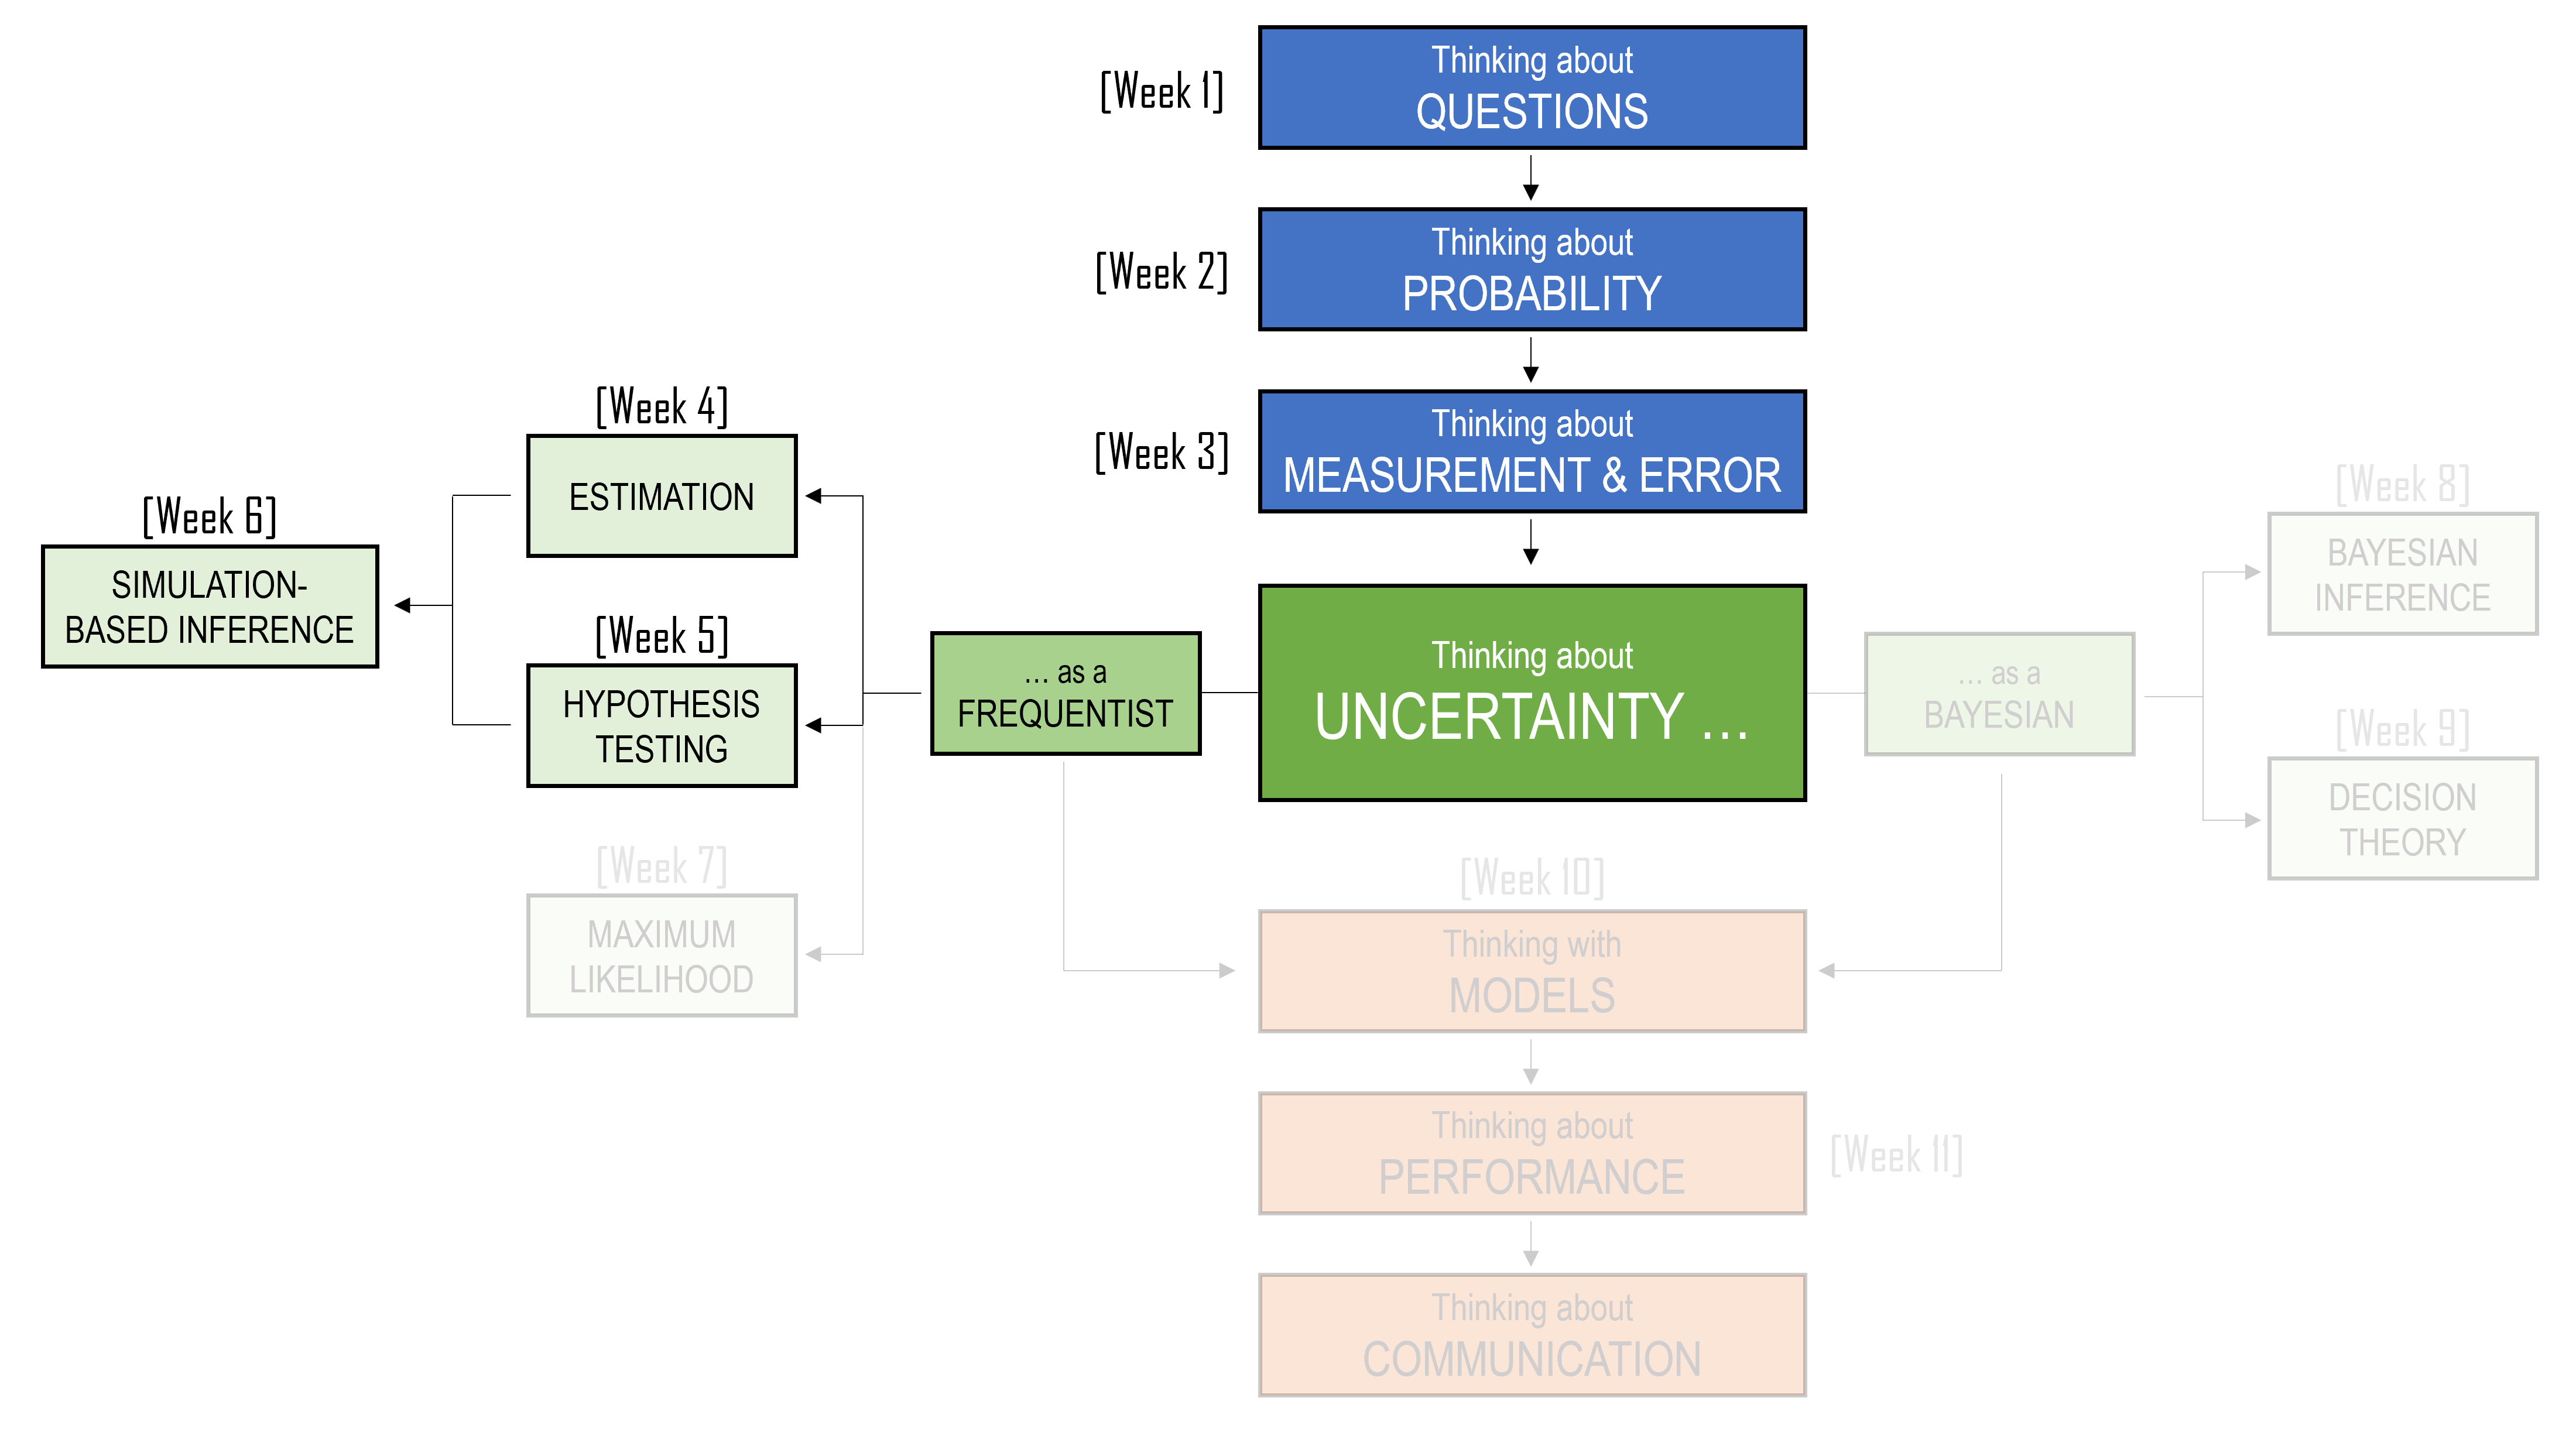
\includegraphics[width=14.81in,height=\textheight,keepaspectratio]{images/chapter6/outline.png}

\section{What does Solitaire and Nuclear Bombs have in
common?}\label{what-does-solitaire-and-nuclear-bombs-have-in-common}

On the morning of 16 July 1945, in the New Mexico desert, the United
States detonated the world's first nuclear weapon. The test was
code-named Trinity. The device itself was called the Gadget. It produced
an explosion equivalent to thousands of tonnes of TNT and marked the
culmination of the Manhattan Project: a vast, secret wartime effort that
brought together some of the most brilliant scientists and
mathematicians of the twentieth century.

Among them were J. Robert Oppenheimer, John von Neumann, and a
Polish-born mathematician named Stanisław Ulam. Ulam was not as publicly
famous as some of the others, but his mathematical imagination would
become central to a new way of solving problems. These problems involved
physical processes so complex that writing down an exact answer could be
close to impossible.

One of the great difficulties was understanding how neutrons move and
interact inside fissile material. The basic idea of a nuclear chain
reaction is simple enough to describe. A neutron strikes the nucleus of
an atom. The nucleus splits. Energy is released. More neutrons are
released. Those neutrons may then strike other nuclei, releasing still
more neutrons. If, on average, each stage produces enough further
reactions, the process grows rapidly.

But the details are much harder. A neutron might strike another nucleus.
It might scatter and change direction. It might slow down. It might
escape. It might be absorbed without producing another fission event.
Each possibility depends on features such as the neutron's position,
speed, energy, and the material around it.

\begin{figure}[H]

{\centering 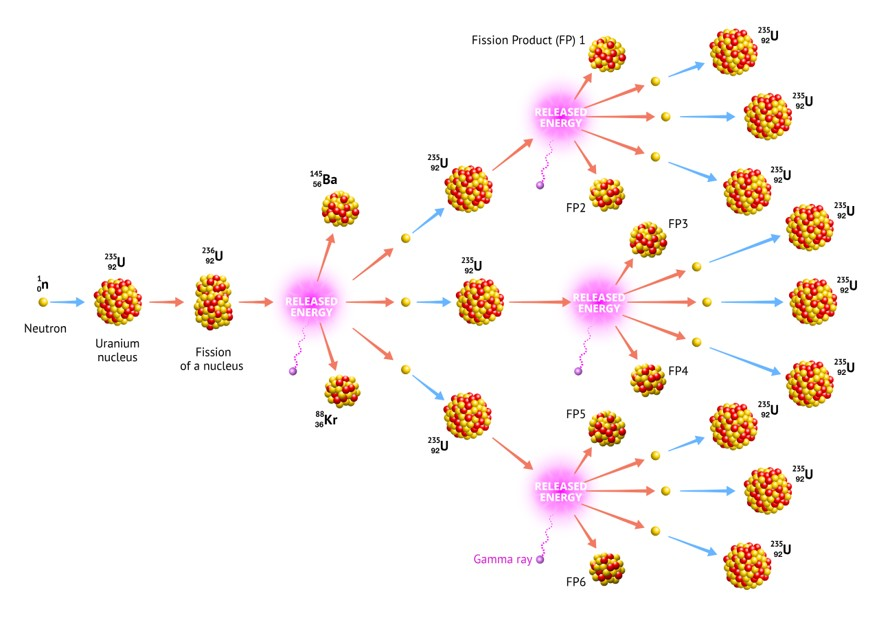
\includegraphics[width=2.93in,height=\textheight,keepaspectratio]{images/chapter6/chain-reaction.jpg}

}

\caption{Fission Chain Reaction. Image Source: Energy Encyclopedia}

\end{figure}%

So the question was not just:

\begin{quote}
What happens to one neutron?
\end{quote}

The question was closer to:

\begin{quote}
Across an enormous number of possible neutron histories, how often does
the process grow, fade out, or escape?
\end{quote}

Trying to calculate every possible path directly was hopeless. The
sample space was too large. There were too many branches, too many
dependencies, and too many possible histories.

Then, in early 1946, Ulam became seriously ill.~He developed
encephalitis, an inflammation of the brain, and nearly died. His
recovery was long and slow. Confined to bed, he passed the time by
playing solitaire. As he played, a question began to bother him:

\begin{quote}
What is the probability that a randomly shuffled game of solitaire can
be won?
\end{quote}

At first, this sounds like a straightforward probability question. In
principle, one could try to list all possible deals of the cards, work
out which deals lead to a win, and divide:

\[\frac{\text{number of winning deals}}{\text{number of possible deals}}\]

But in practice, this was a nightmare. The number of possible
arrangements of a deck of cards is enormous. The game also unfolds
through many decisions and dependencies. A neat formula was not easy to
find. A deck of 52 cards can be arranged in \(52!\) different ways. This
is approximately

\[8 \times10^{67}\]

That's 8 followed by 67 zeros.

That is an unimaginably large number of possible deals. Listing them all
was impossible. Analysing them all was impossible. Even describing the
full sample space in a useful way was practically impossible. But Ulam
noticed something. He did not need to list every possible game to learn
something about the probability of winning. He could play many games and
count the proportion that were won.

If he played 10 games, the answer would be rough. If he played 100
games, it might be better. If a machine could play thousands or millions
of games, the proportion of wins could become a useful approximation.
The idea was simple but powerful:

\begin{quote}
When the exact probability is too hard to calculate, simulate the random
process many times and count what happens.
\end{quote}

When Ulam returned to Los Alamos, the connection became clear. Solitaire
was only a card game, but the same way of thinking could be used for
much harder problems. Instead of trying to calculate every possible
neutron path exactly, one could simulate many possible neutron
histories. One simulated neutron might scatter. Another might escape.
Another might trigger a fission event and produce more neutrons, each
with its own possible path. Repeating this process again and again could
reveal the behaviour of the whole system.

This approach became known as the Monte Carlo method, named after the
casino district famous for games of chance. The name is playful, but the
idea is serious:

\begin{quote}
If we can imitate the random process often enough, we can learn what it
tends to do.
\end{quote}

In this chapter, we will use the same basic idea for statistical
inference.

\section{From formulae to simulation}\label{from-formulae-to-simulation}

In the previous chapter, we saw that many hypothesis tests follow the
same structure:

\begin{enumerate}
\def\labelenumi{\arabic{enumi}.}
\tightlist
\item
  State a benchmark claim.
\item
  Choose a statistic.
\item
  Work out what values of that statistic would be expected under the
  benchmark claim.
\item
  Compare the observed statistic with that reference distribution.
\end{enumerate}

The hard part is usually step 3. Sometimes probability theory gives us a
convenient answer. For example, when testing a mean, we may use a
\(t\)-distribution. When comparing proportions, we may use an
approximate normal distribution or a chi-squared test. These
formula-based methods are powerful and efficient.

But they are not the only way.

Suppose we want to know whether a statistic is unusual under some
assumption. If we can simulate many datasets under that assumption, then
we can calculate the statistic for each simulated dataset. This produces
an approximate sampling distribution.

Then we ask where the observed statistic sits in that simulated
distribution. This is the same logic as the p-value in Chapter 5. The
difference is how we get the reference distribution.

\begin{table}
\fontsize{12.0pt}{14.0pt}\selectfont
\begin{tabular*}{1\linewidth}{@{\extracolsep{\fill}}llll}
\toprule
Approach & How the reference distribution is obtained & Advantage & Risk \\ 
\midrule\addlinespace[2.5pt]
Formula-based & Use mathematical theory, such as the t distribution or normal approximation & Fast, exact or very accurate when assumptions hold & Can hide assumptions behind a formula \\ 
Simulation-based & Use a computer to create many hypothetical repeated results & Flexible and often easier to understand visually & Can be misleading if the simulation does not match the question \\ 
\bottomrule
\end{tabular*}
\end{table}

Simulation-based inference therefore does not replace statistical
thinking. It makes the thinking more visible. We must say exactly what
world we are simulating.

\section{Simulating from an assumed
model}\label{simulating-from-an-assumed-model}

Before we get to permutation tests and bootstrapping, it is useful to
see the basic idea of simulation in a simpler setting.

\begin{tcolorbox}[enhanced jigsaw, arc=.35mm, bottomrule=.15mm, bottomtitle=1mm, breakable, colback=white, colbacktitle=quarto-callout-note-color!10!white, colframe=quarto-callout-note-color-frame, coltitle=black, left=2mm, leftrule=.75mm, opacityback=0, opacitybacktitle=0.6, rightrule=.15mm, title=\textcolor{quarto-callout-note-color}{\faInfo}\hspace{0.5em}{A benchmark claim about household income}, titlerule=0mm, toprule=.15mm, toptitle=1mm]

Suppose we have a sample of 100 Australian households from an ABS-style
income survey. A benchmark claim is made:

\begin{quote}
The average annual household income in this population is \$100,000.
\end{quote}

In our sample, the mean household income is \$112,000.

Is a sample mean of \$112,000 surprisingly high if the true average
household income were \$100,000?

\end{tcolorbox}

Household income is usually right-skewed. Many households have incomes
near the middle of the distribution, while a smaller number of
households have very high incomes. A normal distribution may not
describe individual household incomes well.

For illustration, suppose we are willing to assume that household income
follows a log-normal distribution. A log-normal distribution is
right-skewed and only produces positive values, which makes it a simple
model for income-like data.

Under the benchmark claim, the mean household income is \$100,000. To
simulate realistic income values, we also need to assume a population
standard deviation. Suppose we use a standard deviation of \$70,000.

We can then simulate what the sample mean would look like if we
repeatedly sampled 100 households from a log-normal distribution with
mean \$100,000 and standard deviation \$70,000.

\begin{table}
\fontsize{12.0pt}{14.0pt}\selectfont
\begin{tabular*}{\linewidth}{@{\extracolsep{\fill}}rrrr}
\toprule
Number of simulations & Mean of simulated sample means & Observed sample mean & Simulated p-value \\ 
\midrule\addlinespace[2.5pt]
10000 & \$100,084 & \$112,000 & 0.051 \\ 
\bottomrule
\end{tabular*}
\end{table}

The simulated p-value is the proportion of simulated sample means that
were at least as large as \$112,000.

First, here is what the assumed lognormal model looks like at the level
of individual households. The individual incomes are clearly
right-skewed. Most households are clustered toward the lower and middle
part of the distribution, while a smaller number have much higher
incomes.

\pandocbounded{
\includegraphics[keepaspectratio]{6_SimulationBasedInference_files/figure-pdf/unnamed-chunk-6-1.pdf}}

Now here is the simulated distribution of sample means. Each value is an
average from a simulated sample of 100 households. Averaging reduces
some of the extreme variation, so the simulated sample means form a
distribution that is more concentrated and more bell-shaped. This is the
Central Limit Theorem appearing through simulation rather than through a
formula.

\pandocbounded{
\includegraphics[keepaspectratio]{6_SimulationBasedInference_files/figure-pdf/unnamed-chunk-7-1.pdf}}

But this approach relies on strong assumptions. We had to assume not
only that the true mean was \$100,000, but also that household incomes
followed a log-normal distribution with a standard deviation of
\$70,000.In many practical settings, we do not want to make such a
specific distributional assumption.

Permutation tests offer another route.

\section{Permutation tests}\label{permutation-tests}

A permutation test is a simulation-based hypothesis test built around
the idea of \textbf{shuffling}. The basic logic is:

\begin{quote}
If the explanatory variable is unrelated to the outcome, then the labels
attached to the observations could have been arranged differently.
\end{quote}

This is easier to understand with data. We will return to the household
income example from Chapters 4 and 5.

\begin{tcolorbox}[enhanced jigsaw, arc=.35mm, bottomrule=.15mm, bottomtitle=1mm, breakable, colback=white, colbacktitle=quarto-callout-note-color!10!white, colframe=quarto-callout-note-color-frame, coltitle=black, left=2mm, leftrule=.75mm, opacityback=0, opacitybacktitle=0.6, rightrule=.15mm, title=\textcolor{quarto-callout-note-color}{\faInfo}\hspace{0.5em}{Household income in capital city and regional areas}, titlerule=0mm, toprule=.15mm, toptitle=1mm]

Suppose we collect annual household income data from two groups:

\begin{itemize}
\tightlist
\item
  households in capital city areas;
\item
  households in regional areas.
\end{itemize}

We want to know whether household income is associated with region.

\end{tcolorbox}

In Chapter 4, this was an estimation question:

\begin{quote}
How large is the difference between mean household incomes in the two
groups?
\end{quote}

In Chapter 5, this became a hypothesis testing question:

\begin{quote}
Is the observed difference surprising if the two population means are
equal?
\end{quote}

Now we will answer the testing question by simulation. Let us use the
same type of illustrative income data as before. The data are simulated
for teaching purposes, but the context is the same: an ABS-style
household income survey.

\begin{table}
\fontsize{12.0pt}{14.0pt}\selectfont
\begin{tabular*}{\linewidth}{@{\extracolsep{\fill}}lrrrr}
\toprule
region & n & Sample mean & Sample median & Sample standard deviation \\ 
\midrule\addlinespace[2.5pt]
Capital city & 80 & \$104,609 & \$93,100 & \$58,395 \\ 
Regional & 80 & \$84,649 & \$77,350 & \$43,412 \\ 
\bottomrule
\end{tabular*}
\end{table}

The two groups have different sample means. Let us calculate the
observed difference as:

\[\bar{x}_{\text{capital}} - \bar{x}_{\text{regional}}= \text{19,960}\]

The key question is not whether the sample means are exactly equal. They
almost certainly will not be exactly equal. The key question is:

\begin{quote}
Would a difference this large be surprising if region were not
associated with income?
\end{quote}

This is where the permutation test begins.

\subsection{The shuffling idea}\label{the-shuffling-idea}

Suppose the region labels do not matter. That is, suppose income is not
associated with whether a household is labelled ``Capital city'' or
``Regional''.

Under this benchmark claim, the incomes are still the incomes. We do not
change them. The observed incomes are part of the data. What changes is
the labels.

If region does not matter, then the label ``Capital city'' could have
been attached to a different set of 80 households, and the label
``Regional'' could have been attached to the remaining 80 households.

So we shuffle the region labels. Each shuffle gives one possible world
where region is unrelated to income. For each shuffled world, we
calculate the difference in mean incomes between the two shuffled
groups.

\begin{table}
\fontsize{12.0pt}{14.0pt}\selectfont
\begin{tabular*}{\linewidth}{@{\extracolsep{\fill}}cccc}
\toprule
id & income & Original label & Shuffled label \\ 
\midrule\addlinespace[2.5pt]
1 & \$113,100 & Capital city & Regional \\ 
2 & \$117,200 & Regional & Regional \\ 
3 & \$253,200 & Capital city & Capital city \\ 
4 & \$143,541 & Regional & Capital city \\ 
5 & \$118,152 & Capital city & Regional \\ 
... & ... & ... & ... \\ 
160 & \$157,214 & Regional & Capital city \\ 
\bottomrule
\end{tabular*}
\end{table}

Next, the sample statistics are computed for the date grouped by the
shuffled labels. Then we repeat the process many times.

\begin{table}
\fontsize{12.0pt}{14.0pt}\selectfont
\begin{tabular*}{\linewidth}{@{\extracolsep{\fill}}lrrr}
\toprule
shuffle & Capital city mean & Regional mean & Capital minus regional \\ 
\midrule\addlinespace[2.5pt]
Observed data & \$104,609 & \$84,649 & \$19,960 \\ 
Shuffle 1 & \$86,076 & \$103,181 & -\$17,105 \\ 
Shuffle 2 & \$92,380 & \$96,878 & -\$4,498 \\ 
Shuffle 3 & \$98,681 & \$90,576 & \$8,105 \\ 
Shuffle 4 & \$98,070 & \$91,188 & \$6,882 \\ 
Shuffle 5 & \$97,041 & \$92,216 & \$4,825 \\ 
Shuffle 6 & \$97,904 & \$91,354 & \$6,550 \\ 
Shuffle 7 & \$92,931 & \$96,326 & -\$3,395 \\ 
Shuffle 8 & \$93,760 & \$95,498 & -\$1,738 \\ 
\bottomrule
\end{tabular*}
\end{table}

\subsection{A permutation test for the difference in
means}\label{a-permutation-test-for-the-difference-in-means}

Suppose we did this shuffling process 5000 times. The summary statistics
are provided below.

\begin{table}
\fontsize{12.0pt}{14.0pt}\selectfont
\begin{tabular*}{\linewidth}{@{\extracolsep{\fill}}rrrrr}
\toprule
Number of permutations & Mean of permuted differences & Standard deviation of permuted differences & Smallest permuted difference & Largest permuted difference \\ 
\midrule\addlinespace[2.5pt]
5000 & -\$43 & \$8,241 & -\$29,495 & \$28,448 \\ 
\bottomrule
\end{tabular*}
\end{table}

The simulated differences are centred close to zero. This is exactly
what we should expect. If region labels do not matter, then sometimes
the shuffled capital city group will have a higher mean, sometimes the
shuffled regional group will have a higher mean, and the long-run centre
should be near zero.

\pandocbounded{
\includegraphics[keepaspectratio]{6_SimulationBasedInference_files/figure-pdf/unnamed-chunk-14-1.pdf}}

The histogram is the simulated null distribution. It shows what
differences in mean income would look like if region were not associated
with income. The solid vertical line is the observed difference. If the
observed difference is far out in the tail of the histogram, then it is
difficult to explain by shuffled labels alone.

\subsection{The simulated p-value}\label{the-simulated-p-value}

A p-value is a tail proportion. In a simulation-based test, it is
estimated by counting how many simulated statistics are at least as
extreme as the observed statistic.

\pandocbounded{
\includegraphics[keepaspectratio]{6_SimulationBasedInference_files/figure-pdf/unnamed-chunk-15-1.pdf}}

For a two-sided test, we count simulated differences whose absolute
value is at least as large as the absolute value of the observed
difference:

\[\text{simulated p-value}
=
\frac{\text{number of simulated } |D| \ge |D_{\text{obs}}|}{\text{number of simulations}}.\]

\begin{table}
\fontsize{12.0pt}{14.0pt}\selectfont
\begin{tabular*}{1\linewidth}{@{\extracolsep{\fill}}llr}
\toprule
Test & Tail rule & Simulated p-value \\ 
\midrule\addlinespace[2.5pt]
One-sided: capital city mean is higher & Count permuted differences >= observed difference & 0.0084 \\ 
Two-sided: means differ & Count |permuted difference| >= |observed difference| & 0.0158 \\ 
\bottomrule
\end{tabular*}
\end{table}

The p-value is not the probability that the two regions have the same
population mean. It is the proportion of simulated shuffled worlds that
produced a difference at least as extreme as the one we observed.

A small p-value says:

\begin{quote}
Differences this large were rare in the shuffled worlds.
\end{quote}

It does not say:

\begin{quote}
The null hypothesis has this probability of being true.
\end{quote}

That warning is the same as in Chapter 5. Simulation changes the
calculation, not the interpretation.

\subsection{What a permutation test
preserves}\label{what-a-permutation-test-preserves}

A permutation test is powerful because it keeps some features of the
data exactly as they were observed.

In the income example, the permutation test preserves:

\begin{itemize}
\tightlist
\item
  the full set of observed incomes;
\item
  the number of capital city labels;
\item
  the number of regional labels;
\item
  the skewness and outliers in the income distribution.
\end{itemize}

But it breaks the connection between income and region.

\begin{table}
\fontsize{12.0pt}{14.0pt}\selectfont
\begin{tabular*}{1\linewidth}{@{\extracolsep{\fill}}ll}
\toprule
Feature of the data & What happens in a permutation test? \\ 
\midrule\addlinespace[2.5pt]
The observed income values & Preserved \\ 
The number of households in each group & Preserved \\ 
The association between income and region & Broken by shuffling labels \\ 
The shape of the income distribution & Preserved \\ 
\bottomrule
\end{tabular*}
\end{table}

This makes the permutation test a natural method for testing whether two
variables are associated. It creates a world where the association has
been removed, while leaving the observed values themselves intact.

\begin{tcolorbox}[enhanced jigsaw, arc=.35mm, bottomrule=.15mm, bottomtitle=1mm, breakable, colback=white, colbacktitle=quarto-callout-important-color!10!white, colframe=quarto-callout-important-color-frame, coltitle=black, left=2mm, leftrule=.75mm, opacityback=0, opacitybacktitle=0.6, rightrule=.15mm, title=\textcolor{quarto-callout-important-color}{\faExclamation}\hspace{0.5em}{The key question for a permutation test}, titlerule=0mm, toprule=.15mm, toptitle=1mm]

A permutation test asks:

\begin{quote}
What would our statistic look like if the labels were exchangeable?
\end{quote}

In the income example, this means asking what differences in mean income
would look like if the labels ``Capital city'' and ``Regional'' could be
shuffled among the households without changing anything important.

\end{tcolorbox}

\subsection{When is a permutation test
reasonable?}\label{when-is-a-permutation-test-reasonable}

The shuffling idea depends on a condition called
\textbf{exchangeability}. Roughly, observations are exchangeable under
the benchmark claim if rearranging the labels would be consistent with
that claim.

For a two-group comparison, this means that if the benchmark claim is
true, the group labels should not carry information about the outcome.

This is especially natural in a randomised experiment. Suppose people
are randomly assigned to two teaching methods. If the teaching method
has no effect, then the labels ``Method A'' and ``Method B'' are
exchangeable. We could shuffle them and create another possible random
assignment.

For observational data, such as household income by region, the idea
requires more care. Households are not randomly assigned to live in
capital city or regional areas. Region may be connected to employment
opportunities, industry, housing costs, household composition,
education, and many other factors. A permutation test can still answer a
precise question about the observed data, but we should be cautious
about turning that answer into a causal story.

In this chapter, our question is not:

\begin{quote}
Does living in a capital city cause a household to have a higher income?
\end{quote}

The safer question is:

\begin{quote}
Is the observed association between region and income larger than we
would expect from randomly shuffled region labels?
\end{quote}

That distinction matters.

\section{Bootstrap methods}\label{bootstrap-methods}

In Chapter 4, we learned that the uncertainty in an estimate is about
what would happen across repeated samples. But in real life, we usually
have only one sample. The ABS does not repeatedly draw thousands of new
samples just so we can see how our estimate changes. So what can we do?

The bootstrap uses a clever approximation:

\begin{quote}
If the sample is a reasonable miniature version of the population, then
resampling from the sample can mimic repeated sampling from the
population.
\end{quote}

The word bootstrap comes from the expression ``to pull oneself up by
one's bootstraps''.

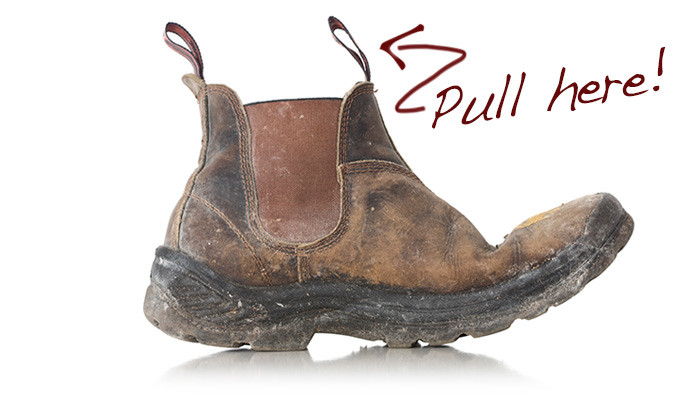
\includegraphics[width=2.33in,height=\textheight,keepaspectratio]{images/chapter6/bootstrap.jpg}

The statistical bootstrap has the same flavour. We use the sample itself
to learn about the uncertainty in a statistic calculated from that
sample. The key operation is \textbf{sampling with replacement}.

Suppose our sample contains five incomes:

\[52000,\ 61000,\ 68000,\ 73000,\ 420000.\]

A bootstrap sample of size five is created by randomly choosing five
values from this list, replacing each value after it is chosen. This
means the same value can appear more than once, and some original values
may not appear at all.

\begin{table}
\fontsize{12.0pt}{14.0pt}\selectfont
\begin{tabular*}{\linewidth}{@{\extracolsep{\fill}}rrrr}
\toprule
Original sample & Bootstrap sample 1 & Bootstrap sample 2 & Bootstrap sample 3 \\ 
\midrule\addlinespace[2.5pt]
\$52,000 & \$52,000 & \$52,000 & \$68,000 \\ 
\$61,000 & \$68,000 & \$73,000 & \$68,000 \\ 
\$68,000 & \$73,000 & \$68,000 & \$420,000 \\ 
\$73,000 & \$61,000 & \$61,000 & \$61,000 \\ 
\$420,000 & \$420,000 & \$420,000 & \$61,000 \\ 
\bottomrule
\end{tabular*}
\end{table}

Each bootstrap sample is the same size as the original sample, but it is
not the same set of values. Some values repeat. Others disappear. This
repetition and disappearance is what creates variation across bootstrap
samples.

\begin{tcolorbox}[enhanced jigsaw, arc=.35mm, bottomrule=.15mm, bottomtitle=1mm, breakable, colback=white, colbacktitle=quarto-callout-important-color!10!white, colframe=quarto-callout-important-color-frame, coltitle=black, left=2mm, leftrule=.75mm, opacityback=0, opacitybacktitle=0.6, rightrule=.15mm, title=\textcolor{quarto-callout-important-color}{\faExclamation}\hspace{0.5em}{Note: Bootstrap samples are not permutations}, titlerule=0mm, toprule=.15mm, toptitle=1mm]

A permutation rearranges the existing observations without changing how
many times each one appears.

A bootstrap sample resamples with replacement, so some observations can
appear more than once and others can be absent.

\end{tcolorbox}

\subsection{Bootstrapping the mean income in one
sample}\label{bootstrapping-the-mean-income-in-one-sample}

Let us first bootstrap the mean household income for all households in
our illustrative dataset, ignoring region.

Suppose the sample mean for our 160 households is \$94,629.

\begin{verbatim}
[1] 94628.75
\end{verbatim}

To bootstrap this estimate:

\begin{enumerate}
\def\labelenumi{\arabic{enumi}.}
\tightlist
\item
  Resample 160 households from the observed 160 households, with
  replacement.
\item
  Calculate the mean income in the bootstrap sample.
\item
  Repeat many times.
\item
  Examine the distribution of bootstrap means.
\end{enumerate}

Suppose the table below represents 5000 bootstap samples for our data.

\begin{table}
\fontsize{12.0pt}{14.0pt}\selectfont
\begin{tabular*}{\linewidth}{@{\extracolsep{\fill}}rr}
\toprule
simulation & mean\_income \\ 
\midrule\addlinespace[2.5pt]
1 & \$94,306 \\ 
2 & \$93,706 \\ 
3 & \$90,163 \\ 
4 & \$95,591 \\ 
5 & \$90,667 \\ 
... & ... \\ 
4996 & \$100,671 \\ 
4997 & \$103,218 \\ 
4998 & \$92,954 \\ 
4999 & \$101,773 \\ 
5000 & \$93,399 \\ 
\bottomrule
\end{tabular*}
\end{table}

And the following table provides summary statistics for our boostrap
sample:

\begin{table}
\fontsize{12.0pt}{14.0pt}\selectfont
\begin{tabular*}{\linewidth}{@{\extracolsep{\fill}}rrrrr}
\toprule
Observed mean & Mean of bootstrap means & Bootstrap standard error & 2.5th percentile & 97.5th percentile \\ 
\midrule\addlinespace[2.5pt]
\$94,629 & \$94,657 & \$4,222 & \$86,668 & \$103,296 \\ 
\bottomrule
\end{tabular*}
\end{table}

The bootstrap standard error is the standard deviation of the bootstrap
estimates. It estimates how much the sample mean might vary from sample
to sample.

The interval from the 2.5th percentile to the 97.5th percentile is
called a \textbf{percentile bootstrap confidence interval}.

\pandocbounded{
\includegraphics[keepaspectratio]{6_SimulationBasedInference_files/figure-pdf/unnamed-chunk-23-1.pdf}}

The histogram shows the bootstrap distribution of the mean. It is not a
distribution of individual incomes. It is a distribution of estimates.

This distinction is central:

\begin{itemize}
\tightlist
\item
  The original income distribution shows variation between households.
\item
  The bootstrap distribution shows variation between possible estimates.
\end{itemize}

\subsection{The percentile bootstrap confidence
interval}\label{the-percentile-bootstrap-confidence-interval}

The percentile bootstrap interval is simple to construct.

For an approximate 95\% confidence interval:

\begin{enumerate}
\def\labelenumi{\arabic{enumi}.}
\tightlist
\item
  Generate many bootstrap samples.
\item
  Calculate the statistic of interest for each bootstrap sample.
\item
  Sort the bootstrap statistics.
\item
  Use the 2.5th and 97.5th percentiles as the interval endpoints.
\end{enumerate}

The idea is that the middle 95\% of the bootstrap estimates gives a
plausible range for the population parameter.

In notation, if the bootstrap estimates are:

\[\hat{\theta}^{[1]},\ \hat{\theta}^{[2]},\ \ldots,\ \hat{\theta}^{[B]},\]

then the percentile bootstrap interval is:

\[\left(
\hat{\theta}^{[0.025]},
\hat{\theta}^{[0.975]}
\right),\]

where these represent the 2.5th and 97.5th percentiles of the bootstrap
estimates. This method is popular because it is easy to explain and easy
to implement. It also works for many statistics where a standard formula
is awkward.

\subsection{Bootstrapping the median}\label{bootstrapping-the-median}

The median is an important example. Income data are often skewed, and
the median is often more meaningful than the mean when describing a
typical household.

But the standard error of the median is less familiar than the standard
error of the mean. In an introductory course, we may not have a
convenient formula for it. The bootstrap gives us a practical solution.

\begin{table}
\fontsize{12.0pt}{14.0pt}\selectfont
\begin{tabular*}{\linewidth}{@{\extracolsep{\fill}}rrrr}
\toprule
Observed median & Bootstrap standard error & 2.5th percentile & 97.5th percentile \\ 
\midrule\addlinespace[2.5pt]
\$85,150 & \$4,515 & \$76,400 & \$93,800 \\ 
\bottomrule
\end{tabular*}
\end{table}

\pandocbounded{
\includegraphics[keepaspectratio]{6_SimulationBasedInference_files/figure-pdf/unnamed-chunk-26-1.pdf}}

Notice that the bootstrap distribution for the median may look less
smooth than the bootstrap distribution for the mean. This happens
because the median can only take certain values from the data,
especially when the sample size is not very large.

This is a useful reminder:

\begin{quote}
The bootstrap is flexible, but it is still built from the data we have.
\end{quote}

If the sample is small, or if the statistic depends heavily on a few
observations, the bootstrap distribution may be rough.

\subsection{Bootstrap confidence interval for a difference in
means}\label{bootstrap-confidence-interval-for-a-difference-in-means}

Let us now return to the comparison between capital city and regional
households. In Chapter 5, we tested whether the difference in mean
incomes was larger than expected under a benchmark claim. Here we
estimate the uncertainty in the size of that difference. The parameter
of interest is:

\[\mu_{\text{capital}} - \mu_{\text{regional}}\]

The estimate is:

\[\bar{x}_{\text{capital}} - \bar{x}_{\text{regional}}\]

For independent groups, the bootstrap should re-sample within each group
separately. This preserves the two-sample structure.

\begin{table}
\fontsize{12.0pt}{14.0pt}\selectfont
\begin{tabular*}{\linewidth}{@{\extracolsep{\fill}}rrrr}
\toprule
Observed difference & Bootstrap standard error & 2.5th percentile & 97.5th percentile \\ 
\midrule\addlinespace[2.5pt]
\$19,960 & \$7,996 & \$5,024 & \$36,022 \\ 
\bottomrule
\end{tabular*}
\end{table}

\pandocbounded{
\includegraphics[keepaspectratio]{6_SimulationBasedInference_files/figure-pdf/unnamed-chunk-29-1.pdf}}

The dotted vertical line marks zero. If the interval is entirely above
zero, then the bootstrap interval suggests that positive differences are
the plausible values. But remember the role of the bootstrap here: it is
estimating uncertainty in the size of the difference. It is not
primarily constructing a null distribution.

This is why the bootstrap distribution is centred near the observed
difference, while the permutation distribution was centred near zero.

\pandocbounded{
\includegraphics[keepaspectratio]{6_SimulationBasedInference_files/figure-pdf/unnamed-chunk-30-1.pdf}}

The \textbf{permutation distribution} is centred near zero because it
represents a world where region labels do not matter.

The \textbf{bootstrap distribution} is centred near the observed
estimate because it represents repeated sampling from a population that
looks like the observed sample.

So the two distributions have different centres because they answer
different questions.

\begin{table}
\fontsize{12.0pt}{14.0pt}\selectfont
\begin{tabular*}{1\linewidth}{@{\extracolsep{\fill}}llll}
\toprule
Distribution & Centred near & Why? & Used mainly for \\ 
\midrule\addlinespace[2.5pt]
Permutation & The benchmark value, often 0 & It simulates a world where the null claim is true & p-values \\ 
Bootstrap & The observed estimate & It simulates repeated samples from a population like the observed sample & standard errors and confidence intervals \\ 
\bottomrule
\end{tabular*}
\end{table}

\subsection{Paired data and the
bootstrap}\label{paired-data-and-the-bootstrap}

The bootstrap can also be used for paired data. Suppose we observe the
same households under two measurements, such as income before and after
housing costs. Since both values come from the same household, the two
values are paired. In a paired problem, we should not re-sample the
before values separately from the after values. That would break the
pairing.

Instead, we first calculate the within-household differences:

\[D_i = X_i - Y_i\]

Then we bootstrap the differences.

\begin{table}
\fontsize{12.0pt}{14.0pt}\selectfont
\begin{tabular*}{\linewidth}{@{\extracolsep{\fill}}rrrr}
\toprule
n & Mean before housing costs & Mean after housing costs & Mean difference \\ 
\midrule\addlinespace[2.5pt]
60 & \$93,355 & \$68,390 & \$24,965 \\ 
\bottomrule
\end{tabular*}
\end{table}

\begin{table}
\fontsize{12.0pt}{14.0pt}\selectfont
\begin{tabular*}{\linewidth}{@{\extracolsep{\fill}}rrrr}
\toprule
Observed mean difference & Bootstrap standard error & 2.5th percentile & 97.5th percentile \\ 
\midrule\addlinespace[2.5pt]
\$24,965 & \$863 & \$23,270 & \$26,657 \\ 
\bottomrule
\end{tabular*}
\end{table}

The important point is not the particular numbers. The important point
is the structure. With paired data, resample the pairs or resample the
differences. Do not break the pairing.

\subsection{When the bootstrap works well, and when it can
struggle}\label{when-the-bootstrap-works-well-and-when-it-can-struggle}

The bootstrap is a remarkably useful method, but it is not a guarantee
of truth. The bootstrap treats the sample as a stand-in for the
population. This is reasonable when the sample is large enough and
representative enough to capture the important features of the
population. But the bootstrap can struggle when:

\begin{itemize}
\tightlist
\item
  the sample size is very small
\item
  the sample misses important parts of the population
\item
  the statistic depends on extreme values
\item
  the population has rare but important tail behaviour
\item
  the data are biased or poorly measured
\end{itemize}

For example, suppose the true population contains a small number of
extremely high-income households, but none of them appear in our sample.
The bootstrap cannot invent the missing high-income households. It can
only resample from what was observed.

it is important to remember that:

\begin{quote}
The bootstrap cannot fix a bad sample.
\end{quote}

It can describe the uncertainty implied by the data we have. It cannot
repair data that were collected from the wrong population, measured
badly, or missing important values. A useful habit is to always plot the
bootstrap distribution. If it is extremely rough, heavily skewed, or
dominated by a few repeated observations, then the bootstrap interval
should be interpreted cautiously.

\section{Optional extension: Can the bootstrap be used for hypothesis
testing?}\label{optional-extension-can-the-bootstrap-be-used-for-hypothesis-testing}

So far, we have used permutation tests for hypothesis testing and
bootstrap methods for confidence intervals. This is the cleanest
distinction:

\begin{itemize}
\tightlist
\item
  permutation tests simulate what would happen if the group labels did
  not matter;
\item
  bootstrap methods simulate how much an estimate might vary from sample
  to sample.
\end{itemize}

However, the bootstrap can also be adapted for hypothesis testing. The
main complication is that, for a test, we need to simulate from a world
where the benchmark claim is true. Suppose we are comparing mean
household income in capital city and regional areas. The observed
difference is:

\[\bar{x}_{\text{capital}} - \bar{x}_{\text{regional}}\]

If we simply bootstrap from the original capital city and regional
samples, we simulate a world that looks like the data we observed. But
that world may already contain a real difference between the groups.
That is useful for a confidence interval, but it is not the right
reference world for a hypothesis test.

For a hypothesis test, we need to simulate a world where the population
mean difference is zero.

One simple method is to \textbf{recentre} the data.

\begin{enumerate}
\def\labelenumi{\arabic{enumi}.}
\tightlist
\item
  Compute the mean income in each group.
\item
  Compute the overall mean income.
\item
  Shift the capital city incomes so their mean becomes the overall mean.
\item
  Shift the regional incomes so their mean also becomes the overall
  mean.
\item
  Bootstrap from these shifted samples.
\item
  Calculate the difference in means for each bootstrap sample.
\item
  Compare the observed difference with this bootstrap null distribution.
\end{enumerate}

\begin{Shaded}
\begin{Highlighting}[]
\NormalTok{overall\_mean }\OtherTok{\textless{}{-}} \FunctionTok{mean}\NormalTok{(income\_regions}\SpecialCharTok{$}\NormalTok{income)}
\NormalTok{capital\_mean }\OtherTok{\textless{}{-}} \FunctionTok{mean}\NormalTok{(capital\_income)}
\NormalTok{regional\_mean }\OtherTok{\textless{}{-}} \FunctionTok{mean}\NormalTok{(regional\_income)}

\NormalTok{capital\_shifted }\OtherTok{\textless{}{-}}\NormalTok{ capital\_income }\SpecialCharTok{{-}}\NormalTok{ capital\_mean }\SpecialCharTok{+}\NormalTok{ overall\_mean}
\NormalTok{regional\_shifted }\OtherTok{\textless{}{-}}\NormalTok{ regional\_income }\SpecialCharTok{{-}}\NormalTok{ regional\_mean }\SpecialCharTok{+}\NormalTok{ overall\_mean}

\FunctionTok{mean}\NormalTok{(capital\_shifted)}
\end{Highlighting}
\end{Shaded}

\begin{verbatim}
[1] 94628.75
\end{verbatim}

\begin{Shaded}
\begin{Highlighting}[]
\FunctionTok{mean}\NormalTok{(regional\_shifted)}
\end{Highlighting}
\end{Shaded}

\begin{verbatim}
[1] 94628.75
\end{verbatim}

Both shifted groups now have the same mean. We have created a modified
version of the data where the benchmark claim is true.

Now we bootstrap from the shifted groups.

\begin{Shaded}
\begin{Highlighting}[]
\FunctionTok{set.seed}\NormalTok{(}\DecValTok{2420}\NormalTok{)}

\NormalTok{boot\_null\_diffs }\OtherTok{\textless{}{-}} \FunctionTok{tibble}\NormalTok{(}
  \AttributeTok{simulation =} \DecValTok{1}\SpecialCharTok{:}\NormalTok{B,}
  \AttributeTok{diff =} \FunctionTok{replicate}\NormalTok{(B, \{}
\NormalTok{    boot\_capital }\OtherTok{\textless{}{-}} \FunctionTok{sample}\NormalTok{(capital\_shifted, }\AttributeTok{size =} \FunctionTok{length}\NormalTok{(capital\_shifted), }\AttributeTok{replace =} \ConstantTok{TRUE}\NormalTok{)}
\NormalTok{    boot\_regional }\OtherTok{\textless{}{-}} \FunctionTok{sample}\NormalTok{(regional\_shifted, }\AttributeTok{size =} \FunctionTok{length}\NormalTok{(regional\_shifted), }\AttributeTok{replace =} \ConstantTok{TRUE}\NormalTok{)}
    \FunctionTok{mean}\NormalTok{(boot\_capital) }\SpecialCharTok{{-}} \FunctionTok{mean}\NormalTok{(boot\_regional)}
\NormalTok{  \})}
\NormalTok{)}

\NormalTok{boot\_test\_p }\OtherTok{\textless{}{-}} \FunctionTok{mean}\NormalTok{(}\FunctionTok{abs}\NormalTok{(boot\_null\_diffs}\SpecialCharTok{$}\NormalTok{diff) }\SpecialCharTok{\textgreater{}=} \FunctionTok{abs}\NormalTok{(observed\_diff))}
\end{Highlighting}
\end{Shaded}

\pandocbounded{
\includegraphics[keepaspectratio]{6_SimulationBasedInference_files/figure-pdf/unnamed-chunk-37-1.pdf}}

\begin{table}
\fontsize{12.0pt}{14.0pt}\selectfont
\begin{tabular*}{\linewidth}{@{\extracolsep{\fill}}lr}
\toprule
Method & Two-sided simulated p-value \\ 
\midrule\addlinespace[2.5pt]
Permutation test & 0.0158 \\ 
Bootstrap test after recentring & 0.0130 \\ 
\bottomrule
\end{tabular*}
\end{table}

This produces a bootstrap version of a null distribution.

The reason we do not use this as the main testing method is that it is
less transparent than a permutation test. In a permutation test, the
benchmark claim says the labels do not matter, so we shuffle the labels.
In a bootstrap test, we first have to construct a modified version of
the data where the benchmark claim is true. That extra step is powerful,
but it is also easier to misunderstand.

For this reason, in this unit we use:

\begin{itemize}
\tightlist
\item
  permutation tests for simulation-based hypothesis testing;
\item
  bootstrap methods for simulation-based confidence intervals.
\end{itemize}

The bootstrap test is useful to know about, but it is not the main
method we rely on here.

\section{Summary}\label{summary}

Simulation-based inference uses repeated computation to understand what
kinds of statistics we might expect under a particular process.

Permutation tests simulate a world where the labels are exchangeable.
They are mainly used for hypothesis testing. In the household income
example, we shuffled the region labels to ask whether the observed
difference between capital city and regional incomes was unusual under a
benchmark world where region did not matter.

Bootstrap methods simulate repeated sampling from a population that
looks like the observed sample. They are mainly used for estimating
uncertainty. In the household income example, we resampled households
with replacement to estimate the sampling variability of means, medians,
and differences between groups.

\begin{table}
\fontsize{12.0pt}{14.0pt}\selectfont
\begin{tabular*}{1\linewidth}{@{\extracolsep{\fill}}lll}
\toprule
Feature & Permutation test & Bootstrap \\ 
\midrule\addlinespace[2.5pt]
Main question & What would happen if the labels did not matter? & How much might the estimate vary from sample to sample? \\ 
What is resampled? & Labels are shuffled among observations & Observations are resampled from the sample \\ 
Replacement? & No; labels are rearranged & Yes; observations can repeat \\ 
Typical centre of simulated distribution & The benchmark value, often 0 & The observed estimate \\ 
Common output & Simulated p-value & Standard error or confidence interval \\ 
\bottomrule
\end{tabular*}
\end{table}

The computer can repeat an analysis thousands of times. But the computer
does not know what question we are asking. That remains our job.

\section{Exercises}\label{exercises-5}

\begin{tcolorbox}[enhanced jigsaw, arc=.35mm, bottomrule=.15mm, bottomtitle=1mm, breakable, colback=white, colbacktitle=quarto-callout-note-color!10!white, colframe=quarto-callout-note-color-frame, coltitle=black, left=2mm, leftrule=.75mm, opacityback=0, opacitybacktitle=0.6, rightrule=.15mm, title=\textcolor{quarto-callout-note-color}{\faInfo}\hspace{0.5em}{Question 1}, titlerule=0mm, toprule=.15mm, toptitle=1mm]

A cafe owner wants to know whether customers spend more when they order
through a mobile app than when they order at the counter. The owner
collects the following sample of order amounts, in dollars.

\begin{table}
\fontsize{12.0pt}{14.0pt}\selectfont
\begin{tabular*}{\linewidth}{@{\extracolsep{\fill}}lrrr}
\toprule
Method & n & Mean amount & Median amount \\ 
\midrule\addlinespace[2.5pt]
Counter & 12 & \$18.75 & \$18.50 \\ 
Mobile app & 12 & \$24.17 & \$24.50 \\ 
\bottomrule
\end{tabular*}
\end{table}

\begin{enumerate}
\def\labelenumi{(\alph{enumi})}
\tightlist
\item
  What is the observed difference in mean order amount, using:
\end{enumerate}

\[\bar{x}_{\text{app}} - \bar{x}_{\text{counter}}?\]

\begin{enumerate}
\def\labelenumi{(\alph{enumi})}
\setcounter{enumi}{1}
\item
  Explain how you would conduct a permutation test for this difference.
\item
  In the context of this example, what does it mean to shuffle the
  labels?
\item
  Suppose a permutation test gives a two-sided p-value of 0.018.
  Interpret this p-value in context.
\end{enumerate}

\begin{quote}
\textbf{Click for Solutions}

\begin{enumerate}
\def\labelenumi{(\alph{enumi})}
\tightlist
\item
  The mobile app mean is:
\end{enumerate}

\[\frac{18+22+\cdots+29}{12} = 24.17\]

The counter mean is:

\[\frac{15+18+\cdots+19}{12} = 18.75\]

So the observed difference is:

\[24.17 - 18.75 = 5.42\]

The mobile app orders are higher by about \$5.42 in this sample.

\begin{enumerate}
\def\labelenumi{(\alph{enumi})}
\setcounter{enumi}{1}
\tightlist
\item
  To conduct a permutation test:
\end{enumerate}

\begin{enumerate}
\def\labelenumi{\arabic{enumi}.}
\tightlist
\item
  Keep all 24 order amounts fixed.
\item
  Shuffle the labels ``Mobile app'' and ``Counter'' among the 24 orders.
\item
  Calculate the difference in mean order amount for the shuffled data.
\item
  Repeat many times.
\item
  Compare the observed difference of 5.42 with the shuffled differences.
\end{enumerate}

\begin{enumerate}
\def\labelenumi{(\alph{enumi})}
\setcounter{enumi}{2}
\item
  Shuffling the labels means pretending that the ordering method does
  not matter. The order amounts stay the same, but the labels ``Mobile
  app'' and ``Counter'' are randomly reassigned to the orders.
\item
  A p-value of 0.018 means that, if ordering method were not associated
  with order amount, a difference in sample means at least as extreme as
  the one observed would occur in about 1.8\% of shuffled datasets. This
  gives evidence that order amount differs between the two ordering
  methods.
\end{enumerate}
\end{quote}

\end{tcolorbox}

\begin{tcolorbox}[enhanced jigsaw, arc=.35mm, bottomrule=.15mm, bottomtitle=1mm, breakable, colback=white, colbacktitle=quarto-callout-note-color!10!white, colframe=quarto-callout-note-color-frame, coltitle=black, left=2mm, leftrule=.75mm, opacityback=0, opacitybacktitle=0.6, rightrule=.15mm, title=\textcolor{quarto-callout-note-color}{\faInfo}\hspace{0.5em}{Question 2}, titlerule=0mm, toprule=.15mm, toptitle=1mm]

A researcher records the number of minutes 15 students spend reading
before a short comprehension test:

\[18,\ 22,\ 25,\ 20,\ 30,\ 28,\ 24,\ 26,\ 21,\ 23,\ 35,\ 19,\ 27,\ 31,\ 29\]

The sample mean is 25.2 minutes.

\begin{enumerate}
\def\labelenumi{(\alph{enumi})}
\item
  Describe how to create one bootstrap sample from these data.
\item
  Explain why sampling must be done with replacement.
\item
  Suppose 1,000 bootstrap means have 2.5th and 97.5th percentiles of
  22.4 and 28.3. Write down the approximate 95\% percentile bootstrap
  confidence interval.
\item
  Interpret the interval in context.
\end{enumerate}

\begin{quote}
\textbf{Click for Solutions}

\begin{enumerate}
\def\labelenumi{(\alph{enumi})}
\item
  A bootstrap sample is created by randomly selecting 15 values from the
  original 15 reading times, with replacement. For example, a bootstrap
  sample might include 18 twice, 35 once, and omit 20 entirely.
\item
  Sampling with replacement creates variation between bootstrap samples.
  If we sampled without replacement and kept the same sample size, we
  would simply rearrange the original 15 values. The mean would be
  unchanged every time.
\item
  The approximate 95\% percentile bootstrap confidence interval is:
\end{enumerate}

\[(22.4,\ 28.3)\]

\begin{enumerate}
\def\labelenumi{(\alph{enumi})}
\setcounter{enumi}{3}
\tightlist
\item
  The interval suggests that plausible values for the population mean
  reading time are roughly between 22.4 and 28.3 minutes, based on this
  sample and the bootstrap method.
\end{enumerate}
\end{quote}

\end{tcolorbox}

\begin{tcolorbox}[enhanced jigsaw, arc=.35mm, bottomrule=.15mm, bottomtitle=1mm, breakable, colback=white, colbacktitle=quarto-callout-note-color!10!white, colframe=quarto-callout-note-color-frame, coltitle=black, left=2mm, leftrule=.75mm, opacityback=0, opacitybacktitle=0.6, rightrule=.15mm, title=\textcolor{quarto-callout-note-color}{\faInfo}\hspace{0.5em}{Question 3}, titlerule=0mm, toprule=.15mm, toptitle=1mm]

A school trials two different reminder messages to encourage parents to
return a permission form. The results are:

\begin{table}
\fontsize{12.0pt}{14.0pt}\selectfont
\begin{tabular*}{\linewidth}{@{\extracolsep{\fill}}lrrrr}
\toprule
Message & Returned & Not returned & Total & Proportion returned \\ 
\midrule\addlinespace[2.5pt]
Simple reminder & 42 & 38 & 80 & 52.5\% \\ 
Personalised reminder & 55 & 25 & 80 & 68.8\% \\ 
\bottomrule
\end{tabular*}
\end{table}

\begin{enumerate}
\def\labelenumi{(\alph{enumi})}
\tightlist
\item
  Calculate the observed difference in proportions:
\end{enumerate}

\[\hat{p}_{\text{personalised}} - \hat{p}_{\text{simple}}\]

\begin{enumerate}
\def\labelenumi{(\alph{enumi})}
\setcounter{enumi}{1}
\item
  Explain how a permutation test could be used here.
\item
  What would the null distribution represent?
\end{enumerate}

\begin{quote}
\textbf{Click for Solutions}

\begin{enumerate}
\def\labelenumi{(\alph{enumi})}
\tightlist
\item
  The simple reminder return proportion is:
\end{enumerate}

\[\frac{42}{80} = 0.525\]

The personalised reminder return proportion is:

\[\frac{55}{80} = 0.6875\]

So the observed difference is:

\[0.6875 - 0.525 = 0.1625\]

The personalised reminder group had a return rate 16.25 percentage
points higher in the sample.

\begin{enumerate}
\def\labelenumi{(\alph{enumi})}
\setcounter{enumi}{1}
\item
  We could keep the 160 outcomes fixed: 97 returned and 63 not returned.
  Then we shuffle the message labels between the students, keeping 80
  labelled ``Simple reminder'' and 80 labelled ``Personalised
  reminder''. For each shuffle, calculate the difference in proportions.
\item
  The null distribution represents differences in return proportions
  that could occur if the reminder message were unrelated to whether the
  form was returned.
\end{enumerate}
\end{quote}

\end{tcolorbox}

\begin{tcolorbox}[enhanced jigsaw, arc=.35mm, bottomrule=.15mm, bottomtitle=1mm, breakable, colback=white, colbacktitle=quarto-callout-note-color!10!white, colframe=quarto-callout-note-color-frame, coltitle=black, left=2mm, leftrule=.75mm, opacityback=0, opacitybacktitle=0.6, rightrule=.15mm, title=\textcolor{quarto-callout-note-color}{\faInfo}\hspace{0.5em}{Question 4}, titlerule=0mm, toprule=.15mm, toptitle=1mm]

A fitness instructor records the resting heart rate of 20 participants
before and after a four-week exercise program. The researcher calculates
the paired differences:

\[D_i = \text{before}_i - \text{after}_i\]

The differences, in beats per minute, are:

\[4,\ 6,\ 3,\ 8,\ 5,\ 2,\ 7,\ 6,\ 5,\ 4,\ 9,\ 3,\ 5,\ 6,\ 4,\ 7,\ 5,\ 6,\ 8,\ 4\]

\begin{enumerate}
\def\labelenumi{(\alph{enumi})}
\item
  Why is this a paired-data problem?
\item
  Describe how to bootstrap the mean difference.
\item
  Suppose the 95\% bootstrap confidence interval for the mean difference
  is \((4.5, 6.2)\). Interpret this interval.
\item
  Why would it be wrong to independently bootstrap the before and after
  values separately?
\end{enumerate}

\begin{quote}
\textbf{Click for Solutions}

\begin{enumerate}
\def\labelenumi{(\alph{enumi})}
\item
  It is paired because each participant contributes two measurements:
  one before and one after the program. The two measurements from the
  same participant are connected.
\item
  First calculate the 20 differences. Then repeatedly sample 20
  differences with replacement from the observed differences. For each
  bootstrap sample, calculate the mean difference. The distribution of
  bootstrap mean differences is used to estimate uncertainty.
\item
  The interval suggests that the population mean reduction in resting
  heart rate is plausibly between 4.5 and 6.2 beats per minute, based on
  this sample and the bootstrap method.
\item
  Bootstrapping the before and after values separately would break the
  pairing. It would ignore the fact that each before value is naturally
  linked to a particular after value for the same participant.
\end{enumerate}
\end{quote}

\end{tcolorbox}

\begin{tcolorbox}[enhanced jigsaw, arc=.35mm, bottomrule=.15mm, bottomtitle=1mm, breakable, colback=white, colbacktitle=quarto-callout-note-color!10!white, colframe=quarto-callout-note-color-frame, coltitle=black, left=2mm, leftrule=.75mm, opacityback=0, opacitybacktitle=0.6, rightrule=.15mm, title=\textcolor{quarto-callout-note-color}{\faInfo}\hspace{0.5em}{Question 5}, titlerule=0mm, toprule=.15mm, toptitle=1mm]

A supermarket compares the time taken by two checkout systems. The
manager is interested in the median checkout time because the data are
skewed by a few very large orders.

A sample gives:

\begin{itemize}
\tightlist
\item
  median time for the standard checkout: 7.8 minutes;
\item
  median time for the express checkout: 5.9 minutes;
\item
  observed difference: 1.9 minutes.
\end{itemize}

A bootstrap distribution for the difference in medians has a 95\%
percentile interval of \((0.6, 3.2)\) minutes.

\begin{enumerate}
\def\labelenumi{(\alph{enumi})}
\item
  What parameter is being estimated?
\item
  Why might the median be preferred to the mean here?
\item
  Interpret the confidence interval.
\item
  Does the interval suggest that the express checkout is faster, on
  median? Explain.
\end{enumerate}

\begin{quote}
\textbf{Click for Solutions}

\begin{enumerate}
\def\labelenumi{(\alph{enumi})}
\item
  The parameter is the difference in population median checkout times
  between the standard and express systems.
\item
  The median may be preferred because checkout times can be
  right-skewed. A few very large orders can make the mean much larger,
  while the median better reflects a typical checkout time.
\item
  The interval suggests that the standard checkout median is plausibly
  between 0.6 and 3.2 minutes longer than the express checkout median.
\item
  Yes. Since the entire interval is above 0, the bootstrap interval
  suggests that the standard checkout has a higher median time, or
  equivalently that the express checkout is faster on median.
\end{enumerate}
\end{quote}

\end{tcolorbox}

\begin{tcolorbox}[enhanced jigsaw, arc=.35mm, bottomrule=.15mm, bottomtitle=1mm, breakable, colback=white, colbacktitle=quarto-callout-note-color!10!white, colframe=quarto-callout-note-color-frame, coltitle=black, left=2mm, leftrule=.75mm, opacityback=0, opacitybacktitle=0.6, rightrule=.15mm, title=\textcolor{quarto-callout-note-color}{\faInfo}\hspace{0.5em}{Question 6}, titlerule=0mm, toprule=.15mm, toptitle=1mm]

A researcher wants to test whether a new website design changes the time
users spend on a page. The observed sample mean time is 14 seconds
higher under the new design than under the old design.

The researcher creates two simulated distributions:

\begin{enumerate}
\def\labelenumi{\arabic{enumi}.}
\tightlist
\item
  Distribution A is created by shuffling the labels ``old design'' and
  ``new design''.
\item
  Distribution B is created by bootstrapping separately within the
  old-design sample and the new-design sample.
\end{enumerate}

\begin{enumerate}
\def\labelenumi{(\alph{enumi})}
\item
  Which distribution is most appropriate for a hypothesis test of no
  difference?
\item
  Which distribution is most appropriate for a confidence interval for
  the difference in mean time?
\item
  Which distribution would usually be centred near 0?
\item
  Which distribution would usually be centred near the observed
  difference of 14 seconds?
\end{enumerate}

\begin{quote}
\textbf{Click for Solutions}

\begin{enumerate}
\def\labelenumi{(\alph{enumi})}
\item
  Distribution A is most appropriate for a hypothesis test of no
  difference. Shuffling labels simulates a world where design does not
  matter.
\item
  Distribution B is most appropriate for a confidence interval.
  Bootstrapping within each group simulates repeated sampling from
  populations like the observed samples.
\item
  Distribution A, the permutation distribution, would usually be centred
  near 0.
\item
  Distribution B, the bootstrap distribution, would usually be centred
  near the observed difference of 14 seconds.
\end{enumerate}
\end{quote}

\end{tcolorbox}




\end{document}
